% Ensure that you compile using XeLaTeX !!! PDFTex has problems with some of the packages used
\documentclass[12pt]{article}
\setlength\parindent{0pt}

\usepackage{parskip}
\usepackage[margin=0.5in]{geometry}
\usepackage{fullpage}
\usepackage{moresize}
\usepackage{graphicx}
\usepackage{caption}
\usepackage{subcaption}
\usepackage{float}
\usepackage{xcolor}
\usepackage{soul}
\usepackage{fontspec}
\setmainfont{Doulos SIL}

\begin{document}

\begin{center}
\textbf{{\color{violet}{\HUGE 20201029 Thursday\\}}}

\textbf{{\color{violet}{\HUGE ALL EXAMS (with notes)\\}}}

\end{center}
\newpage

\begin{center}
\textbf{{\color{blue}{\HUGE START OF EXAM\\}}}

\textbf{{\color{blue}{\HUGE Student ID: 10699\\}}}

\textbf{{\color{blue}{\HUGE \\}}}

\end{center}
\newpage

{\large Question 1}\\

Topic: Transcription\\
Source: Week 2 Handout, Part II\\

Is this a reasonable transcription of this word? Explain why.\\

<health>: {[hɛlð]}


~\\
INSTRUCTOR NOTES: no, [θ]


\vfill
Excellent (3) ~~~ Good (2.2) ~~~ Fair (1.7) ~~~ Poor (0)
\newpage

{\large Question 2}\\

Topic: Articulatory Phonetics\\
Source: Week 3 Handout, Question 7\\

Is the symbol given a reasonable way to transcribe any of the sounds described below? If so, which one? If not, why not? Explain your answer.\\

{[ʃ]}

\begin{itemize} \item voiceless palatal affricate \item voiced velar nasal \item voiceless glottal fricative \item voiced labiodental fricative \item voiced interdental fricative \item voiced palatal fricative \end{itemize}


~\\
INSTRUCTOR NOTES: no (voiceless palatal fricative)


\vfill
Excellent (3) ~~~ Good (2.2) ~~~ Fair (1.7) ~~~ Poor (0)
\newpage

{\large Question 3}\\

Topic: Phonological Features\\
Source: Week 4 Discussion\\

Explain what the given feature’s value is for this class of sounds, and why.\\

{[LABIAL]}

interdentals


~\\
INSTRUCTOR NOTES: 0, because interdentals aren't [LABIAL], but [LABIAL] is monovalent, so they're not [-labial]


\vfill
Excellent (3) ~~~ Good (2.2) ~~~ Fair (1.7) ~~~ Poor (0)
\newpage

{\large Question 4}\\

Topic: Skewed Distributions\\
Source: Week 5 Handout, Question 6\\

What would be a good description of the pattern in Malto? What characteristics make that a good description?\\

\begin{figure}[H]
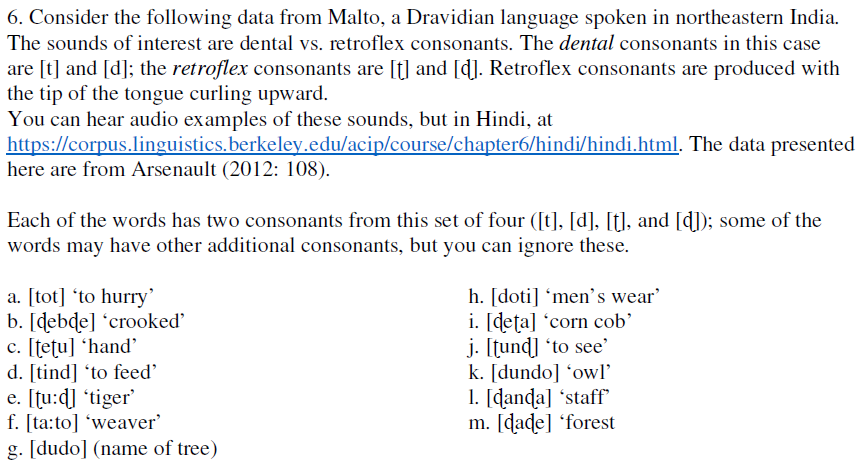
\includegraphics{../images/malto.png}
\end{figure}

~\\
INSTRUCTOR NOTES: It is not possible to have stops of different places of articulation co-occurring in a single word. Instead, if there are two stops, both must be dental, or both must be retroflex. For example, it’s possible to have a word with two dental stops, as in [tot] ‘to hurry’ (even if they disagree in voicing, as in [tind] ‘to feed’), or a word with two retroflex stops, as in [ɖebɖe] ‘crooked’ (again, regardless of voicing, as in [ɖeʈa] ‘corn cob’). But there are no words that have one dental and one retroflex stop, in either order, regardless of voicing. (accurate, generalizations, concrete examples)


\vfill
Excellent (3) ~~~ Good (2.2) ~~~ Fair (1.7) ~~~ Poor (0)
\newpage

{\large Question 5}\\

Topic: Phonological Relationships and Analysis\\
Source: Week 6 Handout, Question 11\\

What do the two signs below tell you about the phonological status of \underline{handshape} in ASL, and why?\\

\begin{figure}[H]
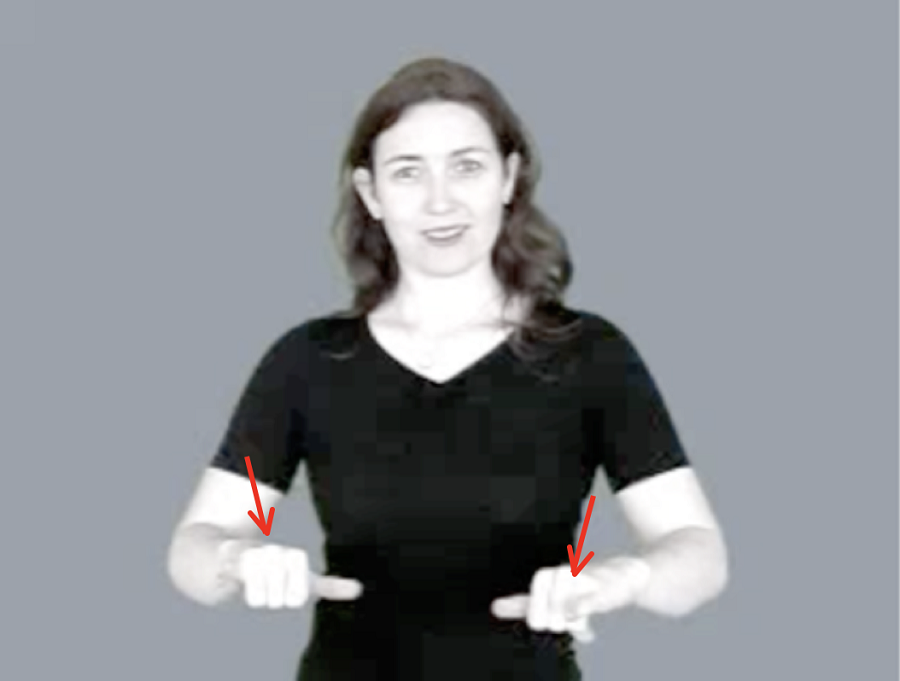
\includegraphics{../images/asl_stay.png}
\caption{STAY}
\end{figure}
\begin{figure}[H]
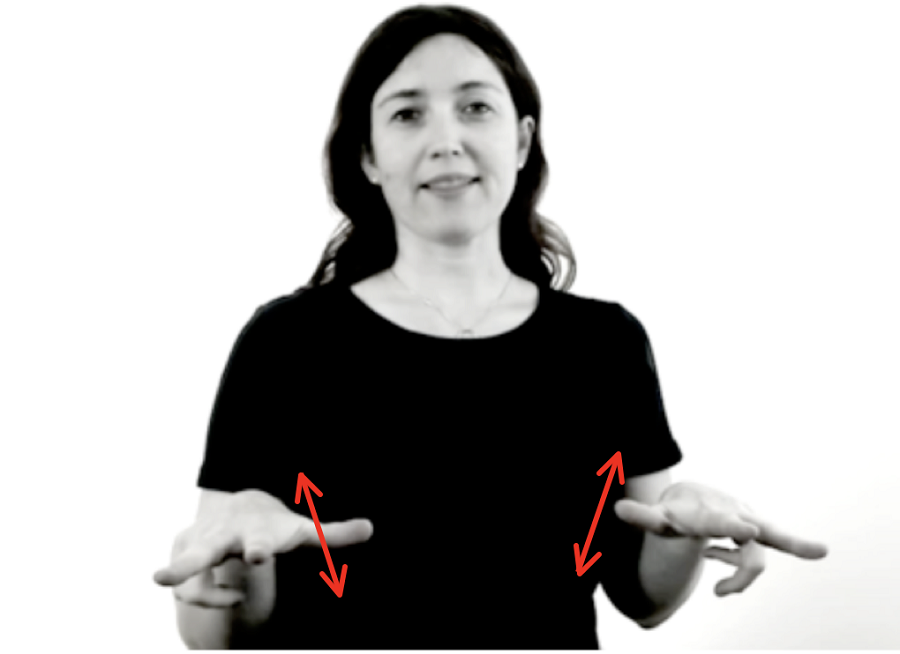
\includegraphics{../images/asl_awkward.png}
\caption{AWKWARD}
\end{figure}

~\\
INSTRUCTOR NOTES: nothing, because both handshape and movement are different


\vfill
Excellent (3) ~~~ Good (2.2) ~~~ Fair (1.7) ~~~ Poor (0)
\newpage

\begin{center}
\textbf{{\color{red}{\HUGE END OF EXAM}}}\\

\end{center}
\newpage

\begin{center}
\textbf{{\color{blue}{\HUGE START OF EXAM\\}}}

\textbf{{\color{blue}{\HUGE Student ID: 11061\\}}}

\textbf{{\color{blue}{\HUGE \\}}}

\end{center}
\newpage

{\large Question 1}\\

Topic: Transcription\\
Source: Quiz 1, Question 10\\

Explain whether this word either does or does not have an [ʃ] sound in it, and why the spelling and pronunciation either do or do not align.\\

<facial>


~\\
INSTRUCTOR NOTES: 


\vfill
Excellent (3) ~~~ Good (2.2) ~~~ Fair (1.7) ~~~ Poor (0)
\newpage

{\large Question 2}\\

Topic: Articulatory Phonetics\\
Source: Week 3 Discussion\\

Assuming a Standard North American English inventory, does this vowel need to have tenseness specified if you're giving a prose description? Why or why not?\\

{[ɑ]}


~\\
INSTRUCTOR NOTES: no


\vfill
Excellent (3) ~~~ Good (2.2) ~~~ Fair (1.7) ~~~ Poor (0)
\newpage

{\large Question 3}\\

Topic: Phonological Features\\
Source: Homework 2, Question 1\\

Explain which sound should be removed to make this a natural class (assuming SNAE, except that there are no diphthongs, no [ə] or [ʌ], no syllabic consonants, and no [w̥]), and what the minimum set of features would be to describe the resulting natural class.\\

{[i]}, {[ɪ]}, {[ɛ]}, {[u]}, {[ʊ]}


~\\
INSTRUCTOR NOTES: [ɛ] should be removed, so that we have the natural class of high vowels; this could be minimally represented with [+syll, +high]


\vfill
Excellent (3) ~~~ Good (2.2) ~~~ Fair (1.7) ~~~ Poor (0)
\newpage

{\large Question 4}\\

Topic: Skewed Distributions\\
Source: Week 5 Handout, Question 7\\

Explain how you would go about looking for co-occurrence restrictions in bi-syllabic signs in ASL. (Refer to the data that follows.)\\

\begin{figure}[H]
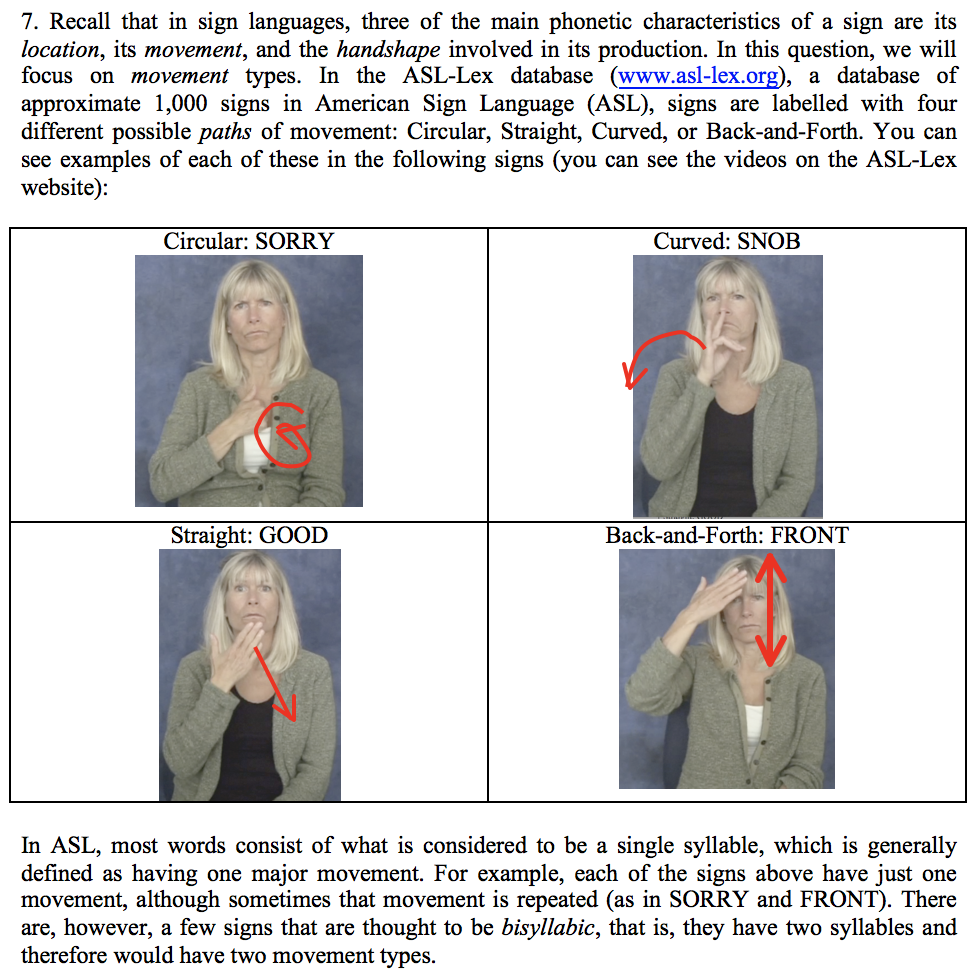
\includegraphics{../images/ASL_movement.png}
\end{figure}

~\\
INSTRUCTOR NOTES: You would start by coming up with all the possible combinations expected (i.e., 4x4 = 16). Then you'd compare that to some database of signs in ASL and see which combinations are actually attested or unattested.


\vfill
Excellent (3) ~~~ Good (2.2) ~~~ Fair (1.7) ~~~ Poor (0)
\newpage

{\large Question 5}\\

Topic: Phonological Relationships and Analysis\\
Source: Week 7 Handout, Question 12\\

What is the basic analysis of oral and nasal vowels in this dataset, and what are the key pieces of evidence?\\

\begin{figure}[H]
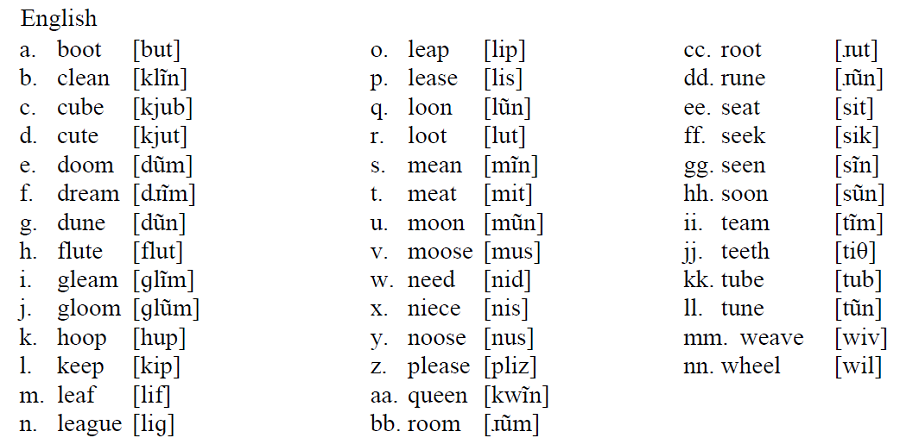
\includegraphics{../images/english12.png}
\end{figure}

~\\
INSTRUCTOR NOTES: The pairs of sounds [i] and [ĩ], and [u] and [ũ], are each allophonic and therefore allophones of the same phoneme in English (though the two pairs represent two contrastive phonemes in English). The sounds [i] and [ĩ] are in complementary distribution in English, with [ĩ] occurring before the sounds [m] and [n], (e.g., [ɡlĩm] ‘gleam’ and [klĩn] ‘clean’) and [i] occurring elsewhere (e.g., [lip] ‘leap’). Similarly, the sounds [u] and [ũ] are also in complementary distribution, with exactly the same conditioning environments: [ũ] occurs before [m] and [n] (e.g., [dũm] ‘doom’ and [dũn] ‘dune’), and [u] occurs elsewhere (e.g. [but] ‘boot’). Thus, within each pair, we treat the vowels as allophonic. 


\vfill
Excellent (3) ~~~ Good (2.2) ~~~ Fair (1.7) ~~~ Poor (0)
\newpage

\begin{center}
\textbf{{\color{red}{\HUGE END OF EXAM}}}\\

\end{center}
\newpage

\begin{center}
\textbf{{\color{blue}{\HUGE START OF EXAM\\}}}

\textbf{{\color{blue}{\HUGE Student ID: 11196\\}}}

\textbf{{\color{blue}{\HUGE \\}}}

\end{center}
\newpage

{\large Question 1}\\

Topic: Transcription\\
Source: Quiz 1, Question 10\\

Explain whether this word either does or does not have an [ʃ] sound in it, and why the spelling and pronunciation either do or do not align.\\

<bassoon>


~\\
INSTRUCTOR NOTES: 


\vfill
Excellent (3) ~~~ Good (2.2) ~~~ Fair (1.7) ~~~ Poor (0)
\newpage

{\large Question 2}\\

Topic: Articulatory Phonetics\\
Source: Quiz 2, Question 6\\

In the pronunciation of this word, which sounds are obstruents and which are sonorants? Explain your answer.\\

<language>


~\\
INSTRUCTOR NOTES: [læŋɡwɪdʒ] -- sonorants: [læŋwɪ] and obstruents: [ɡdʒ]


\vfill
Excellent (3) ~~~ Good (2.2) ~~~ Fair (1.7) ~~~ Poor (0)
\newpage

{\large Question 3}\\

Topic: Phonological Features\\
Source: Week 4 Discussion\\

Explain why the given feature's value varies across this set of sounds.\\

{[anterior]}

fricatives


~\\
INSTRUCTOR NOTES: can have both [+] and [-] anterior fricatives (e.g., [s] and [θ] are [+ant], [ʃ] is [-ant] -- extra good if they also notice you can have [0 ant] like [f], which isn't [CORONAL]


\vfill
Excellent (3) ~~~ Good (2.2) ~~~ Fair (1.7) ~~~ Poor (0)
\newpage

{\large Question 4}\\

Topic: Skewed Distributions\\
Source: Week 5 Handout, Question 7\\

Explain how you would go about looking for co-occurrence restrictions in bi-syllabic signs in ASL. (Refer to the data that follows.)\\

\begin{figure}[H]
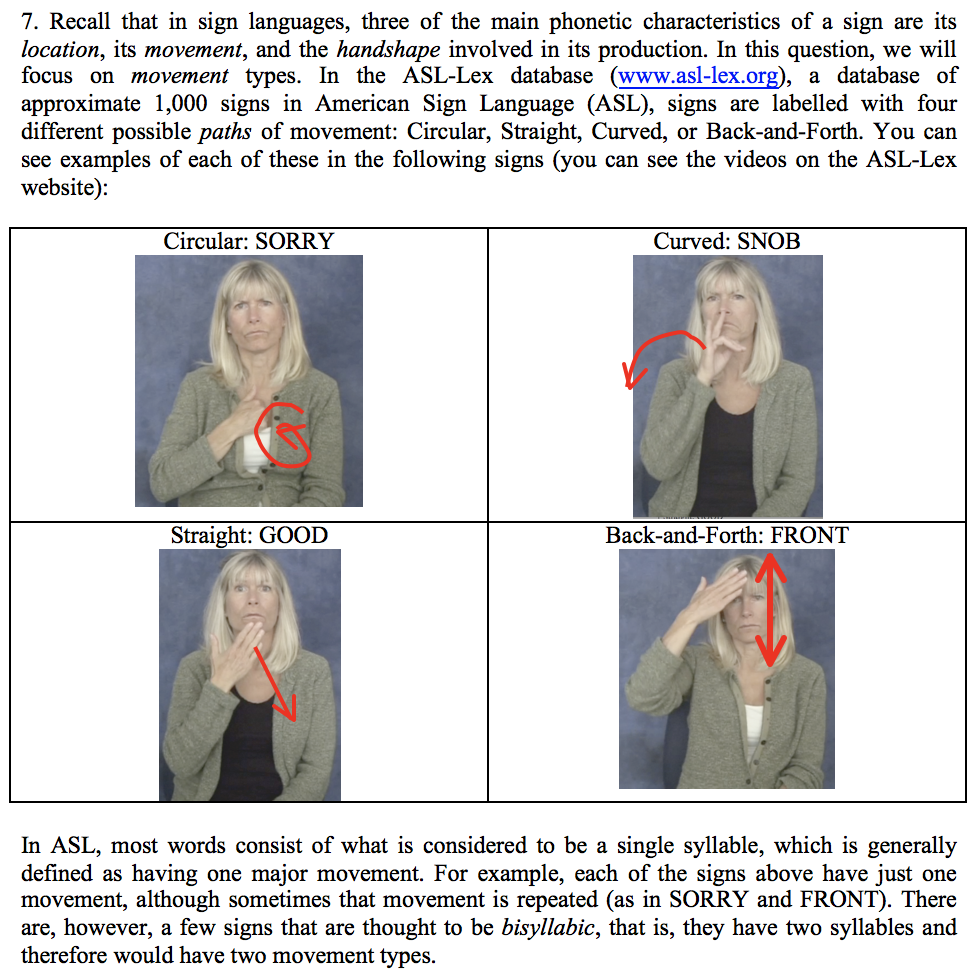
\includegraphics{../images/ASL_movement.png}
\end{figure}

~\\
INSTRUCTOR NOTES: You would start by coming up with all the possible combinations expected (i.e., 4x4 = 16). Then you'd compare that to some database of signs in ASL and see which combinations are actually attested or unattested.


\vfill
Excellent (3) ~~~ Good (2.2) ~~~ Fair (1.7) ~~~ Poor (0)
\newpage

{\large Question 5}\\

Topic: Phonological Relationships and Analysis\\
Source: Week 7 Handout, Question 9\\

What is the basic analysis of vowel length in this dataset, and what are the key pieces of evidence?\\

\begin{figure}[H]
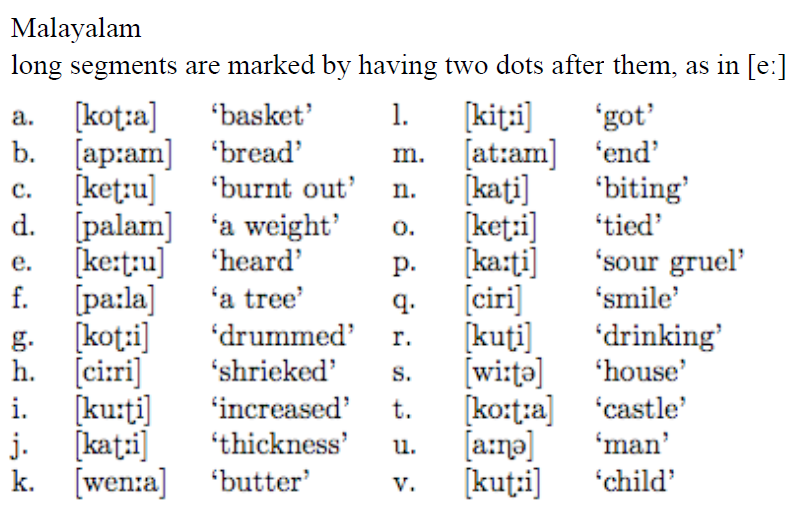
\includegraphics{../images/malayalam.png}
\end{figure}

~\\
INSTRUCTOR NOTES: Short and long vowels appear to be contrastive (phonemic) in Malayalam, as evidenced by minimal pairs that differ only in terms of their vowel length, such as [koʈːa] ‘basket’ vs. [koːʈːa] ‘castle’ or [keʈːu] ‘burnt out’ vs. [keːʈːu] ‘heard.’


\vfill
Excellent (3) ~~~ Good (2.2) ~~~ Fair (1.7) ~~~ Poor (0)
\newpage

\begin{center}
\textbf{{\color{red}{\HUGE END OF EXAM}}}\\

\end{center}
\newpage

\begin{center}
\textbf{{\color{blue}{\HUGE START OF EXAM\\}}}

\textbf{{\color{blue}{\HUGE Student ID: 11661\\}}}

\textbf{{\color{blue}{\HUGE \\}}}

\end{center}
\newpage

{\large Question 1}\\

Topic: Transcription\\
Source: Week 2 Handout, Part II, Question 3\\

Explain why people might legitimately disagree about how many sounds this particular word contains.\\

<worse>


~\\
INSTRUCTOR NOTES: 


\vfill
Excellent (3) ~~~ Good (2.2) ~~~ Fair (1.7) ~~~ Poor (0)
\newpage

{\large Question 2}\\

Topic: Articulatory Phonetics\\
Source: Week 3 Handout, Question 3\\

Explain why the additional vowel below either does or does not belong in the phonetic natural class defined by the original set of SNAE vowels.\\

Original set: {[ɛ]}, {[ɪ]}, {[ʊ]}, {[ɔ]}

Addition: {[ɑ]}


~\\
INSTRUCTOR NOTES: new vowel is a low vowel; should recognize that there's more than one decision about low vowels and tenseness; default is to say it doesn't belong in the class because tenseness is irrelevant


\vfill
Excellent (3) ~~~ Good (2.2) ~~~ Fair (1.7) ~~~ Poor (0)
\newpage

{\large Question 3}\\

Topic: Phonological Features\\
Source: Week 4 Discussion\\

Explain why the given feature's value varies across this set of sounds.\\

{[anterior]}

fricatives


~\\
INSTRUCTOR NOTES: can have both [+] and [-] anterior fricatives (e.g., [s] and [θ] are [+ant], [ʃ] is [-ant] -- extra good if they also notice you can have [0 ant] like [f], which isn't [CORONAL]


\vfill
Excellent (3) ~~~ Good (2.2) ~~~ Fair (1.7) ~~~ Poor (0)
\newpage

{\large Question 4}\\

Topic: Skewed Distributions\\
Source: Quiz 4, Question 3\\

L$_X$ (Language X) has three vowels, [i], [a], and [u]. L$_X$ has tetra-syllabic roots. If L$_X$ does not allow non-identical high vowels to co-occur, which one of the following tetra-syllabic vocalic sequences do you predict to be unattested in L$_X$? Explain why.\\

\begin{itemize} \item {[i...i...u...u]} \item {[a...a...i...i]} \item {[u...u...u...u]} \item {[i...i...i...a]} \end{itemize}


~\\
INSTRUCTOR NOTES: [i...i...u...u]


\vfill
Excellent (3) ~~~ Good (2.2) ~~~ Fair (1.7) ~~~ Poor (0)
\newpage

{\large Question 5}\\

Topic: Phonological Relationships and Analysis\\
Source: Week 6 Handout, Question 11\\

What do the two signs below tell you about the phonological status of \underline{handshape} in ASL, and why?\\

\begin{figure}[H]
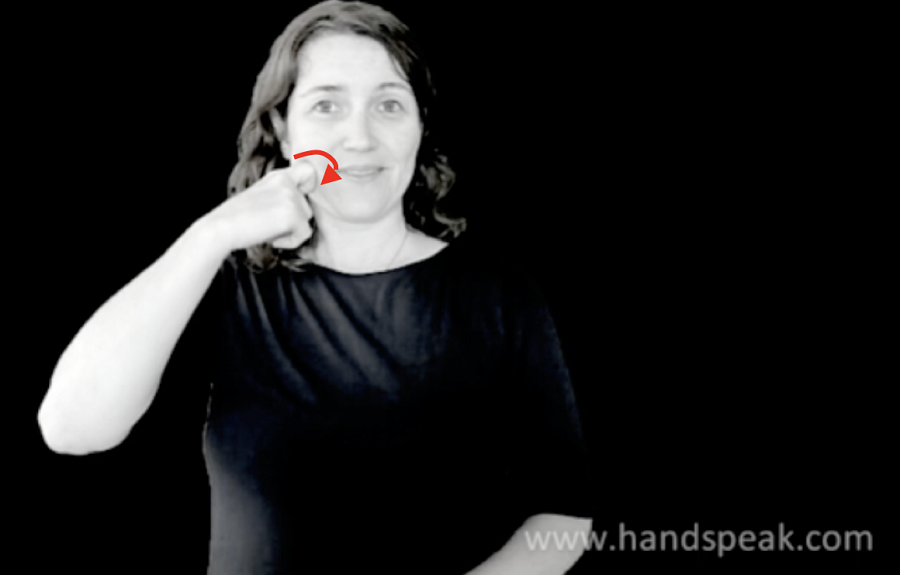
\includegraphics{../images/asl_apple.png}
\caption{APPLE}
\end{figure}
\begin{figure}[H]
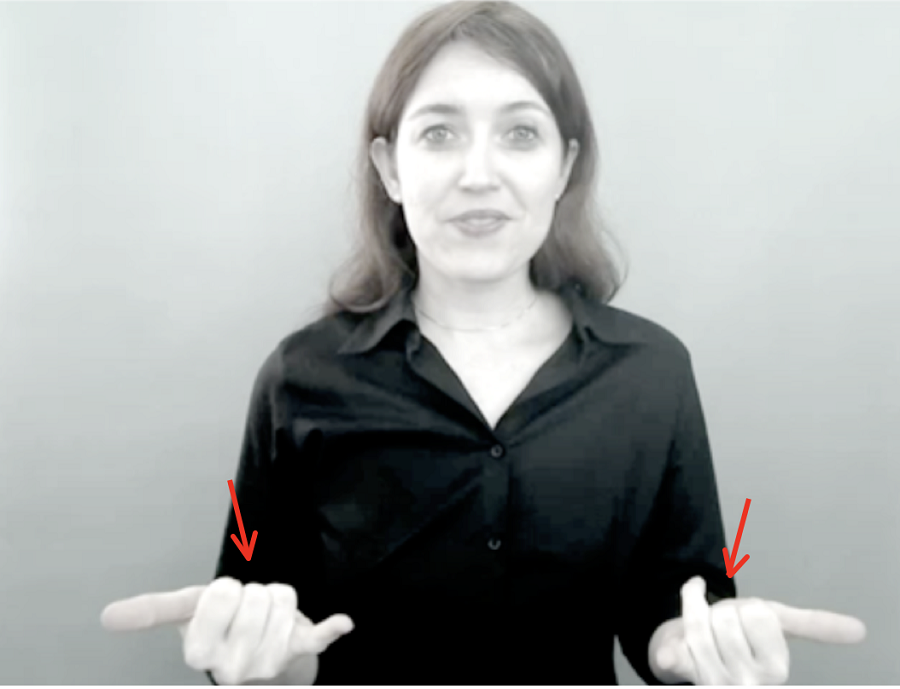
\includegraphics{../images/asl_now.png}
\caption{NOW}
\end{figure}

~\\
INSTRUCTOR NOTES: nothing, because handshape and location and movement are all also different


\vfill
Excellent (3) ~~~ Good (2.2) ~~~ Fair (1.7) ~~~ Poor (0)
\newpage

\begin{center}
\textbf{{\color{red}{\HUGE END OF EXAM}}}\\

\end{center}
\newpage

\begin{center}
\textbf{{\color{blue}{\HUGE START OF EXAM\\}}}

\textbf{{\color{blue}{\HUGE Student ID: 11925\\}}}

\textbf{{\color{blue}{\HUGE \\}}}

\end{center}
\newpage

{\large Question 1}\\

Topic: Transcription\\
Source: Week 2 Handout, Part II\\

Is this a reasonable transcription of this word? Explain why.\\

<mouse>: {[mɔɪs]}


~\\
INSTRUCTOR NOTES: no, [ɑʊ]


\vfill
Excellent (3) ~~~ Good (2.2) ~~~ Fair (1.7) ~~~ Poor (0)
\newpage

{\large Question 2}\\

Topic: Articulatory Phonetics\\
Source: Week 3 Handout, Question 13\\

Explain why this image does or does not match the description.\\

\begin{itemize} \item A two-handed sign. \item Location: In front of signer’s chin. \item Handshape: Starts with an “L” shape; index finger and thumb come together during the sign. \item Movement: Hands start crossed and then move away from each other horizontally. \end{itemize}

\begin{figure}[H]
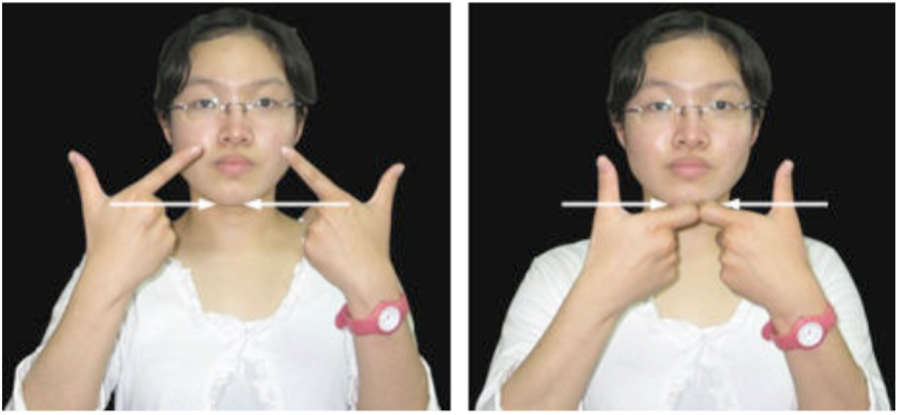
\includegraphics{../images/taiwansign_fit.png}
\caption{FIT}
\end{figure}

~\\
INSTRUCTOR NOTES: no; hands don't start crossed, and handshape change is wrong


\vfill
Excellent (3) ~~~ Good (2.2) ~~~ Fair (1.7) ~~~ Poor (0)
\newpage

{\large Question 3}\\

Topic: Phonological Features\\
Source: Homework 2, Question 1\\

Explain which sound should be removed to make this a natural class (assuming SNAE, except that there are no diphthongs, no [ə] or [ʌ], no syllabic consonants, and no [w̥]), and what the minimum set of features would be to describe the resulting natural class.\\

{[i]}, {[ɪ]}, {[ɛ]}, {[u]}, {[ʊ]}


~\\
INSTRUCTOR NOTES: [ɛ] should be removed, so that we have the natural class of high vowels; this could be minimally represented with [+syll, +high]


\vfill
Excellent (3) ~~~ Good (2.2) ~~~ Fair (1.7) ~~~ Poor (0)
\newpage

{\large Question 4}\\

Topic: Skewed Distributions\\
Source: Week 5 Handout, Question 6\\

Explain why the following table would not be a good way of organizing the data for Malto.\\

\begin{figure}[H]
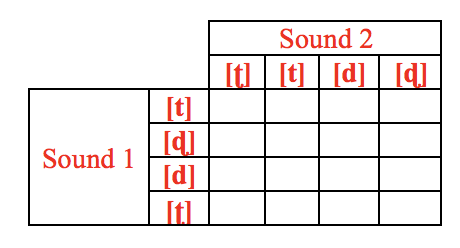
\includegraphics{../images/Malto_table_bad.png}
\end{figure}

~\\
INSTRUCTOR NOTES: rows and columns not in same order; rows not organized by phonetic characteristic; specifically, instructions ask about dental vs. retroflex, so should be organized around those


\vfill
Excellent (3) ~~~ Good (2.2) ~~~ Fair (1.7) ~~~ Poor (0)
\newpage

{\large Question 5}\\

Topic: Phonological Relationships and Analysis\\
Source: Week 7 Handout, Question 9\\

What is the basic analysis of vowel length in this dataset, and what are the key pieces of evidence?\\

\begin{figure}[H]
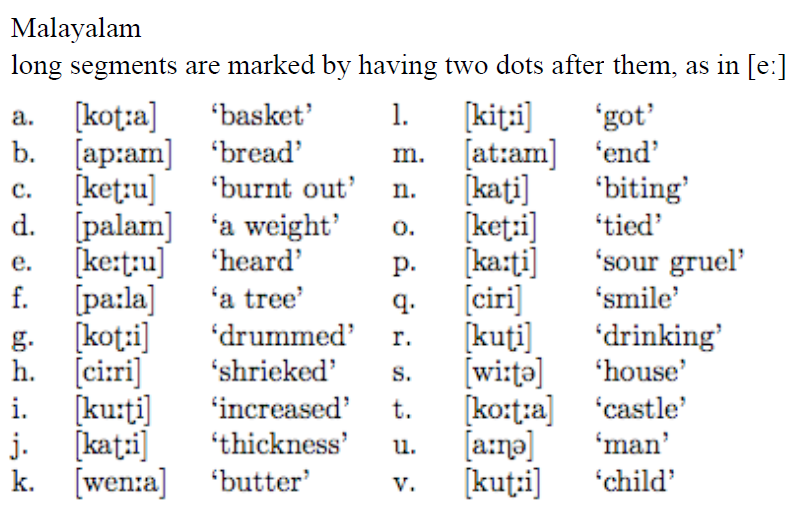
\includegraphics{../images/malayalam.png}
\end{figure}

~\\
INSTRUCTOR NOTES: Short and long vowels appear to be contrastive (phonemic) in Malayalam, as evidenced by minimal pairs that differ only in terms of their vowel length, such as [koʈːa] ‘basket’ vs. [koːʈːa] ‘castle’ or [keʈːu] ‘burnt out’ vs. [keːʈːu] ‘heard.’


\vfill
Excellent (3) ~~~ Good (2.2) ~~~ Fair (1.7) ~~~ Poor (0)
\newpage

\begin{center}
\textbf{{\color{red}{\HUGE END OF EXAM}}}\\

\end{center}
\newpage

\begin{center}
\textbf{{\color{blue}{\HUGE START OF EXAM\\}}}

\textbf{{\color{blue}{\HUGE Student ID: 12377\\}}}

\textbf{{\color{blue}{\HUGE \\}}}

\end{center}
\newpage

{\large Question 1}\\

Topic: Transcription\\
Source: Week 2 Handout, Part II, Question 11\\

How would this word be transcribed?\\ (Kathleen will then ask a follow-up question about your transcription.)\\

<cough>


~\\
INSTRUCTOR NOTES: [kɑf]


\vfill
Excellent (3) ~~~ Good (2.2) ~~~ Fair (1.7) ~~~ Poor (0)
\newpage

{\large Question 2}\\

Topic: Articulatory Phonetics\\
Source: Week 3 Handout, Question 7\\

Is the symbol given a reasonable way to transcribe any of the sounds described below? If so, which one? If not, why not? Explain your answer.\\

{[n]}

\begin{itemize} \item voiceless palatal affricate \item voiced velar nasal \item voiceless glottal fricative \item voiced labiodental fricative \item voiced interdental fricative \item voiced palatal fricative \end{itemize}


~\\
INSTRUCTOR NOTES: no (voiced alveolar nasal)


\vfill
Excellent (3) ~~~ Good (2.2) ~~~ Fair (1.7) ~~~ Poor (0)
\newpage

{\large Question 3}\\

Topic: Phonological Features\\
Source: Quiz 3, Question 12\\

Explain how you figure out which feature is involved in the process of umlaut shown below.\\

\begin{figure}[H]
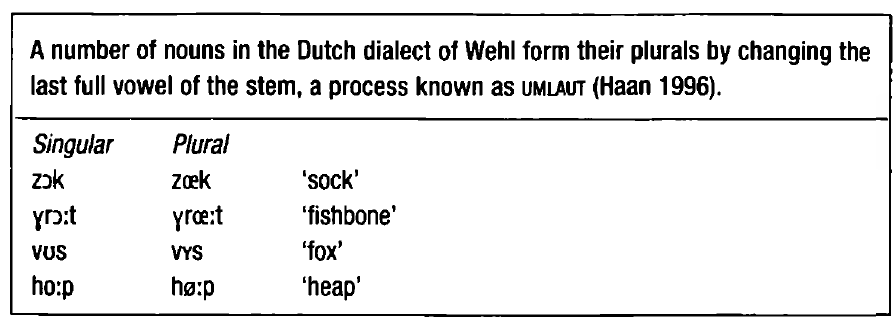
\includegraphics{../images/dutch.png}
\end{figure}

~\\
INSTRUCTOR NOTES: we look to see which vowels are affected, and compare them to see which feature is DIFFERENT (not e.g. what features they share); so since the vowels in the singular and plural are identical except that the singular forms are back and the plural are front, it's the feature [back] that is relevant / changing / involved (not e.g. the feature [round] just because all of the vowels are round)


\vfill
Excellent (3) ~~~ Good (2.2) ~~~ Fair (1.7) ~~~ Poor (0)
\newpage

{\large Question 4}\\

Topic: Skewed Distributions\\
Source: Week 5 Handout, Question 1\\

Explain why we think that languages are not random in terms of their phonology.\\


~\\
INSTRUCTOR NOTES: 


\vfill
Excellent (3) ~~~ Good (2.2) ~~~ Fair (1.7) ~~~ Poor (0)
\newpage

{\large Question 5}\\

Topic: Phonological Relationships and Analysis\\
Source: Week 6 Handout, Question 11\\

What do the two signs below tell you about the phonological status of \underline{handshape} in ASL, and why?\\

\begin{figure}[H]
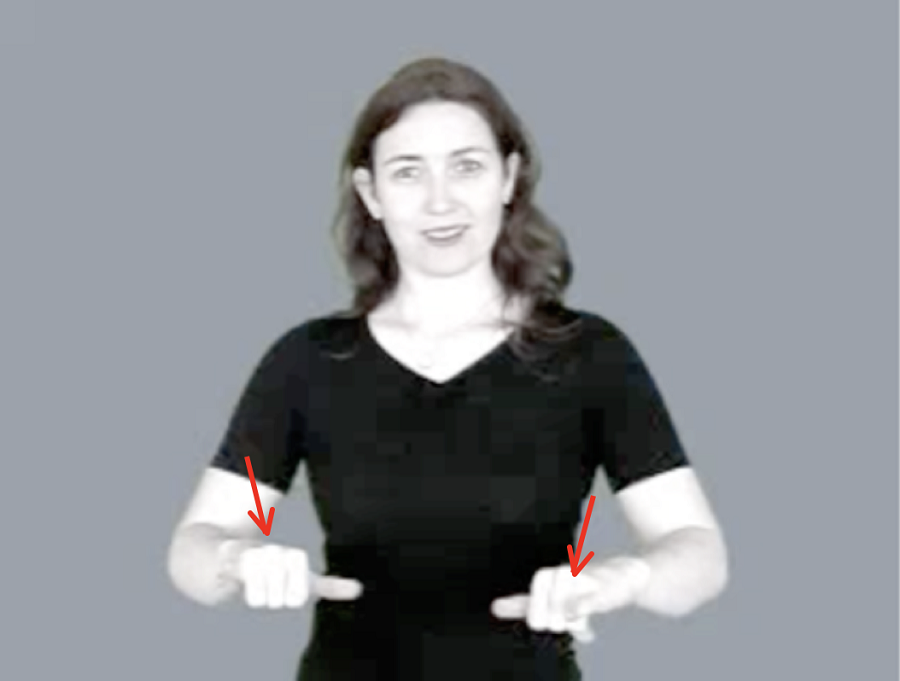
\includegraphics{../images/asl_stay.png}
\caption{STAY}
\end{figure}
\begin{figure}[H]
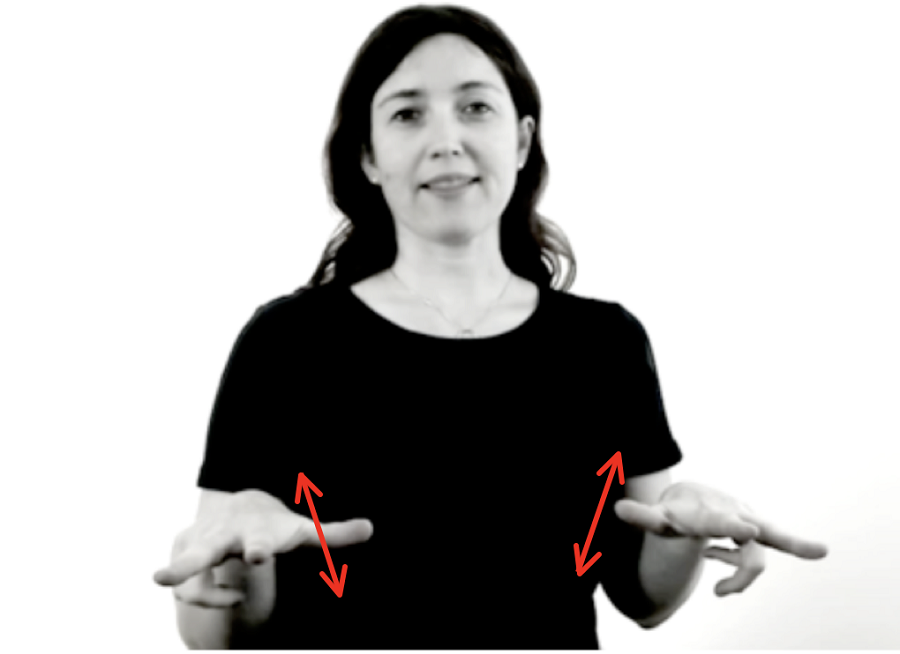
\includegraphics{../images/asl_awkward.png}
\caption{AWKWARD}
\end{figure}

~\\
INSTRUCTOR NOTES: nothing, because both handshape and movement are different


\vfill
Excellent (3) ~~~ Good (2.2) ~~~ Fair (1.7) ~~~ Poor (0)
\newpage

\begin{center}
\textbf{{\color{red}{\HUGE END OF EXAM}}}\\

\end{center}
\newpage

\begin{center}
\textbf{{\color{blue}{\HUGE START OF EXAM\\}}}

\textbf{{\color{blue}{\HUGE Student ID: 12991\\}}}

\textbf{{\color{blue}{\HUGE \\}}}

\end{center}
\newpage

{\large Question 1}\\

Topic: Transcription\\
Source: Week 2 Handout, Part II, Question 11\\

How would this word be transcribed?\\ (Kathleen will then ask a follow-up question about your transcription.)\\

<goat>


~\\
INSTRUCTOR NOTES: [ɡoʊt]


\vfill
Excellent (3) ~~~ Good (2.2) ~~~ Fair (1.7) ~~~ Poor (0)
\newpage

{\large Question 2}\\

Topic: Articulatory Phonetics\\
Source: Homework 1, Question 3(b)\\

Explain why this is or is not a complete phonetic natural class in standard North American English.\\

{[ɔ]}, {[ʊ]}, {[u]}, {[oʊ]}


~\\
INSTRUCTOR NOTES: yes (all back rounded vowels)


\vfill
Excellent (3) ~~~ Good (2.2) ~~~ Fair (1.7) ~~~ Poor (0)
\newpage

{\large Question 3}\\

Topic: Phonological Features\\
Source: Quiz 3, Question 6\\

Explain why this is an incorrect statement.\\

Nasal consonants are {[-continuant]}, because they cannot be produced for an extended period of time.


~\\
INSTRUCTOR NOTES: nasals are indeed [-cont], but they can be held for a long time -- it's just that air isn't coming from the mouth


\vfill
Excellent (3) ~~~ Good (2.2) ~~~ Fair (1.7) ~~~ Poor (0)
\newpage

{\large Question 4}\\

Topic: Skewed Distributions\\
Source: Week 5 Handout, Question 6\\

If I gave you a new word in Malto, [di\_\_u], would it be possible to predict whether it's [d] or [t] that goes in the blank? Explain why or why not.\\

\begin{figure}[H]
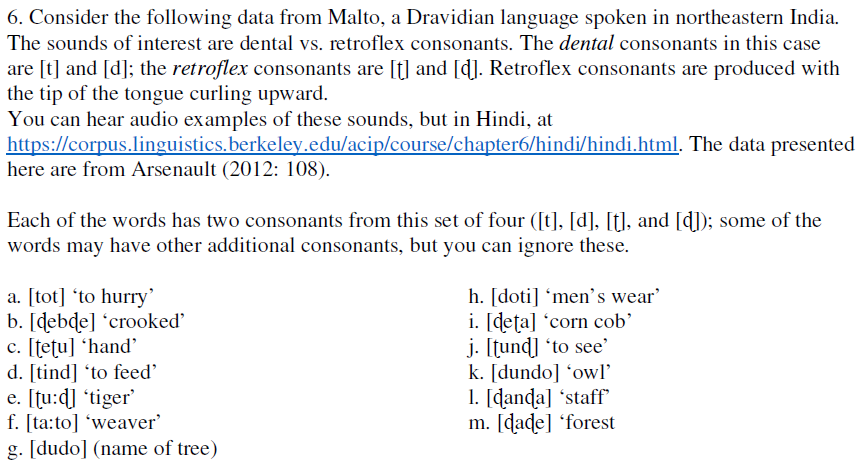
\includegraphics{../images/malto.png}
\end{figure}

~\\
INSTRUCTOR NOTES: No, it's not possible. In Malto, you can predict that there are two dental or two retroflex stops in a word, but you can't predict the voicing. These two sounds are both dental, so there's no way to predict.


\vfill
Excellent (3) ~~~ Good (2.2) ~~~ Fair (1.7) ~~~ Poor (0)
\newpage

{\large Question 5}\\

Topic: Phonological Relationships and Analysis\\
Source: Week 7 Handout, Question 12\\

What is the basic analysis of oral and nasal vowels in this dataset, and what are the key pieces of evidence?\\

\begin{figure}[H]
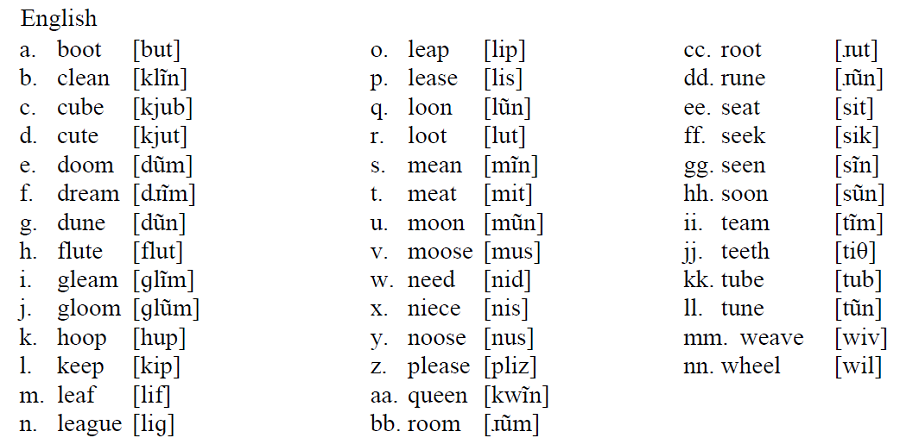
\includegraphics{../images/english12.png}
\end{figure}

~\\
INSTRUCTOR NOTES: The pairs of sounds [i] and [ĩ], and [u] and [ũ], are each allophonic and therefore allophones of the same phoneme in English (though the two pairs represent two contrastive phonemes in English). The sounds [i] and [ĩ] are in complementary distribution in English, with [ĩ] occurring before the sounds [m] and [n], (e.g., [ɡlĩm] ‘gleam’ and [klĩn] ‘clean’) and [i] occurring elsewhere (e.g., [lip] ‘leap’). Similarly, the sounds [u] and [ũ] are also in complementary distribution, with exactly the same conditioning environments: [ũ] occurs before [m] and [n] (e.g., [dũm] ‘doom’ and [dũn] ‘dune’), and [u] occurs elsewhere (e.g. [but] ‘boot’). Thus, within each pair, we treat the vowels as allophonic. 


\vfill
Excellent (3) ~~~ Good (2.2) ~~~ Fair (1.7) ~~~ Poor (0)
\newpage

\begin{center}
\textbf{{\color{red}{\HUGE END OF EXAM}}}\\

\end{center}
\newpage

\begin{center}
\textbf{{\color{blue}{\HUGE START OF EXAM\\}}}

\textbf{{\color{blue}{\HUGE Student ID: 13570\\}}}

\textbf{{\color{blue}{\HUGE \\}}}

\end{center}
\newpage

{\large Question 1}\\

Topic: Transcription\\
Source: Quiz 1, Question 10\\

Explain whether this word either does or does not have an [ʃ] sound in it, and why the spelling and pronunciation either do or do not align.\\

<meticulous>


~\\
INSTRUCTOR NOTES: 


\vfill
Excellent (3) ~~~ Good (2.2) ~~~ Fair (1.7) ~~~ Poor (0)
\newpage

{\large Question 2}\\

Topic: Articulatory Phonetics\\
Source: Homework 1, Question 3(b)\\

Explain why this is or is not a complete phonetic natural class in standard North American English.\\

{[ɔ]}, {[ʊ]}, {[u]}, {[oʊ]}


~\\
INSTRUCTOR NOTES: yes (all back rounded vowels)


\vfill
Excellent (3) ~~~ Good (2.2) ~~~ Fair (1.7) ~~~ Poor (0)
\newpage

{\large Question 3}\\

Topic: Phonological Features\\
Source: Week 4 Discussion\\

Explain what the given feature’s value is for this class of sounds, and why.\\

{[approximant]}

nasals


~\\
INSTRUCTOR NOTES: [-], because air can't escape through the mouth ([+approx] sounds have a narrowing in the vocal tract, but air escapes without friction)


\vfill
Excellent (3) ~~~ Good (2.2) ~~~ Fair (1.7) ~~~ Poor (0)
\newpage

{\large Question 4}\\

Topic: Skewed Distributions\\
Source: Week 5 Handout, Question 7\\

Explain how you would go about looking for co-occurrence restrictions in bi-syllabic signs in ASL. (Refer to the data that follows.)\\

\begin{figure}[H]
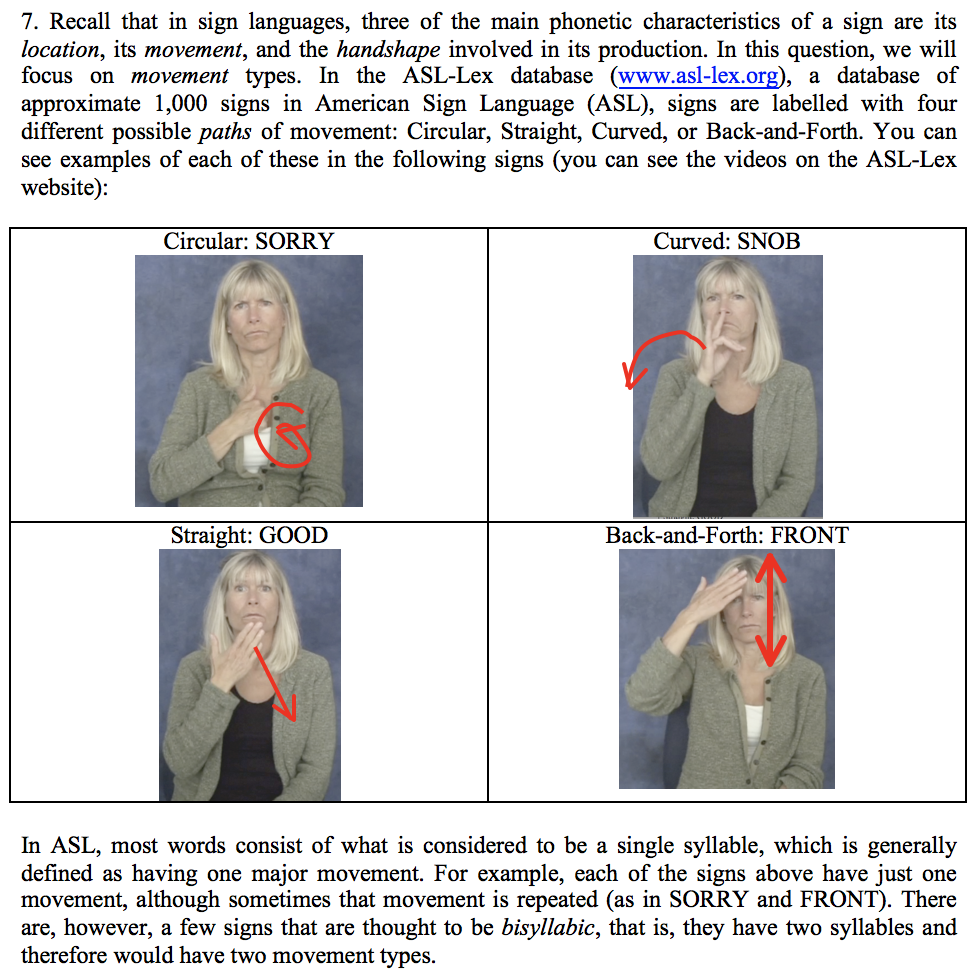
\includegraphics{../images/ASL_movement.png}
\end{figure}

~\\
INSTRUCTOR NOTES: You would start by coming up with all the possible combinations expected (i.e., 4x4 = 16). Then you'd compare that to some database of signs in ASL and see which combinations are actually attested or unattested.


\vfill
Excellent (3) ~~~ Good (2.2) ~~~ Fair (1.7) ~~~ Poor (0)
\newpage

{\large Question 5}\\

Topic: Phonological Relationships and Analysis\\
Source: Week 7 Handout, Question 12\\

What is the basic analysis of oral and nasal vowels in this dataset, and what are the key pieces of evidence?\\

\begin{figure}[H]
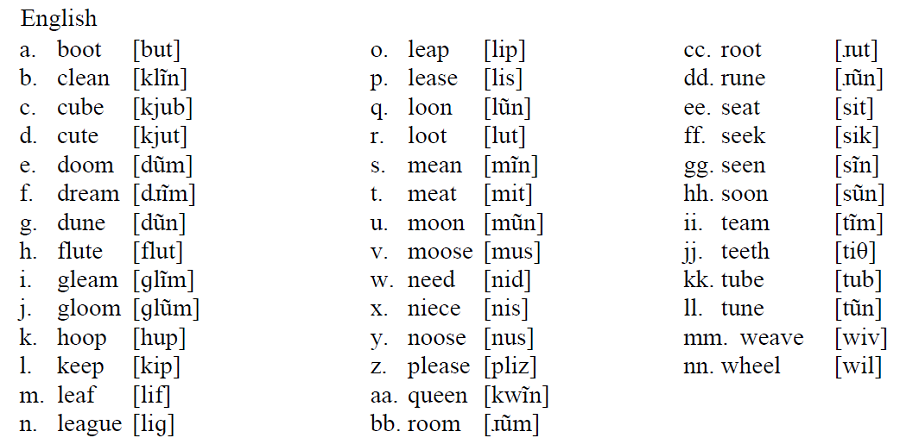
\includegraphics{../images/english12.png}
\end{figure}

~\\
INSTRUCTOR NOTES: The pairs of sounds [i] and [ĩ], and [u] and [ũ], are each allophonic and therefore allophones of the same phoneme in English (though the two pairs represent two contrastive phonemes in English). The sounds [i] and [ĩ] are in complementary distribution in English, with [ĩ] occurring before the sounds [m] and [n], (e.g., [ɡlĩm] ‘gleam’ and [klĩn] ‘clean’) and [i] occurring elsewhere (e.g., [lip] ‘leap’). Similarly, the sounds [u] and [ũ] are also in complementary distribution, with exactly the same conditioning environments: [ũ] occurs before [m] and [n] (e.g., [dũm] ‘doom’ and [dũn] ‘dune’), and [u] occurs elsewhere (e.g. [but] ‘boot’). Thus, within each pair, we treat the vowels as allophonic. 


\vfill
Excellent (3) ~~~ Good (2.2) ~~~ Fair (1.7) ~~~ Poor (0)
\newpage

\begin{center}
\textbf{{\color{red}{\HUGE END OF EXAM}}}\\

\end{center}
\newpage

\begin{center}
\textbf{{\color{blue}{\HUGE START OF EXAM\\}}}

\textbf{{\color{blue}{\HUGE Student ID: 15082\\}}}

\textbf{{\color{blue}{\HUGE \\}}}

\end{center}
\newpage

{\large Question 1}\\

Topic: Transcription\\
Source: Week 2 Handout, Part II, Question 2\\

Explain why people might legitimately disagree about how many sounds this particular word contains.\\

<goat>


~\\
INSTRUCTOR NOTES: 


\vfill
Excellent (3) ~~~ Good (2.2) ~~~ Fair (1.7) ~~~ Poor (0)
\newpage

{\large Question 2}\\

Topic: Articulatory Phonetics\\
Source: Week 3 Handout, Question 9\\

Explain how to figure out what the sound being produced is in this diagram.\\

\begin{figure}[H]
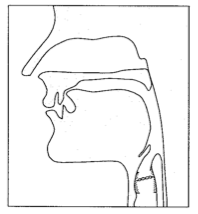
\includegraphics{../images/sagittal_z.png}
\end{figure}

~\\
INSTRUCTOR NOTES: [z] (check voicing, place, manner, and velum)


\vfill
Excellent (3) ~~~ Good (2.2) ~~~ Fair (1.7) ~~~ Poor (0)
\newpage

{\large Question 3}\\

Topic: Phonological Features\\
Source: Quiz 3, Question 12\\

Explain how you figure out which feature is involved in the process of umlaut shown below.\\

\begin{figure}[H]
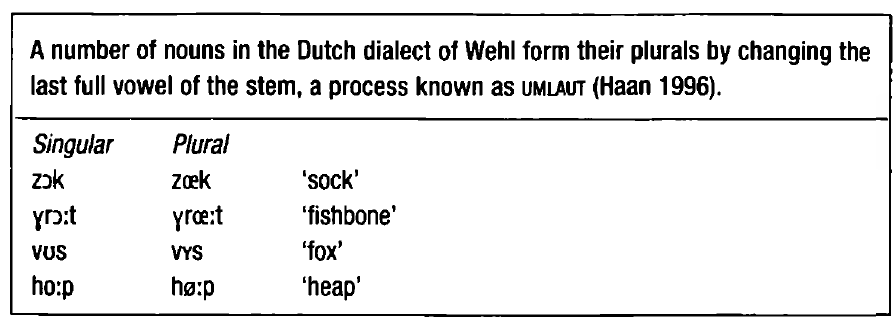
\includegraphics{../images/dutch.png}
\end{figure}

~\\
INSTRUCTOR NOTES: we look to see which vowels are affected, and compare them to see which feature is DIFFERENT (not e.g. what features they share); so since the vowels in the singular and plural are identical except that the singular forms are back and the plural are front, it's the feature [back] that is relevant / changing / involved (not e.g. the feature [round] just because all of the vowels are round)


\vfill
Excellent (3) ~~~ Good (2.2) ~~~ Fair (1.7) ~~~ Poor (0)
\newpage

{\large Question 4}\\

Topic: Skewed Distributions\\
Source: Quiz 4, Question 1\\

L$_X$ (Language X) has three vowels, [i], [a], and [u]. It has bi-syllabic roots like Kikuyu. It does not allow non-identical high vowels to co-occur. Of the following nine logically possible vocalic sequences, which ones should be unattested in L$_X$? Explain why.\\

\begin{itemize} \item {[i...i]} \item {[i...a]} \item {[i...u]} \item {[a...i]} \item {[a...a]} \item {[a...u]} \item {[u...i]} \item {[u...a]} \item {[u...u]} \end{itemize}


~\\
INSTRUCTOR NOTES: [i...u], [u...i]


\vfill
Excellent (3) ~~~ Good (2.2) ~~~ Fair (1.7) ~~~ Poor (0)
\newpage

{\large Question 5}\\

Topic: Phonological Relationships and Analysis\\
Source: Week 7 Handout, Question 12\\

What is the basic analysis of oral and nasal vowels in this dataset, and what are the key pieces of evidence?\\

\begin{figure}[H]
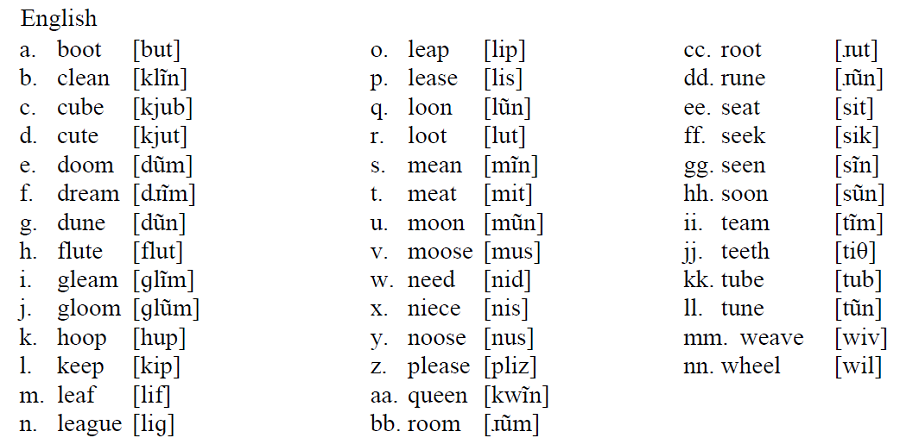
\includegraphics{../images/english12.png}
\end{figure}

~\\
INSTRUCTOR NOTES: The pairs of sounds [i] and [ĩ], and [u] and [ũ], are each allophonic and therefore allophones of the same phoneme in English (though the two pairs represent two contrastive phonemes in English). The sounds [i] and [ĩ] are in complementary distribution in English, with [ĩ] occurring before the sounds [m] and [n], (e.g., [ɡlĩm] ‘gleam’ and [klĩn] ‘clean’) and [i] occurring elsewhere (e.g., [lip] ‘leap’). Similarly, the sounds [u] and [ũ] are also in complementary distribution, with exactly the same conditioning environments: [ũ] occurs before [m] and [n] (e.g., [dũm] ‘doom’ and [dũn] ‘dune’), and [u] occurs elsewhere (e.g. [but] ‘boot’). Thus, within each pair, we treat the vowels as allophonic. 


\vfill
Excellent (3) ~~~ Good (2.2) ~~~ Fair (1.7) ~~~ Poor (0)
\newpage

\begin{center}
\textbf{{\color{red}{\HUGE END OF EXAM}}}\\

\end{center}
\newpage

\begin{center}
\textbf{{\color{blue}{\HUGE START OF EXAM\\}}}

\textbf{{\color{blue}{\HUGE Student ID: 16464\\}}}

\textbf{{\color{blue}{\HUGE \\}}}

\end{center}
\newpage

{\large Question 1}\\

Topic: Transcription\\
Source: Week 2 Handout, Part II, Question 11\\

How would this word be transcribed?\\ (Kathleen will then ask a follow-up question about your transcription.)\\

<goat>


~\\
INSTRUCTOR NOTES: [ɡoʊt]


\vfill
Excellent (3) ~~~ Good (2.2) ~~~ Fair (1.7) ~~~ Poor (0)
\newpage

{\large Question 2}\\

Topic: Articulatory Phonetics\\
Source: Week 3 Handout, Question 7\\

Is the symbol given a reasonable way to transcribe any of the sounds described below? If so, which one? If not, why not? Explain your answer.\\

{[v]}

\begin{itemize} \item voiceless palatal affricate \item voiced velar nasal \item voiceless glottal fricative \item voiced labiodental fricative \item voiced interdental fricative \item voiced palatal fricative \end{itemize}


~\\
INSTRUCTOR NOTES: yes (voiced labiodental fricative)


\vfill
Excellent (3) ~~~ Good (2.2) ~~~ Fair (1.7) ~~~ Poor (0)
\newpage

{\large Question 3}\\

Topic: Phonological Features\\
Source: Week 4 Discussion\\

Explain what the given feature’s value is for this class of sounds, and why.\\

{[approximant]}

nasals


~\\
INSTRUCTOR NOTES: [-], because air can't escape through the mouth ([+approx] sounds have a narrowing in the vocal tract, but air escapes without friction)


\vfill
Excellent (3) ~~~ Good (2.2) ~~~ Fair (1.7) ~~~ Poor (0)
\newpage

{\large Question 4}\\

Topic: Skewed Distributions\\
Source: Week 5 Handout, Question 7\\

Explain how you would go about looking for co-occurrence restrictions in bi-syllabic signs in ASL. (Refer to the data that follows.)\\

\begin{figure}[H]
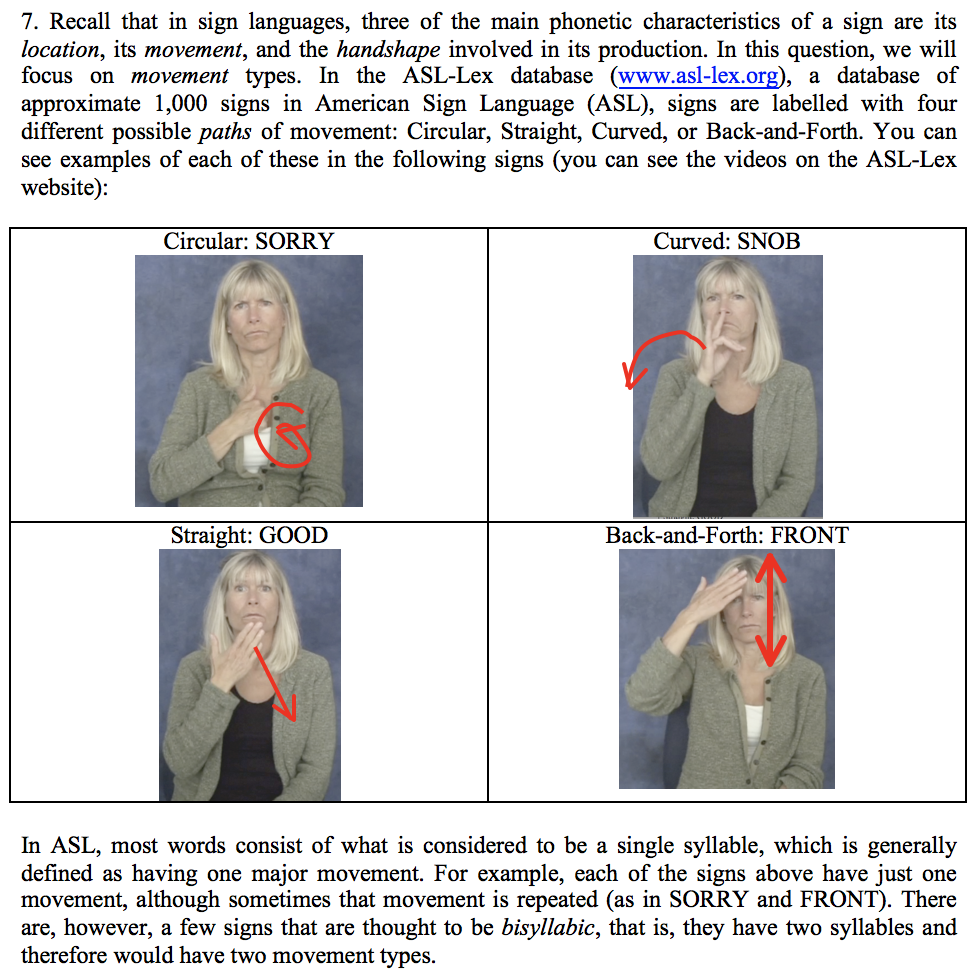
\includegraphics{../images/ASL_movement.png}
\end{figure}

~\\
INSTRUCTOR NOTES: You would start by coming up with all the possible combinations expected (i.e., 4x4 = 16). Then you'd compare that to some database of signs in ASL and see which combinations are actually attested or unattested.


\vfill
Excellent (3) ~~~ Good (2.2) ~~~ Fair (1.7) ~~~ Poor (0)
\newpage

{\large Question 5}\\

Topic: Phonological Relationships and Analysis\\
Source: Week 7 Handout, Question 9\\

What is the basic analysis of vowel length in this dataset, and what are the key pieces of evidence?\\

\begin{figure}[H]
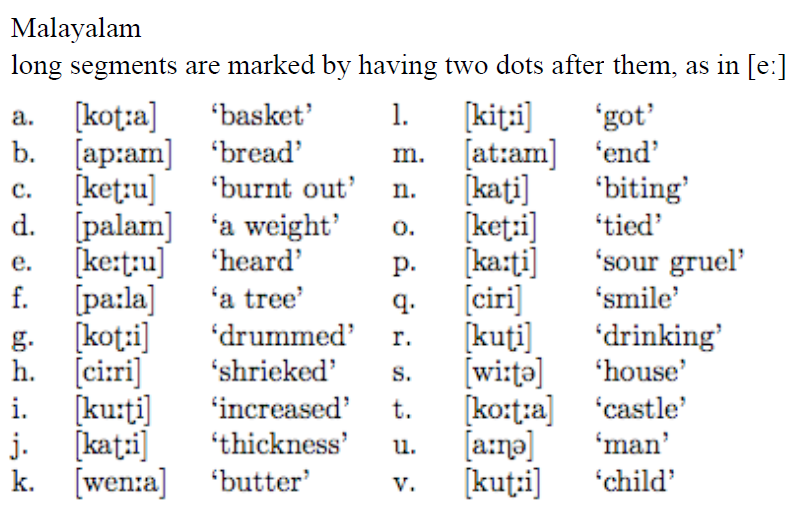
\includegraphics{../images/malayalam.png}
\end{figure}

~\\
INSTRUCTOR NOTES: Short and long vowels appear to be contrastive (phonemic) in Malayalam, as evidenced by minimal pairs that differ only in terms of their vowel length, such as [koʈːa] ‘basket’ vs. [koːʈːa] ‘castle’ or [keʈːu] ‘burnt out’ vs. [keːʈːu] ‘heard.’


\vfill
Excellent (3) ~~~ Good (2.2) ~~~ Fair (1.7) ~~~ Poor (0)
\newpage

\begin{center}
\textbf{{\color{red}{\HUGE END OF EXAM}}}\\

\end{center}
\newpage

\begin{center}
\textbf{{\color{blue}{\HUGE START OF EXAM\\}}}

\textbf{{\color{blue}{\HUGE Student ID: 16758\\}}}

\textbf{{\color{blue}{\HUGE \\}}}

\end{center}
\newpage

{\large Question 1}\\

Topic: Transcription\\
Source: Week 2 Handout, Part II, Question 3\\

Explain why people might legitimately disagree about how many sounds this particular word contains.\\

<better>


~\\
INSTRUCTOR NOTES: 


\vfill
Excellent (3) ~~~ Good (2.2) ~~~ Fair (1.7) ~~~ Poor (0)
\newpage

{\large Question 2}\\

Topic: Articulatory Phonetics\\
Source: Week 3 Handout, Question 13\\

Explain why this image does or does not match the description.\\

\begin{itemize} \item A one-handed sign. \item Location: At the signer’s nose. \item Handshape: Starts with index finger extended; finger folds down into a “hook” shape during the sign; then straightens and repeats the folding. \item Movement: No movement other than the change in handshape. \end{itemize}

\begin{figure}[H]
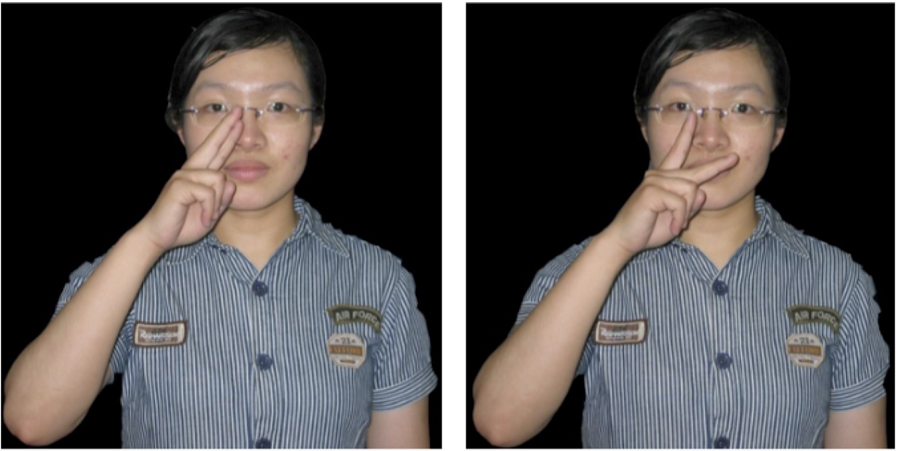
\includegraphics{../images/taiwansign_wrong.png}
\caption{WRONG}
\end{figure}

~\\
INSTRUCTOR NOTES: no; handshape is wrong


\vfill
Excellent (3) ~~~ Good (2.2) ~~~ Fair (1.7) ~~~ Poor (0)
\newpage

{\large Question 3}\\

Topic: Phonological Features\\
Source: Week 4 Discussion\\

Explain why phonological features are used instead of phonetic characteristics in analyzing datasets.\\


~\\
INSTRUCTOR NOTES: Phonological features help to capture phonological patterns, i.e., they group sounds together based on whether they do things like triggering a change or undergoing a change. Phonological features are sometimes language-specific. Phonetic characteristics are simply descriptions of the physical properties of the sounds; they are language-universal and independent of the patterns (though it turns out that many phonological patterns are based on phonetic characteristic groupings).


\vfill
Excellent (3) ~~~ Good (2.2) ~~~ Fair (1.7) ~~~ Poor (0)
\newpage

{\large Question 4}\\

Topic: Skewed Distributions\\
Source: Week 5 Handout, Question 3\\

What evidence is there that there is a pattern in these data, assuming that these are the only CV and VC sequences that occur in some language?\\

{[sa]}, {[ʃi]}, {[za]}, {[ʒi]}, {[as]}, {[iʃ]}, {[az]}, {[iʒ]}


~\\
INSTRUCTOR NOTES: (the palatal sounds occur with the high vowel, while the alveolar sounds occur with the low vowel)


\vfill
Excellent (3) ~~~ Good (2.2) ~~~ Fair (1.7) ~~~ Poor (0)
\newpage

{\large Question 5}\\

Topic: Phonological Relationships and Analysis\\
Source: Week 7 Handout, Question 9\\

What is the basic analysis of vowel length in this dataset, and what are the key pieces of evidence?\\

\begin{figure}[H]
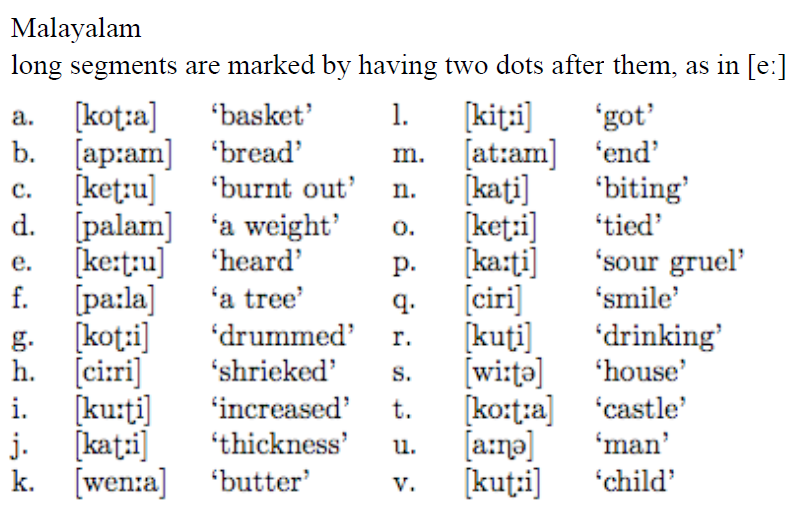
\includegraphics{../images/malayalam.png}
\end{figure}

~\\
INSTRUCTOR NOTES: Short and long vowels appear to be contrastive (phonemic) in Malayalam, as evidenced by minimal pairs that differ only in terms of their vowel length, such as [koʈːa] ‘basket’ vs. [koːʈːa] ‘castle’ or [keʈːu] ‘burnt out’ vs. [keːʈːu] ‘heard.’


\vfill
Excellent (3) ~~~ Good (2.2) ~~~ Fair (1.7) ~~~ Poor (0)
\newpage

\begin{center}
\textbf{{\color{red}{\HUGE END OF EXAM}}}\\

\end{center}
\newpage

\begin{center}
\textbf{{\color{blue}{\HUGE START OF EXAM\\}}}

\textbf{{\color{blue}{\HUGE Student ID: 16922\\}}}

\textbf{{\color{blue}{\HUGE \\}}}

\end{center}
\newpage

{\large Question 1}\\

Topic: Transcription\\
Source: Week 2 Handout, Part II, Question 11\\

How would this word be transcribed?\\ (Kathleen will then ask a follow-up question about your transcription.)\\

<bird>


~\\
INSTRUCTOR NOTES: [bɹ̩d]


\vfill
Excellent (3) ~~~ Good (2.2) ~~~ Fair (1.7) ~~~ Poor (0)
\newpage

{\large Question 2}\\

Topic: Articulatory Phonetics\\
Source: Week 3 Discussion\\

Describe what the tongue would do / where it would move during each of the vowels in this word.\\

<vacuum>


~\\
INSTRUCTOR NOTES: 


\vfill
Excellent (3) ~~~ Good (2.2) ~~~ Fair (1.7) ~~~ Poor (0)
\newpage

{\large Question 3}\\

Topic: Phonological Features\\
Source: Quiz 3, Question 12\\

Explain how you figure out which feature is involved in the process of umlaut shown below.\\

\begin{figure}[H]
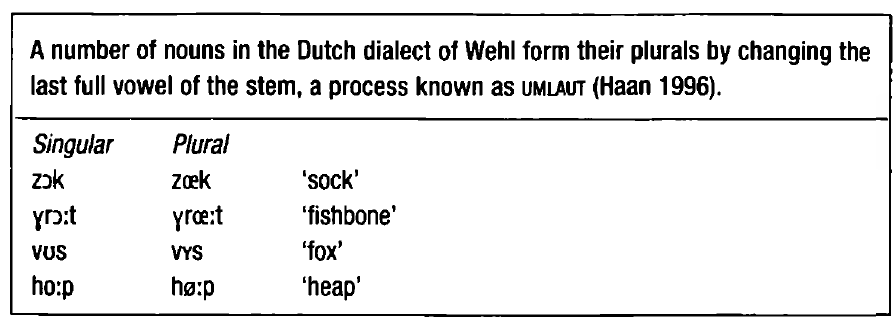
\includegraphics{../images/dutch.png}
\end{figure}

~\\
INSTRUCTOR NOTES: we look to see which vowels are affected, and compare them to see which feature is DIFFERENT (not e.g. what features they share); so since the vowels in the singular and plural are identical except that the singular forms are back and the plural are front, it's the feature [back] that is relevant / changing / involved (not e.g. the feature [round] just because all of the vowels are round)


\vfill
Excellent (3) ~~~ Good (2.2) ~~~ Fair (1.7) ~~~ Poor (0)
\newpage

{\large Question 4}\\

Topic: Skewed Distributions\\
Source: Quiz 4, Question 1\\

L$_X$ (Language X) has three vowels, [i], [a], and [u]. It has bi-syllabic roots like Kikuyu. It does not allow non-identical high vowels to co-occur. Of the following nine logically possible vocalic sequences, which ones should be unattested in L$_X$? Explain why.\\

\begin{itemize} \item {[i...i]} \item {[i...a]} \item {[i...u]} \item {[a...i]} \item {[a...a]} \item {[a...u]} \item {[u...i]} \item {[u...a]} \item {[u...u]} \end{itemize}


~\\
INSTRUCTOR NOTES: [i...u], [u...i]


\vfill
Excellent (3) ~~~ Good (2.2) ~~~ Fair (1.7) ~~~ Poor (0)
\newpage

{\large Question 5}\\

Topic: Phonological Relationships and Analysis\\
Source: Week 6 Handout, Question 11\\

What do the two signs below tell you about the phonological status of \underline{handshape} in ASL, and why?\\

\begin{figure}[H]
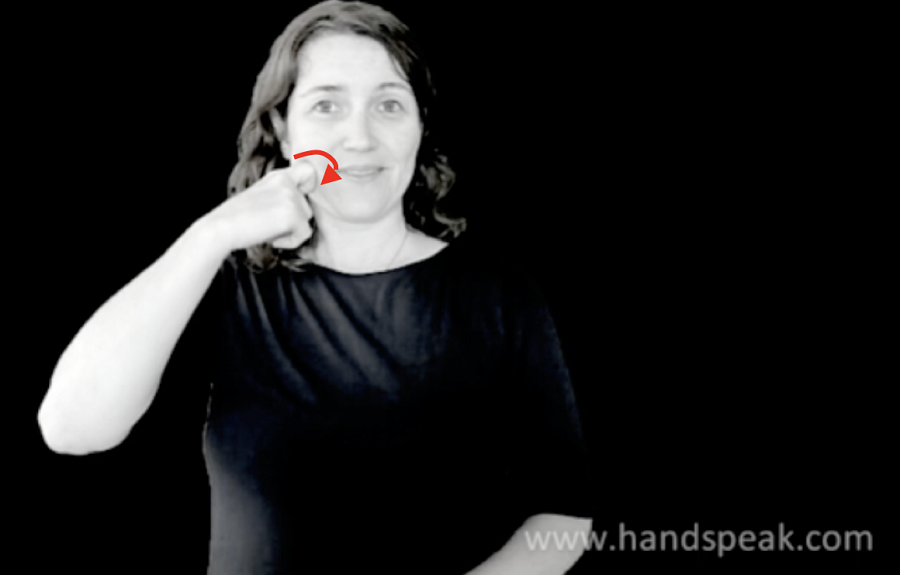
\includegraphics{../images/asl_apple.png}
\caption{APPLE}
\end{figure}
\begin{figure}[H]
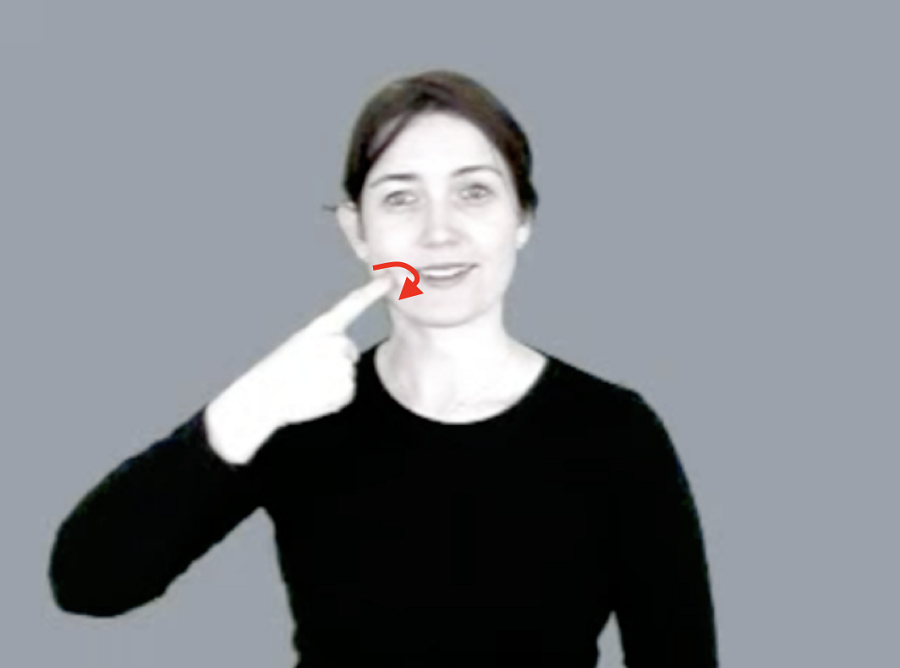
\includegraphics{../images/asl_candy.png}
\caption{CANDY}
\end{figure}

~\\
INSTRUCTOR NOTES: shows contrast because movement and location are same


\vfill
Excellent (3) ~~~ Good (2.2) ~~~ Fair (1.7) ~~~ Poor (0)
\newpage

\begin{center}
\textbf{{\color{red}{\HUGE END OF EXAM}}}\\

\end{center}
\newpage

\begin{center}
\textbf{{\color{blue}{\HUGE START OF EXAM\\}}}

\textbf{{\color{blue}{\HUGE Student ID: 17335\\}}}

\textbf{{\color{blue}{\HUGE \\}}}

\end{center}
\newpage

{\large Question 1}\\

Topic: Transcription\\
Source: Week 2 Handout, Part II, Question 11\\

How would this word be transcribed?\\ (Kathleen will then ask a follow-up question about your transcription.)\\

<wealth>


~\\
INSTRUCTOR NOTES: [wɛlθ]


\vfill
Excellent (3) ~~~ Good (2.2) ~~~ Fair (1.7) ~~~ Poor (0)
\newpage

{\large Question 2}\\

Topic: Articulatory Phonetics\\
Source: Week 3 Discussion\\

Describe what the tongue would do / where it would move during each of the vowels in this word.\\

<follow>


~\\
INSTRUCTOR NOTES: 


\vfill
Excellent (3) ~~~ Good (2.2) ~~~ Fair (1.7) ~~~ Poor (0)
\newpage

{\large Question 3}\\

Topic: Phonological Features\\
Source: Quiz 3, Question 12\\

Explain how you figure out which feature is involved in the process of umlaut shown below.\\

\begin{figure}[H]
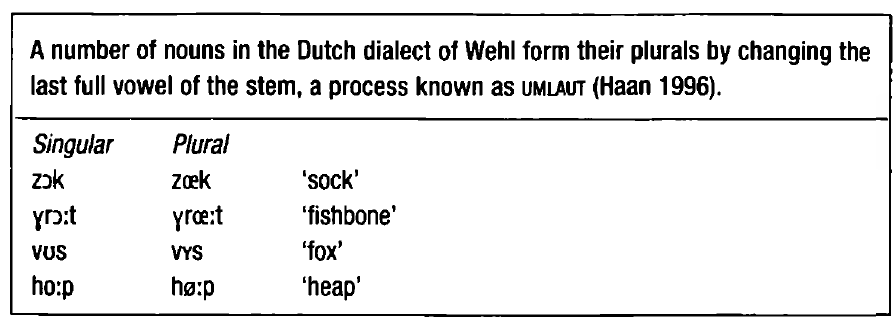
\includegraphics{../images/dutch.png}
\end{figure}

~\\
INSTRUCTOR NOTES: we look to see which vowels are affected, and compare them to see which feature is DIFFERENT (not e.g. what features they share); so since the vowels in the singular and plural are identical except that the singular forms are back and the plural are front, it's the feature [back] that is relevant / changing / involved (not e.g. the feature [round] just because all of the vowels are round)


\vfill
Excellent (3) ~~~ Good (2.2) ~~~ Fair (1.7) ~~~ Poor (0)
\newpage

{\large Question 4}\\

Topic: Skewed Distributions\\
Source: Quiz 4, Question 2\\

L$_X$ (Language X) has three vowels, [i], [a], and [u]. L$_X$ has tri-syllabic roots. If L$_X$ does not allow non-identical high vowels to co-occur, which one of the following tri-syllabic vocalic sequences do you predict to be unattested in L$_X$? Explain why.\\

\begin{itemize} \item {[u...i...a]} \item {[a...i...a]} \item {[u...u...a]} \item {[a...i...i]} \end{itemize}


~\\
INSTRUCTOR NOTES: [u...i...a]


\vfill
Excellent (3) ~~~ Good (2.2) ~~~ Fair (1.7) ~~~ Poor (0)
\newpage

{\large Question 5}\\

Topic: Phonological Relationships and Analysis\\
Source: Week 7 Handout, Question 12\\

What is the basic analysis of oral and nasal vowels in this dataset, and what are the key pieces of evidence?\\

\begin{figure}[H]
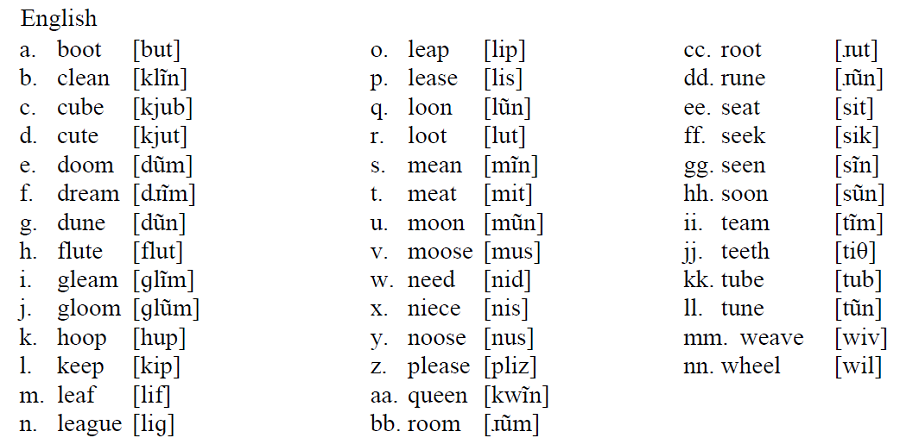
\includegraphics{../images/english12.png}
\end{figure}

~\\
INSTRUCTOR NOTES: The pairs of sounds [i] and [ĩ], and [u] and [ũ], are each allophonic and therefore allophones of the same phoneme in English (though the two pairs represent two contrastive phonemes in English). The sounds [i] and [ĩ] are in complementary distribution in English, with [ĩ] occurring before the sounds [m] and [n], (e.g., [ɡlĩm] ‘gleam’ and [klĩn] ‘clean’) and [i] occurring elsewhere (e.g., [lip] ‘leap’). Similarly, the sounds [u] and [ũ] are also in complementary distribution, with exactly the same conditioning environments: [ũ] occurs before [m] and [n] (e.g., [dũm] ‘doom’ and [dũn] ‘dune’), and [u] occurs elsewhere (e.g. [but] ‘boot’). Thus, within each pair, we treat the vowels as allophonic. 


\vfill
Excellent (3) ~~~ Good (2.2) ~~~ Fair (1.7) ~~~ Poor (0)
\newpage

\begin{center}
\textbf{{\color{red}{\HUGE END OF EXAM}}}\\

\end{center}
\newpage

\begin{center}
\textbf{{\color{blue}{\HUGE START OF EXAM\\}}}

\textbf{{\color{blue}{\HUGE Student ID: 17357\\}}}

\textbf{{\color{blue}{\HUGE \\}}}

\end{center}
\newpage

{\large Question 1}\\

Topic: Transcription\\
Source: Week 2 Handout, Part II, Question 11\\

How would this word be transcribed?\\ (Kathleen will then ask a follow-up question about your transcription.)\\

<segment>


~\\
INSTRUCTOR NOTES: [sɛɡmɛnt]


\vfill
Excellent (3) ~~~ Good (2.2) ~~~ Fair (1.7) ~~~ Poor (0)
\newpage

{\large Question 2}\\

Topic: Articulatory Phonetics\\
Source: Week 3 Handout, Question 7\\

Is the symbol given a reasonable way to transcribe any of the sounds described below? If so, which one? If not, why not? Explain your answer.\\

{[ʒ]}

\begin{itemize} \item voiceless palatal affricate \item voiced velar nasal \item voiceless glottal fricative \item voiced labiodental fricative \item voiced interdental fricative \item voiced palatal fricative \end{itemize}


~\\
INSTRUCTOR NOTES: yes (voiced palatal fricative)


\vfill
Excellent (3) ~~~ Good (2.2) ~~~ Fair (1.7) ~~~ Poor (0)
\newpage

{\large Question 3}\\

Topic: Phonological Features\\
Source: Week 4 Discussion\\

Explain what the given feature’s value is for this class of sounds, and why.\\

{[LABIAL]}

interdentals


~\\
INSTRUCTOR NOTES: 0, because interdentals aren't [LABIAL], but [LABIAL] is monovalent, so they're not [-labial]


\vfill
Excellent (3) ~~~ Good (2.2) ~~~ Fair (1.7) ~~~ Poor (0)
\newpage

{\large Question 4}\\

Topic: Skewed Distributions\\
Source: Week 5 Handout, Question 5\\

Explain why looking for patterns with consonants and vowels is a more reasonable approach to pattern finding in this dataset than looking for patterns with respect to all of the individual sounds in Ukrainian.\\

\begin{figure}[H]
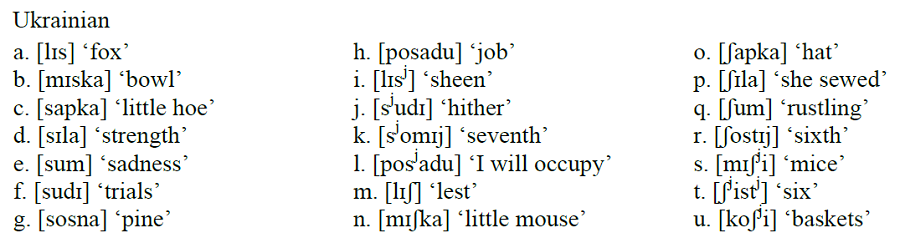
\includegraphics{../images/ukrainian.png}
\end{figure}

~\\
INSTRUCTOR NOTES: Collapsing sounds into "consonants" and "vowels" allows us to have 'sufficient data' in a way that thinking about all the individual combinations of sounds would not.


\vfill
Excellent (3) ~~~ Good (2.2) ~~~ Fair (1.7) ~~~ Poor (0)
\newpage

{\large Question 5}\\

Topic: Phonological Relationships and Analysis\\
Source: Week 6 Handout, Question 11\\

What do the two signs below tell you about the phonological status of \underline{handshape} in ASL, and why?\\

\begin{figure}[H]
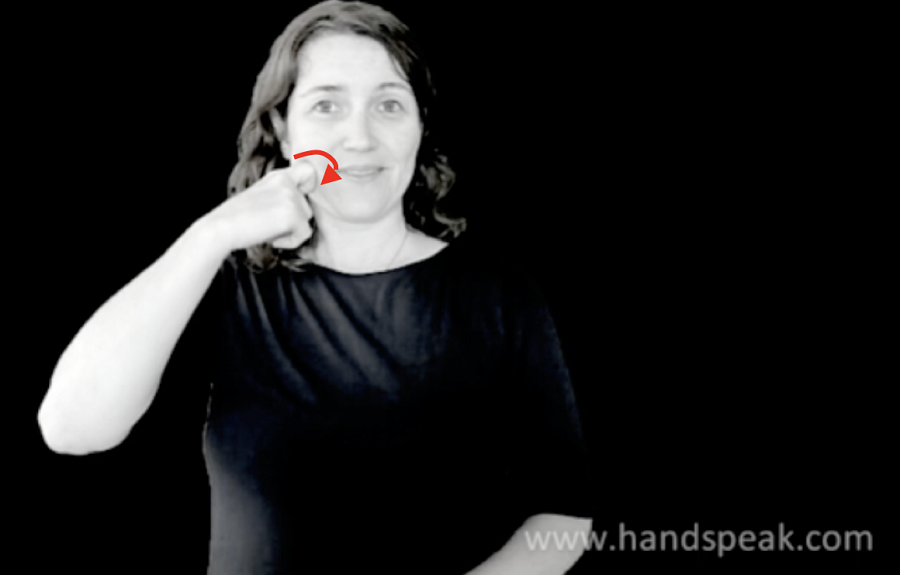
\includegraphics{../images/asl_apple.png}
\caption{APPLE}
\end{figure}
\begin{figure}[H]
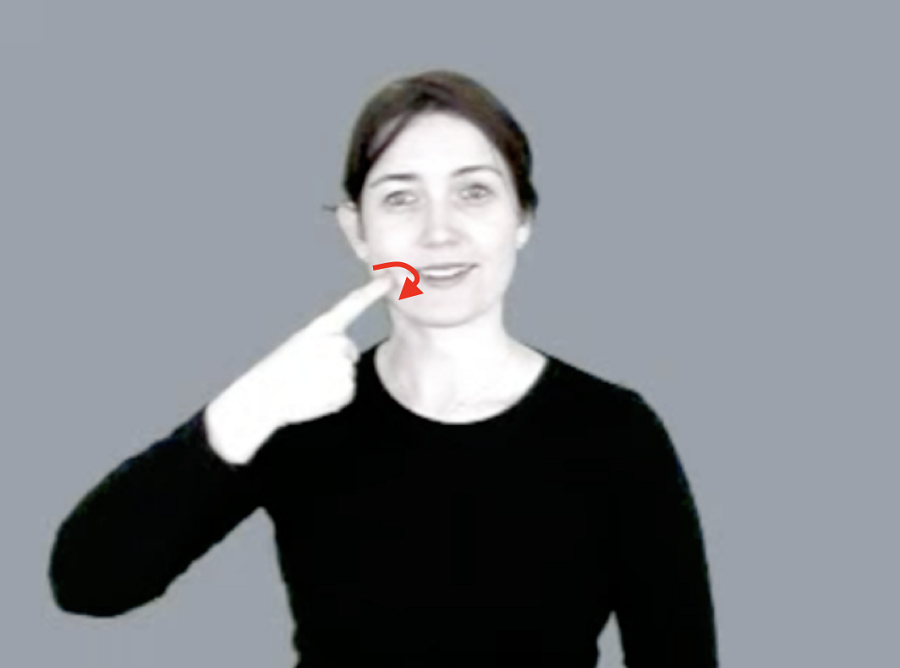
\includegraphics{../images/asl_candy.png}
\caption{CANDY}
\end{figure}

~\\
INSTRUCTOR NOTES: shows contrast because movement and location are same


\vfill
Excellent (3) ~~~ Good (2.2) ~~~ Fair (1.7) ~~~ Poor (0)
\newpage

\begin{center}
\textbf{{\color{red}{\HUGE END OF EXAM}}}\\

\end{center}
\newpage

\begin{center}
\textbf{{\color{blue}{\HUGE START OF EXAM\\}}}

\textbf{{\color{blue}{\HUGE Student ID: 17359\\}}}

\textbf{{\color{blue}{\HUGE \\}}}

\end{center}
\newpage

{\large Question 1}\\

Topic: Transcription\\
Source: Quiz 1, Question 10\\

Explain whether this word either does or does not have an [ʃ] sound in it, and why the spelling and pronunciation either do or do not align.\\

<bassoon>


~\\
INSTRUCTOR NOTES: 


\vfill
Excellent (3) ~~~ Good (2.2) ~~~ Fair (1.7) ~~~ Poor (0)
\newpage

{\large Question 2}\\

Topic: Articulatory Phonetics\\
Source: Week 3 Discussion\\

Assuming a Standard North American English inventory, does this vowel need to have tenseness specified if you're giving a prose description? Why or why not?\\

{[ɑ]}


~\\
INSTRUCTOR NOTES: no


\vfill
Excellent (3) ~~~ Good (2.2) ~~~ Fair (1.7) ~~~ Poor (0)
\newpage

{\large Question 3}\\

Topic: Phonological Features\\
Source: Quiz 3, Question 12\\

Explain how you figure out which feature is involved in the process of umlaut shown below.\\

\begin{figure}[H]
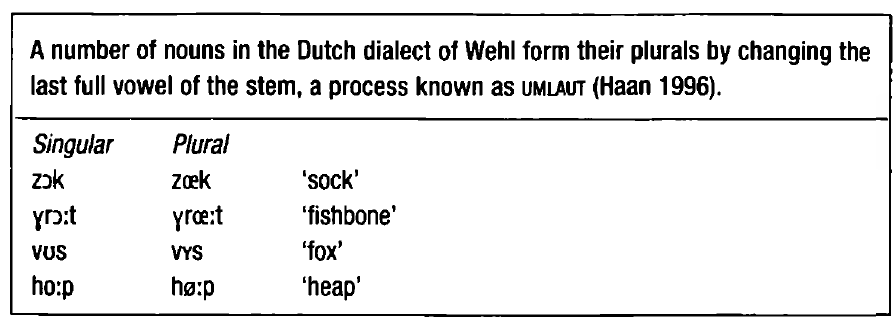
\includegraphics{../images/dutch.png}
\end{figure}

~\\
INSTRUCTOR NOTES: we look to see which vowels are affected, and compare them to see which feature is DIFFERENT (not e.g. what features they share); so since the vowels in the singular and plural are identical except that the singular forms are back and the plural are front, it's the feature [back] that is relevant / changing / involved (not e.g. the feature [round] just because all of the vowels are round)


\vfill
Excellent (3) ~~~ Good (2.2) ~~~ Fair (1.7) ~~~ Poor (0)
\newpage

{\large Question 4}\\

Topic: Skewed Distributions\\
Source: Week 5 Handout, Question 1\\

Explain why we think that languages are not random in terms of their phonology.\\


~\\
INSTRUCTOR NOTES: 


\vfill
Excellent (3) ~~~ Good (2.2) ~~~ Fair (1.7) ~~~ Poor (0)
\newpage

{\large Question 5}\\

Topic: Phonological Relationships and Analysis\\
Source: Week 7 Handout, Question 12\\

What is the basic analysis of oral and nasal vowels in this dataset, and what are the key pieces of evidence?\\

\begin{figure}[H]
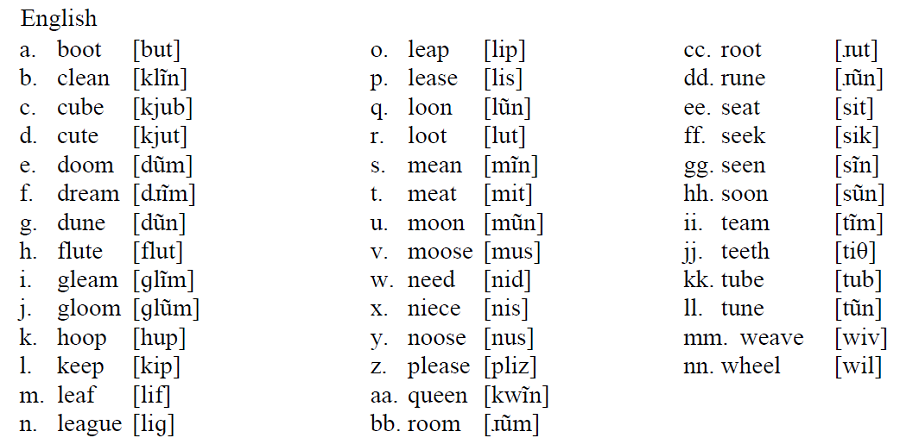
\includegraphics{../images/english12.png}
\end{figure}

~\\
INSTRUCTOR NOTES: The pairs of sounds [i] and [ĩ], and [u] and [ũ], are each allophonic and therefore allophones of the same phoneme in English (though the two pairs represent two contrastive phonemes in English). The sounds [i] and [ĩ] are in complementary distribution in English, with [ĩ] occurring before the sounds [m] and [n], (e.g., [ɡlĩm] ‘gleam’ and [klĩn] ‘clean’) and [i] occurring elsewhere (e.g., [lip] ‘leap’). Similarly, the sounds [u] and [ũ] are also in complementary distribution, with exactly the same conditioning environments: [ũ] occurs before [m] and [n] (e.g., [dũm] ‘doom’ and [dũn] ‘dune’), and [u] occurs elsewhere (e.g. [but] ‘boot’). Thus, within each pair, we treat the vowels as allophonic. 


\vfill
Excellent (3) ~~~ Good (2.2) ~~~ Fair (1.7) ~~~ Poor (0)
\newpage

\begin{center}
\textbf{{\color{red}{\HUGE END OF EXAM}}}\\

\end{center}
\newpage

\begin{center}
\textbf{{\color{blue}{\HUGE START OF EXAM\\}}}

\textbf{{\color{blue}{\HUGE Student ID: 17393\\}}}

\textbf{{\color{blue}{\HUGE \\}}}

\end{center}
\newpage

{\large Question 1}\\

Topic: Transcription\\
Source: Week 2 Handout, Part II\\

Is this a reasonable transcription of this word? Explain why.\\

<mouse>: {[mɔɪs]}


~\\
INSTRUCTOR NOTES: no, [ɑʊ]


\vfill
Excellent (3) ~~~ Good (2.2) ~~~ Fair (1.7) ~~~ Poor (0)
\newpage

{\large Question 2}\\

Topic: Articulatory Phonetics\\
Source: Quiz 2, Question 6\\

In the pronunciation of this word, which sounds are obstruents and which are sonorants? Explain your answer.\\

<fricative>


~\\
INSTRUCTOR NOTES: [fɹɪkətɪv] -- sonorants: [ɹɪəɪ] and obstruents: [fktv]


\vfill
Excellent (3) ~~~ Good (2.2) ~~~ Fair (1.7) ~~~ Poor (0)
\newpage

{\large Question 3}\\

Topic: Phonological Features\\
Source: Quiz 3, Question 3\\

Explain why this featural specification either does or does not match the given sound.\\

{[+consonantal]}, {[-sonorant]}

{[f]}


~\\
INSTRUCTOR NOTES: matches


\vfill
Excellent (3) ~~~ Good (2.2) ~~~ Fair (1.7) ~~~ Poor (0)
\newpage

{\large Question 4}\\

Topic: Skewed Distributions\\
Source: Week 5 Handout, Question 6\\

What would be a good description of the pattern in Malto? What characteristics make that a good description?\\

\begin{figure}[H]
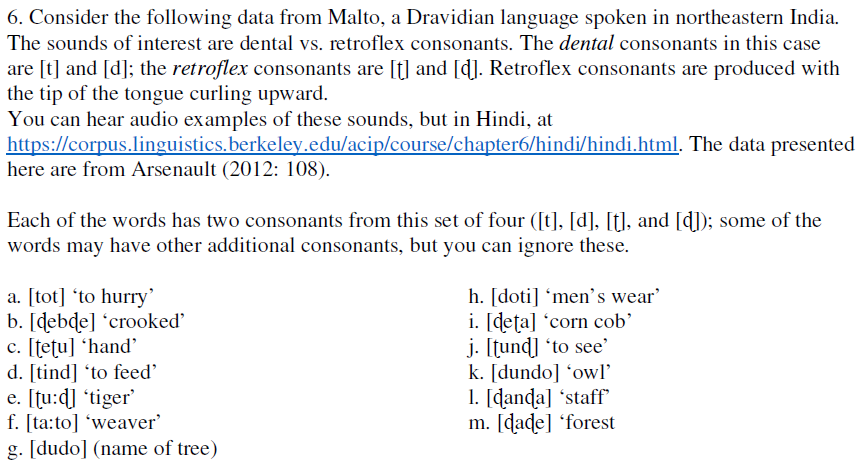
\includegraphics{../images/malto.png}
\end{figure}

~\\
INSTRUCTOR NOTES: It is not possible to have stops of different places of articulation co-occurring in a single word. Instead, if there are two stops, both must be dental, or both must be retroflex. For example, it’s possible to have a word with two dental stops, as in [tot] ‘to hurry’ (even if they disagree in voicing, as in [tind] ‘to feed’), or a word with two retroflex stops, as in [ɖebɖe] ‘crooked’ (again, regardless of voicing, as in [ɖeʈa] ‘corn cob’). But there are no words that have one dental and one retroflex stop, in either order, regardless of voicing. (accurate, generalizations, concrete examples)


\vfill
Excellent (3) ~~~ Good (2.2) ~~~ Fair (1.7) ~~~ Poor (0)
\newpage

{\large Question 5}\\

Topic: Phonological Relationships and Analysis\\
Source: Week 6 Handout, Question 11\\

What do the two signs below tell you about the phonological status of \underline{handshape} in ASL, and why?\\

\begin{figure}[H]
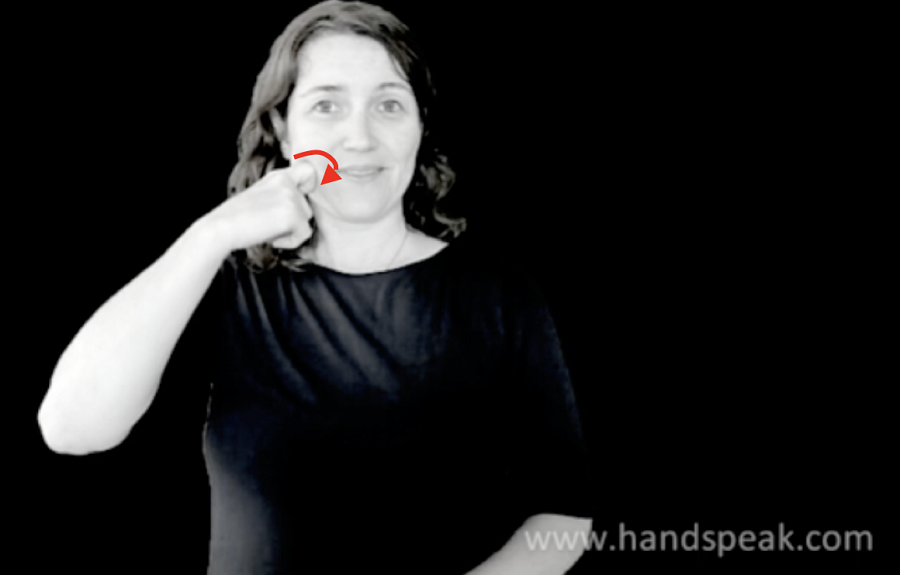
\includegraphics{../images/asl_apple.png}
\caption{APPLE}
\end{figure}
\begin{figure}[H]
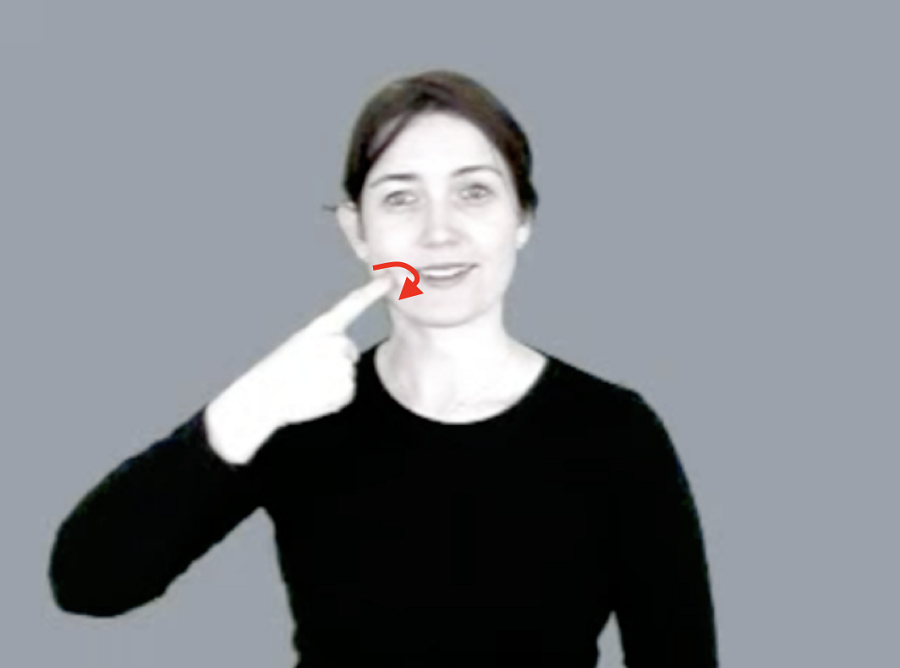
\includegraphics{../images/asl_candy.png}
\caption{CANDY}
\end{figure}

~\\
INSTRUCTOR NOTES: shows contrast because movement and location are same


\vfill
Excellent (3) ~~~ Good (2.2) ~~~ Fair (1.7) ~~~ Poor (0)
\newpage

\begin{center}
\textbf{{\color{red}{\HUGE END OF EXAM}}}\\

\end{center}
\newpage

\begin{center}
\textbf{{\color{blue}{\HUGE START OF EXAM\\}}}

\textbf{{\color{blue}{\HUGE Student ID: 17487\\}}}

\textbf{{\color{blue}{\HUGE \\}}}

\end{center}
\newpage

{\large Question 1}\\

Topic: Transcription\\
Source: Week 2 Handout, Part II, Question 3\\

Explain why people might legitimately disagree about how many sounds this particular word contains.\\

<better>


~\\
INSTRUCTOR NOTES: 


\vfill
Excellent (3) ~~~ Good (2.2) ~~~ Fair (1.7) ~~~ Poor (0)
\newpage

{\large Question 2}\\

Topic: Articulatory Phonetics\\
Source: Week 3 Discussion\\

Describe what the tongue would do / where it would move during each of the vowels in this word.\\

<bookmark>


~\\
INSTRUCTOR NOTES: 


\vfill
Excellent (3) ~~~ Good (2.2) ~~~ Fair (1.7) ~~~ Poor (0)
\newpage

{\large Question 3}\\

Topic: Phonological Features\\
Source: Week 4 Discussion\\

Explain what the given feature’s value is for this class of sounds, and why.\\

{[consonantal]}

glides


~\\
INSTRUCTOR NOTES: [-], because the constriction isn't as narrow as it would be for a fricative


\vfill
Excellent (3) ~~~ Good (2.2) ~~~ Fair (1.7) ~~~ Poor (0)
\newpage

{\large Question 4}\\

Topic: Skewed Distributions\\
Source: Week 5 Handout, Question 6\\

If I gave you a new word in Malto, [di\_\_u], would it be possible to predict whether it's [d] or [t] that goes in the blank? Explain why or why not.\\

\begin{figure}[H]
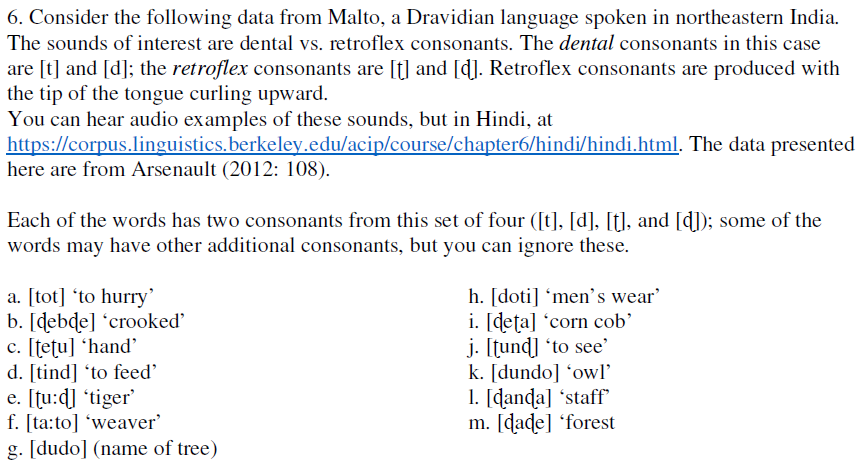
\includegraphics{../images/malto.png}
\end{figure}

~\\
INSTRUCTOR NOTES: No, it's not possible. In Malto, you can predict that there are two dental or two retroflex stops in a word, but you can't predict the voicing. These two sounds are both dental, so there's no way to predict.


\vfill
Excellent (3) ~~~ Good (2.2) ~~~ Fair (1.7) ~~~ Poor (0)
\newpage

{\large Question 5}\\

Topic: Phonological Relationships and Analysis\\
Source: Week 6 Handout, Question 11\\

What do the two signs below tell you about the phonological status of \underline{handshape} in ASL, and why?\\

\begin{figure}[H]
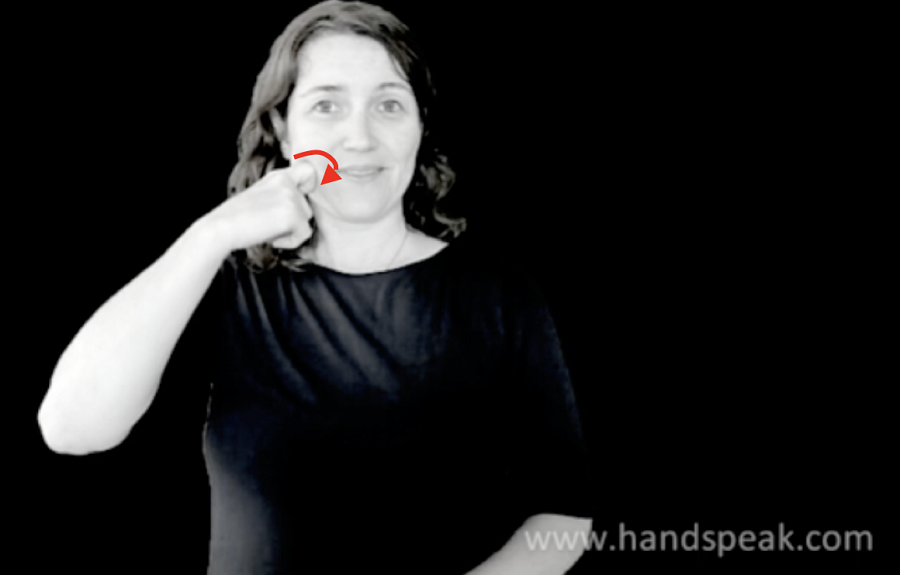
\includegraphics{../images/asl_apple.png}
\caption{APPLE}
\end{figure}
\begin{figure}[H]
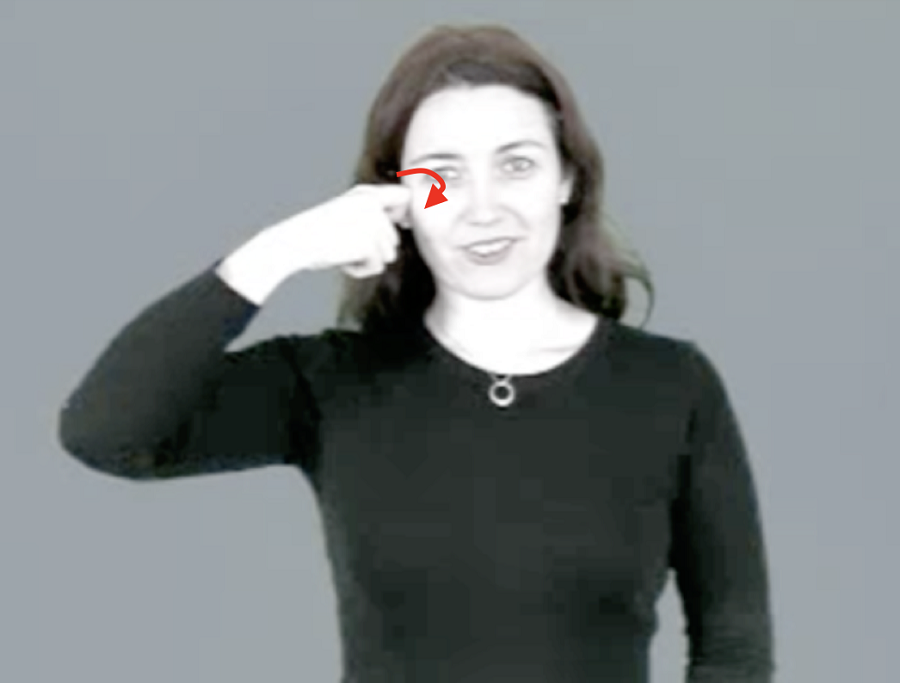
\includegraphics{../images/asl_onion.png}
\caption{ONION}
\end{figure}

~\\
INSTRUCTOR NOTES: shows contrast, because handshape and movement are the same


\vfill
Excellent (3) ~~~ Good (2.2) ~~~ Fair (1.7) ~~~ Poor (0)
\newpage

\begin{center}
\textbf{{\color{red}{\HUGE END OF EXAM}}}\\

\end{center}
\newpage

\begin{center}
\textbf{{\color{blue}{\HUGE START OF EXAM\\}}}

\textbf{{\color{blue}{\HUGE Student ID: 18870\\}}}

\textbf{{\color{blue}{\HUGE \\}}}

\end{center}
\newpage

{\large Question 1}\\

Topic: Transcription\\
Source: Week 2 Handout, Part II, Question 11\\

How would this word be transcribed?\\ (Kathleen will then ask a follow-up question about your transcription.)\\

<nice>


~\\
INSTRUCTOR NOTES: [nɑɪs]


\vfill
Excellent (3) ~~~ Good (2.2) ~~~ Fair (1.7) ~~~ Poor (0)
\newpage

{\large Question 2}\\

Topic: Articulatory Phonetics\\
Source: Week 3 Discussion\\

Describe what the tongue would do / where it would move during each of the vowels in this word.\\

<vacuum>


~\\
INSTRUCTOR NOTES: 


\vfill
Excellent (3) ~~~ Good (2.2) ~~~ Fair (1.7) ~~~ Poor (0)
\newpage

{\large Question 3}\\

Topic: Phonological Features\\
Source: Week 4 Discussion\\

Explain what the given feature’s value is for this class of sounds, and why.\\

{[LABIAL]}

interdentals


~\\
INSTRUCTOR NOTES: 0, because interdentals aren't [LABIAL], but [LABIAL] is monovalent, so they're not [-labial]


\vfill
Excellent (3) ~~~ Good (2.2) ~~~ Fair (1.7) ~~~ Poor (0)
\newpage

{\large Question 4}\\

Topic: Skewed Distributions\\
Source: Week 5 Handout, Question 6\\

If I gave you a new word in Malto, [di\_\_u], would it be possible to predict whether it's [d] or [ɖ] that goes in the blank? Explain why or why not.\\

\begin{figure}[H]
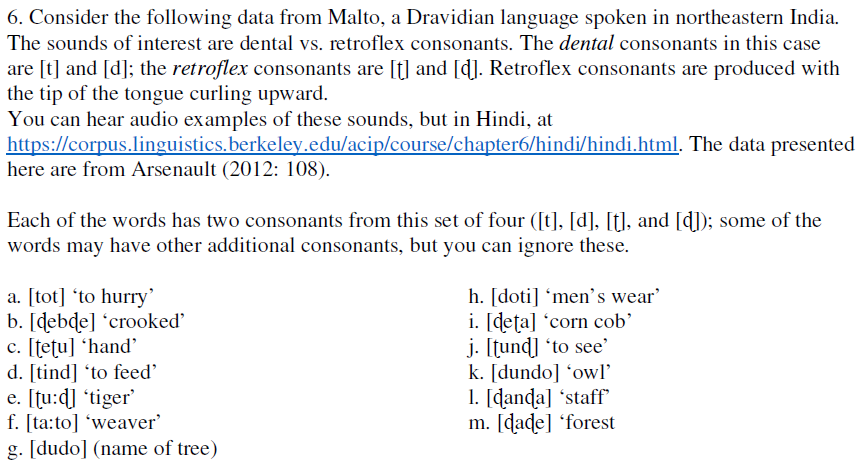
\includegraphics{../images/malto.png}
\end{figure}

~\\
INSTRUCTOR NOTES: Yes, it's possible; in Malto, if there are two stops in a word, they must either both be dental or both retroflex. Since the first sound is dental, the second must also be dental (though to be fair, you couldn't actually predict that it's [d] and not [t], but the question restricts it to only the voiced options).


\vfill
Excellent (3) ~~~ Good (2.2) ~~~ Fair (1.7) ~~~ Poor (0)
\newpage

{\large Question 5}\\

Topic: Phonological Relationships and Analysis\\
Source: Week 6 Handout, Question 11\\

What do the two signs below tell you about the phonological status of \underline{handshape} in ASL, and why?\\

\begin{figure}[H]
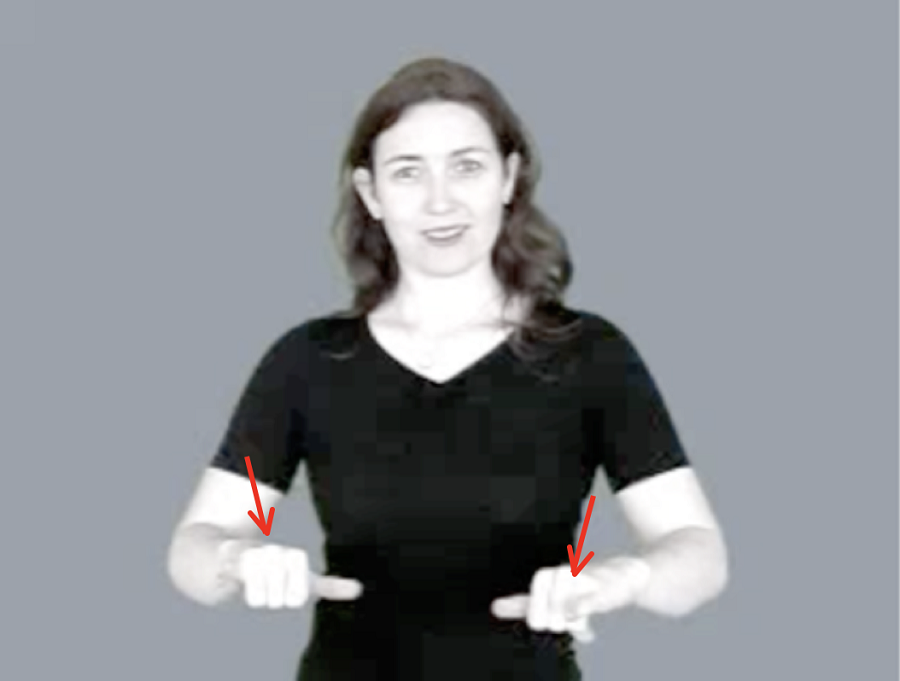
\includegraphics{../images/asl_stay.png}
\caption{STAY}
\end{figure}
\begin{figure}[H]
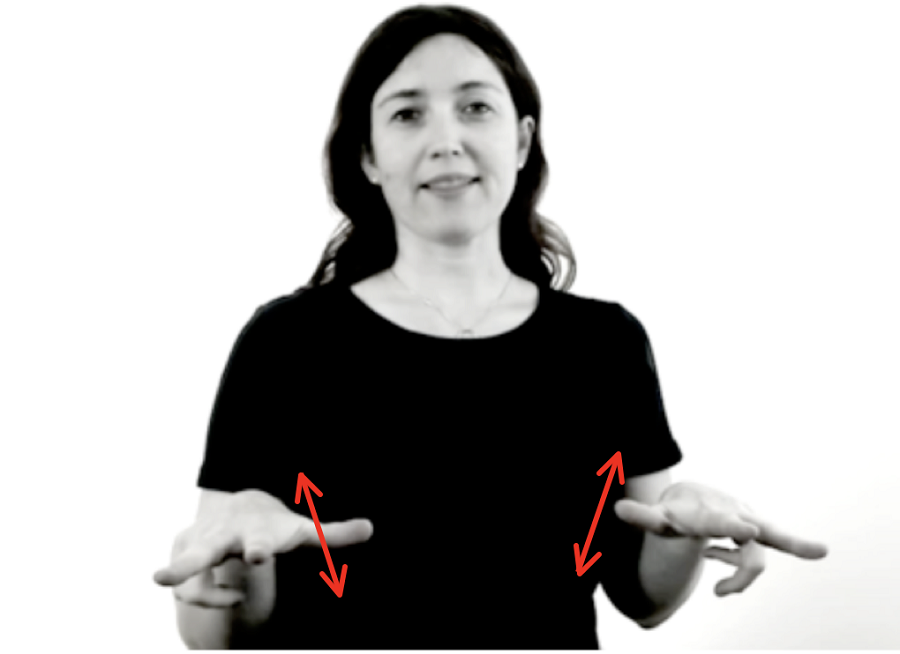
\includegraphics{../images/asl_awkward.png}
\caption{AWKWARD}
\end{figure}

~\\
INSTRUCTOR NOTES: nothing, because both handshape and movement are different


\vfill
Excellent (3) ~~~ Good (2.2) ~~~ Fair (1.7) ~~~ Poor (0)
\newpage

\begin{center}
\textbf{{\color{red}{\HUGE END OF EXAM}}}\\

\end{center}
\newpage

\begin{center}
\textbf{{\color{blue}{\HUGE START OF EXAM\\}}}

\textbf{{\color{blue}{\HUGE Student ID: 19086\\}}}

\textbf{{\color{blue}{\HUGE \\}}}

\end{center}
\newpage

{\large Question 1}\\

Topic: Transcription\\
Source: Week 2 Handout, Part II, Question 11\\

How would this word be transcribed?\\ (Kathleen will then ask a follow-up question about your transcription.)\\

<bird>


~\\
INSTRUCTOR NOTES: [bɹ̩d]


\vfill
Excellent (3) ~~~ Good (2.2) ~~~ Fair (1.7) ~~~ Poor (0)
\newpage

{\large Question 2}\\

Topic: Articulatory Phonetics\\
Source: Homework 1, Question 3(a)\\

Could this image be the result of producing the sound represented by the given IPA symbol? Why or why not?\\

{[n]}

\begin{figure}[H]
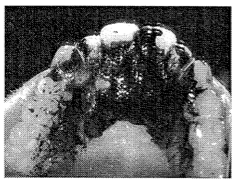
\includegraphics{../images/staticpalatography_stop.png}
\end{figure}

~\\
INSTRUCTOR NOTES: yes


\vfill
Excellent (3) ~~~ Good (2.2) ~~~ Fair (1.7) ~~~ Poor (0)
\newpage

{\large Question 3}\\

Topic: Phonological Features\\
Source: Week 4 Discussion\\

Explain why the given feature's value varies across this set of sounds.\\

{[voice]}

glottalized obstruents


~\\
INSTRUCTOR NOTES: includes both voiced and voiceless glottalized obstruents -- obs. can themselves be voiced or voiceless


\vfill
Excellent (3) ~~~ Good (2.2) ~~~ Fair (1.7) ~~~ Poor (0)
\newpage

{\large Question 4}\\

Topic: Skewed Distributions\\
Source: Week 5 Handout, Question 6\\

What would be a good description of the pattern in Malto? What characteristics make that a good description?\\

\begin{figure}[H]
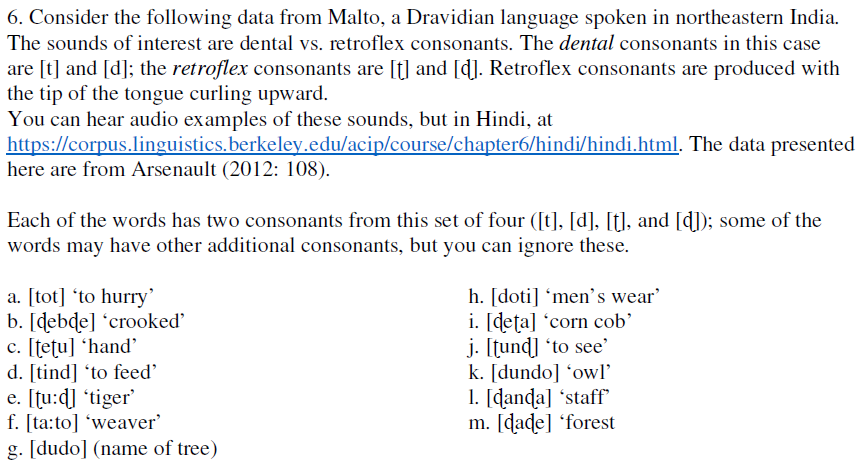
\includegraphics{../images/malto.png}
\end{figure}

~\\
INSTRUCTOR NOTES: It is not possible to have stops of different places of articulation co-occurring in a single word. Instead, if there are two stops, both must be dental, or both must be retroflex. For example, it’s possible to have a word with two dental stops, as in [tot] ‘to hurry’ (even if they disagree in voicing, as in [tind] ‘to feed’), or a word with two retroflex stops, as in [ɖebɖe] ‘crooked’ (again, regardless of voicing, as in [ɖeʈa] ‘corn cob’). But there are no words that have one dental and one retroflex stop, in either order, regardless of voicing. (accurate, generalizations, concrete examples)


\vfill
Excellent (3) ~~~ Good (2.2) ~~~ Fair (1.7) ~~~ Poor (0)
\newpage

{\large Question 5}\\

Topic: Phonological Relationships and Analysis\\
Source: Week 7 Handout, Question 12\\

What is the basic analysis of oral and nasal vowels in this dataset, and what are the key pieces of evidence?\\

\begin{figure}[H]
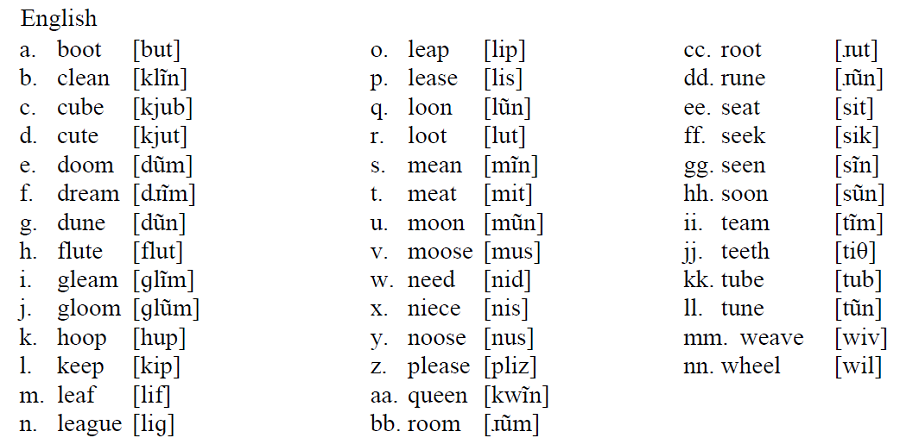
\includegraphics{../images/english12.png}
\end{figure}

~\\
INSTRUCTOR NOTES: The pairs of sounds [i] and [ĩ], and [u] and [ũ], are each allophonic and therefore allophones of the same phoneme in English (though the two pairs represent two contrastive phonemes in English). The sounds [i] and [ĩ] are in complementary distribution in English, with [ĩ] occurring before the sounds [m] and [n], (e.g., [ɡlĩm] ‘gleam’ and [klĩn] ‘clean’) and [i] occurring elsewhere (e.g., [lip] ‘leap’). Similarly, the sounds [u] and [ũ] are also in complementary distribution, with exactly the same conditioning environments: [ũ] occurs before [m] and [n] (e.g., [dũm] ‘doom’ and [dũn] ‘dune’), and [u] occurs elsewhere (e.g. [but] ‘boot’). Thus, within each pair, we treat the vowels as allophonic. 


\vfill
Excellent (3) ~~~ Good (2.2) ~~~ Fair (1.7) ~~~ Poor (0)
\newpage

\begin{center}
\textbf{{\color{red}{\HUGE END OF EXAM}}}\\

\end{center}
\newpage

\begin{center}
\textbf{{\color{blue}{\HUGE START OF EXAM\\}}}

\textbf{{\color{blue}{\HUGE Student ID: 19711\\}}}

\textbf{{\color{blue}{\HUGE \\}}}

\end{center}
\newpage

{\large Question 1}\\

Topic: Transcription\\
Source: Week 2 Handout, Part II\\

Is this a reasonable transcription of this word? Explain why.\\

<wimp>: {[wimp]}


~\\
INSTRUCTOR NOTES: no, [ɪ]


\vfill
Excellent (3) ~~~ Good (2.2) ~~~ Fair (1.7) ~~~ Poor (0)
\newpage

{\large Question 2}\\

Topic: Articulatory Phonetics\\
Source: Week 3 Discussion\\

Describe what the tongue would do / where it would move during each of the vowels in this word.\\

<puny>


~\\
INSTRUCTOR NOTES: 


\vfill
Excellent (3) ~~~ Good (2.2) ~~~ Fair (1.7) ~~~ Poor (0)
\newpage

{\large Question 3}\\

Topic: Phonological Features\\
Source: Week 4 Discussion\\

Explain what the given feature’s value is for this class of sounds, and why.\\

{[continuant]}

glottals


~\\
INSTRUCTOR NOTES: 0, because there is no constriction in the vocal tract for manner features to apply


\vfill
Excellent (3) ~~~ Good (2.2) ~~~ Fair (1.7) ~~~ Poor (0)
\newpage

{\large Question 4}\\

Topic: Skewed Distributions\\
Source: Week 5 Handout, Question 6\\

What would be a good description of the pattern in Malto? What characteristics make that a good description?\\

\begin{figure}[H]
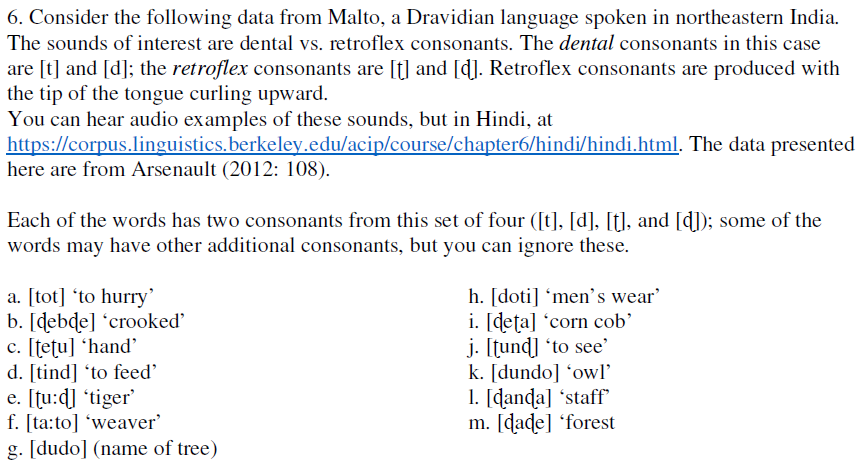
\includegraphics{../images/malto.png}
\end{figure}

~\\
INSTRUCTOR NOTES: It is not possible to have stops of different places of articulation co-occurring in a single word. Instead, if there are two stops, both must be dental, or both must be retroflex. For example, it’s possible to have a word with two dental stops, as in [tot] ‘to hurry’ (even if they disagree in voicing, as in [tind] ‘to feed’), or a word with two retroflex stops, as in [ɖebɖe] ‘crooked’ (again, regardless of voicing, as in [ɖeʈa] ‘corn cob’). But there are no words that have one dental and one retroflex stop, in either order, regardless of voicing. (accurate, generalizations, concrete examples)


\vfill
Excellent (3) ~~~ Good (2.2) ~~~ Fair (1.7) ~~~ Poor (0)
\newpage

{\large Question 5}\\

Topic: Phonological Relationships and Analysis\\
Source: Week 6 Handout, Question 11\\

What do the two signs below tell you about the phonological status of \underline{handshape} in ASL, and why?\\

\begin{figure}[H]
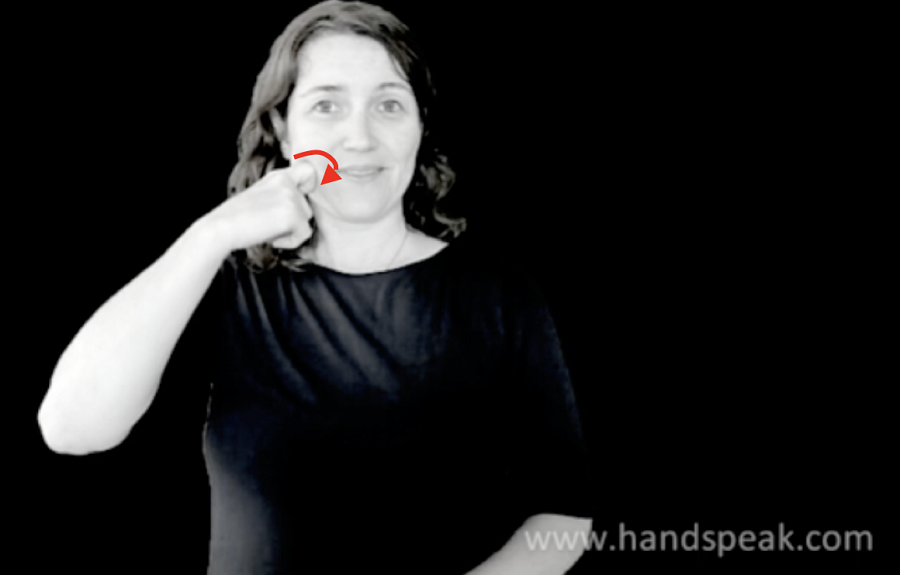
\includegraphics{../images/asl_apple.png}
\caption{APPLE}
\end{figure}
\begin{figure}[H]
\includegraphics{../images/asl_onion.png}
\caption{ONION}
\end{figure}

~\\
INSTRUCTOR NOTES: shows contrast, because handshape and movement are the same


\vfill
Excellent (3) ~~~ Good (2.2) ~~~ Fair (1.7) ~~~ Poor (0)
\newpage

\begin{center}
\textbf{{\color{red}{\HUGE END OF EXAM}}}\\

\end{center}
\newpage

\begin{center}
\textbf{{\color{blue}{\HUGE START OF EXAM\\}}}

\textbf{{\color{blue}{\HUGE Student ID: 20054\\}}}

\textbf{{\color{blue}{\HUGE \\}}}

\end{center}
\newpage

{\large Question 1}\\

Topic: Transcription\\
Source: Week 2 Handout, Part II, Question 11\\

How would this word be transcribed?\\ (Kathleen will then ask a follow-up question about your transcription.)\\

<frog>


~\\
INSTRUCTOR NOTES: [fɹɑɡ]


\vfill
Excellent (3) ~~~ Good (2.2) ~~~ Fair (1.7) ~~~ Poor (0)
\newpage

{\large Question 2}\\

Topic: Articulatory Phonetics\\
Source: Week 3 Discussion\\

Describe what the tongue would do / where it would move during each of the vowels in this word.\\

<puny>


~\\
INSTRUCTOR NOTES: 


\vfill
Excellent (3) ~~~ Good (2.2) ~~~ Fair (1.7) ~~~ Poor (0)
\newpage

{\large Question 3}\\

Topic: Phonological Features\\
Source: Quiz 3, Question 12\\

Explain how you figure out which feature is involved in the process of umlaut shown below.\\

\begin{figure}[H]
\includegraphics{../images/dutch.png}
\end{figure}

~\\
INSTRUCTOR NOTES: we look to see which vowels are affected, and compare them to see which feature is DIFFERENT (not e.g. what features they share); so since the vowels in the singular and plural are identical except that the singular forms are back and the plural are front, it's the feature [back] that is relevant / changing / involved (not e.g. the feature [round] just because all of the vowels are round)


\vfill
Excellent (3) ~~~ Good (2.2) ~~~ Fair (1.7) ~~~ Poor (0)
\newpage

{\large Question 4}\\

Topic: Skewed Distributions\\
Source: Week 5 Handout, Question 3\\

What evidence is there that there is a pattern in these data, assuming that these are the only CV and VC sequences that occur in some language?\\

{[sa]}, {[ʃi]}, {[za]}, {[ʒi]}, {[as]}, {[iʃ]}, {[az]}, {[iʒ]}


~\\
INSTRUCTOR NOTES: (the palatal sounds occur with the high vowel, while the alveolar sounds occur with the low vowel)


\vfill
Excellent (3) ~~~ Good (2.2) ~~~ Fair (1.7) ~~~ Poor (0)
\newpage

{\large Question 5}\\

Topic: Phonological Relationships and Analysis\\
Source: Week 6 Handout, Question 11\\

What do the two signs below tell you about the phonological status of \underline{handshape} in ASL, and why?\\

\begin{figure}[H]
\includegraphics{../images/asl_apple.png}
\caption{APPLE}
\end{figure}
\begin{figure}[H]
\includegraphics{../images/asl_now.png}
\caption{NOW}
\end{figure}

~\\
INSTRUCTOR NOTES: nothing, because handshape and location and movement are all also different


\vfill
Excellent (3) ~~~ Good (2.2) ~~~ Fair (1.7) ~~~ Poor (0)
\newpage

\begin{center}
\textbf{{\color{red}{\HUGE END OF EXAM}}}\\

\end{center}
\newpage

\begin{center}
\textbf{{\color{blue}{\HUGE START OF EXAM\\}}}

\textbf{{\color{blue}{\HUGE Student ID: 22413\\}}}

\textbf{{\color{blue}{\HUGE \\}}}

\end{center}
\newpage

{\large Question 1}\\

Topic: Transcription\\
Source: Week 2 Handout, Part II, Question 11\\

How would this word be transcribed?\\ (Kathleen will then ask a follow-up question about your transcription.)\\

<segment>


~\\
INSTRUCTOR NOTES: [sɛɡmɛnt]


\vfill
Excellent (3) ~~~ Good (2.2) ~~~ Fair (1.7) ~~~ Poor (0)
\newpage

{\large Question 2}\\

Topic: Articulatory Phonetics\\
Source: Week 3 Handout, Question 7\\

Is the symbol given a reasonable way to transcribe any of the sounds described below? If so, which one? If not, why not? Explain your answer.\\

{[v]}

\begin{itemize} \item voiceless palatal affricate \item voiced velar nasal \item voiceless glottal fricative \item voiced labiodental fricative \item voiced interdental fricative \item voiced palatal fricative \end{itemize}


~\\
INSTRUCTOR NOTES: yes (voiced labiodental fricative)


\vfill
Excellent (3) ~~~ Good (2.2) ~~~ Fair (1.7) ~~~ Poor (0)
\newpage

{\large Question 3}\\

Topic: Phonological Features\\
Source: Week 4 Discussion\\

Explain what the given feature’s value is for this class of sounds, and why.\\

{[approximant]}

nasals


~\\
INSTRUCTOR NOTES: [-], because air can't escape through the mouth ([+approx] sounds have a narrowing in the vocal tract, but air escapes without friction)


\vfill
Excellent (3) ~~~ Good (2.2) ~~~ Fair (1.7) ~~~ Poor (0)
\newpage

{\large Question 4}\\

Topic: Skewed Distributions\\
Source: Week 5 Handout, Question 5\\

Explain why looking for patterns with consonants and vowels is a more reasonable approach to pattern finding in this dataset than looking for patterns with respect to all of the individual sounds in Ukrainian.\\

\begin{figure}[H]
\includegraphics{../images/ukrainian.png}
\end{figure}

~\\
INSTRUCTOR NOTES: Collapsing sounds into "consonants" and "vowels" allows us to have 'sufficient data' in a way that thinking about all the individual combinations of sounds would not.


\vfill
Excellent (3) ~~~ Good (2.2) ~~~ Fair (1.7) ~~~ Poor (0)
\newpage

{\large Question 5}\\

Topic: Phonological Relationships and Analysis\\
Source: Week 6 Handout, Question 11\\

What do the two signs below tell you about the phonological status of \underline{handshape} in ASL, and why?\\

\begin{figure}[H]
\includegraphics{../images/asl_stay.png}
\caption{STAY}
\end{figure}
\begin{figure}[H]
\includegraphics{../images/asl_awkward.png}
\caption{AWKWARD}
\end{figure}

~\\
INSTRUCTOR NOTES: nothing, because both handshape and movement are different


\vfill
Excellent (3) ~~~ Good (2.2) ~~~ Fair (1.7) ~~~ Poor (0)
\newpage

\begin{center}
\textbf{{\color{red}{\HUGE END OF EXAM}}}\\

\end{center}
\newpage

\begin{center}
\textbf{{\color{blue}{\HUGE START OF EXAM\\}}}

\textbf{{\color{blue}{\HUGE Student ID: 23000\\}}}

\textbf{{\color{blue}{\HUGE \\}}}

\end{center}
\newpage

{\large Question 1}\\

Topic: Transcription\\
Source: Week 2 Handout, Part II\\

Is this a reasonable transcription of this word? Explain why.\\

<shows>: {[ʃoʊs]}


~\\
INSTRUCTOR NOTES: no, [z]


\vfill
Excellent (3) ~~~ Good (2.2) ~~~ Fair (1.7) ~~~ Poor (0)
\newpage

{\large Question 2}\\

Topic: Articulatory Phonetics\\
Source: Homework 1, Question 3(b)\\

Explain why this is or is not a complete phonetic natural class in standard North American English.\\

{[f]}, {[s]}, {[ʃ]}


~\\
INSTRUCTOR NOTES: no; voiceless fricatives include [θ], [h]


\vfill
Excellent (3) ~~~ Good (2.2) ~~~ Fair (1.7) ~~~ Poor (0)
\newpage

{\large Question 3}\\

Topic: Phonological Features\\
Source: Quiz 3, Question 3\\

Explain why this featural specification either does or does not match the given sound.\\

{[-consonantal]}, {[-sonorant]}

{[u]}


~\\
INSTRUCTOR NOTES: does not match: [u] is [-cons], but is [+son]


\vfill
Excellent (3) ~~~ Good (2.2) ~~~ Fair (1.7) ~~~ Poor (0)
\newpage

{\large Question 4}\\

Topic: Skewed Distributions\\
Source: Week 5 Handout, Question 1\\

Explain why we think that languages are not random in terms of their phonology.\\


~\\
INSTRUCTOR NOTES: 


\vfill
Excellent (3) ~~~ Good (2.2) ~~~ Fair (1.7) ~~~ Poor (0)
\newpage

{\large Question 5}\\

Topic: Phonological Relationships and Analysis\\
Source: Week 6 Handout, Question 11\\

What do the two signs below tell you about the phonological status of \underline{handshape} in ASL, and why?\\

\begin{figure}[H]
\includegraphics{../images/asl_apple.png}
\caption{APPLE}
\end{figure}
\begin{figure}[H]
\includegraphics{../images/asl_now.png}
\caption{NOW}
\end{figure}

~\\
INSTRUCTOR NOTES: nothing, because handshape and location and movement are all also different


\vfill
Excellent (3) ~~~ Good (2.2) ~~~ Fair (1.7) ~~~ Poor (0)
\newpage

\begin{center}
\textbf{{\color{red}{\HUGE END OF EXAM}}}\\

\end{center}
\newpage

\begin{center}
\textbf{{\color{blue}{\HUGE START OF EXAM\\}}}

\textbf{{\color{blue}{\HUGE Student ID: 23071\\}}}

\textbf{{\color{blue}{\HUGE \\}}}

\end{center}
\newpage

{\large Question 1}\\

Topic: Transcription\\
Source: Week 2 Handout, Part II, Question 11\\

How would this word be transcribed?\\ (Kathleen will then ask a follow-up question about your transcription.)\\

<finger>


~\\
INSTRUCTOR NOTES: [fɪŋɡɹ̩]


\vfill
Excellent (3) ~~~ Good (2.2) ~~~ Fair (1.7) ~~~ Poor (0)
\newpage

{\large Question 2}\\

Topic: Articulatory Phonetics\\
Source: Week 2 Handout, Part I, Question 12\\

Explain in what sense the difference between the sounds in the words <but> and <cut> is SIMILAR to and also DIFFERENT from the difference between the sounds in the words <bit> and <kit>.\\


~\\
INSTRUCTOR NOTES: 


\vfill
Excellent (3) ~~~ Good (2.2) ~~~ Fair (1.7) ~~~ Poor (0)
\newpage

{\large Question 3}\\

Topic: Phonological Features\\
Source: Week 4 Discussion\\

Explain what the given feature’s value is for this class of sounds, and why.\\

{[continuant]}

glottals


~\\
INSTRUCTOR NOTES: 0, because there is no constriction in the vocal tract for manner features to apply


\vfill
Excellent (3) ~~~ Good (2.2) ~~~ Fair (1.7) ~~~ Poor (0)
\newpage

{\large Question 4}\\

Topic: Skewed Distributions\\
Source: Week 5 Handout, Question 7\\

Explain how you would go about looking for co-occurrence restrictions in bi-syllabic signs in ASL. (Refer to the data that follows.)\\

\begin{figure}[H]
\includegraphics{../images/ASL_movement.png}
\end{figure}

~\\
INSTRUCTOR NOTES: You would start by coming up with all the possible combinations expected (i.e., 4x4 = 16). Then you'd compare that to some database of signs in ASL and see which combinations are actually attested or unattested.


\vfill
Excellent (3) ~~~ Good (2.2) ~~~ Fair (1.7) ~~~ Poor (0)
\newpage

{\large Question 5}\\

Topic: Phonological Relationships and Analysis\\
Source: Week 7 Handout, Question 9\\

What is the basic analysis of vowel length in this dataset, and what are the key pieces of evidence?\\

\begin{figure}[H]
\includegraphics{../images/malayalam.png}
\end{figure}

~\\
INSTRUCTOR NOTES: Short and long vowels appear to be contrastive (phonemic) in Malayalam, as evidenced by minimal pairs that differ only in terms of their vowel length, such as [koʈːa] ‘basket’ vs. [koːʈːa] ‘castle’ or [keʈːu] ‘burnt out’ vs. [keːʈːu] ‘heard.’


\vfill
Excellent (3) ~~~ Good (2.2) ~~~ Fair (1.7) ~~~ Poor (0)
\newpage

\begin{center}
\textbf{{\color{red}{\HUGE END OF EXAM}}}\\

\end{center}
\newpage

\begin{center}
\textbf{{\color{blue}{\HUGE START OF EXAM\\}}}

\textbf{{\color{blue}{\HUGE Student ID: 23100\\}}}

\textbf{{\color{blue}{\HUGE \\}}}

\end{center}
\newpage

{\large Question 1}\\

Topic: Transcription\\
Source: Week 2 Handout, Part II\\

Is this a reasonable transcription of this word? Explain why.\\

<mine>: {[mɑɪn]}


~\\
INSTRUCTOR NOTES: yes


\vfill
Excellent (3) ~~~ Good (2.2) ~~~ Fair (1.7) ~~~ Poor (0)
\newpage

{\large Question 2}\\

Topic: Articulatory Phonetics\\
Source: Week 3 Discussion\\

Assuming a Standard North American English inventory, does this vowel need to have tenseness specified if you're giving a prose description? Why or why not?\\

{[ɛ]}


~\\
INSTRUCTOR NOTES: yes


\vfill
Excellent (3) ~~~ Good (2.2) ~~~ Fair (1.7) ~~~ Poor (0)
\newpage

{\large Question 3}\\

Topic: Phonological Features\\
Source: Homework 2, Question 1\\

Explain which sound should be removed to make this a natural class (assuming SNAE, except that there are no diphthongs, no [ə] or [ʌ], no syllabic consonants, and no [w̥]), and what the minimum set of features would be to describe the resulting natural class.\\

{[b]}, {[d]}, {[z]}, {[ɾ]}, {[n]}, {[l]}, {[ɹ]}


~\\
INSTRUCTOR NOTES: [b] should be removed, so that we have the natural class of voiced alveolars; this could be minimally represented with [+voice, -distributed]


\vfill
Excellent (3) ~~~ Good (2.2) ~~~ Fair (1.7) ~~~ Poor (0)
\newpage

{\large Question 4}\\

Topic: Skewed Distributions\\
Source: Week 5 Handout, Question 5\\

Explain why it is possible to predict which of [s] or [ʃʲ] will occur in a new environment in Ukrainian, but not possible to predict which of [s] or [ʃ] will occur in a new environment.\\

\begin{figure}[H]
\includegraphics{../images/ukrainian.png}
\end{figure}

~\\
INSTRUCTOR NOTES: [s] and [S] have the same pattern of co-occurrence restrictions, so they occur in the same environments, and you cannot predict which one will occur where. [s] and [Sj] on the other hand have 'opposite' patterns, so you can always predict which will occur based on the vowel.


\vfill
Excellent (3) ~~~ Good (2.2) ~~~ Fair (1.7) ~~~ Poor (0)
\newpage

{\large Question 5}\\

Topic: Phonological Relationships and Analysis\\
Source: Week 6 Handout, Question 11\\

What do the two signs below tell you about the phonological status of \underline{handshape} in ASL, and why?\\

\begin{figure}[H]
\includegraphics{../images/asl_apple.png}
\caption{APPLE}
\end{figure}
\begin{figure}[H]
\includegraphics{../images/asl_candy.png}
\caption{CANDY}
\end{figure}

~\\
INSTRUCTOR NOTES: shows contrast because movement and location are same


\vfill
Excellent (3) ~~~ Good (2.2) ~~~ Fair (1.7) ~~~ Poor (0)
\newpage

\begin{center}
\textbf{{\color{red}{\HUGE END OF EXAM}}}\\

\end{center}
\newpage

\begin{center}
\textbf{{\color{blue}{\HUGE START OF EXAM\\}}}

\textbf{{\color{blue}{\HUGE Student ID: 23286\\}}}

\textbf{{\color{blue}{\HUGE \\}}}

\end{center}
\newpage

{\large Question 1}\\

Topic: Transcription\\
Source: Week 2 Handout, Part II, Question 11\\

How would this word be transcribed?\\ (Kathleen will then ask a follow-up question about your transcription.)\\

<finger>


~\\
INSTRUCTOR NOTES: [fɪŋɡɹ̩]


\vfill
Excellent (3) ~~~ Good (2.2) ~~~ Fair (1.7) ~~~ Poor (0)
\newpage

{\large Question 2}\\

Topic: Articulatory Phonetics\\
Source: Week 3 Handout, Question 3\\

Explain why the additional vowel below either does or does not belong in the phonetic natural class defined by the original set of SNAE vowels.\\

Original set: {[ɛ]}, {[ɪ]}, {[ʊ]}, {[ɔ]}

Addition: {[ɑ]}


~\\
INSTRUCTOR NOTES: new vowel is a low vowel; should recognize that there's more than one decision about low vowels and tenseness; default is to say it doesn't belong in the class because tenseness is irrelevant


\vfill
Excellent (3) ~~~ Good (2.2) ~~~ Fair (1.7) ~~~ Poor (0)
\newpage

{\large Question 3}\\

Topic: Phonological Features\\
Source: Week 4 Discussion\\

Explain what the given feature’s value is for this class of sounds, and why.\\

{[LABIAL]}

interdentals


~\\
INSTRUCTOR NOTES: 0, because interdentals aren't [LABIAL], but [LABIAL] is monovalent, so they're not [-labial]


\vfill
Excellent (3) ~~~ Good (2.2) ~~~ Fair (1.7) ~~~ Poor (0)
\newpage

{\large Question 4}\\

Topic: Skewed Distributions\\
Source: Week 5 Handout, Question 5\\

Explain why it is possible to predict which of [s] or [ʃʲ] will occur in a new environment in Ukrainian, but not possible to predict which of [s] or [ʃ] will occur in a new environment.\\

\begin{figure}[H]
\includegraphics{../images/ukrainian.png}
\end{figure}

~\\
INSTRUCTOR NOTES: [s] and [S] have the same pattern of co-occurrence restrictions, so they occur in the same environments, and you cannot predict which one will occur where. [s] and [Sj] on the other hand have 'opposite' patterns, so you can always predict which will occur based on the vowel.


\vfill
Excellent (3) ~~~ Good (2.2) ~~~ Fair (1.7) ~~~ Poor (0)
\newpage

{\large Question 5}\\

Topic: Phonological Relationships and Analysis\\
Source: Week 7 Handout, Question 12\\

What is the basic analysis of oral and nasal vowels in this dataset, and what are the key pieces of evidence?\\

\begin{figure}[H]
\includegraphics{../images/english12.png}
\end{figure}

~\\
INSTRUCTOR NOTES: The pairs of sounds [i] and [ĩ], and [u] and [ũ], are each allophonic and therefore allophones of the same phoneme in English (though the two pairs represent two contrastive phonemes in English). The sounds [i] and [ĩ] are in complementary distribution in English, with [ĩ] occurring before the sounds [m] and [n], (e.g., [ɡlĩm] ‘gleam’ and [klĩn] ‘clean’) and [i] occurring elsewhere (e.g., [lip] ‘leap’). Similarly, the sounds [u] and [ũ] are also in complementary distribution, with exactly the same conditioning environments: [ũ] occurs before [m] and [n] (e.g., [dũm] ‘doom’ and [dũn] ‘dune’), and [u] occurs elsewhere (e.g. [but] ‘boot’). Thus, within each pair, we treat the vowels as allophonic. 


\vfill
Excellent (3) ~~~ Good (2.2) ~~~ Fair (1.7) ~~~ Poor (0)
\newpage

\begin{center}
\textbf{{\color{red}{\HUGE END OF EXAM}}}\\

\end{center}
\newpage

\begin{center}
\textbf{{\color{blue}{\HUGE START OF EXAM\\}}}

\textbf{{\color{blue}{\HUGE Student ID: 24476\\}}}

\textbf{{\color{blue}{\HUGE \\}}}

\end{center}
\newpage

{\large Question 1}\\

Topic: Transcription\\
Source: Week 2 Handout, Part II, Question 11\\

How would this word be transcribed?\\ (Kathleen will then ask a follow-up question about your transcription.)\\

<wealth>


~\\
INSTRUCTOR NOTES: [wɛlθ]


\vfill
Excellent (3) ~~~ Good (2.2) ~~~ Fair (1.7) ~~~ Poor (0)
\newpage

{\large Question 2}\\

Topic: Articulatory Phonetics\\
Source: Week 3 Handout, Question 7\\

Is the symbol given a reasonable way to transcribe any of the sounds described below? If so, which one? If not, why not? Explain your answer.\\

{[ʒ]}

\begin{itemize} \item voiceless palatal affricate \item voiced velar nasal \item voiceless glottal fricative \item voiced labiodental fricative \item voiced interdental fricative \item voiced palatal fricative \end{itemize}


~\\
INSTRUCTOR NOTES: yes (voiced palatal fricative)


\vfill
Excellent (3) ~~~ Good (2.2) ~~~ Fair (1.7) ~~~ Poor (0)
\newpage

{\large Question 3}\\

Topic: Phonological Features\\
Source: Homework 2, Question 1\\

Explain which sound should be removed to make this a natural class (assuming SNAE, except that there are no diphthongs, no [ə] or [ʌ], no syllabic consonants, and no [w̥]), and what the minimum set of features would be to describe the resulting natural class.\\

{[b]}, {[d]}, {[z]}, {[ɾ]}, {[n]}, {[l]}, {[ɹ]}


~\\
INSTRUCTOR NOTES: [b] should be removed, so that we have the natural class of voiced alveolars; this could be minimally represented with [+voice, -distributed]


\vfill
Excellent (3) ~~~ Good (2.2) ~~~ Fair (1.7) ~~~ Poor (0)
\newpage

{\large Question 4}\\

Topic: Skewed Distributions\\
Source: Week 5 Handout, Question 7\\

Explain how you would go about looking for co-occurrence restrictions in bi-syllabic signs in ASL. (Refer to the data that follows.)\\

\begin{figure}[H]
\includegraphics{../images/ASL_movement.png}
\end{figure}

~\\
INSTRUCTOR NOTES: You would start by coming up with all the possible combinations expected (i.e., 4x4 = 16). Then you'd compare that to some database of signs in ASL and see which combinations are actually attested or unattested.


\vfill
Excellent (3) ~~~ Good (2.2) ~~~ Fair (1.7) ~~~ Poor (0)
\newpage

{\large Question 5}\\

Topic: Phonological Relationships and Analysis\\
Source: Week 7 Handout, Question 9\\

What is the basic analysis of vowel length in this dataset, and what are the key pieces of evidence?\\

\begin{figure}[H]
\includegraphics{../images/malayalam.png}
\end{figure}

~\\
INSTRUCTOR NOTES: Short and long vowels appear to be contrastive (phonemic) in Malayalam, as evidenced by minimal pairs that differ only in terms of their vowel length, such as [koʈːa] ‘basket’ vs. [koːʈːa] ‘castle’ or [keʈːu] ‘burnt out’ vs. [keːʈːu] ‘heard.’


\vfill
Excellent (3) ~~~ Good (2.2) ~~~ Fair (1.7) ~~~ Poor (0)
\newpage

\begin{center}
\textbf{{\color{red}{\HUGE END OF EXAM}}}\\

\end{center}
\newpage

\begin{center}
\textbf{{\color{blue}{\HUGE START OF EXAM\\}}}

\textbf{{\color{blue}{\HUGE Student ID: 27121\\}}}

\textbf{{\color{blue}{\HUGE \\}}}

\end{center}
\newpage

{\large Question 1}\\

Topic: Transcription\\
Source: Week 2 Handout, Part II, Question 11\\

How would this word be transcribed?\\ (Kathleen will then ask a follow-up question about your transcription.)\\

<segment>


~\\
INSTRUCTOR NOTES: [sɛɡmɛnt]


\vfill
Excellent (3) ~~~ Good (2.2) ~~~ Fair (1.7) ~~~ Poor (0)
\newpage

{\large Question 2}\\

Topic: Articulatory Phonetics\\
Source: Week 3 Discussion\\

Describe what the tongue would do / where it would move during each of the vowels in this word.\\

<follow>


~\\
INSTRUCTOR NOTES: 


\vfill
Excellent (3) ~~~ Good (2.2) ~~~ Fair (1.7) ~~~ Poor (0)
\newpage

{\large Question 3}\\

Topic: Phonological Features\\
Source: Week 4 Discussion\\

Explain what the given feature’s value is for this class of sounds, and why.\\

{[consonantal]}

glides


~\\
INSTRUCTOR NOTES: [-], because the constriction isn't as narrow as it would be for a fricative


\vfill
Excellent (3) ~~~ Good (2.2) ~~~ Fair (1.7) ~~~ Poor (0)
\newpage

{\large Question 4}\\

Topic: Skewed Distributions\\
Source: Week 5 Handout, Question 6\\

If I gave you a new word in Malto, [di\_\_u], would it be possible to predict whether it's [d] or [ɖ] that goes in the blank? Explain why or why not.\\

\begin{figure}[H]
\includegraphics{../images/malto.png}
\end{figure}

~\\
INSTRUCTOR NOTES: Yes, it's possible; in Malto, if there are two stops in a word, they must either both be dental or both retroflex. Since the first sound is dental, the second must also be dental (though to be fair, you couldn't actually predict that it's [d] and not [t], but the question restricts it to only the voiced options).


\vfill
Excellent (3) ~~~ Good (2.2) ~~~ Fair (1.7) ~~~ Poor (0)
\newpage

{\large Question 5}\\

Topic: Phonological Relationships and Analysis\\
Source: Week 6 Handout, Question 11\\

What do the two signs below tell you about the phonological status of \underline{handshape} in ASL, and why?\\

\begin{figure}[H]
\includegraphics{../images/asl_apple.png}
\caption{APPLE}
\end{figure}
\begin{figure}[H]
\includegraphics{../images/asl_onion.png}
\caption{ONION}
\end{figure}

~\\
INSTRUCTOR NOTES: shows contrast, because handshape and movement are the same


\vfill
Excellent (3) ~~~ Good (2.2) ~~~ Fair (1.7) ~~~ Poor (0)
\newpage

\begin{center}
\textbf{{\color{red}{\HUGE END OF EXAM}}}\\

\end{center}
\newpage

\begin{center}
\textbf{{\color{blue}{\HUGE START OF EXAM\\}}}

\textbf{{\color{blue}{\HUGE Student ID: 27762\\}}}

\textbf{{\color{blue}{\HUGE \\}}}

\end{center}
\newpage

{\large Question 1}\\

Topic: Transcription\\
Source: Week 2 Handout, Part II, Question 11\\

How would this word be transcribed?\\ (Kathleen will then ask a follow-up question about your transcription.)\\

<cough>


~\\
INSTRUCTOR NOTES: [kɑf]


\vfill
Excellent (3) ~~~ Good (2.2) ~~~ Fair (1.7) ~~~ Poor (0)
\newpage

{\large Question 2}\\

Topic: Articulatory Phonetics\\
Source: Week 3 Handout, Question 7\\

Is the symbol given a reasonable way to transcribe any of the sounds described below? If so, which one? If not, why not? Explain your answer.\\

{[ʒ]}

\begin{itemize} \item voiceless palatal affricate \item voiced velar nasal \item voiceless glottal fricative \item voiced labiodental fricative \item voiced interdental fricative \item voiced palatal fricative \end{itemize}


~\\
INSTRUCTOR NOTES: yes (voiced palatal fricative)


\vfill
Excellent (3) ~~~ Good (2.2) ~~~ Fair (1.7) ~~~ Poor (0)
\newpage

{\large Question 3}\\

Topic: Phonological Features\\
Source: Homework 2, Question 1\\

Explain which sound should be removed to make this a natural class (assuming SNAE, except that there are no diphthongs, no [ə] or [ʌ], no syllabic consonants, and no [w̥]), and what the minimum set of features would be to describe the resulting natural class.\\

{[i]}, {[ɪ]}, {[e]}, {[ɛ]}, {[æ]}, {[ɑ]}, {[ɔ]}, {[o]}, {[ʊ]}, {[u]}, {[ʒ]}, {[k]}, {[ɡ]}, {[ŋ]}, {[w]}


~\\
INSTRUCTOR NOTES: [ʒ] should be removed, so that we have the natural class of dorsal segments; this could be minimally represented with [DORSAL]


\vfill
Excellent (3) ~~~ Good (2.2) ~~~ Fair (1.7) ~~~ Poor (0)
\newpage

{\large Question 4}\\

Topic: Skewed Distributions\\
Source: Week 5 Handout, Question 5\\

Explain why looking for patterns with consonants and vowels is a more reasonable approach to pattern finding in this dataset than looking for patterns with respect to all of the individual sounds in Ukrainian.\\

\begin{figure}[H]
\includegraphics{../images/ukrainian.png}
\end{figure}

~\\
INSTRUCTOR NOTES: Collapsing sounds into "consonants" and "vowels" allows us to have 'sufficient data' in a way that thinking about all the individual combinations of sounds would not.


\vfill
Excellent (3) ~~~ Good (2.2) ~~~ Fair (1.7) ~~~ Poor (0)
\newpage

{\large Question 5}\\

Topic: Phonological Relationships and Analysis\\
Source: Week 7 Handout, Question 12\\

What is the basic analysis of oral and nasal vowels in this dataset, and what are the key pieces of evidence?\\

\begin{figure}[H]
\includegraphics{../images/english12.png}
\end{figure}

~\\
INSTRUCTOR NOTES: The pairs of sounds [i] and [ĩ], and [u] and [ũ], are each allophonic and therefore allophones of the same phoneme in English (though the two pairs represent two contrastive phonemes in English). The sounds [i] and [ĩ] are in complementary distribution in English, with [ĩ] occurring before the sounds [m] and [n], (e.g., [ɡlĩm] ‘gleam’ and [klĩn] ‘clean’) and [i] occurring elsewhere (e.g., [lip] ‘leap’). Similarly, the sounds [u] and [ũ] are also in complementary distribution, with exactly the same conditioning environments: [ũ] occurs before [m] and [n] (e.g., [dũm] ‘doom’ and [dũn] ‘dune’), and [u] occurs elsewhere (e.g. [but] ‘boot’). Thus, within each pair, we treat the vowels as allophonic. 


\vfill
Excellent (3) ~~~ Good (2.2) ~~~ Fair (1.7) ~~~ Poor (0)
\newpage

\begin{center}
\textbf{{\color{red}{\HUGE END OF EXAM}}}\\

\end{center}
\newpage

\begin{center}
\textbf{{\color{blue}{\HUGE START OF EXAM\\}}}

\textbf{{\color{blue}{\HUGE Student ID: 28926\\}}}

\textbf{{\color{blue}{\HUGE \\}}}

\end{center}
\newpage

{\large Question 1}\\

Topic: Transcription\\
Source: Week 2 Handout, Part II, Question 11\\

How would this word be transcribed?\\ (Kathleen will then ask a follow-up question about your transcription.)\\

<goat>


~\\
INSTRUCTOR NOTES: [ɡoʊt]


\vfill
Excellent (3) ~~~ Good (2.2) ~~~ Fair (1.7) ~~~ Poor (0)
\newpage

{\large Question 2}\\

Topic: Articulatory Phonetics\\
Source: Week 3 Discussion\\

Assuming a Standard North American English inventory, does this vowel need to have tenseness specified if you're giving a prose description? Why or why not?\\

{[u]}


~\\
INSTRUCTOR NOTES: yes


\vfill
Excellent (3) ~~~ Good (2.2) ~~~ Fair (1.7) ~~~ Poor (0)
\newpage

{\large Question 3}\\

Topic: Phonological Features\\
Source: Week 4 Discussion\\

Explain why phonological features are used instead of phonetic characteristics in analyzing datasets.\\


~\\
INSTRUCTOR NOTES: Phonological features help to capture phonological patterns, i.e., they group sounds together based on whether they do things like triggering a change or undergoing a change. Phonological features are sometimes language-specific. Phonetic characteristics are simply descriptions of the physical properties of the sounds; they are language-universal and independent of the patterns (though it turns out that many phonological patterns are based on phonetic characteristic groupings).


\vfill
Excellent (3) ~~~ Good (2.2) ~~~ Fair (1.7) ~~~ Poor (0)
\newpage

{\large Question 4}\\

Topic: Skewed Distributions\\
Source: Week 5 Handout, Question 2\\

Explain why there should only be 8 sequences listed in the answer, even though multiplying 4 x 4 would give you 16 possible sequences.\\

\begin{figure}[H]
\includegraphics{../images/skew2.png}
\end{figure}

~\\
INSTRUCTOR NOTES: The instructions say that you're only supposed to consider CV and VC sequences. 


\vfill
Excellent (3) ~~~ Good (2.2) ~~~ Fair (1.7) ~~~ Poor (0)
\newpage

{\large Question 5}\\

Topic: Phonological Relationships and Analysis\\
Source: Week 7 Handout, Question 9\\

What is the basic analysis of vowel length in this dataset, and what are the key pieces of evidence?\\

\begin{figure}[H]
\includegraphics{../images/malayalam.png}
\end{figure}

~\\
INSTRUCTOR NOTES: Short and long vowels appear to be contrastive (phonemic) in Malayalam, as evidenced by minimal pairs that differ only in terms of their vowel length, such as [koʈːa] ‘basket’ vs. [koːʈːa] ‘castle’ or [keʈːu] ‘burnt out’ vs. [keːʈːu] ‘heard.’


\vfill
Excellent (3) ~~~ Good (2.2) ~~~ Fair (1.7) ~~~ Poor (0)
\newpage

\begin{center}
\textbf{{\color{red}{\HUGE END OF EXAM}}}\\

\end{center}
\newpage

\begin{center}
\textbf{{\color{blue}{\HUGE START OF EXAM\\}}}

\textbf{{\color{blue}{\HUGE Student ID: 29164\\}}}

\textbf{{\color{blue}{\HUGE \\}}}

\end{center}
\newpage

{\large Question 1}\\

Topic: Transcription\\
Source: Week 2 Handout, Part II\\

Is this a reasonable transcription of this word? Explain why.\\

<paid>: {[peid]}


~\\
INSTRUCTOR NOTES: okay, but [eɪ]


\vfill
Excellent (3) ~~~ Good (2.2) ~~~ Fair (1.7) ~~~ Poor (0)
\newpage

{\large Question 2}\\

Topic: Articulatory Phonetics\\
Source: Week 3 Handout, Question 7\\

Is the symbol given a reasonable way to transcribe any of the sounds described below? If so, which one? If not, why not? Explain your answer.\\

{[ʒ]}

\begin{itemize} \item voiceless palatal affricate \item voiced velar nasal \item voiceless glottal fricative \item voiced labiodental fricative \item voiced interdental fricative \item voiced palatal fricative \end{itemize}


~\\
INSTRUCTOR NOTES: yes (voiced palatal fricative)


\vfill
Excellent (3) ~~~ Good (2.2) ~~~ Fair (1.7) ~~~ Poor (0)
\newpage

{\large Question 3}\\

Topic: Phonological Features\\
Source: Homework 2, Question 1\\

Explain which sound should be removed to make this a natural class (assuming SNAE, except that there are no diphthongs, no [ə] or [ʌ], no syllabic consonants, and no [w̥]), and what the minimum set of features would be to describe the resulting natural class.\\

{[i]}, {[ɪ]}, {[ɛ]}, {[u]}, {[ʊ]}


~\\
INSTRUCTOR NOTES: [ɛ] should be removed, so that we have the natural class of high vowels; this could be minimally represented with [+syll, +high]


\vfill
Excellent (3) ~~~ Good (2.2) ~~~ Fair (1.7) ~~~ Poor (0)
\newpage

{\large Question 4}\\

Topic: Skewed Distributions\\
Source: Week 5 Handout, Question 1\\

Explain why we think that languages are not random in terms of their phonology.\\


~\\
INSTRUCTOR NOTES: 


\vfill
Excellent (3) ~~~ Good (2.2) ~~~ Fair (1.7) ~~~ Poor (0)
\newpage

{\large Question 5}\\

Topic: Phonological Relationships and Analysis\\
Source: Week 6 Handout, Question 11\\

What do the two signs below tell you about the phonological status of \underline{handshape} in ASL, and why?\\

\begin{figure}[H]
\includegraphics{../images/asl_apple.png}
\caption{APPLE}
\end{figure}
\begin{figure}[H]
\includegraphics{../images/asl_candy.png}
\caption{CANDY}
\end{figure}

~\\
INSTRUCTOR NOTES: shows contrast because movement and location are same


\vfill
Excellent (3) ~~~ Good (2.2) ~~~ Fair (1.7) ~~~ Poor (0)
\newpage

\begin{center}
\textbf{{\color{red}{\HUGE END OF EXAM}}}\\

\end{center}
\newpage

\begin{center}
\textbf{{\color{blue}{\HUGE START OF EXAM\\}}}

\textbf{{\color{blue}{\HUGE Student ID: 30263\\}}}

\textbf{{\color{blue}{\HUGE \\}}}

\end{center}
\newpage

{\large Question 1}\\

Topic: Transcription\\
Source: Week 2 Handout, Part II, Question 3\\

Explain why people might legitimately disagree about how many sounds this particular word contains.\\

<rice>


~\\
INSTRUCTOR NOTES: 


\vfill
Excellent (3) ~~~ Good (2.2) ~~~ Fair (1.7) ~~~ Poor (0)
\newpage

{\large Question 2}\\

Topic: Articulatory Phonetics\\
Source: Week 3 Handout, Question 3\\

Explain why the additional vowel below either does or does not belong in the phonetic natural class defined by the original set of SNAE vowels.\\

Original set: {[ɛ]}, {[ɪ]}, {[ʊ]}, {[ɔ]}

Addition: {[ɑ]}


~\\
INSTRUCTOR NOTES: new vowel is a low vowel; should recognize that there's more than one decision about low vowels and tenseness; default is to say it doesn't belong in the class because tenseness is irrelevant


\vfill
Excellent (3) ~~~ Good (2.2) ~~~ Fair (1.7) ~~~ Poor (0)
\newpage

{\large Question 3}\\

Topic: Phonological Features\\
Source: Homework 2, Question 1\\

Explain which sound should be removed to make this a natural class (assuming SNAE, except that there are no diphthongs, no [ə] or [ʌ], no syllabic consonants, and no [w̥]), and what the minimum set of features would be to describe the resulting natural class.\\

{[b]}, {[d]}, {[z]}, {[ɾ]}, {[n]}, {[l]}, {[ɹ]}


~\\
INSTRUCTOR NOTES: [b] should be removed, so that we have the natural class of voiced alveolars; this could be minimally represented with [+voice, -distributed]


\vfill
Excellent (3) ~~~ Good (2.2) ~~~ Fair (1.7) ~~~ Poor (0)
\newpage

{\large Question 4}\\

Topic: Skewed Distributions\\
Source: Week 5 Handout, Question 1\\

Explain why we think that languages are not random in terms of their phonology.\\


~\\
INSTRUCTOR NOTES: 


\vfill
Excellent (3) ~~~ Good (2.2) ~~~ Fair (1.7) ~~~ Poor (0)
\newpage

{\large Question 5}\\

Topic: Phonological Relationships and Analysis\\
Source: Week 6 Handout, Question 11\\

What do the two signs below tell you about the phonological status of \underline{handshape} in ASL, and why?\\

\begin{figure}[H]
\includegraphics{../images/asl_apple.png}
\caption{APPLE}
\end{figure}
\begin{figure}[H]
\includegraphics{../images/asl_onion.png}
\caption{ONION}
\end{figure}

~\\
INSTRUCTOR NOTES: shows contrast, because handshape and movement are the same


\vfill
Excellent (3) ~~~ Good (2.2) ~~~ Fair (1.7) ~~~ Poor (0)
\newpage

\begin{center}
\textbf{{\color{red}{\HUGE END OF EXAM}}}\\

\end{center}
\newpage

\begin{center}
\textbf{{\color{blue}{\HUGE START OF EXAM\\}}}

\textbf{{\color{blue}{\HUGE Student ID: 30511\\}}}

\textbf{{\color{blue}{\HUGE \\}}}

\end{center}
\newpage

{\large Question 1}\\

Topic: Transcription\\
Source: Quiz 1, Question 10\\

Explain whether this word either does or does not have an [ʃ] sound in it, and why the spelling and pronunciation either do or do not align.\\

<mishandle>


~\\
INSTRUCTOR NOTES: 


\vfill
Excellent (3) ~~~ Good (2.2) ~~~ Fair (1.7) ~~~ Poor (0)
\newpage

{\large Question 2}\\

Topic: Articulatory Phonetics\\
Source: Week 3 Handout, Question 13\\

Explain why this image does or does not match the description.\\

\begin{itemize} \item A one-handed sign. \item Location: At the signer’s nose. \item Handshape: Starts with index finger extended; finger folds down into a “hook” shape during the sign; then straightens and repeats the folding. \item Movement: No movement other than the change in handshape. \end{itemize}

\begin{figure}[H]
\includegraphics{../images/taiwansign_wrong.png}
\caption{WRONG}
\end{figure}

~\\
INSTRUCTOR NOTES: no; handshape is wrong


\vfill
Excellent (3) ~~~ Good (2.2) ~~~ Fair (1.7) ~~~ Poor (0)
\newpage

{\large Question 3}\\

Topic: Phonological Features\\
Source: Quiz 3, Question 12\\

Explain how you figure out which feature is involved in the process of umlaut shown below.\\

\begin{figure}[H]
\includegraphics{../images/dutch.png}
\end{figure}

~\\
INSTRUCTOR NOTES: we look to see which vowels are affected, and compare them to see which feature is DIFFERENT (not e.g. what features they share); so since the vowels in the singular and plural are identical except that the singular forms are back and the plural are front, it's the feature [back] that is relevant / changing / involved (not e.g. the feature [round] just because all of the vowels are round)


\vfill
Excellent (3) ~~~ Good (2.2) ~~~ Fair (1.7) ~~~ Poor (0)
\newpage

{\large Question 4}\\

Topic: Skewed Distributions\\
Source: Quiz 4, Question 2\\

L$_X$ (Language X) has three vowels, [i], [a], and [u]. L$_X$ has tri-syllabic roots. If L$_X$ does not allow non-identical high vowels to co-occur, which one of the following tri-syllabic vocalic sequences do you predict to be unattested in L$_X$? Explain why.\\

\begin{itemize} \item {[u...i...a]} \item {[a...i...a]} \item {[u...u...a]} \item {[a...i...i]} \end{itemize}


~\\
INSTRUCTOR NOTES: [u...i...a]


\vfill
Excellent (3) ~~~ Good (2.2) ~~~ Fair (1.7) ~~~ Poor (0)
\newpage

{\large Question 5}\\

Topic: Phonological Relationships and Analysis\\
Source: Week 7 Handout, Question 12\\

What is the basic analysis of oral and nasal vowels in this dataset, and what are the key pieces of evidence?\\

\begin{figure}[H]
\includegraphics{../images/english12.png}
\end{figure}

~\\
INSTRUCTOR NOTES: The pairs of sounds [i] and [ĩ], and [u] and [ũ], are each allophonic and therefore allophones of the same phoneme in English (though the two pairs represent two contrastive phonemes in English). The sounds [i] and [ĩ] are in complementary distribution in English, with [ĩ] occurring before the sounds [m] and [n], (e.g., [ɡlĩm] ‘gleam’ and [klĩn] ‘clean’) and [i] occurring elsewhere (e.g., [lip] ‘leap’). Similarly, the sounds [u] and [ũ] are also in complementary distribution, with exactly the same conditioning environments: [ũ] occurs before [m] and [n] (e.g., [dũm] ‘doom’ and [dũn] ‘dune’), and [u] occurs elsewhere (e.g. [but] ‘boot’). Thus, within each pair, we treat the vowels as allophonic. 


\vfill
Excellent (3) ~~~ Good (2.2) ~~~ Fair (1.7) ~~~ Poor (0)
\newpage

\begin{center}
\textbf{{\color{red}{\HUGE END OF EXAM}}}\\

\end{center}
\newpage

\begin{center}
\textbf{{\color{blue}{\HUGE START OF EXAM\\}}}

\textbf{{\color{blue}{\HUGE Student ID: 30794\\}}}

\textbf{{\color{blue}{\HUGE \\}}}

\end{center}
\newpage

{\large Question 1}\\

Topic: Transcription\\
Source: Week 2 Handout, Part II, Question 2\\

Explain why people might legitimately disagree about how many sounds this particular word contains.\\

<those>


~\\
INSTRUCTOR NOTES: 


\vfill
Excellent (3) ~~~ Good (2.2) ~~~ Fair (1.7) ~~~ Poor (0)
\newpage

{\large Question 2}\\

Topic: Articulatory Phonetics\\
Source: Quiz 2, Question 7\\

Why might more than one of the descriptions given truthfully apply to the sound represented by the underlined letter, and why is one of them actually better than the other?\\

<a\underline{w}ay>

\begin{itemize} \item prevocalic obstruent \item prevocalic sonorant \item postvocalic obstruent \item postvocalic sonorant \item intervocalic obstruent \item intervocalic sonorant \end{itemize}


~\\
INSTRUCTOR NOTES: prevocalic and *intervocalic* sonorant


\vfill
Excellent (3) ~~~ Good (2.2) ~~~ Fair (1.7) ~~~ Poor (0)
\newpage

{\large Question 3}\\

Topic: Phonological Features\\
Source: Week 4 Discussion\\

Explain why phonological features are used instead of phonetic characteristics in analyzing datasets.\\


~\\
INSTRUCTOR NOTES: Phonological features help to capture phonological patterns, i.e., they group sounds together based on whether they do things like triggering a change or undergoing a change. Phonological features are sometimes language-specific. Phonetic characteristics are simply descriptions of the physical properties of the sounds; they are language-universal and independent of the patterns (though it turns out that many phonological patterns are based on phonetic characteristic groupings).


\vfill
Excellent (3) ~~~ Good (2.2) ~~~ Fair (1.7) ~~~ Poor (0)
\newpage

{\large Question 4}\\

Topic: Skewed Distributions\\
Source: Week 5 Handout, Question 6\\

What would be a good description of the pattern in Malto? What characteristics make that a good description?\\

\begin{figure}[H]
\includegraphics{../images/malto.png}
\end{figure}

~\\
INSTRUCTOR NOTES: It is not possible to have stops of different places of articulation co-occurring in a single word. Instead, if there are two stops, both must be dental, or both must be retroflex. For example, it’s possible to have a word with two dental stops, as in [tot] ‘to hurry’ (even if they disagree in voicing, as in [tind] ‘to feed’), or a word with two retroflex stops, as in [ɖebɖe] ‘crooked’ (again, regardless of voicing, as in [ɖeʈa] ‘corn cob’). But there are no words that have one dental and one retroflex stop, in either order, regardless of voicing. (accurate, generalizations, concrete examples)


\vfill
Excellent (3) ~~~ Good (2.2) ~~~ Fair (1.7) ~~~ Poor (0)
\newpage

{\large Question 5}\\

Topic: Phonological Relationships and Analysis\\
Source: Week 7 Handout, Question 9\\

What is the basic analysis of vowel length in this dataset, and what are the key pieces of evidence?\\

\begin{figure}[H]
\includegraphics{../images/malayalam.png}
\end{figure}

~\\
INSTRUCTOR NOTES: Short and long vowels appear to be contrastive (phonemic) in Malayalam, as evidenced by minimal pairs that differ only in terms of their vowel length, such as [koʈːa] ‘basket’ vs. [koːʈːa] ‘castle’ or [keʈːu] ‘burnt out’ vs. [keːʈːu] ‘heard.’


\vfill
Excellent (3) ~~~ Good (2.2) ~~~ Fair (1.7) ~~~ Poor (0)
\newpage

\begin{center}
\textbf{{\color{red}{\HUGE END OF EXAM}}}\\

\end{center}
\newpage

\begin{center}
\textbf{{\color{blue}{\HUGE START OF EXAM\\}}}

\textbf{{\color{blue}{\HUGE Student ID: 33428\\}}}

\textbf{{\color{blue}{\HUGE \\}}}

\end{center}
\newpage

{\large Question 1}\\

Topic: Transcription\\
Source: Week 2 Handout, Part II, Question 11\\

How would this word be transcribed?\\ (Kathleen will then ask a follow-up question about your transcription.)\\

<finger>


~\\
INSTRUCTOR NOTES: [fɪŋɡɹ̩]


\vfill
Excellent (3) ~~~ Good (2.2) ~~~ Fair (1.7) ~~~ Poor (0)
\newpage

{\large Question 2}\\

Topic: Articulatory Phonetics\\
Source: Week 3 Discussion\\

Describe what the tongue would do / where it would move during each of the vowels in this word.\\

<follow>


~\\
INSTRUCTOR NOTES: 


\vfill
Excellent (3) ~~~ Good (2.2) ~~~ Fair (1.7) ~~~ Poor (0)
\newpage

{\large Question 3}\\

Topic: Phonological Features\\
Source: Homework 2, Question 1\\

Explain which sound should be removed to make this a natural class (assuming SNAE, except that there are no diphthongs, no [ə] or [ʌ], no syllabic consonants, and no [w̥]), and what the minimum set of features would be to describe the resulting natural class.\\

{[i]}, {[ɪ]}, {[e]}, {[ɛ]}, {[æ]}, {[ɑ]}, {[ɔ]}, {[o]}, {[ʊ]}, {[u]}, {[ʒ]}, {[k]}, {[ɡ]}, {[ŋ]}, {[w]}


~\\
INSTRUCTOR NOTES: [ʒ] should be removed, so that we have the natural class of dorsal segments; this could be minimally represented with [DORSAL]


\vfill
Excellent (3) ~~~ Good (2.2) ~~~ Fair (1.7) ~~~ Poor (0)
\newpage

{\large Question 4}\\

Topic: Skewed Distributions\\
Source: Week 5 Handout, Question 5\\

Explain why looking for patterns with consonants and vowels is a more reasonable approach to pattern finding in this dataset than looking for patterns with respect to all of the individual sounds in Ukrainian.\\

\begin{figure}[H]
\includegraphics{../images/ukrainian.png}
\end{figure}

~\\
INSTRUCTOR NOTES: Collapsing sounds into "consonants" and "vowels" allows us to have 'sufficient data' in a way that thinking about all the individual combinations of sounds would not.


\vfill
Excellent (3) ~~~ Good (2.2) ~~~ Fair (1.7) ~~~ Poor (0)
\newpage

{\large Question 5}\\

Topic: Phonological Relationships and Analysis\\
Source: Week 6 Handout, Question 11\\

What do the two signs below tell you about the phonological status of \underline{handshape} in ASL, and why?\\

\begin{figure}[H]
\includegraphics{../images/asl_stay.png}
\caption{STAY}
\end{figure}
\begin{figure}[H]
\includegraphics{../images/asl_awkward.png}
\caption{AWKWARD}
\end{figure}

~\\
INSTRUCTOR NOTES: nothing, because both handshape and movement are different


\vfill
Excellent (3) ~~~ Good (2.2) ~~~ Fair (1.7) ~~~ Poor (0)
\newpage

\begin{center}
\textbf{{\color{red}{\HUGE END OF EXAM}}}\\

\end{center}
\newpage

\begin{center}
\textbf{{\color{blue}{\HUGE START OF EXAM\\}}}

\textbf{{\color{blue}{\HUGE Student ID: 33446\\}}}

\textbf{{\color{blue}{\HUGE \\}}}

\end{center}
\newpage

{\large Question 1}\\

Topic: Transcription\\
Source: Week 2 Handout, Part II, Question 11\\

How would this word be transcribed?\\ (Kathleen will then ask a follow-up question about your transcription.)\\

<vacuum>


~\\
INSTRUCTOR NOTES: [vækjum]


\vfill
Excellent (3) ~~~ Good (2.2) ~~~ Fair (1.7) ~~~ Poor (0)
\newpage

{\large Question 2}\\

Topic: Articulatory Phonetics\\
Source: Week 3 Handout, Question 9\\

Explain how to figure out what the sound being produced is in this diagram.\\

\begin{figure}[H]
\includegraphics{../images/sagittal_eth.png}
\end{figure}

~\\
INSTRUCTOR NOTES: [ð] (check voicing, place, manner, and velum)


\vfill
Excellent (3) ~~~ Good (2.2) ~~~ Fair (1.7) ~~~ Poor (0)
\newpage

{\large Question 3}\\

Topic: Phonological Features\\
Source: Week 4 Discussion\\

Explain why phonological features are used instead of phonetic characteristics in analyzing datasets.\\


~\\
INSTRUCTOR NOTES: Phonological features help to capture phonological patterns, i.e., they group sounds together based on whether they do things like triggering a change or undergoing a change. Phonological features are sometimes language-specific. Phonetic characteristics are simply descriptions of the physical properties of the sounds; they are language-universal and independent of the patterns (though it turns out that many phonological patterns are based on phonetic characteristic groupings).


\vfill
Excellent (3) ~~~ Good (2.2) ~~~ Fair (1.7) ~~~ Poor (0)
\newpage

{\large Question 4}\\

Topic: Skewed Distributions\\
Source: Week 5 Handout, Question 2\\

Explain why there should only be 8 sequences listed in the answer, even though multiplying 4 x 4 would give you 16 possible sequences.\\

\begin{figure}[H]
\includegraphics{../images/skew2.png}
\end{figure}

~\\
INSTRUCTOR NOTES: The instructions say that you're only supposed to consider CV and VC sequences. 


\vfill
Excellent (3) ~~~ Good (2.2) ~~~ Fair (1.7) ~~~ Poor (0)
\newpage

{\large Question 5}\\

Topic: Phonological Relationships and Analysis\\
Source: Week 7 Handout, Question 9\\

What is the basic analysis of vowel length in this dataset, and what are the key pieces of evidence?\\

\begin{figure}[H]
\includegraphics{../images/malayalam.png}
\end{figure}

~\\
INSTRUCTOR NOTES: Short and long vowels appear to be contrastive (phonemic) in Malayalam, as evidenced by minimal pairs that differ only in terms of their vowel length, such as [koʈːa] ‘basket’ vs. [koːʈːa] ‘castle’ or [keʈːu] ‘burnt out’ vs. [keːʈːu] ‘heard.’


\vfill
Excellent (3) ~~~ Good (2.2) ~~~ Fair (1.7) ~~~ Poor (0)
\newpage

\begin{center}
\textbf{{\color{red}{\HUGE END OF EXAM}}}\\

\end{center}
\newpage

\begin{center}
\textbf{{\color{blue}{\HUGE START OF EXAM\\}}}

\textbf{{\color{blue}{\HUGE Student ID: 34236\\}}}

\textbf{{\color{blue}{\HUGE \\}}}

\end{center}
\newpage

{\large Question 1}\\

Topic: Transcription\\
Source: Week 2 Handout, Part II\\

Is this a reasonable transcription of this word? Explain why.\\

<paid>: {[peid]}


~\\
INSTRUCTOR NOTES: okay, but [eɪ]


\vfill
Excellent (3) ~~~ Good (2.2) ~~~ Fair (1.7) ~~~ Poor (0)
\newpage

{\large Question 2}\\

Topic: Articulatory Phonetics\\
Source: Week 3 Discussion\\

Describe what the tongue would do / where it would move during each of the vowels in this word.\\

<puny>


~\\
INSTRUCTOR NOTES: 


\vfill
Excellent (3) ~~~ Good (2.2) ~~~ Fair (1.7) ~~~ Poor (0)
\newpage

{\large Question 3}\\

Topic: Phonological Features\\
Source: Week 4 Discussion\\

Explain why the given feature's value varies across this set of sounds.\\

{[anterior]}

fricatives


~\\
INSTRUCTOR NOTES: can have both [+] and [-] anterior fricatives (e.g., [s] and [θ] are [+ant], [ʃ] is [-ant] -- extra good if they also notice you can have [0 ant] like [f], which isn't [CORONAL]


\vfill
Excellent (3) ~~~ Good (2.2) ~~~ Fair (1.7) ~~~ Poor (0)
\newpage

{\large Question 4}\\

Topic: Skewed Distributions\\
Source: Week 5 Handout, Question 1\\

Explain why we think that languages are not random in terms of their phonology.\\


~\\
INSTRUCTOR NOTES: 


\vfill
Excellent (3) ~~~ Good (2.2) ~~~ Fair (1.7) ~~~ Poor (0)
\newpage

{\large Question 5}\\

Topic: Phonological Relationships and Analysis\\
Source: Week 7 Handout, Question 9\\

What is the basic analysis of vowel length in this dataset, and what are the key pieces of evidence?\\

\begin{figure}[H]
\includegraphics{../images/malayalam.png}
\end{figure}

~\\
INSTRUCTOR NOTES: Short and long vowels appear to be contrastive (phonemic) in Malayalam, as evidenced by minimal pairs that differ only in terms of their vowel length, such as [koʈːa] ‘basket’ vs. [koːʈːa] ‘castle’ or [keʈːu] ‘burnt out’ vs. [keːʈːu] ‘heard.’


\vfill
Excellent (3) ~~~ Good (2.2) ~~~ Fair (1.7) ~~~ Poor (0)
\newpage

\begin{center}
\textbf{{\color{red}{\HUGE END OF EXAM}}}\\

\end{center}
\newpage

\begin{center}
\textbf{{\color{blue}{\HUGE START OF EXAM\\}}}

\textbf{{\color{blue}{\HUGE Student ID: 34548\\}}}

\textbf{{\color{blue}{\HUGE \\}}}

\end{center}
\newpage

{\large Question 1}\\

Topic: Transcription\\
Source: Quiz 1, Question 10\\

Explain whether this word either does or does not have an [ʃ] sound in it, and why the spelling and pronunciation either do or do not align.\\

<facial>


~\\
INSTRUCTOR NOTES: 


\vfill
Excellent (3) ~~~ Good (2.2) ~~~ Fair (1.7) ~~~ Poor (0)
\newpage

{\large Question 2}\\

Topic: Articulatory Phonetics\\
Source: Homework 1, Question 3(a)\\

Could this image be the result of producing the sound represented by the given IPA symbol? Why or why not?\\

{[z]}

\begin{figure}[H]
\includegraphics{../images/staticpalatography_fricative.png}
\end{figure}

~\\
INSTRUCTOR NOTES: yes


\vfill
Excellent (3) ~~~ Good (2.2) ~~~ Fair (1.7) ~~~ Poor (0)
\newpage

{\large Question 3}\\

Topic: Phonological Features\\
Source: Homework 2, Question 1\\

Explain which sound should be removed to make this a natural class (assuming SNAE, except that there are no diphthongs, no [ə] or [ʌ], no syllabic consonants, and no [w̥]), and what the minimum set of features would be to describe the resulting natural class.\\

{[v]}, {[z]}, {[ʃ]}, {[ʒ]}, {[ð]}


~\\
INSTRUCTOR NOTES: [ʃ] should be removed, so that we have the natural class of voiced fricatives; this could be minimally represented with [+voice, +cont, -son]


\vfill
Excellent (3) ~~~ Good (2.2) ~~~ Fair (1.7) ~~~ Poor (0)
\newpage

{\large Question 4}\\

Topic: Skewed Distributions\\
Source: Week 5 Handout, Question 4\\

Explain why it's not reasonable to make any of the following claims about Phonologese.\\

\begin{figure}[H]
\includegraphics{../images/Phonologese.png}
\end{figure}

~\\
INSTRUCTOR NOTES: Not enough data to make any of these claims.


\vfill
Excellent (3) ~~~ Good (2.2) ~~~ Fair (1.7) ~~~ Poor (0)
\newpage

{\large Question 5}\\

Topic: Phonological Relationships and Analysis\\
Source: Week 7 Handout, Question 12\\

What is the basic analysis of oral and nasal vowels in this dataset, and what are the key pieces of evidence?\\

\begin{figure}[H]
\includegraphics{../images/english12.png}
\end{figure}

~\\
INSTRUCTOR NOTES: The pairs of sounds [i] and [ĩ], and [u] and [ũ], are each allophonic and therefore allophones of the same phoneme in English (though the two pairs represent two contrastive phonemes in English). The sounds [i] and [ĩ] are in complementary distribution in English, with [ĩ] occurring before the sounds [m] and [n], (e.g., [ɡlĩm] ‘gleam’ and [klĩn] ‘clean’) and [i] occurring elsewhere (e.g., [lip] ‘leap’). Similarly, the sounds [u] and [ũ] are also in complementary distribution, with exactly the same conditioning environments: [ũ] occurs before [m] and [n] (e.g., [dũm] ‘doom’ and [dũn] ‘dune’), and [u] occurs elsewhere (e.g. [but] ‘boot’). Thus, within each pair, we treat the vowels as allophonic. 


\vfill
Excellent (3) ~~~ Good (2.2) ~~~ Fair (1.7) ~~~ Poor (0)
\newpage

\begin{center}
\textbf{{\color{red}{\HUGE END OF EXAM}}}\\

\end{center}
\newpage

\begin{center}
\textbf{{\color{blue}{\HUGE START OF EXAM\\}}}

\textbf{{\color{blue}{\HUGE Student ID: 34785\\}}}

\textbf{{\color{blue}{\HUGE \\}}}

\end{center}
\newpage

{\large Question 1}\\

Topic: Transcription\\
Source: Quiz 1, Question 10\\

Explain whether this word either does or does not have an [ʃ] sound in it, and why the spelling and pronunciation either do or do not align.\\

<sure>


~\\
INSTRUCTOR NOTES: 


\vfill
Excellent (3) ~~~ Good (2.2) ~~~ Fair (1.7) ~~~ Poor (0)
\newpage

{\large Question 2}\\

Topic: Articulatory Phonetics\\
Source: Week 3 Handout, Question 13\\

Explain why this image does or does not match the description.\\

\begin{itemize} \item A one-handed sign. \item Location: In front of signer’s chin. \item Handshape: Starts with an “L” shape; proximal joint of index finger folds down during the sign. \item Movement: Hand starts on far side of signer’s body and moves horizontally straight across. \end{itemize}

\begin{figure}[H]
\includegraphics{../images/taiwansign_jealous.png}
\caption{JEALOUS}
\end{figure}

~\\
INSTRUCTOR NOTES: no; handshape and movement are wrong


\vfill
Excellent (3) ~~~ Good (2.2) ~~~ Fair (1.7) ~~~ Poor (0)
\newpage

{\large Question 3}\\

Topic: Phonological Features\\
Source: Week 4 Discussion\\

Explain what the given feature’s value is for this class of sounds, and why.\\

{[approximant]}

nasals


~\\
INSTRUCTOR NOTES: [-], because air can't escape through the mouth ([+approx] sounds have a narrowing in the vocal tract, but air escapes without friction)


\vfill
Excellent (3) ~~~ Good (2.2) ~~~ Fair (1.7) ~~~ Poor (0)
\newpage

{\large Question 4}\\

Topic: Skewed Distributions\\
Source: Week 5 Handout, Question 6\\

If I gave you a new word in Malto, [di\_\_u], would it be possible to predict whether it's [d] or [ɖ] that goes in the blank? Explain why or why not.\\

\begin{figure}[H]
\includegraphics{../images/malto.png}
\end{figure}

~\\
INSTRUCTOR NOTES: Yes, it's possible; in Malto, if there are two stops in a word, they must either both be dental or both retroflex. Since the first sound is dental, the second must also be dental (though to be fair, you couldn't actually predict that it's [d] and not [t], but the question restricts it to only the voiced options).


\vfill
Excellent (3) ~~~ Good (2.2) ~~~ Fair (1.7) ~~~ Poor (0)
\newpage

{\large Question 5}\\

Topic: Phonological Relationships and Analysis\\
Source: Week 7 Handout, Question 12\\

What is the basic analysis of oral and nasal vowels in this dataset, and what are the key pieces of evidence?\\

\begin{figure}[H]
\includegraphics{../images/english12.png}
\end{figure}

~\\
INSTRUCTOR NOTES: The pairs of sounds [i] and [ĩ], and [u] and [ũ], are each allophonic and therefore allophones of the same phoneme in English (though the two pairs represent two contrastive phonemes in English). The sounds [i] and [ĩ] are in complementary distribution in English, with [ĩ] occurring before the sounds [m] and [n], (e.g., [ɡlĩm] ‘gleam’ and [klĩn] ‘clean’) and [i] occurring elsewhere (e.g., [lip] ‘leap’). Similarly, the sounds [u] and [ũ] are also in complementary distribution, with exactly the same conditioning environments: [ũ] occurs before [m] and [n] (e.g., [dũm] ‘doom’ and [dũn] ‘dune’), and [u] occurs elsewhere (e.g. [but] ‘boot’). Thus, within each pair, we treat the vowels as allophonic. 


\vfill
Excellent (3) ~~~ Good (2.2) ~~~ Fair (1.7) ~~~ Poor (0)
\newpage

\begin{center}
\textbf{{\color{red}{\HUGE END OF EXAM}}}\\

\end{center}
\newpage

\begin{center}
\textbf{{\color{blue}{\HUGE START OF EXAM\\}}}

\textbf{{\color{blue}{\HUGE Student ID: 34812\\}}}

\textbf{{\color{blue}{\HUGE \\}}}

\end{center}
\newpage

{\large Question 1}\\

Topic: Transcription\\
Source: Week 2 Handout, Part II, Question 11\\

How would this word be transcribed?\\ (Kathleen will then ask a follow-up question about your transcription.)\\

<juice>


~\\
INSTRUCTOR NOTES: [dʒus]


\vfill
Excellent (3) ~~~ Good (2.2) ~~~ Fair (1.7) ~~~ Poor (0)
\newpage

{\large Question 2}\\

Topic: Articulatory Phonetics\\
Source: Week 3 Handout, Question 7\\

Is the symbol given a reasonable way to transcribe any of the sounds described below? If so, which one? If not, why not? Explain your answer.\\

{[t͡ʃ]}

\begin{itemize} \item voiceless palatal affricate \item voiced velar nasal \item voiceless glottal fricative \item voiced labiodental fricative \item voiced interdental fricative \item voiced palatal fricative \end{itemize}


~\\
INSTRUCTOR NOTES: yes (voiceless palatal affricate)


\vfill
Excellent (3) ~~~ Good (2.2) ~~~ Fair (1.7) ~~~ Poor (0)
\newpage

{\large Question 3}\\

Topic: Phonological Features\\
Source: Week 4 Discussion\\

Explain what the given feature’s value is for this class of sounds, and why.\\

{[LABIAL]}

interdentals


~\\
INSTRUCTOR NOTES: 0, because interdentals aren't [LABIAL], but [LABIAL] is monovalent, so they're not [-labial]


\vfill
Excellent (3) ~~~ Good (2.2) ~~~ Fair (1.7) ~~~ Poor (0)
\newpage

{\large Question 4}\\

Topic: Skewed Distributions\\
Source: Week 5 Handout, Question 7\\

Explain how you would go about looking for co-occurrence restrictions in bi-syllabic signs in ASL. (Refer to the data that follows.)\\

\begin{figure}[H]
\includegraphics{../images/ASL_movement.png}
\end{figure}

~\\
INSTRUCTOR NOTES: You would start by coming up with all the possible combinations expected (i.e., 4x4 = 16). Then you'd compare that to some database of signs in ASL and see which combinations are actually attested or unattested.


\vfill
Excellent (3) ~~~ Good (2.2) ~~~ Fair (1.7) ~~~ Poor (0)
\newpage

{\large Question 5}\\

Topic: Phonological Relationships and Analysis\\
Source: Week 7 Handout, Question 12\\

What is the basic analysis of oral and nasal vowels in this dataset, and what are the key pieces of evidence?\\

\begin{figure}[H]
\includegraphics{../images/english12.png}
\end{figure}

~\\
INSTRUCTOR NOTES: The pairs of sounds [i] and [ĩ], and [u] and [ũ], are each allophonic and therefore allophones of the same phoneme in English (though the two pairs represent two contrastive phonemes in English). The sounds [i] and [ĩ] are in complementary distribution in English, with [ĩ] occurring before the sounds [m] and [n], (e.g., [ɡlĩm] ‘gleam’ and [klĩn] ‘clean’) and [i] occurring elsewhere (e.g., [lip] ‘leap’). Similarly, the sounds [u] and [ũ] are also in complementary distribution, with exactly the same conditioning environments: [ũ] occurs before [m] and [n] (e.g., [dũm] ‘doom’ and [dũn] ‘dune’), and [u] occurs elsewhere (e.g. [but] ‘boot’). Thus, within each pair, we treat the vowels as allophonic. 


\vfill
Excellent (3) ~~~ Good (2.2) ~~~ Fair (1.7) ~~~ Poor (0)
\newpage

\begin{center}
\textbf{{\color{red}{\HUGE END OF EXAM}}}\\

\end{center}
\newpage

\begin{center}
\textbf{{\color{blue}{\HUGE START OF EXAM\\}}}

\textbf{{\color{blue}{\HUGE Student ID: 35405\\}}}

\textbf{{\color{blue}{\HUGE \\}}}

\end{center}
\newpage

{\large Question 1}\\

Topic: Transcription\\
Source: Week 2 Handout, Part II, Question 2\\

Explain why people might legitimately disagree about how many sounds this particular word contains.\\

<those>


~\\
INSTRUCTOR NOTES: 


\vfill
Excellent (3) ~~~ Good (2.2) ~~~ Fair (1.7) ~~~ Poor (0)
\newpage

{\large Question 2}\\

Topic: Articulatory Phonetics\\
Source: Quiz 2, Question 6\\

In the pronunciation of this word, which sounds are obstruents and which are sonorants? Explain your answer.\\

<sonorant>


~\\
INSTRUCTOR NOTES: [sɔnoɹənt] -- sonorants: [ɔnoɹən] and obstruents: [st]


\vfill
Excellent (3) ~~~ Good (2.2) ~~~ Fair (1.7) ~~~ Poor (0)
\newpage

{\large Question 3}\\

Topic: Phonological Features\\
Source: Quiz 3, Question 12\\

Explain how you figure out which feature is involved in the process of umlaut shown below.\\

\begin{figure}[H]
\includegraphics{../images/dutch.png}
\end{figure}

~\\
INSTRUCTOR NOTES: we look to see which vowels are affected, and compare them to see which feature is DIFFERENT (not e.g. what features they share); so since the vowels in the singular and plural are identical except that the singular forms are back and the plural are front, it's the feature [back] that is relevant / changing / involved (not e.g. the feature [round] just because all of the vowels are round)


\vfill
Excellent (3) ~~~ Good (2.2) ~~~ Fair (1.7) ~~~ Poor (0)
\newpage

{\large Question 4}\\

Topic: Skewed Distributions\\
Source: Quiz 4, Question 3\\

L$_X$ (Language X) has three vowels, [i], [a], and [u]. L$_X$ has tetra-syllabic roots. If L$_X$ does not allow non-identical high vowels to co-occur, which one of the following tetra-syllabic vocalic sequences do you predict to be unattested in L$_X$? Explain why.\\

\begin{itemize} \item {[i...i...u...u]} \item {[a...a...i...i]} \item {[u...u...u...u]} \item {[i...i...i...a]} \end{itemize}


~\\
INSTRUCTOR NOTES: [i...i...u...u]


\vfill
Excellent (3) ~~~ Good (2.2) ~~~ Fair (1.7) ~~~ Poor (0)
\newpage

{\large Question 5}\\

Topic: Phonological Relationships and Analysis\\
Source: Week 6 Handout, Question 11\\

What do the two signs below tell you about the phonological status of \underline{handshape} in ASL, and why?\\

\begin{figure}[H]
\includegraphics{../images/asl_apple.png}
\caption{APPLE}
\end{figure}
\begin{figure}[H]
\includegraphics{../images/asl_onion.png}
\caption{ONION}
\end{figure}

~\\
INSTRUCTOR NOTES: shows contrast, because handshape and movement are the same


\vfill
Excellent (3) ~~~ Good (2.2) ~~~ Fair (1.7) ~~~ Poor (0)
\newpage

\begin{center}
\textbf{{\color{red}{\HUGE END OF EXAM}}}\\

\end{center}
\newpage

\begin{center}
\textbf{{\color{blue}{\HUGE START OF EXAM\\}}}

\textbf{{\color{blue}{\HUGE Student ID: 36116\\}}}

\textbf{{\color{blue}{\HUGE \\}}}

\end{center}
\newpage

{\large Question 1}\\

Topic: Transcription\\
Source: Week 2 Handout, Part II\\

Is this a reasonable transcription of this word? Explain why.\\

<mine>: {[mɑɪn]}


~\\
INSTRUCTOR NOTES: yes


\vfill
Excellent (3) ~~~ Good (2.2) ~~~ Fair (1.7) ~~~ Poor (0)
\newpage

{\large Question 2}\\

Topic: Articulatory Phonetics\\
Source: Week 3 Handout, Question 7\\

Is the symbol given a reasonable way to transcribe any of the sounds described below? If so, which one? If not, why not? Explain your answer.\\

{[t͡ʃ]}

\begin{itemize} \item voiceless palatal affricate \item voiced velar nasal \item voiceless glottal fricative \item voiced labiodental fricative \item voiced interdental fricative \item voiced palatal fricative \end{itemize}


~\\
INSTRUCTOR NOTES: yes (voiceless palatal affricate)


\vfill
Excellent (3) ~~~ Good (2.2) ~~~ Fair (1.7) ~~~ Poor (0)
\newpage

{\large Question 3}\\

Topic: Phonological Features\\
Source: Homework 2, Question 1\\

Explain which sound should be removed to make this a natural class (assuming SNAE, except that there are no diphthongs, no [ə] or [ʌ], no syllabic consonants, and no [w̥]), and what the minimum set of features would be to describe the resulting natural class.\\

{[i]}, {[ɪ]}, {[e]}, {[ɛ]}, {[æ]}, {[ɑ]}, {[ɔ]}, {[o]}, {[ʊ]}, {[u]}, {[ʒ]}, {[k]}, {[ɡ]}, {[ŋ]}, {[w]}


~\\
INSTRUCTOR NOTES: [ʒ] should be removed, so that we have the natural class of dorsal segments; this could be minimally represented with [DORSAL]


\vfill
Excellent (3) ~~~ Good (2.2) ~~~ Fair (1.7) ~~~ Poor (0)
\newpage

{\large Question 4}\\

Topic: Skewed Distributions\\
Source: Quiz 4, Question 1\\

L$_X$ (Language X) has three vowels, [i], [a], and [u]. It has bi-syllabic roots like Kikuyu. It does not allow non-identical high vowels to co-occur. Of the following nine logically possible vocalic sequences, which ones should be unattested in L$_X$? Explain why.\\

\begin{itemize} \item {[i...i]} \item {[i...a]} \item {[i...u]} \item {[a...i]} \item {[a...a]} \item {[a...u]} \item {[u...i]} \item {[u...a]} \item {[u...u]} \end{itemize}


~\\
INSTRUCTOR NOTES: [i...u], [u...i]


\vfill
Excellent (3) ~~~ Good (2.2) ~~~ Fair (1.7) ~~~ Poor (0)
\newpage

{\large Question 5}\\

Topic: Phonological Relationships and Analysis\\
Source: Week 7 Handout, Question 9\\

What is the basic analysis of vowel length in this dataset, and what are the key pieces of evidence?\\

\begin{figure}[H]
\includegraphics{../images/malayalam.png}
\end{figure}

~\\
INSTRUCTOR NOTES: Short and long vowels appear to be contrastive (phonemic) in Malayalam, as evidenced by minimal pairs that differ only in terms of their vowel length, such as [koʈːa] ‘basket’ vs. [koːʈːa] ‘castle’ or [keʈːu] ‘burnt out’ vs. [keːʈːu] ‘heard.’


\vfill
Excellent (3) ~~~ Good (2.2) ~~~ Fair (1.7) ~~~ Poor (0)
\newpage

\begin{center}
\textbf{{\color{red}{\HUGE END OF EXAM}}}\\

\end{center}
\newpage

\begin{center}
\textbf{{\color{blue}{\HUGE START OF EXAM\\}}}

\textbf{{\color{blue}{\HUGE Student ID: 36273\\}}}

\textbf{{\color{blue}{\HUGE \\}}}

\end{center}
\newpage

{\large Question 1}\\

Topic: Transcription\\
Source: Week 2 Handout, Part II, Question 11\\

How would this word be transcribed?\\ (Kathleen will then ask a follow-up question about your transcription.)\\

<wealth>


~\\
INSTRUCTOR NOTES: [wɛlθ]


\vfill
Excellent (3) ~~~ Good (2.2) ~~~ Fair (1.7) ~~~ Poor (0)
\newpage

{\large Question 2}\\

Topic: Articulatory Phonetics\\
Source: Week 3 Handout, Question 9\\

Explain how to figure out what the sound being produced is in this diagram.\\

\begin{figure}[H]
\includegraphics{../images/sagittal_p.png}
\end{figure}

~\\
INSTRUCTOR NOTES: [p] (check voicing, place, manner, and velum)


\vfill
Excellent (3) ~~~ Good (2.2) ~~~ Fair (1.7) ~~~ Poor (0)
\newpage

{\large Question 3}\\

Topic: Phonological Features\\
Source: Week 4 Discussion\\

Explain why phonological features are used instead of phonetic characteristics in analyzing datasets.\\


~\\
INSTRUCTOR NOTES: Phonological features help to capture phonological patterns, i.e., they group sounds together based on whether they do things like triggering a change or undergoing a change. Phonological features are sometimes language-specific. Phonetic characteristics are simply descriptions of the physical properties of the sounds; they are language-universal and independent of the patterns (though it turns out that many phonological patterns are based on phonetic characteristic groupings).


\vfill
Excellent (3) ~~~ Good (2.2) ~~~ Fair (1.7) ~~~ Poor (0)
\newpage

{\large Question 4}\\

Topic: Skewed Distributions\\
Source: Week 5 Handout, Question 5\\

Explain why it is possible to predict which of [s] or [ʃʲ] will occur in a new environment in Ukrainian, but not possible to predict which of [s] or [ʃ] will occur in a new environment.\\

\begin{figure}[H]
\includegraphics{../images/ukrainian.png}
\end{figure}

~\\
INSTRUCTOR NOTES: [s] and [S] have the same pattern of co-occurrence restrictions, so they occur in the same environments, and you cannot predict which one will occur where. [s] and [Sj] on the other hand have 'opposite' patterns, so you can always predict which will occur based on the vowel.


\vfill
Excellent (3) ~~~ Good (2.2) ~~~ Fair (1.7) ~~~ Poor (0)
\newpage

{\large Question 5}\\

Topic: Phonological Relationships and Analysis\\
Source: Week 6 Handout, Question 11\\

What do the two signs below tell you about the phonological status of \underline{handshape} in ASL, and why?\\

\begin{figure}[H]
\includegraphics{../images/asl_apple.png}
\caption{APPLE}
\end{figure}
\begin{figure}[H]
\includegraphics{../images/asl_candy.png}
\caption{CANDY}
\end{figure}

~\\
INSTRUCTOR NOTES: shows contrast because movement and location are same


\vfill
Excellent (3) ~~~ Good (2.2) ~~~ Fair (1.7) ~~~ Poor (0)
\newpage

\begin{center}
\textbf{{\color{red}{\HUGE END OF EXAM}}}\\

\end{center}
\newpage

\begin{center}
\textbf{{\color{blue}{\HUGE START OF EXAM\\}}}

\textbf{{\color{blue}{\HUGE Student ID: 36593\\}}}

\textbf{{\color{blue}{\HUGE \\}}}

\end{center}
\newpage

{\large Question 1}\\

Topic: Transcription\\
Source: Week 2 Handout, Part II\\

Is this a reasonable transcription of this word? Explain why.\\

<loud>: {[lɑud]}


~\\
INSTRUCTOR NOTES: okay, but [ɑʊ]


\vfill
Excellent (3) ~~~ Good (2.2) ~~~ Fair (1.7) ~~~ Poor (0)
\newpage

{\large Question 2}\\

Topic: Articulatory Phonetics\\
Source: Week 3 Handout, Question 7\\

Is the symbol given a reasonable way to transcribe any of the sounds described below? If so, which one? If not, why not? Explain your answer.\\

{[ʒ]}

\begin{itemize} \item voiceless palatal affricate \item voiced velar nasal \item voiceless glottal fricative \item voiced labiodental fricative \item voiced interdental fricative \item voiced palatal fricative \end{itemize}


~\\
INSTRUCTOR NOTES: yes (voiced palatal fricative)


\vfill
Excellent (3) ~~~ Good (2.2) ~~~ Fair (1.7) ~~~ Poor (0)
\newpage

{\large Question 3}\\

Topic: Phonological Features\\
Source: Quiz 3, Question 3\\

Explain why this featural specification either does or does not match the given sound.\\

{[-consonantal]}, {[+sonorant]}

{[h]}


~\\
INSTRUCTOR NOTES: does not match: [h] is [-cons] but also [-son], because its constriction is in the larynx, not the vocal tract


\vfill
Excellent (3) ~~~ Good (2.2) ~~~ Fair (1.7) ~~~ Poor (0)
\newpage

{\large Question 4}\\

Topic: Skewed Distributions\\
Source: Week 5 Handout, Question 6\\

What would be a good description of the pattern in Malto? What characteristics make that a good description?\\

\begin{figure}[H]
\includegraphics{../images/malto.png}
\end{figure}

~\\
INSTRUCTOR NOTES: It is not possible to have stops of different places of articulation co-occurring in a single word. Instead, if there are two stops, both must be dental, or both must be retroflex. For example, it’s possible to have a word with two dental stops, as in [tot] ‘to hurry’ (even if they disagree in voicing, as in [tind] ‘to feed’), or a word with two retroflex stops, as in [ɖebɖe] ‘crooked’ (again, regardless of voicing, as in [ɖeʈa] ‘corn cob’). But there are no words that have one dental and one retroflex stop, in either order, regardless of voicing. (accurate, generalizations, concrete examples)


\vfill
Excellent (3) ~~~ Good (2.2) ~~~ Fair (1.7) ~~~ Poor (0)
\newpage

{\large Question 5}\\

Topic: Phonological Relationships and Analysis\\
Source: Week 6 Handout, Question 11\\

What do the two signs below tell you about the phonological status of \underline{handshape} in ASL, and why?\\

\begin{figure}[H]
\includegraphics{../images/asl_apple.png}
\caption{APPLE}
\end{figure}
\begin{figure}[H]
\includegraphics{../images/asl_now.png}
\caption{NOW}
\end{figure}

~\\
INSTRUCTOR NOTES: nothing, because handshape and location and movement are all also different


\vfill
Excellent (3) ~~~ Good (2.2) ~~~ Fair (1.7) ~~~ Poor (0)
\newpage

\begin{center}
\textbf{{\color{red}{\HUGE END OF EXAM}}}\\

\end{center}
\newpage

\begin{center}
\textbf{{\color{blue}{\HUGE START OF EXAM\\}}}

\textbf{{\color{blue}{\HUGE Student ID: 37070\\}}}

\textbf{{\color{blue}{\HUGE \\}}}

\end{center}
\newpage

{\large Question 1}\\

Topic: Transcription\\
Source: Week 2 Handout, Part II, Question 11\\

How would this word be transcribed?\\ (Kathleen will then ask a follow-up question about your transcription.)\\

<bird>


~\\
INSTRUCTOR NOTES: [bɹ̩d]


\vfill
Excellent (3) ~~~ Good (2.2) ~~~ Fair (1.7) ~~~ Poor (0)
\newpage

{\large Question 2}\\

Topic: Articulatory Phonetics\\
Source: Week 3 Discussion\\

Describe what the tongue would do / where it would move during each of the vowels in this word.\\

<puny>


~\\
INSTRUCTOR NOTES: 


\vfill
Excellent (3) ~~~ Good (2.2) ~~~ Fair (1.7) ~~~ Poor (0)
\newpage

{\large Question 3}\\

Topic: Phonological Features\\
Source: Quiz 3, Question 12\\

Explain how you figure out which feature is involved in the process of umlaut shown below.\\

\begin{figure}[H]
\includegraphics{../images/dutch.png}
\end{figure}

~\\
INSTRUCTOR NOTES: we look to see which vowels are affected, and compare them to see which feature is DIFFERENT (not e.g. what features they share); so since the vowels in the singular and plural are identical except that the singular forms are back and the plural are front, it's the feature [back] that is relevant / changing / involved (not e.g. the feature [round] just because all of the vowels are round)


\vfill
Excellent (3) ~~~ Good (2.2) ~~~ Fair (1.7) ~~~ Poor (0)
\newpage

{\large Question 4}\\

Topic: Skewed Distributions\\
Source: Week 5 Handout, Question 1\\

Explain why we think that languages are not random in terms of their phonology.\\


~\\
INSTRUCTOR NOTES: 


\vfill
Excellent (3) ~~~ Good (2.2) ~~~ Fair (1.7) ~~~ Poor (0)
\newpage

{\large Question 5}\\

Topic: Phonological Relationships and Analysis\\
Source: Week 6 Handout, Question 11\\

What do the two signs below tell you about the phonological status of \underline{handshape} in ASL, and why?\\

\begin{figure}[H]
\includegraphics{../images/asl_apple.png}
\caption{APPLE}
\end{figure}
\begin{figure}[H]
\includegraphics{../images/asl_onion.png}
\caption{ONION}
\end{figure}

~\\
INSTRUCTOR NOTES: shows contrast, because handshape and movement are the same


\vfill
Excellent (3) ~~~ Good (2.2) ~~~ Fair (1.7) ~~~ Poor (0)
\newpage

\begin{center}
\textbf{{\color{red}{\HUGE END OF EXAM}}}\\

\end{center}
\newpage

\begin{center}
\textbf{{\color{blue}{\HUGE START OF EXAM\\}}}

\textbf{{\color{blue}{\HUGE Student ID: 37843\\}}}

\textbf{{\color{blue}{\HUGE \\}}}

\end{center}
\newpage

{\large Question 1}\\

Topic: Transcription\\
Source: Week 2 Handout, Part II, Question 11\\

How would this word be transcribed?\\ (Kathleen will then ask a follow-up question about your transcription.)\\

<square>


~\\
INSTRUCTOR NOTES: [skweɪɹ]


\vfill
Excellent (3) ~~~ Good (2.2) ~~~ Fair (1.7) ~~~ Poor (0)
\newpage

{\large Question 2}\\

Topic: Articulatory Phonetics\\
Source: Homework 1, Question 3(b)\\

Explain why this is or is not a complete phonetic natural class in standard North American English.\\

{[j]}, {[w]}


~\\
INSTRUCTOR NOTES: yes for voiced glides; [w̥] missing for glides


\vfill
Excellent (3) ~~~ Good (2.2) ~~~ Fair (1.7) ~~~ Poor (0)
\newpage

{\large Question 3}\\

Topic: Phonological Features\\
Source: Quiz 3, Question 12\\

Explain how you figure out which feature is involved in the process of umlaut shown below.\\

\begin{figure}[H]
\includegraphics{../images/dutch.png}
\end{figure}

~\\
INSTRUCTOR NOTES: we look to see which vowels are affected, and compare them to see which feature is DIFFERENT (not e.g. what features they share); so since the vowels in the singular and plural are identical except that the singular forms are back and the plural are front, it's the feature [back] that is relevant / changing / involved (not e.g. the feature [round] just because all of the vowels are round)


\vfill
Excellent (3) ~~~ Good (2.2) ~~~ Fair (1.7) ~~~ Poor (0)
\newpage

{\large Question 4}\\

Topic: Skewed Distributions\\
Source: Week 5 Handout, Question 5\\

Explain why it is possible to predict which of [s] or [ʃʲ] will occur in a new environment in Ukrainian, but not possible to predict which of [s] or [ʃ] will occur in a new environment.\\

\begin{figure}[H]
\includegraphics{../images/ukrainian.png}
\end{figure}

~\\
INSTRUCTOR NOTES: [s] and [S] have the same pattern of co-occurrence restrictions, so they occur in the same environments, and you cannot predict which one will occur where. [s] and [Sj] on the other hand have 'opposite' patterns, so you can always predict which will occur based on the vowel.


\vfill
Excellent (3) ~~~ Good (2.2) ~~~ Fair (1.7) ~~~ Poor (0)
\newpage

{\large Question 5}\\

Topic: Phonological Relationships and Analysis\\
Source: Week 6 Handout, Question 11\\

What do the two signs below tell you about the phonological status of \underline{handshape} in ASL, and why?\\

\begin{figure}[H]
\includegraphics{../images/asl_apple.png}
\caption{APPLE}
\end{figure}
\begin{figure}[H]
\includegraphics{../images/asl_now.png}
\caption{NOW}
\end{figure}

~\\
INSTRUCTOR NOTES: nothing, because handshape and location and movement are all also different


\vfill
Excellent (3) ~~~ Good (2.2) ~~~ Fair (1.7) ~~~ Poor (0)
\newpage

\begin{center}
\textbf{{\color{red}{\HUGE END OF EXAM}}}\\

\end{center}
\newpage

\begin{center}
\textbf{{\color{blue}{\HUGE START OF EXAM\\}}}

\textbf{{\color{blue}{\HUGE Student ID: 38245\\}}}

\textbf{{\color{blue}{\HUGE \\}}}

\end{center}
\newpage

{\large Question 1}\\

Topic: Transcription\\
Source: Week 2 Handout, Part II, Question 2\\

Explain why people might legitimately disagree about how many sounds this particular word contains.\\

<tiny>


~\\
INSTRUCTOR NOTES: 


\vfill
Excellent (3) ~~~ Good (2.2) ~~~ Fair (1.7) ~~~ Poor (0)
\newpage

{\large Question 2}\\

Topic: Articulatory Phonetics\\
Source: Homework 1, Question 3(a)\\

Could this image be the result of producing the sound represented by the given IPA symbol? Why or why not?\\

{[z]}

\begin{figure}[H]
\includegraphics{../images/staticpalatography_fricative.png}
\end{figure}

~\\
INSTRUCTOR NOTES: yes


\vfill
Excellent (3) ~~~ Good (2.2) ~~~ Fair (1.7) ~~~ Poor (0)
\newpage

{\large Question 3}\\

Topic: Phonological Features\\
Source: Week 4 Discussion\\

Explain what the given feature’s value is for this class of sounds, and why.\\

{[approximant]}

nasals


~\\
INSTRUCTOR NOTES: [-], because air can't escape through the mouth ([+approx] sounds have a narrowing in the vocal tract, but air escapes without friction)


\vfill
Excellent (3) ~~~ Good (2.2) ~~~ Fair (1.7) ~~~ Poor (0)
\newpage

{\large Question 4}\\

Topic: Skewed Distributions\\
Source: Week 5 Handout, Question 6\\

What would be a good description of the pattern in Malto? What characteristics make that a good description?\\

\begin{figure}[H]
\includegraphics{../images/malto.png}
\end{figure}

~\\
INSTRUCTOR NOTES: It is not possible to have stops of different places of articulation co-occurring in a single word. Instead, if there are two stops, both must be dental, or both must be retroflex. For example, it’s possible to have a word with two dental stops, as in [tot] ‘to hurry’ (even if they disagree in voicing, as in [tind] ‘to feed’), or a word with two retroflex stops, as in [ɖebɖe] ‘crooked’ (again, regardless of voicing, as in [ɖeʈa] ‘corn cob’). But there are no words that have one dental and one retroflex stop, in either order, regardless of voicing. (accurate, generalizations, concrete examples)


\vfill
Excellent (3) ~~~ Good (2.2) ~~~ Fair (1.7) ~~~ Poor (0)
\newpage

{\large Question 5}\\

Topic: Phonological Relationships and Analysis\\
Source: Week 6 Handout, Question 11\\

What do the two signs below tell you about the phonological status of \underline{handshape} in ASL, and why?\\

\begin{figure}[H]
\includegraphics{../images/asl_stay.png}
\caption{STAY}
\end{figure}
\begin{figure}[H]
\includegraphics{../images/asl_awkward.png}
\caption{AWKWARD}
\end{figure}

~\\
INSTRUCTOR NOTES: nothing, because both handshape and movement are different


\vfill
Excellent (3) ~~~ Good (2.2) ~~~ Fair (1.7) ~~~ Poor (0)
\newpage

\begin{center}
\textbf{{\color{red}{\HUGE END OF EXAM}}}\\

\end{center}
\newpage

\begin{center}
\textbf{{\color{blue}{\HUGE START OF EXAM\\}}}

\textbf{{\color{blue}{\HUGE Student ID: 38415\\}}}

\textbf{{\color{blue}{\HUGE \\}}}

\end{center}
\newpage

{\large Question 1}\\

Topic: Transcription\\
Source: Week 2 Handout, Part II, Question 2\\

Explain why people might legitimately disagree about how many sounds this particular word contains.\\

<how>


~\\
INSTRUCTOR NOTES: 


\vfill
Excellent (3) ~~~ Good (2.2) ~~~ Fair (1.7) ~~~ Poor (0)
\newpage

{\large Question 2}\\

Topic: Articulatory Phonetics\\
Source: Homework 1, Question 3(a)\\

Could this image be the result of producing the sound represented by the given IPA symbol? Why or why not?\\

{[n]}

\begin{figure}[H]
\includegraphics{../images/staticpalatography_stop.png}
\end{figure}

~\\
INSTRUCTOR NOTES: yes


\vfill
Excellent (3) ~~~ Good (2.2) ~~~ Fair (1.7) ~~~ Poor (0)
\newpage

{\large Question 3}\\

Topic: Phonological Features\\
Source: Homework 2, Question 1\\

Explain which sound should be removed to make this a natural class (assuming SNAE, except that there are no diphthongs, no [ə] or [ʌ], no syllabic consonants, and no [w̥]), and what the minimum set of features would be to describe the resulting natural class.\\

{[b]}, {[d]}, {[z]}, {[ɾ]}, {[n]}, {[l]}, {[ɹ]}


~\\
INSTRUCTOR NOTES: [b] should be removed, so that we have the natural class of voiced alveolars; this could be minimally represented with [+voice, -distributed]


\vfill
Excellent (3) ~~~ Good (2.2) ~~~ Fair (1.7) ~~~ Poor (0)
\newpage

{\large Question 4}\\

Topic: Skewed Distributions\\
Source: Week 5 Handout, Question 3\\

What evidence is there that there is a pattern in these data, assuming that these are the only CV and VC sequences that occur in some language?\\

{[sa]}, {[ʃi]}, {[za]}, {[ʒi]}, {[as]}, {[iʃ]}, {[az]}, {[iʒ]}


~\\
INSTRUCTOR NOTES: (the palatal sounds occur with the high vowel, while the alveolar sounds occur with the low vowel)


\vfill
Excellent (3) ~~~ Good (2.2) ~~~ Fair (1.7) ~~~ Poor (0)
\newpage

{\large Question 5}\\

Topic: Phonological Relationships and Analysis\\
Source: Week 7 Handout, Question 12\\

What is the basic analysis of oral and nasal vowels in this dataset, and what are the key pieces of evidence?\\

\begin{figure}[H]
\includegraphics{../images/english12.png}
\end{figure}

~\\
INSTRUCTOR NOTES: The pairs of sounds [i] and [ĩ], and [u] and [ũ], are each allophonic and therefore allophones of the same phoneme in English (though the two pairs represent two contrastive phonemes in English). The sounds [i] and [ĩ] are in complementary distribution in English, with [ĩ] occurring before the sounds [m] and [n], (e.g., [ɡlĩm] ‘gleam’ and [klĩn] ‘clean’) and [i] occurring elsewhere (e.g., [lip] ‘leap’). Similarly, the sounds [u] and [ũ] are also in complementary distribution, with exactly the same conditioning environments: [ũ] occurs before [m] and [n] (e.g., [dũm] ‘doom’ and [dũn] ‘dune’), and [u] occurs elsewhere (e.g. [but] ‘boot’). Thus, within each pair, we treat the vowels as allophonic. 


\vfill
Excellent (3) ~~~ Good (2.2) ~~~ Fair (1.7) ~~~ Poor (0)
\newpage

\begin{center}
\textbf{{\color{red}{\HUGE END OF EXAM}}}\\

\end{center}
\newpage

\begin{center}
\textbf{{\color{blue}{\HUGE START OF EXAM\\}}}

\textbf{{\color{blue}{\HUGE Student ID: 38755\\}}}

\textbf{{\color{blue}{\HUGE \\}}}

\end{center}
\newpage

{\large Question 1}\\

Topic: Transcription\\
Source: Quiz 1, Question 10\\

Explain whether this word either does or does not have an [ʃ] sound in it, and why the spelling and pronunciation either do or do not align.\\

<bassoon>


~\\
INSTRUCTOR NOTES: 


\vfill
Excellent (3) ~~~ Good (2.2) ~~~ Fair (1.7) ~~~ Poor (0)
\newpage

{\large Question 2}\\

Topic: Articulatory Phonetics\\
Source: Week 3 Handout, Question 3\\

Explain why the additional vowel below either does or does not belong in the phonetic natural class defined by the original set of SNAE vowels.\\

Original set: {[ɛ]}, {[ɪ]}, {[ʊ]}, {[ɔ]}

Addition: {[æ]}


~\\
INSTRUCTOR NOTES: new vowel is a low vowel; should recognize that there's more than one decision about low vowels and tenseness; default is to say it doesn't belong in the class because tenseness is irrelevant


\vfill
Excellent (3) ~~~ Good (2.2) ~~~ Fair (1.7) ~~~ Poor (0)
\newpage

{\large Question 3}\\

Topic: Phonological Features\\
Source: Week 4 Discussion\\

Explain what the given feature’s value is for this class of sounds, and why.\\

{[LABIAL]}

interdentals


~\\
INSTRUCTOR NOTES: 0, because interdentals aren't [LABIAL], but [LABIAL] is monovalent, so they're not [-labial]


\vfill
Excellent (3) ~~~ Good (2.2) ~~~ Fair (1.7) ~~~ Poor (0)
\newpage

{\large Question 4}\\

Topic: Skewed Distributions\\
Source: Week 5 Handout, Question 3\\

What evidence is there that there is a pattern in these data, assuming that these are the only CV and VC sequences that occur in some language?\\

{[sa]}, {[ʃi]}, {[za]}, {[ʒi]}, {[as]}, {[iʃ]}, {[az]}, {[iʒ]}


~\\
INSTRUCTOR NOTES: (the palatal sounds occur with the high vowel, while the alveolar sounds occur with the low vowel)


\vfill
Excellent (3) ~~~ Good (2.2) ~~~ Fair (1.7) ~~~ Poor (0)
\newpage

{\large Question 5}\\

Topic: Phonological Relationships and Analysis\\
Source: Week 6 Handout, Question 11\\

What do the two signs below tell you about the phonological status of \underline{handshape} in ASL, and why?\\

\begin{figure}[H]
\includegraphics{../images/asl_apple.png}
\caption{APPLE}
\end{figure}
\begin{figure}[H]
\includegraphics{../images/asl_now.png}
\caption{NOW}
\end{figure}

~\\
INSTRUCTOR NOTES: nothing, because handshape and location and movement are all also different


\vfill
Excellent (3) ~~~ Good (2.2) ~~~ Fair (1.7) ~~~ Poor (0)
\newpage

\begin{center}
\textbf{{\color{red}{\HUGE END OF EXAM}}}\\

\end{center}
\newpage

\begin{center}
\textbf{{\color{blue}{\HUGE START OF EXAM\\}}}

\textbf{{\color{blue}{\HUGE Student ID: 39207\\}}}

\textbf{{\color{blue}{\HUGE \\}}}

\end{center}
\newpage

{\large Question 1}\\

Topic: Transcription\\
Source: Week 2 Handout, Part II, Question 11\\

How would this word be transcribed?\\ (Kathleen will then ask a follow-up question about your transcription.)\\

<toy>


~\\
INSTRUCTOR NOTES: [tɔɪ]


\vfill
Excellent (3) ~~~ Good (2.2) ~~~ Fair (1.7) ~~~ Poor (0)
\newpage

{\large Question 2}\\

Topic: Articulatory Phonetics\\
Source: Quiz 1, Question 12\\

Explain what this diagram tells you about the articulation of sounds.\\

\begin{figure}[H]
\includegraphics{../images/spreadglottis_diagram.png}
\end{figure}

~\\
INSTRUCTOR NOTES: 


\vfill
Excellent (3) ~~~ Good (2.2) ~~~ Fair (1.7) ~~~ Poor (0)
\newpage

{\large Question 3}\\

Topic: Phonological Features\\
Source: Quiz 3, Question 3\\

Explain why this featural specification either does or does not match the given sound.\\

{[-consonantal]}, {[+sonorant]}

{[h]}


~\\
INSTRUCTOR NOTES: does not match: [h] is [-cons] but also [-son], because its constriction is in the larynx, not the vocal tract


\vfill
Excellent (3) ~~~ Good (2.2) ~~~ Fair (1.7) ~~~ Poor (0)
\newpage

{\large Question 4}\\

Topic: Skewed Distributions\\
Source: Week 5 Handout, Question 6\\

If I gave you a new word in Malto, [di\_\_u], would it be possible to predict whether it's [d] or [ɖ] that goes in the blank? Explain why or why not.\\

\begin{figure}[H]
\includegraphics{../images/malto.png}
\end{figure}

~\\
INSTRUCTOR NOTES: Yes, it's possible; in Malto, if there are two stops in a word, they must either both be dental or both retroflex. Since the first sound is dental, the second must also be dental (though to be fair, you couldn't actually predict that it's [d] and not [t], but the question restricts it to only the voiced options).


\vfill
Excellent (3) ~~~ Good (2.2) ~~~ Fair (1.7) ~~~ Poor (0)
\newpage

{\large Question 5}\\

Topic: Phonological Relationships and Analysis\\
Source: Week 7 Handout, Question 9\\

What is the basic analysis of vowel length in this dataset, and what are the key pieces of evidence?\\

\begin{figure}[H]
\includegraphics{../images/malayalam.png}
\end{figure}

~\\
INSTRUCTOR NOTES: Short and long vowels appear to be contrastive (phonemic) in Malayalam, as evidenced by minimal pairs that differ only in terms of their vowel length, such as [koʈːa] ‘basket’ vs. [koːʈːa] ‘castle’ or [keʈːu] ‘burnt out’ vs. [keːʈːu] ‘heard.’


\vfill
Excellent (3) ~~~ Good (2.2) ~~~ Fair (1.7) ~~~ Poor (0)
\newpage

\begin{center}
\textbf{{\color{red}{\HUGE END OF EXAM}}}\\

\end{center}
\newpage

\begin{center}
\textbf{{\color{blue}{\HUGE START OF EXAM\\}}}

\textbf{{\color{blue}{\HUGE Student ID: 39945\\}}}

\textbf{{\color{blue}{\HUGE \\}}}

\end{center}
\newpage

{\large Question 1}\\

Topic: Transcription\\
Source: Week 2 Handout, Part II\\

Is this a reasonable transcription of this word? Explain why.\\

<philosophy>: {[fəlɑsəfi]}


~\\
INSTRUCTOR NOTES: yes


\vfill
Excellent (3) ~~~ Good (2.2) ~~~ Fair (1.7) ~~~ Poor (0)
\newpage

{\large Question 2}\\

Topic: Articulatory Phonetics\\
Source: Quiz 2, Question 6\\

In the pronunciation of this word, which sounds are obstruents and which are sonorants? Explain your answer.\\

<fricative>


~\\
INSTRUCTOR NOTES: [fɹɪkətɪv] -- sonorants: [ɹɪəɪ] and obstruents: [fktv]


\vfill
Excellent (3) ~~~ Good (2.2) ~~~ Fair (1.7) ~~~ Poor (0)
\newpage

{\large Question 3}\\

Topic: Phonological Features\\
Source: Homework 2, Question 1\\

Explain which sound should be removed to make this a natural class (assuming SNAE, except that there are no diphthongs, no [ə] or [ʌ], no syllabic consonants, and no [w̥]), and what the minimum set of features would be to describe the resulting natural class.\\

{[i]}, {[ɪ]}, {[ɛ]}, {[u]}, {[ʊ]}


~\\
INSTRUCTOR NOTES: [ɛ] should be removed, so that we have the natural class of high vowels; this could be minimally represented with [+syll, +high]


\vfill
Excellent (3) ~~~ Good (2.2) ~~~ Fair (1.7) ~~~ Poor (0)
\newpage

{\large Question 4}\\

Topic: Skewed Distributions\\
Source: Week 5 Handout, Question 5\\

Explain why it is possible to predict which of [s] or [ʃʲ] will occur in a new environment in Ukrainian, but not possible to predict which of [s] or [ʃ] will occur in a new environment.\\

\begin{figure}[H]
\includegraphics{../images/ukrainian.png}
\end{figure}

~\\
INSTRUCTOR NOTES: [s] and [S] have the same pattern of co-occurrence restrictions, so they occur in the same environments, and you cannot predict which one will occur where. [s] and [Sj] on the other hand have 'opposite' patterns, so you can always predict which will occur based on the vowel.


\vfill
Excellent (3) ~~~ Good (2.2) ~~~ Fair (1.7) ~~~ Poor (0)
\newpage

{\large Question 5}\\

Topic: Phonological Relationships and Analysis\\
Source: Week 6 Handout, Question 11\\

What do the two signs below tell you about the phonological status of \underline{handshape} in ASL, and why?\\

\begin{figure}[H]
\includegraphics{../images/asl_stay.png}
\caption{STAY}
\end{figure}
\begin{figure}[H]
\includegraphics{../images/asl_awkward.png}
\caption{AWKWARD}
\end{figure}

~\\
INSTRUCTOR NOTES: nothing, because both handshape and movement are different


\vfill
Excellent (3) ~~~ Good (2.2) ~~~ Fair (1.7) ~~~ Poor (0)
\newpage

\begin{center}
\textbf{{\color{red}{\HUGE END OF EXAM}}}\\

\end{center}
\newpage

\begin{center}
\textbf{{\color{blue}{\HUGE START OF EXAM\\}}}

\textbf{{\color{blue}{\HUGE Student ID: 40575\\}}}

\textbf{{\color{blue}{\HUGE \\}}}

\end{center}
\newpage

{\large Question 1}\\

Topic: Transcription\\
Source: Quiz 1, Question 10\\

Explain whether this word either does or does not have an [ʃ] sound in it, and why the spelling and pronunciation either do or do not align.\\

<maniacal>


~\\
INSTRUCTOR NOTES: 


\vfill
Excellent (3) ~~~ Good (2.2) ~~~ Fair (1.7) ~~~ Poor (0)
\newpage

{\large Question 2}\\

Topic: Articulatory Phonetics\\
Source: Homework 1, Question 3(a)\\

Could this image be the result of producing the sound represented by the given IPA symbol? Why or why not?\\

{[ɾ]}

\begin{figure}[H]
\includegraphics{../images/staticpalatography_stop.png}
\end{figure}

~\\
INSTRUCTOR NOTES: yes


\vfill
Excellent (3) ~~~ Good (2.2) ~~~ Fair (1.7) ~~~ Poor (0)
\newpage

{\large Question 3}\\

Topic: Phonological Features\\
Source: Week 4 Discussion\\

Explain why the given feature's value varies across this set of sounds.\\

{[anterior]}

fricatives


~\\
INSTRUCTOR NOTES: can have both [+] and [-] anterior fricatives (e.g., [s] and [θ] are [+ant], [ʃ] is [-ant] -- extra good if they also notice you can have [0 ant] like [f], which isn't [CORONAL]


\vfill
Excellent (3) ~~~ Good (2.2) ~~~ Fair (1.7) ~~~ Poor (0)
\newpage

{\large Question 4}\\

Topic: Skewed Distributions\\
Source: Week 5 Handout, Question 6\\

What would be a good description of the pattern in Malto? What characteristics make that a good description?\\

\begin{figure}[H]
\includegraphics{../images/malto.png}
\end{figure}

~\\
INSTRUCTOR NOTES: It is not possible to have stops of different places of articulation co-occurring in a single word. Instead, if there are two stops, both must be dental, or both must be retroflex. For example, it’s possible to have a word with two dental stops, as in [tot] ‘to hurry’ (even if they disagree in voicing, as in [tind] ‘to feed’), or a word with two retroflex stops, as in [ɖebɖe] ‘crooked’ (again, regardless of voicing, as in [ɖeʈa] ‘corn cob’). But there are no words that have one dental and one retroflex stop, in either order, regardless of voicing. (accurate, generalizations, concrete examples)


\vfill
Excellent (3) ~~~ Good (2.2) ~~~ Fair (1.7) ~~~ Poor (0)
\newpage

{\large Question 5}\\

Topic: Phonological Relationships and Analysis\\
Source: Week 6 Handout, Question 11\\

What do the two signs below tell you about the phonological status of \underline{handshape} in ASL, and why?\\

\begin{figure}[H]
\includegraphics{../images/asl_apple.png}
\caption{APPLE}
\end{figure}
\begin{figure}[H]
\includegraphics{../images/asl_candy.png}
\caption{CANDY}
\end{figure}

~\\
INSTRUCTOR NOTES: shows contrast because movement and location are same


\vfill
Excellent (3) ~~~ Good (2.2) ~~~ Fair (1.7) ~~~ Poor (0)
\newpage

\begin{center}
\textbf{{\color{red}{\HUGE END OF EXAM}}}\\

\end{center}
\newpage

\begin{center}
\textbf{{\color{blue}{\HUGE START OF EXAM\\}}}

\textbf{{\color{blue}{\HUGE Student ID: 40922\\}}}

\textbf{{\color{blue}{\HUGE \\}}}

\end{center}
\newpage

{\large Question 1}\\

Topic: Transcription\\
Source: Week 2 Handout, Part II, Question 2\\

Explain why people might legitimately disagree about how many sounds this particular word contains.\\

<flowers>


~\\
INSTRUCTOR NOTES: 


\vfill
Excellent (3) ~~~ Good (2.2) ~~~ Fair (1.7) ~~~ Poor (0)
\newpage

{\large Question 2}\\

Topic: Articulatory Phonetics\\
Source: Homework 1, Question 3(b)\\

Explain why this is or is not a complete phonetic natural class in standard North American English.\\

{[j]}, {[w]}


~\\
INSTRUCTOR NOTES: yes for voiced glides; [w̥] missing for glides


\vfill
Excellent (3) ~~~ Good (2.2) ~~~ Fair (1.7) ~~~ Poor (0)
\newpage

{\large Question 3}\\

Topic: Phonological Features\\
Source: Week 4 Discussion\\

Explain why phonological features are used instead of phonetic characteristics in analyzing datasets.\\


~\\
INSTRUCTOR NOTES: Phonological features help to capture phonological patterns, i.e., they group sounds together based on whether they do things like triggering a change or undergoing a change. Phonological features are sometimes language-specific. Phonetic characteristics are simply descriptions of the physical properties of the sounds; they are language-universal and independent of the patterns (though it turns out that many phonological patterns are based on phonetic characteristic groupings).


\vfill
Excellent (3) ~~~ Good (2.2) ~~~ Fair (1.7) ~~~ Poor (0)
\newpage

{\large Question 4}\\

Topic: Skewed Distributions\\
Source: Week 5 Handout, Question 3\\

What evidence is there that there is a pattern in these data, assuming that these are the only CV and VC sequences that occur in some language?\\

{[sa]}, {[ʃi]}, {[za]}, {[ʒi]}, {[as]}, {[iʃ]}, {[az]}, {[iʒ]}


~\\
INSTRUCTOR NOTES: (the palatal sounds occur with the high vowel, while the alveolar sounds occur with the low vowel)


\vfill
Excellent (3) ~~~ Good (2.2) ~~~ Fair (1.7) ~~~ Poor (0)
\newpage

{\large Question 5}\\

Topic: Phonological Relationships and Analysis\\
Source: Week 7 Handout, Question 12\\

What is the basic analysis of oral and nasal vowels in this dataset, and what are the key pieces of evidence?\\

\begin{figure}[H]
\includegraphics{../images/english12.png}
\end{figure}

~\\
INSTRUCTOR NOTES: The pairs of sounds [i] and [ĩ], and [u] and [ũ], are each allophonic and therefore allophones of the same phoneme in English (though the two pairs represent two contrastive phonemes in English). The sounds [i] and [ĩ] are in complementary distribution in English, with [ĩ] occurring before the sounds [m] and [n], (e.g., [ɡlĩm] ‘gleam’ and [klĩn] ‘clean’) and [i] occurring elsewhere (e.g., [lip] ‘leap’). Similarly, the sounds [u] and [ũ] are also in complementary distribution, with exactly the same conditioning environments: [ũ] occurs before [m] and [n] (e.g., [dũm] ‘doom’ and [dũn] ‘dune’), and [u] occurs elsewhere (e.g. [but] ‘boot’). Thus, within each pair, we treat the vowels as allophonic. 


\vfill
Excellent (3) ~~~ Good (2.2) ~~~ Fair (1.7) ~~~ Poor (0)
\newpage

\begin{center}
\textbf{{\color{red}{\HUGE END OF EXAM}}}\\

\end{center}
\newpage

\begin{center}
\textbf{{\color{blue}{\HUGE START OF EXAM\\}}}

\textbf{{\color{blue}{\HUGE Student ID: 41381\\}}}

\textbf{{\color{blue}{\HUGE \\}}}

\end{center}
\newpage

{\large Question 1}\\

Topic: Transcription\\
Source: Week 2 Handout, Part II\\

Is this a reasonable transcription of this word? Explain why.\\

<loud>: {[lɑud]}


~\\
INSTRUCTOR NOTES: okay, but [ɑʊ]


\vfill
Excellent (3) ~~~ Good (2.2) ~~~ Fair (1.7) ~~~ Poor (0)
\newpage

{\large Question 2}\\

Topic: Articulatory Phonetics\\
Source: Week 3 Discussion\\

Describe what the tongue would do / where it would move during each of the vowels in this word.\\

<puny>


~\\
INSTRUCTOR NOTES: 


\vfill
Excellent (3) ~~~ Good (2.2) ~~~ Fair (1.7) ~~~ Poor (0)
\newpage

{\large Question 3}\\

Topic: Phonological Features\\
Source: Homework 2, Question 1\\

Explain which sound should be removed to make this a natural class (assuming SNAE, except that there are no diphthongs, no [ə] or [ʌ], no syllabic consonants, and no [w̥]), and what the minimum set of features would be to describe the resulting natural class.\\

{[i]}, {[ɪ]}, {[e]}, {[ɛ]}, {[æ]}, {[ɑ]}, {[ɔ]}, {[o]}, {[ʊ]}, {[u]}, {[ʒ]}, {[k]}, {[ɡ]}, {[ŋ]}, {[w]}


~\\
INSTRUCTOR NOTES: [ʒ] should be removed, so that we have the natural class of dorsal segments; this could be minimally represented with [DORSAL]


\vfill
Excellent (3) ~~~ Good (2.2) ~~~ Fair (1.7) ~~~ Poor (0)
\newpage

{\large Question 4}\\

Topic: Skewed Distributions\\
Source: Week 5 Handout, Question 3\\

What evidence is there that there is a pattern in these data, assuming that these are the only CV and VC sequences that occur in some language?\\

{[sa]}, {[ʃi]}, {[za]}, {[ʒi]}, {[as]}, {[iʃ]}, {[az]}, {[iʒ]}


~\\
INSTRUCTOR NOTES: (the palatal sounds occur with the high vowel, while the alveolar sounds occur with the low vowel)


\vfill
Excellent (3) ~~~ Good (2.2) ~~~ Fair (1.7) ~~~ Poor (0)
\newpage

{\large Question 5}\\

Topic: Phonological Relationships and Analysis\\
Source: Week 6 Handout, Question 11\\

What do the two signs below tell you about the phonological status of \underline{handshape} in ASL, and why?\\

\begin{figure}[H]
\includegraphics{../images/asl_stay.png}
\caption{STAY}
\end{figure}
\begin{figure}[H]
\includegraphics{../images/asl_awkward.png}
\caption{AWKWARD}
\end{figure}

~\\
INSTRUCTOR NOTES: nothing, because both handshape and movement are different


\vfill
Excellent (3) ~~~ Good (2.2) ~~~ Fair (1.7) ~~~ Poor (0)
\newpage

\begin{center}
\textbf{{\color{red}{\HUGE END OF EXAM}}}\\

\end{center}
\newpage

\begin{center}
\textbf{{\color{blue}{\HUGE START OF EXAM\\}}}

\textbf{{\color{blue}{\HUGE Student ID: 42792\\}}}

\textbf{{\color{blue}{\HUGE \\}}}

\end{center}
\newpage

{\large Question 1}\\

Topic: Transcription\\
Source: Week 2 Handout, Part II, Question 2\\

Explain why people might legitimately disagree about how many sounds this particular word contains.\\

<girls>


~\\
INSTRUCTOR NOTES: 


\vfill
Excellent (3) ~~~ Good (2.2) ~~~ Fair (1.7) ~~~ Poor (0)
\newpage

{\large Question 2}\\

Topic: Articulatory Phonetics\\
Source: Week 3 Discussion\\

Describe what the tongue would do / where it would move during each of the vowels in this word.\\

<July>


~\\
INSTRUCTOR NOTES: 


\vfill
Excellent (3) ~~~ Good (2.2) ~~~ Fair (1.7) ~~~ Poor (0)
\newpage

{\large Question 3}\\

Topic: Phonological Features\\
Source: Week 4 Discussion\\

Explain why the given feature's value varies across this set of sounds.\\

{[sonorant]}

alveolars


~\\
INSTRUCTOR NOTES: can have both sonorant and obstruent alveolars (e.g. [n] vs. [s])


\vfill
Excellent (3) ~~~ Good (2.2) ~~~ Fair (1.7) ~~~ Poor (0)
\newpage

{\large Question 4}\\

Topic: Skewed Distributions\\
Source: Week 5 Handout, Question 7\\

Explain how you would go about looking for co-occurrence restrictions in bi-syllabic signs in ASL. (Refer to the data that follows.)\\

\begin{figure}[H]
\includegraphics{../images/ASL_movement.png}
\end{figure}

~\\
INSTRUCTOR NOTES: You would start by coming up with all the possible combinations expected (i.e., 4x4 = 16). Then you'd compare that to some database of signs in ASL and see which combinations are actually attested or unattested.


\vfill
Excellent (3) ~~~ Good (2.2) ~~~ Fair (1.7) ~~~ Poor (0)
\newpage

{\large Question 5}\\

Topic: Phonological Relationships and Analysis\\
Source: Week 7 Handout, Question 12\\

What is the basic analysis of oral and nasal vowels in this dataset, and what are the key pieces of evidence?\\

\begin{figure}[H]
\includegraphics{../images/english12.png}
\end{figure}

~\\
INSTRUCTOR NOTES: The pairs of sounds [i] and [ĩ], and [u] and [ũ], are each allophonic and therefore allophones of the same phoneme in English (though the two pairs represent two contrastive phonemes in English). The sounds [i] and [ĩ] are in complementary distribution in English, with [ĩ] occurring before the sounds [m] and [n], (e.g., [ɡlĩm] ‘gleam’ and [klĩn] ‘clean’) and [i] occurring elsewhere (e.g., [lip] ‘leap’). Similarly, the sounds [u] and [ũ] are also in complementary distribution, with exactly the same conditioning environments: [ũ] occurs before [m] and [n] (e.g., [dũm] ‘doom’ and [dũn] ‘dune’), and [u] occurs elsewhere (e.g. [but] ‘boot’). Thus, within each pair, we treat the vowels as allophonic. 


\vfill
Excellent (3) ~~~ Good (2.2) ~~~ Fair (1.7) ~~~ Poor (0)
\newpage

\begin{center}
\textbf{{\color{red}{\HUGE END OF EXAM}}}\\

\end{center}
\newpage

\begin{center}
\textbf{{\color{blue}{\HUGE START OF EXAM\\}}}

\textbf{{\color{blue}{\HUGE Student ID: 43119\\}}}

\textbf{{\color{blue}{\HUGE \\}}}

\end{center}
\newpage

{\large Question 1}\\

Topic: Transcription\\
Source: Week 2 Handout, Part II, Question 2\\

Explain why people might legitimately disagree about how many sounds this particular word contains.\\

<they>


~\\
INSTRUCTOR NOTES: 


\vfill
Excellent (3) ~~~ Good (2.2) ~~~ Fair (1.7) ~~~ Poor (0)
\newpage

{\large Question 2}\\

Topic: Articulatory Phonetics\\
Source: Week 3 Handout, Question 3\\

Explain why the additional vowel below either does or does not belong in the phonetic natural class defined by the original set of SNAE vowels.\\

Original set: {[æ]}, {[ɑ]}

Addition: {[ɑʊ]}


~\\
INSTRUCTOR NOTES: should recognize that there's more than one vowel sound, which makes it somewhat difficult to categorize; best answers will say that the diphthong is crucially a diphthong and so can't also go in this class


\vfill
Excellent (3) ~~~ Good (2.2) ~~~ Fair (1.7) ~~~ Poor (0)
\newpage

{\large Question 3}\\

Topic: Phonological Features\\
Source: Homework 2, Question 1\\

Explain which sound should be removed to make this a natural class (assuming SNAE, except that there are no diphthongs, no [ə] or [ʌ], no syllabic consonants, and no [w̥]), and what the minimum set of features would be to describe the resulting natural class.\\

{[i]}, {[ɪ]}, {[ɛ]}, {[u]}, {[ʊ]}


~\\
INSTRUCTOR NOTES: [ɛ] should be removed, so that we have the natural class of high vowels; this could be minimally represented with [+syll, +high]


\vfill
Excellent (3) ~~~ Good (2.2) ~~~ Fair (1.7) ~~~ Poor (0)
\newpage

{\large Question 4}\\

Topic: Skewed Distributions\\
Source: Quiz 4, Question 1\\

L$_X$ (Language X) has three vowels, [i], [a], and [u]. It has bi-syllabic roots like Kikuyu. It does not allow non-identical high vowels to co-occur. Of the following nine logically possible vocalic sequences, which ones should be unattested in L$_X$? Explain why.\\

\begin{itemize} \item {[i...i]} \item {[i...a]} \item {[i...u]} \item {[a...i]} \item {[a...a]} \item {[a...u]} \item {[u...i]} \item {[u...a]} \item {[u...u]} \end{itemize}


~\\
INSTRUCTOR NOTES: [i...u], [u...i]


\vfill
Excellent (3) ~~~ Good (2.2) ~~~ Fair (1.7) ~~~ Poor (0)
\newpage

{\large Question 5}\\

Topic: Phonological Relationships and Analysis\\
Source: Week 6 Handout, Question 11\\

What do the two signs below tell you about the phonological status of \underline{handshape} in ASL, and why?\\

\begin{figure}[H]
\includegraphics{../images/asl_stay.png}
\caption{STAY}
\end{figure}
\begin{figure}[H]
\includegraphics{../images/asl_awkward.png}
\caption{AWKWARD}
\end{figure}

~\\
INSTRUCTOR NOTES: nothing, because both handshape and movement are different


\vfill
Excellent (3) ~~~ Good (2.2) ~~~ Fair (1.7) ~~~ Poor (0)
\newpage

\begin{center}
\textbf{{\color{red}{\HUGE END OF EXAM}}}\\

\end{center}
\newpage

\begin{center}
\textbf{{\color{blue}{\HUGE START OF EXAM\\}}}

\textbf{{\color{blue}{\HUGE Student ID: 43672\\}}}

\textbf{{\color{blue}{\HUGE \\}}}

\end{center}
\newpage

{\large Question 1}\\

Topic: Transcription\\
Source: Week 2 Handout, Part II, Question 11\\

How would this word be transcribed?\\ (Kathleen will then ask a follow-up question about your transcription.)\\

<wealth>


~\\
INSTRUCTOR NOTES: [wɛlθ]


\vfill
Excellent (3) ~~~ Good (2.2) ~~~ Fair (1.7) ~~~ Poor (0)
\newpage

{\large Question 2}\\

Topic: Articulatory Phonetics\\
Source: Week 3 Handout, Question 3\\

Explain why the additional vowel below either does or does not belong in the phonetic natural class defined by the original set of SNAE vowels.\\

Original set: {[u]}, {[ʊ]}, {[oʊ]}, {[ɔ]}

Addition: {[ɑʊ]}


~\\
INSTRUCTOR NOTES: should recognize that there's more than one vowel sound, which makes it somewhat difficult to categorize; best answers will say that the diphthong is crucially a diphthong and so can't also go in this class


\vfill
Excellent (3) ~~~ Good (2.2) ~~~ Fair (1.7) ~~~ Poor (0)
\newpage

{\large Question 3}\\

Topic: Phonological Features\\
Source: Quiz 3, Question 3\\

Explain why this featural specification either does or does not match the given sound.\\

{[+consonantal]}, {[+sonorant]}

{[m]}


~\\
INSTRUCTOR NOTES: matches


\vfill
Excellent (3) ~~~ Good (2.2) ~~~ Fair (1.7) ~~~ Poor (0)
\newpage

{\large Question 4}\\

Topic: Skewed Distributions\\
Source: Quiz 4, Question 1\\

L$_X$ (Language X) has three vowels, [i], [a], and [u]. It has bi-syllabic roots like Kikuyu. It does not allow non-identical high vowels to co-occur. Of the following nine logically possible vocalic sequences, which ones should be unattested in L$_X$? Explain why.\\

\begin{itemize} \item {[i...i]} \item {[i...a]} \item {[i...u]} \item {[a...i]} \item {[a...a]} \item {[a...u]} \item {[u...i]} \item {[u...a]} \item {[u...u]} \end{itemize}


~\\
INSTRUCTOR NOTES: [i...u], [u...i]


\vfill
Excellent (3) ~~~ Good (2.2) ~~~ Fair (1.7) ~~~ Poor (0)
\newpage

{\large Question 5}\\

Topic: Phonological Relationships and Analysis\\
Source: Week 6 Handout, Question 11\\

What do the two signs below tell you about the phonological status of \underline{handshape} in ASL, and why?\\

\begin{figure}[H]
\includegraphics{../images/asl_apple.png}
\caption{APPLE}
\end{figure}
\begin{figure}[H]
\includegraphics{../images/asl_candy.png}
\caption{CANDY}
\end{figure}

~\\
INSTRUCTOR NOTES: shows contrast because movement and location are same


\vfill
Excellent (3) ~~~ Good (2.2) ~~~ Fair (1.7) ~~~ Poor (0)
\newpage

\begin{center}
\textbf{{\color{red}{\HUGE END OF EXAM}}}\\

\end{center}
\newpage

\begin{center}
\textbf{{\color{blue}{\HUGE START OF EXAM\\}}}

\textbf{{\color{blue}{\HUGE Student ID: 43736\\}}}

\textbf{{\color{blue}{\HUGE \\}}}

\end{center}
\newpage

{\large Question 1}\\

Topic: Transcription\\
Source: Week 2 Handout, Part II, Question 2\\

Explain why people might legitimately disagree about how many sounds this particular word contains.\\

<they>


~\\
INSTRUCTOR NOTES: 


\vfill
Excellent (3) ~~~ Good (2.2) ~~~ Fair (1.7) ~~~ Poor (0)
\newpage

{\large Question 2}\\

Topic: Articulatory Phonetics\\
Source: Week 3 Handout, Question 13\\

Explain why this image does or does not match the description.\\

\begin{itemize} \item A one-handed sign. \item Location: In front of signer’s chin. \item Handshape: Starts with an “L” shape; proximal joint of index finger folds down during the sign. \item Movement: Hand starts on far side of signer’s body and moves horizontally straight across. \end{itemize}

\begin{figure}[H]
\includegraphics{../images/taiwansign_jealous.png}
\caption{JEALOUS}
\end{figure}

~\\
INSTRUCTOR NOTES: no; handshape and movement are wrong


\vfill
Excellent (3) ~~~ Good (2.2) ~~~ Fair (1.7) ~~~ Poor (0)
\newpage

{\large Question 3}\\

Topic: Phonological Features\\
Source: Week 4 Discussion\\

Explain why phonological features are used instead of phonetic characteristics in analyzing datasets.\\


~\\
INSTRUCTOR NOTES: Phonological features help to capture phonological patterns, i.e., they group sounds together based on whether they do things like triggering a change or undergoing a change. Phonological features are sometimes language-specific. Phonetic characteristics are simply descriptions of the physical properties of the sounds; they are language-universal and independent of the patterns (though it turns out that many phonological patterns are based on phonetic characteristic groupings).


\vfill
Excellent (3) ~~~ Good (2.2) ~~~ Fair (1.7) ~~~ Poor (0)
\newpage

{\large Question 4}\\

Topic: Skewed Distributions\\
Source: Week 5 Handout, Question 6\\

What would be a good description of the pattern in Malto? What characteristics make that a good description?\\

\begin{figure}[H]
\includegraphics{../images/malto.png}
\end{figure}

~\\
INSTRUCTOR NOTES: It is not possible to have stops of different places of articulation co-occurring in a single word. Instead, if there are two stops, both must be dental, or both must be retroflex. For example, it’s possible to have a word with two dental stops, as in [tot] ‘to hurry’ (even if they disagree in voicing, as in [tind] ‘to feed’), or a word with two retroflex stops, as in [ɖebɖe] ‘crooked’ (again, regardless of voicing, as in [ɖeʈa] ‘corn cob’). But there are no words that have one dental and one retroflex stop, in either order, regardless of voicing. (accurate, generalizations, concrete examples)


\vfill
Excellent (3) ~~~ Good (2.2) ~~~ Fair (1.7) ~~~ Poor (0)
\newpage

{\large Question 5}\\

Topic: Phonological Relationships and Analysis\\
Source: Week 7 Handout, Question 12\\

What is the basic analysis of oral and nasal vowels in this dataset, and what are the key pieces of evidence?\\

\begin{figure}[H]
\includegraphics{../images/english12.png}
\end{figure}

~\\
INSTRUCTOR NOTES: The pairs of sounds [i] and [ĩ], and [u] and [ũ], are each allophonic and therefore allophones of the same phoneme in English (though the two pairs represent two contrastive phonemes in English). The sounds [i] and [ĩ] are in complementary distribution in English, with [ĩ] occurring before the sounds [m] and [n], (e.g., [ɡlĩm] ‘gleam’ and [klĩn] ‘clean’) and [i] occurring elsewhere (e.g., [lip] ‘leap’). Similarly, the sounds [u] and [ũ] are also in complementary distribution, with exactly the same conditioning environments: [ũ] occurs before [m] and [n] (e.g., [dũm] ‘doom’ and [dũn] ‘dune’), and [u] occurs elsewhere (e.g. [but] ‘boot’). Thus, within each pair, we treat the vowels as allophonic. 


\vfill
Excellent (3) ~~~ Good (2.2) ~~~ Fair (1.7) ~~~ Poor (0)
\newpage

\begin{center}
\textbf{{\color{red}{\HUGE END OF EXAM}}}\\

\end{center}
\newpage

\begin{center}
\textbf{{\color{blue}{\HUGE START OF EXAM\\}}}

\textbf{{\color{blue}{\HUGE Student ID: 43803\\}}}

\textbf{{\color{blue}{\HUGE \\}}}

\end{center}
\newpage

{\large Question 1}\\

Topic: Transcription\\
Source: Week 2 Handout, Part II\\

Is this a reasonable transcription of this word? Explain why.\\

<loud>: {[lɑud]}


~\\
INSTRUCTOR NOTES: okay, but [ɑʊ]


\vfill
Excellent (3) ~~~ Good (2.2) ~~~ Fair (1.7) ~~~ Poor (0)
\newpage

{\large Question 2}\\

Topic: Articulatory Phonetics\\
Source: Week 3 Discussion\\

Describe what the tongue would do / where it would move during each of the vowels in this word.\\

<bookmark>


~\\
INSTRUCTOR NOTES: 


\vfill
Excellent (3) ~~~ Good (2.2) ~~~ Fair (1.7) ~~~ Poor (0)
\newpage

{\large Question 3}\\

Topic: Phonological Features\\
Source: Quiz 3, Question 3\\

Explain why this featural specification either does or does not match the given sound.\\

{[+consonantal]}, {[-sonorant]}

{[f]}


~\\
INSTRUCTOR NOTES: matches


\vfill
Excellent (3) ~~~ Good (2.2) ~~~ Fair (1.7) ~~~ Poor (0)
\newpage

{\large Question 4}\\

Topic: Skewed Distributions\\
Source: Week 5 Handout, Question 4\\

Explain why it's not reasonable to make any of the following claims about Phonologese.\\

\begin{figure}[H]
\includegraphics{../images/Phonologese.png}
\end{figure}

~\\
INSTRUCTOR NOTES: Not enough data to make any of these claims.


\vfill
Excellent (3) ~~~ Good (2.2) ~~~ Fair (1.7) ~~~ Poor (0)
\newpage

{\large Question 5}\\

Topic: Phonological Relationships and Analysis\\
Source: Week 6 Handout, Question 11\\

What do the two signs below tell you about the phonological status of \underline{handshape} in ASL, and why?\\

\begin{figure}[H]
\includegraphics{../images/asl_apple.png}
\caption{APPLE}
\end{figure}
\begin{figure}[H]
\includegraphics{../images/asl_now.png}
\caption{NOW}
\end{figure}

~\\
INSTRUCTOR NOTES: nothing, because handshape and location and movement are all also different


\vfill
Excellent (3) ~~~ Good (2.2) ~~~ Fair (1.7) ~~~ Poor (0)
\newpage

\begin{center}
\textbf{{\color{red}{\HUGE END OF EXAM}}}\\

\end{center}
\newpage

\begin{center}
\textbf{{\color{blue}{\HUGE START OF EXAM\\}}}

\textbf{{\color{blue}{\HUGE Student ID: 43855\\}}}

\textbf{{\color{blue}{\HUGE \\}}}

\end{center}
\newpage

{\large Question 1}\\

Topic: Transcription\\
Source: Week 2 Handout, Part II\\

Is this a reasonable transcription of this word? Explain why.\\

<wimp>: {[wimp]}


~\\
INSTRUCTOR NOTES: no, [ɪ]


\vfill
Excellent (3) ~~~ Good (2.2) ~~~ Fair (1.7) ~~~ Poor (0)
\newpage

{\large Question 2}\\

Topic: Articulatory Phonetics\\
Source: Week 3 Handout, Question 9\\

Explain how to figure out what the sound being produced is in this diagram.\\

\begin{figure}[H]
\includegraphics{../images/sagittal_t.png}
\end{figure}

~\\
INSTRUCTOR NOTES: [t] (check voicing, place, manner, and velum)


\vfill
Excellent (3) ~~~ Good (2.2) ~~~ Fair (1.7) ~~~ Poor (0)
\newpage

{\large Question 3}\\

Topic: Phonological Features\\
Source: Week 4 Discussion\\

Explain what the given feature’s value is for this class of sounds, and why.\\

{[LABIAL]}

interdentals


~\\
INSTRUCTOR NOTES: 0, because interdentals aren't [LABIAL], but [LABIAL] is monovalent, so they're not [-labial]


\vfill
Excellent (3) ~~~ Good (2.2) ~~~ Fair (1.7) ~~~ Poor (0)
\newpage

{\large Question 4}\\

Topic: Skewed Distributions\\
Source: Week 5 Handout, Question 6\\

Explain why the following table would not be a good way of organizing the data for Malto.\\

\begin{figure}[H]
\includegraphics{../images/Malto_table_bad.png}
\end{figure}

~\\
INSTRUCTOR NOTES: rows and columns not in same order; rows not organized by phonetic characteristic; specifically, instructions ask about dental vs. retroflex, so should be organized around those


\vfill
Excellent (3) ~~~ Good (2.2) ~~~ Fair (1.7) ~~~ Poor (0)
\newpage

{\large Question 5}\\

Topic: Phonological Relationships and Analysis\\
Source: Week 7 Handout, Question 9\\

What is the basic analysis of vowel length in this dataset, and what are the key pieces of evidence?\\

\begin{figure}[H]
\includegraphics{../images/malayalam.png}
\end{figure}

~\\
INSTRUCTOR NOTES: Short and long vowels appear to be contrastive (phonemic) in Malayalam, as evidenced by minimal pairs that differ only in terms of their vowel length, such as [koʈːa] ‘basket’ vs. [koːʈːa] ‘castle’ or [keʈːu] ‘burnt out’ vs. [keːʈːu] ‘heard.’


\vfill
Excellent (3) ~~~ Good (2.2) ~~~ Fair (1.7) ~~~ Poor (0)
\newpage

\begin{center}
\textbf{{\color{red}{\HUGE END OF EXAM}}}\\

\end{center}
\newpage

\begin{center}
\textbf{{\color{blue}{\HUGE START OF EXAM\\}}}

\textbf{{\color{blue}{\HUGE Student ID: 44237\\}}}

\textbf{{\color{blue}{\HUGE \\}}}

\end{center}
\newpage

{\large Question 1}\\

Topic: Transcription\\
Source: Week 2 Handout, Part II, Question 11\\

How would this word be transcribed?\\ (Kathleen will then ask a follow-up question about your transcription.)\\

<cough>


~\\
INSTRUCTOR NOTES: [kɑf]


\vfill
Excellent (3) ~~~ Good (2.2) ~~~ Fair (1.7) ~~~ Poor (0)
\newpage

{\large Question 2}\\

Topic: Articulatory Phonetics\\
Source: Homework 1, Question 3(b)\\

Explain why this is or is not a complete phonetic natural class in standard North American English.\\

{[ɑ]}, {[u]}


~\\
INSTRUCTOR NOTES: no; several back vowels / back monophthongs missing


\vfill
Excellent (3) ~~~ Good (2.2) ~~~ Fair (1.7) ~~~ Poor (0)
\newpage

{\large Question 3}\\

Topic: Phonological Features\\
Source: Quiz 3, Question 12\\

Explain how you figure out which feature is involved in the process of umlaut shown below.\\

\begin{figure}[H]
\includegraphics{../images/dutch.png}
\end{figure}

~\\
INSTRUCTOR NOTES: we look to see which vowels are affected, and compare them to see which feature is DIFFERENT (not e.g. what features they share); so since the vowels in the singular and plural are identical except that the singular forms are back and the plural are front, it's the feature [back] that is relevant / changing / involved (not e.g. the feature [round] just because all of the vowels are round)


\vfill
Excellent (3) ~~~ Good (2.2) ~~~ Fair (1.7) ~~~ Poor (0)
\newpage

{\large Question 4}\\

Topic: Skewed Distributions\\
Source: Week 5 Handout, Question 5\\

Explain why it is possible to predict which of [s] or [ʃʲ] will occur in a new environment in Ukrainian, but not possible to predict which of [s] or [ʃ] will occur in a new environment.\\

\begin{figure}[H]
\includegraphics{../images/ukrainian.png}
\end{figure}

~\\
INSTRUCTOR NOTES: [s] and [S] have the same pattern of co-occurrence restrictions, so they occur in the same environments, and you cannot predict which one will occur where. [s] and [Sj] on the other hand have 'opposite' patterns, so you can always predict which will occur based on the vowel.


\vfill
Excellent (3) ~~~ Good (2.2) ~~~ Fair (1.7) ~~~ Poor (0)
\newpage

{\large Question 5}\\

Topic: Phonological Relationships and Analysis\\
Source: Week 6 Handout, Question 11\\

What do the two signs below tell you about the phonological status of \underline{handshape} in ASL, and why?\\

\begin{figure}[H]
\includegraphics{../images/asl_apple.png}
\caption{APPLE}
\end{figure}
\begin{figure}[H]
\includegraphics{../images/asl_onion.png}
\caption{ONION}
\end{figure}

~\\
INSTRUCTOR NOTES: shows contrast, because handshape and movement are the same


\vfill
Excellent (3) ~~~ Good (2.2) ~~~ Fair (1.7) ~~~ Poor (0)
\newpage

\begin{center}
\textbf{{\color{red}{\HUGE END OF EXAM}}}\\

\end{center}
\newpage

\begin{center}
\textbf{{\color{blue}{\HUGE START OF EXAM\\}}}

\textbf{{\color{blue}{\HUGE Student ID: 44365\\}}}

\textbf{{\color{blue}{\HUGE \\}}}

\end{center}
\newpage

{\large Question 1}\\

Topic: Transcription\\
Source: Week 2 Handout, Part II\\

Is this a reasonable transcription of this word? Explain why.\\

<mouse>: {[mɔɪs]}


~\\
INSTRUCTOR NOTES: no, [ɑʊ]


\vfill
Excellent (3) ~~~ Good (2.2) ~~~ Fair (1.7) ~~~ Poor (0)
\newpage

{\large Question 2}\\

Topic: Articulatory Phonetics\\
Source: Week 3 Handout, Question 7\\

Is the symbol given a reasonable way to transcribe any of the sounds described below? If so, which one? If not, why not? Explain your answer.\\

{[v]}

\begin{itemize} \item voiceless palatal affricate \item voiced velar nasal \item voiceless glottal fricative \item voiced labiodental fricative \item voiced interdental fricative \item voiced palatal fricative \end{itemize}


~\\
INSTRUCTOR NOTES: yes (voiced labiodental fricative)


\vfill
Excellent (3) ~~~ Good (2.2) ~~~ Fair (1.7) ~~~ Poor (0)
\newpage

{\large Question 3}\\

Topic: Phonological Features\\
Source: Homework 2, Question 1\\

Explain which sound should be removed to make this a natural class (assuming SNAE, except that there are no diphthongs, no [ə] or [ʌ], no syllabic consonants, and no [w̥]), and what the minimum set of features would be to describe the resulting natural class.\\

{[i]}, {[ɪ]}, {[ɛ]}, {[u]}, {[ʊ]}


~\\
INSTRUCTOR NOTES: [ɛ] should be removed, so that we have the natural class of high vowels; this could be minimally represented with [+syll, +high]


\vfill
Excellent (3) ~~~ Good (2.2) ~~~ Fair (1.7) ~~~ Poor (0)
\newpage

{\large Question 4}\\

Topic: Skewed Distributions\\
Source: Quiz 4, Question 1\\

L$_X$ (Language X) has three vowels, [i], [a], and [u]. It has bi-syllabic roots like Kikuyu. It does not allow non-identical high vowels to co-occur. Of the following nine logically possible vocalic sequences, which ones should be unattested in L$_X$? Explain why.\\

\begin{itemize} \item {[i...i]} \item {[i...a]} \item {[i...u]} \item {[a...i]} \item {[a...a]} \item {[a...u]} \item {[u...i]} \item {[u...a]} \item {[u...u]} \end{itemize}


~\\
INSTRUCTOR NOTES: [i...u], [u...i]


\vfill
Excellent (3) ~~~ Good (2.2) ~~~ Fair (1.7) ~~~ Poor (0)
\newpage

{\large Question 5}\\

Topic: Phonological Relationships and Analysis\\
Source: Week 6 Handout, Question 11\\

What do the two signs below tell you about the phonological status of \underline{handshape} in ASL, and why?\\

\begin{figure}[H]
\includegraphics{../images/asl_stay.png}
\caption{STAY}
\end{figure}
\begin{figure}[H]
\includegraphics{../images/asl_awkward.png}
\caption{AWKWARD}
\end{figure}

~\\
INSTRUCTOR NOTES: nothing, because both handshape and movement are different


\vfill
Excellent (3) ~~~ Good (2.2) ~~~ Fair (1.7) ~~~ Poor (0)
\newpage

\begin{center}
\textbf{{\color{red}{\HUGE END OF EXAM}}}\\

\end{center}
\newpage

\begin{center}
\textbf{{\color{blue}{\HUGE START OF EXAM\\}}}

\textbf{{\color{blue}{\HUGE Student ID: 44715\\}}}

\textbf{{\color{blue}{\HUGE \\}}}

\end{center}
\newpage

{\large Question 1}\\

Topic: Transcription\\
Source: Quiz 1, Question 10\\

Explain whether this word either does or does not have an [ʃ] sound in it, and why the spelling and pronunciation either do or do not align.\\

<bassoon>


~\\
INSTRUCTOR NOTES: 


\vfill
Excellent (3) ~~~ Good (2.2) ~~~ Fair (1.7) ~~~ Poor (0)
\newpage

{\large Question 2}\\

Topic: Articulatory Phonetics\\
Source: Homework 1, Question 3(a)\\

Could this image be the result of producing the sound represented by the given IPA symbol? Why or why not?\\

{[ɾ]}

\begin{figure}[H]
\includegraphics{../images/staticpalatography_stop.png}
\end{figure}

~\\
INSTRUCTOR NOTES: yes


\vfill
Excellent (3) ~~~ Good (2.2) ~~~ Fair (1.7) ~~~ Poor (0)
\newpage

{\large Question 3}\\

Topic: Phonological Features\\
Source: Homework 2, Question 1\\

Explain which sound should be removed to make this a natural class (assuming SNAE, except that there are no diphthongs, no [ə] or [ʌ], no syllabic consonants, and no [w̥]), and what the minimum set of features would be to describe the resulting natural class.\\

{[i]}, {[ɪ]}, {[e]}, {[ɛ]}, {[æ]}, {[ɑ]}, {[ɔ]}, {[o]}, {[ʊ]}, {[u]}, {[ʒ]}, {[k]}, {[ɡ]}, {[ŋ]}, {[w]}


~\\
INSTRUCTOR NOTES: [ʒ] should be removed, so that we have the natural class of dorsal segments; this could be minimally represented with [DORSAL]


\vfill
Excellent (3) ~~~ Good (2.2) ~~~ Fair (1.7) ~~~ Poor (0)
\newpage

{\large Question 4}\\

Topic: Skewed Distributions\\
Source: Week 5 Handout, Question 4\\

Explain why it's not reasonable to make any of the following claims about Phonologese.\\

\begin{figure}[H]
\includegraphics{../images/Phonologese.png}
\end{figure}

~\\
INSTRUCTOR NOTES: Not enough data to make any of these claims.


\vfill
Excellent (3) ~~~ Good (2.2) ~~~ Fair (1.7) ~~~ Poor (0)
\newpage

{\large Question 5}\\

Topic: Phonological Relationships and Analysis\\
Source: Week 7 Handout, Question 12\\

What is the basic analysis of oral and nasal vowels in this dataset, and what are the key pieces of evidence?\\

\begin{figure}[H]
\includegraphics{../images/english12.png}
\end{figure}

~\\
INSTRUCTOR NOTES: The pairs of sounds [i] and [ĩ], and [u] and [ũ], are each allophonic and therefore allophones of the same phoneme in English (though the two pairs represent two contrastive phonemes in English). The sounds [i] and [ĩ] are in complementary distribution in English, with [ĩ] occurring before the sounds [m] and [n], (e.g., [ɡlĩm] ‘gleam’ and [klĩn] ‘clean’) and [i] occurring elsewhere (e.g., [lip] ‘leap’). Similarly, the sounds [u] and [ũ] are also in complementary distribution, with exactly the same conditioning environments: [ũ] occurs before [m] and [n] (e.g., [dũm] ‘doom’ and [dũn] ‘dune’), and [u] occurs elsewhere (e.g. [but] ‘boot’). Thus, within each pair, we treat the vowels as allophonic. 


\vfill
Excellent (3) ~~~ Good (2.2) ~~~ Fair (1.7) ~~~ Poor (0)
\newpage

\begin{center}
\textbf{{\color{red}{\HUGE END OF EXAM}}}\\

\end{center}
\newpage

\begin{center}
\textbf{{\color{blue}{\HUGE START OF EXAM\\}}}

\textbf{{\color{blue}{\HUGE Student ID: 44746\\}}}

\textbf{{\color{blue}{\HUGE \\}}}

\end{center}
\newpage

{\large Question 1}\\

Topic: Transcription\\
Source: Week 2 Handout, Part II, Question 11\\

How would this word be transcribed?\\ (Kathleen will then ask a follow-up question about your transcription.)\\

<toy>


~\\
INSTRUCTOR NOTES: [tɔɪ]


\vfill
Excellent (3) ~~~ Good (2.2) ~~~ Fair (1.7) ~~~ Poor (0)
\newpage

{\large Question 2}\\

Topic: Articulatory Phonetics\\
Source: Homework 1, Question 3(a)\\

Could this image be the result of producing the sound represented by the given IPA symbol? Why or why not?\\

{[z]}

\begin{figure}[H]
\includegraphics{../images/staticpalatography_fricative.png}
\end{figure}

~\\
INSTRUCTOR NOTES: yes


\vfill
Excellent (3) ~~~ Good (2.2) ~~~ Fair (1.7) ~~~ Poor (0)
\newpage

{\large Question 3}\\

Topic: Phonological Features\\
Source: Quiz 3, Question 6\\

Explain why this is an incorrect statement.\\

Nasal consonants are {[-continuant]}, because they cannot be produced for an extended period of time.


~\\
INSTRUCTOR NOTES: nasals are indeed [-cont], but they can be held for a long time -- it's just that air isn't coming from the mouth


\vfill
Excellent (3) ~~~ Good (2.2) ~~~ Fair (1.7) ~~~ Poor (0)
\newpage

{\large Question 4}\\

Topic: Skewed Distributions\\
Source: Quiz 4, Question 3\\

L$_X$ (Language X) has three vowels, [i], [a], and [u]. L$_X$ has tetra-syllabic roots. If L$_X$ does not allow non-identical high vowels to co-occur, which one of the following tetra-syllabic vocalic sequences do you predict to be unattested in L$_X$? Explain why.\\

\begin{itemize} \item {[i...i...u...u]} \item {[a...a...i...i]} \item {[u...u...u...u]} \item {[i...i...i...a]} \end{itemize}


~\\
INSTRUCTOR NOTES: [i...i...u...u]


\vfill
Excellent (3) ~~~ Good (2.2) ~~~ Fair (1.7) ~~~ Poor (0)
\newpage

{\large Question 5}\\

Topic: Phonological Relationships and Analysis\\
Source: Week 6 Handout, Question 11\\

What do the two signs below tell you about the phonological status of \underline{handshape} in ASL, and why?\\

\begin{figure}[H]
\includegraphics{../images/asl_stay.png}
\caption{STAY}
\end{figure}
\begin{figure}[H]
\includegraphics{../images/asl_awkward.png}
\caption{AWKWARD}
\end{figure}

~\\
INSTRUCTOR NOTES: nothing, because both handshape and movement are different


\vfill
Excellent (3) ~~~ Good (2.2) ~~~ Fair (1.7) ~~~ Poor (0)
\newpage

\begin{center}
\textbf{{\color{red}{\HUGE END OF EXAM}}}\\

\end{center}
\newpage

\begin{center}
\textbf{{\color{blue}{\HUGE START OF EXAM\\}}}

\textbf{{\color{blue}{\HUGE Student ID: 45248\\}}}

\textbf{{\color{blue}{\HUGE \\}}}

\end{center}
\newpage

{\large Question 1}\\

Topic: Transcription\\
Source: Week 2 Handout, Part II, Question 11\\

How would this word be transcribed?\\ (Kathleen will then ask a follow-up question about your transcription.)\\

<puny>


~\\
INSTRUCTOR NOTES: [pjuni]


\vfill
Excellent (3) ~~~ Good (2.2) ~~~ Fair (1.7) ~~~ Poor (0)
\newpage

{\large Question 2}\\

Topic: Articulatory Phonetics\\
Source: Week 3 Handout, Question 7\\

Is the symbol given a reasonable way to transcribe any of the sounds described below? If so, which one? If not, why not? Explain your answer.\\

{[t͡ʃ]}

\begin{itemize} \item voiceless palatal affricate \item voiced velar nasal \item voiceless glottal fricative \item voiced labiodental fricative \item voiced interdental fricative \item voiced palatal fricative \end{itemize}


~\\
INSTRUCTOR NOTES: yes (voiceless palatal affricate)


\vfill
Excellent (3) ~~~ Good (2.2) ~~~ Fair (1.7) ~~~ Poor (0)
\newpage

{\large Question 3}\\

Topic: Phonological Features\\
Source: Week 4 Discussion\\

Explain why phonological features are used instead of phonetic characteristics in analyzing datasets.\\


~\\
INSTRUCTOR NOTES: Phonological features help to capture phonological patterns, i.e., they group sounds together based on whether they do things like triggering a change or undergoing a change. Phonological features are sometimes language-specific. Phonetic characteristics are simply descriptions of the physical properties of the sounds; they are language-universal and independent of the patterns (though it turns out that many phonological patterns are based on phonetic characteristic groupings).


\vfill
Excellent (3) ~~~ Good (2.2) ~~~ Fair (1.7) ~~~ Poor (0)
\newpage

{\large Question 4}\\

Topic: Skewed Distributions\\
Source: Quiz 4, Question 3\\

L$_X$ (Language X) has three vowels, [i], [a], and [u]. L$_X$ has tetra-syllabic roots. If L$_X$ does not allow non-identical high vowels to co-occur, which one of the following tetra-syllabic vocalic sequences do you predict to be unattested in L$_X$? Explain why.\\

\begin{itemize} \item {[i...i...u...u]} \item {[a...a...i...i]} \item {[u...u...u...u]} \item {[i...i...i...a]} \end{itemize}


~\\
INSTRUCTOR NOTES: [i...i...u...u]


\vfill
Excellent (3) ~~~ Good (2.2) ~~~ Fair (1.7) ~~~ Poor (0)
\newpage

{\large Question 5}\\

Topic: Phonological Relationships and Analysis\\
Source: Week 6 Handout, Question 11\\

What do the two signs below tell you about the phonological status of \underline{handshape} in ASL, and why?\\

\begin{figure}[H]
\includegraphics{../images/asl_apple.png}
\caption{APPLE}
\end{figure}
\begin{figure}[H]
\includegraphics{../images/asl_onion.png}
\caption{ONION}
\end{figure}

~\\
INSTRUCTOR NOTES: shows contrast, because handshape and movement are the same


\vfill
Excellent (3) ~~~ Good (2.2) ~~~ Fair (1.7) ~~~ Poor (0)
\newpage

\begin{center}
\textbf{{\color{red}{\HUGE END OF EXAM}}}\\

\end{center}
\newpage

\begin{center}
\textbf{{\color{blue}{\HUGE START OF EXAM\\}}}

\textbf{{\color{blue}{\HUGE Student ID: 45517\\}}}

\textbf{{\color{blue}{\HUGE \\}}}

\end{center}
\newpage

{\large Question 1}\\

Topic: Transcription\\
Source: Week 2 Handout, Part II, Question 11\\

How would this word be transcribed?\\ (Kathleen will then ask a follow-up question about your transcription.)\\

<segment>


~\\
INSTRUCTOR NOTES: [sɛɡmɛnt]


\vfill
Excellent (3) ~~~ Good (2.2) ~~~ Fair (1.7) ~~~ Poor (0)
\newpage

{\large Question 2}\\

Topic: Articulatory Phonetics\\
Source: Week 2 Handout, Part I, Question 12\\

Explain in what sense the difference between the sounds in the words <but> and <cut> is SIMILAR to and also DIFFERENT from the difference between the sounds in the words <bit> and <kit>.\\


~\\
INSTRUCTOR NOTES: 


\vfill
Excellent (3) ~~~ Good (2.2) ~~~ Fair (1.7) ~~~ Poor (0)
\newpage

{\large Question 3}\\

Topic: Phonological Features\\
Source: Week 4 Discussion\\

Explain why phonological features are used instead of phonetic characteristics in analyzing datasets.\\


~\\
INSTRUCTOR NOTES: Phonological features help to capture phonological patterns, i.e., they group sounds together based on whether they do things like triggering a change or undergoing a change. Phonological features are sometimes language-specific. Phonetic characteristics are simply descriptions of the physical properties of the sounds; they are language-universal and independent of the patterns (though it turns out that many phonological patterns are based on phonetic characteristic groupings).


\vfill
Excellent (3) ~~~ Good (2.2) ~~~ Fair (1.7) ~~~ Poor (0)
\newpage

{\large Question 4}\\

Topic: Skewed Distributions\\
Source: Quiz 4, Question 3\\

L$_X$ (Language X) has three vowels, [i], [a], and [u]. L$_X$ has tetra-syllabic roots. If L$_X$ does not allow non-identical high vowels to co-occur, which one of the following tetra-syllabic vocalic sequences do you predict to be unattested in L$_X$? Explain why.\\

\begin{itemize} \item {[i...i...u...u]} \item {[a...a...i...i]} \item {[u...u...u...u]} \item {[i...i...i...a]} \end{itemize}


~\\
INSTRUCTOR NOTES: [i...i...u...u]


\vfill
Excellent (3) ~~~ Good (2.2) ~~~ Fair (1.7) ~~~ Poor (0)
\newpage

{\large Question 5}\\

Topic: Phonological Relationships and Analysis\\
Source: Week 7 Handout, Question 12\\

What is the basic analysis of oral and nasal vowels in this dataset, and what are the key pieces of evidence?\\

\begin{figure}[H]
\includegraphics{../images/english12.png}
\end{figure}

~\\
INSTRUCTOR NOTES: The pairs of sounds [i] and [ĩ], and [u] and [ũ], are each allophonic and therefore allophones of the same phoneme in English (though the two pairs represent two contrastive phonemes in English). The sounds [i] and [ĩ] are in complementary distribution in English, with [ĩ] occurring before the sounds [m] and [n], (e.g., [ɡlĩm] ‘gleam’ and [klĩn] ‘clean’) and [i] occurring elsewhere (e.g., [lip] ‘leap’). Similarly, the sounds [u] and [ũ] are also in complementary distribution, with exactly the same conditioning environments: [ũ] occurs before [m] and [n] (e.g., [dũm] ‘doom’ and [dũn] ‘dune’), and [u] occurs elsewhere (e.g. [but] ‘boot’). Thus, within each pair, we treat the vowels as allophonic. 


\vfill
Excellent (3) ~~~ Good (2.2) ~~~ Fair (1.7) ~~~ Poor (0)
\newpage

\begin{center}
\textbf{{\color{red}{\HUGE END OF EXAM}}}\\

\end{center}
\newpage

\begin{center}
\textbf{{\color{blue}{\HUGE START OF EXAM\\}}}

\textbf{{\color{blue}{\HUGE Student ID: 47906\\}}}

\textbf{{\color{blue}{\HUGE \\}}}

\end{center}
\newpage

{\large Question 1}\\

Topic: Transcription\\
Source: Week 2 Handout, Part II, Question 11\\

How would this word be transcribed?\\ (Kathleen will then ask a follow-up question about your transcription.)\\

<segment>


~\\
INSTRUCTOR NOTES: [sɛɡmɛnt]


\vfill
Excellent (3) ~~~ Good (2.2) ~~~ Fair (1.7) ~~~ Poor (0)
\newpage

{\large Question 2}\\

Topic: Articulatory Phonetics\\
Source: Week 3 Handout, Question 3\\

Explain why the additional vowel below either does or does not belong in the phonetic natural class defined by the original set of SNAE vowels.\\

Original set: {[ɛ]}, {[ɪ]}, {[ʊ]}, {[ɔ]}

Addition: {[æ]}


~\\
INSTRUCTOR NOTES: new vowel is a low vowel; should recognize that there's more than one decision about low vowels and tenseness; default is to say it doesn't belong in the class because tenseness is irrelevant


\vfill
Excellent (3) ~~~ Good (2.2) ~~~ Fair (1.7) ~~~ Poor (0)
\newpage

{\large Question 3}\\

Topic: Phonological Features\\
Source: Quiz 3, Question 6\\

Explain why this is an incorrect statement.\\

Nasal consonants are {[-continuant]}, because they cannot be produced for an extended period of time.


~\\
INSTRUCTOR NOTES: nasals are indeed [-cont], but they can be held for a long time -- it's just that air isn't coming from the mouth


\vfill
Excellent (3) ~~~ Good (2.2) ~~~ Fair (1.7) ~~~ Poor (0)
\newpage

{\large Question 4}\\

Topic: Skewed Distributions\\
Source: Week 5 Handout, Question 4\\

Explain why it's not reasonable to make any of the following claims about Phonologese.\\

\begin{figure}[H]
\includegraphics{../images/Phonologese.png}
\end{figure}

~\\
INSTRUCTOR NOTES: Not enough data to make any of these claims.


\vfill
Excellent (3) ~~~ Good (2.2) ~~~ Fair (1.7) ~~~ Poor (0)
\newpage

{\large Question 5}\\

Topic: Phonological Relationships and Analysis\\
Source: Week 6 Handout, Question 11\\

What do the two signs below tell you about the phonological status of \underline{handshape} in ASL, and why?\\

\begin{figure}[H]
\includegraphics{../images/asl_apple.png}
\caption{APPLE}
\end{figure}
\begin{figure}[H]
\includegraphics{../images/asl_onion.png}
\caption{ONION}
\end{figure}

~\\
INSTRUCTOR NOTES: shows contrast, because handshape and movement are the same


\vfill
Excellent (3) ~~~ Good (2.2) ~~~ Fair (1.7) ~~~ Poor (0)
\newpage

\begin{center}
\textbf{{\color{red}{\HUGE END OF EXAM}}}\\

\end{center}
\newpage

\begin{center}
\textbf{{\color{blue}{\HUGE START OF EXAM\\}}}

\textbf{{\color{blue}{\HUGE Student ID: 48044\\}}}

\textbf{{\color{blue}{\HUGE \\}}}

\end{center}
\newpage

{\large Question 1}\\

Topic: Transcription\\
Source: Week 2 Handout, Part II\\

Is this a reasonable transcription of this word? Explain why.\\

<choose>: {[t͡ʃuz]}


~\\
INSTRUCTOR NOTES: yes


\vfill
Excellent (3) ~~~ Good (2.2) ~~~ Fair (1.7) ~~~ Poor (0)
\newpage

{\large Question 2}\\

Topic: Articulatory Phonetics\\
Source: Quiz 2, Question 6\\

In the pronunciation of this word, which sounds are obstruents and which are sonorants? Explain your answer.\\

<obstruent>


~\\
INSTRUCTOR NOTES: [ɑbstɹuənt] -- sonorants: [ɑɹuən] and obstruents: [bstt]


\vfill
Excellent (3) ~~~ Good (2.2) ~~~ Fair (1.7) ~~~ Poor (0)
\newpage

{\large Question 3}\\

Topic: Phonological Features\\
Source: Quiz 3, Question 3\\

Explain why this featural specification either does or does not match the given sound.\\

{[+consonantal]}, {[+sonorant]}

{[m]}


~\\
INSTRUCTOR NOTES: matches


\vfill
Excellent (3) ~~~ Good (2.2) ~~~ Fair (1.7) ~~~ Poor (0)
\newpage

{\large Question 4}\\

Topic: Skewed Distributions\\
Source: Quiz 4, Question 3\\

L$_X$ (Language X) has three vowels, [i], [a], and [u]. L$_X$ has tetra-syllabic roots. If L$_X$ does not allow non-identical high vowels to co-occur, which one of the following tetra-syllabic vocalic sequences do you predict to be unattested in L$_X$? Explain why.\\

\begin{itemize} \item {[i...i...u...u]} \item {[a...a...i...i]} \item {[u...u...u...u]} \item {[i...i...i...a]} \end{itemize}


~\\
INSTRUCTOR NOTES: [i...i...u...u]


\vfill
Excellent (3) ~~~ Good (2.2) ~~~ Fair (1.7) ~~~ Poor (0)
\newpage

{\large Question 5}\\

Topic: Phonological Relationships and Analysis\\
Source: Week 6 Handout, Question 11\\

What do the two signs below tell you about the phonological status of \underline{handshape} in ASL, and why?\\

\begin{figure}[H]
\includegraphics{../images/asl_apple.png}
\caption{APPLE}
\end{figure}
\begin{figure}[H]
\includegraphics{../images/asl_now.png}
\caption{NOW}
\end{figure}

~\\
INSTRUCTOR NOTES: nothing, because handshape and location and movement are all also different


\vfill
Excellent (3) ~~~ Good (2.2) ~~~ Fair (1.7) ~~~ Poor (0)
\newpage

\begin{center}
\textbf{{\color{red}{\HUGE END OF EXAM}}}\\

\end{center}
\newpage

\begin{center}
\textbf{{\color{blue}{\HUGE START OF EXAM\\}}}

\textbf{{\color{blue}{\HUGE Student ID: 48772\\}}}

\textbf{{\color{blue}{\HUGE \\}}}

\end{center}
\newpage

{\large Question 1}\\

Topic: Transcription\\
Source: Week 2 Handout, Part II, Question 11\\

How would this word be transcribed?\\ (Kathleen will then ask a follow-up question about your transcription.)\\

<toy>


~\\
INSTRUCTOR NOTES: [tɔɪ]


\vfill
Excellent (3) ~~~ Good (2.2) ~~~ Fair (1.7) ~~~ Poor (0)
\newpage

{\large Question 2}\\

Topic: Articulatory Phonetics\\
Source: Homework 1, Question 3(a)\\

Could this image be the result of producing the sound represented by the given IPA symbol? Why or why not?\\

{[t͡ʃ]}

\begin{figure}[H]
\includegraphics{../images/staticpalatography_fricative.png}
\end{figure}

~\\
INSTRUCTOR NOTES: no


\vfill
Excellent (3) ~~~ Good (2.2) ~~~ Fair (1.7) ~~~ Poor (0)
\newpage

{\large Question 3}\\

Topic: Phonological Features\\
Source: Week 4 Discussion\\

Explain what the given feature’s value is for this class of sounds, and why.\\

{[approximant]}

nasals


~\\
INSTRUCTOR NOTES: [-], because air can't escape through the mouth ([+approx] sounds have a narrowing in the vocal tract, but air escapes without friction)


\vfill
Excellent (3) ~~~ Good (2.2) ~~~ Fair (1.7) ~~~ Poor (0)
\newpage

{\large Question 4}\\

Topic: Skewed Distributions\\
Source: Week 5 Handout, Question 6\\

Explain why the following table would not be a good way of organizing the data for Malto.\\

\begin{figure}[H]
\includegraphics{../images/Malto_table_bad.png}
\end{figure}

~\\
INSTRUCTOR NOTES: rows and columns not in same order; rows not organized by phonetic characteristic; specifically, instructions ask about dental vs. retroflex, so should be organized around those


\vfill
Excellent (3) ~~~ Good (2.2) ~~~ Fair (1.7) ~~~ Poor (0)
\newpage

{\large Question 5}\\

Topic: Phonological Relationships and Analysis\\
Source: Week 7 Handout, Question 9\\

What is the basic analysis of vowel length in this dataset, and what are the key pieces of evidence?\\

\begin{figure}[H]
\includegraphics{../images/malayalam.png}
\end{figure}

~\\
INSTRUCTOR NOTES: Short and long vowels appear to be contrastive (phonemic) in Malayalam, as evidenced by minimal pairs that differ only in terms of their vowel length, such as [koʈːa] ‘basket’ vs. [koːʈːa] ‘castle’ or [keʈːu] ‘burnt out’ vs. [keːʈːu] ‘heard.’


\vfill
Excellent (3) ~~~ Good (2.2) ~~~ Fair (1.7) ~~~ Poor (0)
\newpage

\begin{center}
\textbf{{\color{red}{\HUGE END OF EXAM}}}\\

\end{center}
\newpage

\begin{center}
\textbf{{\color{blue}{\HUGE START OF EXAM\\}}}

\textbf{{\color{blue}{\HUGE Student ID: 48894\\}}}

\textbf{{\color{blue}{\HUGE \\}}}

\end{center}
\newpage

{\large Question 1}\\

Topic: Transcription\\
Source: Week 2 Handout, Part II, Question 11\\

How would this word be transcribed?\\ (Kathleen will then ask a follow-up question about your transcription.)\\

<goat>


~\\
INSTRUCTOR NOTES: [ɡoʊt]


\vfill
Excellent (3) ~~~ Good (2.2) ~~~ Fair (1.7) ~~~ Poor (0)
\newpage

{\large Question 2}\\

Topic: Articulatory Phonetics\\
Source: Week 3 Handout, Question 7\\

Is the symbol given a reasonable way to transcribe any of the sounds described below? If so, which one? If not, why not? Explain your answer.\\

{[ʒ]}

\begin{itemize} \item voiceless palatal affricate \item voiced velar nasal \item voiceless glottal fricative \item voiced labiodental fricative \item voiced interdental fricative \item voiced palatal fricative \end{itemize}


~\\
INSTRUCTOR NOTES: yes (voiced palatal fricative)


\vfill
Excellent (3) ~~~ Good (2.2) ~~~ Fair (1.7) ~~~ Poor (0)
\newpage

{\large Question 3}\\

Topic: Phonological Features\\
Source: Quiz 3, Question 12\\

Explain how you figure out which feature is involved in the process of umlaut shown below.\\

\begin{figure}[H]
\includegraphics{../images/dutch.png}
\end{figure}

~\\
INSTRUCTOR NOTES: we look to see which vowels are affected, and compare them to see which feature is DIFFERENT (not e.g. what features they share); so since the vowels in the singular and plural are identical except that the singular forms are back and the plural are front, it's the feature [back] that is relevant / changing / involved (not e.g. the feature [round] just because all of the vowels are round)


\vfill
Excellent (3) ~~~ Good (2.2) ~~~ Fair (1.7) ~~~ Poor (0)
\newpage

{\large Question 4}\\

Topic: Skewed Distributions\\
Source: Week 5 Handout, Question 3\\

What evidence is there that there is a pattern in these data, assuming that these are the only CV and VC sequences that occur in some language?\\

{[sa]}, {[ʃi]}, {[za]}, {[ʒi]}, {[as]}, {[iʃ]}, {[az]}, {[iʒ]}


~\\
INSTRUCTOR NOTES: (the palatal sounds occur with the high vowel, while the alveolar sounds occur with the low vowel)


\vfill
Excellent (3) ~~~ Good (2.2) ~~~ Fair (1.7) ~~~ Poor (0)
\newpage

{\large Question 5}\\

Topic: Phonological Relationships and Analysis\\
Source: Week 6 Handout, Question 11\\

What do the two signs below tell you about the phonological status of \underline{handshape} in ASL, and why?\\

\begin{figure}[H]
\includegraphics{../images/asl_apple.png}
\caption{APPLE}
\end{figure}
\begin{figure}[H]
\includegraphics{../images/asl_now.png}
\caption{NOW}
\end{figure}

~\\
INSTRUCTOR NOTES: nothing, because handshape and location and movement are all also different


\vfill
Excellent (3) ~~~ Good (2.2) ~~~ Fair (1.7) ~~~ Poor (0)
\newpage

\begin{center}
\textbf{{\color{red}{\HUGE END OF EXAM}}}\\

\end{center}
\newpage

\begin{center}
\textbf{{\color{blue}{\HUGE START OF EXAM\\}}}

\textbf{{\color{blue}{\HUGE Student ID: 49816\\}}}

\textbf{{\color{blue}{\HUGE \\}}}

\end{center}
\newpage

{\large Question 1}\\

Topic: Transcription\\
Source: Week 2 Handout, Part II\\

Is this a reasonable transcription of this word? Explain why.\\

<shows>: {[ʃoʊs]}


~\\
INSTRUCTOR NOTES: no, [z]


\vfill
Excellent (3) ~~~ Good (2.2) ~~~ Fair (1.7) ~~~ Poor (0)
\newpage

{\large Question 2}\\

Topic: Articulatory Phonetics\\
Source: Week 2 Handout, Part I, Question 12\\

Explain in what sense the difference between the sounds in the words <but> and <cut> is SIMILAR to and also DIFFERENT from the difference between the sounds in the words <bit> and <kit>.\\


~\\
INSTRUCTOR NOTES: 


\vfill
Excellent (3) ~~~ Good (2.2) ~~~ Fair (1.7) ~~~ Poor (0)
\newpage

{\large Question 3}\\

Topic: Phonological Features\\
Source: Homework 2, Question 1\\

Explain which sound should be removed to make this a natural class (assuming SNAE, except that there are no diphthongs, no [ə] or [ʌ], no syllabic consonants, and no [w̥]), and what the minimum set of features would be to describe the resulting natural class.\\

{[i]}, {[ɪ]}, {[e]}, {[ɛ]}, {[æ]}, {[ɑ]}, {[ɔ]}, {[o]}, {[ʊ]}, {[u]}, {[ʒ]}, {[k]}, {[ɡ]}, {[ŋ]}, {[w]}


~\\
INSTRUCTOR NOTES: [ʒ] should be removed, so that we have the natural class of dorsal segments; this could be minimally represented with [DORSAL]


\vfill
Excellent (3) ~~~ Good (2.2) ~~~ Fair (1.7) ~~~ Poor (0)
\newpage

{\large Question 4}\\

Topic: Skewed Distributions\\
Source: Quiz 4, Question 2\\

L$_X$ (Language X) has three vowels, [i], [a], and [u]. L$_X$ has tri-syllabic roots. If L$_X$ does not allow non-identical high vowels to co-occur, which one of the following tri-syllabic vocalic sequences do you predict to be unattested in L$_X$? Explain why.\\

\begin{itemize} \item {[u...i...a]} \item {[a...i...a]} \item {[u...u...a]} \item {[a...i...i]} \end{itemize}


~\\
INSTRUCTOR NOTES: [u...i...a]


\vfill
Excellent (3) ~~~ Good (2.2) ~~~ Fair (1.7) ~~~ Poor (0)
\newpage

{\large Question 5}\\

Topic: Phonological Relationships and Analysis\\
Source: Week 6 Handout, Question 11\\

What do the two signs below tell you about the phonological status of \underline{handshape} in ASL, and why?\\

\begin{figure}[H]
\includegraphics{../images/asl_apple.png}
\caption{APPLE}
\end{figure}
\begin{figure}[H]
\includegraphics{../images/asl_candy.png}
\caption{CANDY}
\end{figure}

~\\
INSTRUCTOR NOTES: shows contrast because movement and location are same


\vfill
Excellent (3) ~~~ Good (2.2) ~~~ Fair (1.7) ~~~ Poor (0)
\newpage

\begin{center}
\textbf{{\color{red}{\HUGE END OF EXAM}}}\\

\end{center}
\newpage

\begin{center}
\textbf{{\color{blue}{\HUGE START OF EXAM\\}}}

\textbf{{\color{blue}{\HUGE Student ID: 50775\\}}}

\textbf{{\color{blue}{\HUGE \\}}}

\end{center}
\newpage

{\large Question 1}\\

Topic: Transcription\\
Source: Week 2 Handout, Part II\\

Is this a reasonable transcription of this word? Explain why.\\

<climb>: {[klɑɪm]}


~\\
INSTRUCTOR NOTES: yes


\vfill
Excellent (3) ~~~ Good (2.2) ~~~ Fair (1.7) ~~~ Poor (0)
\newpage

{\large Question 2}\\

Topic: Articulatory Phonetics\\
Source: Quiz 2, Question 6\\

In the pronunciation of this word, which sounds are obstruents and which are sonorants? Explain your answer.\\

<fricative>


~\\
INSTRUCTOR NOTES: [fɹɪkətɪv] -- sonorants: [ɹɪəɪ] and obstruents: [fktv]


\vfill
Excellent (3) ~~~ Good (2.2) ~~~ Fair (1.7) ~~~ Poor (0)
\newpage

{\large Question 3}\\

Topic: Phonological Features\\
Source: Quiz 3, Question 6\\

Explain why this is an incorrect statement.\\

Nasal consonants are {[+continuant]} because they lack a central occlusion in the vocal tract.


~\\
INSTRUCTOR NOTES: nasals are [-cont], because air cannot escape through the mouth (there is a central occlusion / blockage)


\vfill
Excellent (3) ~~~ Good (2.2) ~~~ Fair (1.7) ~~~ Poor (0)
\newpage

{\large Question 4}\\

Topic: Skewed Distributions\\
Source: Week 5 Handout, Question 6\\

What would be a good description of the pattern in Malto? What characteristics make that a good description?\\

\begin{figure}[H]
\includegraphics{../images/malto.png}
\end{figure}

~\\
INSTRUCTOR NOTES: It is not possible to have stops of different places of articulation co-occurring in a single word. Instead, if there are two stops, both must be dental, or both must be retroflex. For example, it’s possible to have a word with two dental stops, as in [tot] ‘to hurry’ (even if they disagree in voicing, as in [tind] ‘to feed’), or a word with two retroflex stops, as in [ɖebɖe] ‘crooked’ (again, regardless of voicing, as in [ɖeʈa] ‘corn cob’). But there are no words that have one dental and one retroflex stop, in either order, regardless of voicing. (accurate, generalizations, concrete examples)


\vfill
Excellent (3) ~~~ Good (2.2) ~~~ Fair (1.7) ~~~ Poor (0)
\newpage

{\large Question 5}\\

Topic: Phonological Relationships and Analysis\\
Source: Week 6 Handout, Question 11\\

What do the two signs below tell you about the phonological status of \underline{handshape} in ASL, and why?\\

\begin{figure}[H]
\includegraphics{../images/asl_apple.png}
\caption{APPLE}
\end{figure}
\begin{figure}[H]
\includegraphics{../images/asl_now.png}
\caption{NOW}
\end{figure}

~\\
INSTRUCTOR NOTES: nothing, because handshape and location and movement are all also different


\vfill
Excellent (3) ~~~ Good (2.2) ~~~ Fair (1.7) ~~~ Poor (0)
\newpage

\begin{center}
\textbf{{\color{red}{\HUGE END OF EXAM}}}\\

\end{center}
\newpage

\begin{center}
\textbf{{\color{blue}{\HUGE START OF EXAM\\}}}

\textbf{{\color{blue}{\HUGE Student ID: 51191\\}}}

\textbf{{\color{blue}{\HUGE \\}}}

\end{center}
\newpage

{\large Question 1}\\

Topic: Transcription\\
Source: Quiz 1, Question 10\\

Explain whether this word either does or does not have an [ʃ] sound in it, and why the spelling and pronunciation either do or do not align.\\

<bassoon>


~\\
INSTRUCTOR NOTES: 


\vfill
Excellent (3) ~~~ Good (2.2) ~~~ Fair (1.7) ~~~ Poor (0)
\newpage

{\large Question 2}\\

Topic: Articulatory Phonetics\\
Source: Week 3 Handout, Question 13\\

Explain why this image does or does not match the description.\\

\begin{itemize} \item A two-handed sign. \item Location: In front of signer’s chin. \item Handshape: Starts with an “L” shape; index finger and thumb come together during the sign. \item Movement: Hands start crossed and then move away from each other horizontally. \end{itemize}

\begin{figure}[H]
\includegraphics{../images/taiwansign_fit.png}
\caption{FIT}
\end{figure}

~\\
INSTRUCTOR NOTES: no; hands don't start crossed, and handshape change is wrong


\vfill
Excellent (3) ~~~ Good (2.2) ~~~ Fair (1.7) ~~~ Poor (0)
\newpage

{\large Question 3}\\

Topic: Phonological Features\\
Source: Homework 2, Question 1\\

Explain which sound should be removed to make this a natural class (assuming SNAE, except that there are no diphthongs, no [ə] or [ʌ], no syllabic consonants, and no [w̥]), and what the minimum set of features would be to describe the resulting natural class.\\

{[v]}, {[z]}, {[ʃ]}, {[ʒ]}, {[ð]}


~\\
INSTRUCTOR NOTES: [ʃ] should be removed, so that we have the natural class of voiced fricatives; this could be minimally represented with [+voice, +cont, -son]


\vfill
Excellent (3) ~~~ Good (2.2) ~~~ Fair (1.7) ~~~ Poor (0)
\newpage

{\large Question 4}\\

Topic: Skewed Distributions\\
Source: Week 5 Handout, Question 6\\

If I gave you a new word in Malto, [di\_\_u], would it be possible to predict whether it's [d] or [t] that goes in the blank? Explain why or why not.\\

\begin{figure}[H]
\includegraphics{../images/malto.png}
\end{figure}

~\\
INSTRUCTOR NOTES: No, it's not possible. In Malto, you can predict that there are two dental or two retroflex stops in a word, but you can't predict the voicing. These two sounds are both dental, so there's no way to predict.


\vfill
Excellent (3) ~~~ Good (2.2) ~~~ Fair (1.7) ~~~ Poor (0)
\newpage

{\large Question 5}\\

Topic: Phonological Relationships and Analysis\\
Source: Week 7 Handout, Question 9\\

What is the basic analysis of vowel length in this dataset, and what are the key pieces of evidence?\\

\begin{figure}[H]
\includegraphics{../images/malayalam.png}
\end{figure}

~\\
INSTRUCTOR NOTES: Short and long vowels appear to be contrastive (phonemic) in Malayalam, as evidenced by minimal pairs that differ only in terms of their vowel length, such as [koʈːa] ‘basket’ vs. [koːʈːa] ‘castle’ or [keʈːu] ‘burnt out’ vs. [keːʈːu] ‘heard.’


\vfill
Excellent (3) ~~~ Good (2.2) ~~~ Fair (1.7) ~~~ Poor (0)
\newpage

\begin{center}
\textbf{{\color{red}{\HUGE END OF EXAM}}}\\

\end{center}
\newpage

\begin{center}
\textbf{{\color{blue}{\HUGE START OF EXAM\\}}}

\textbf{{\color{blue}{\HUGE Student ID: 51557\\}}}

\textbf{{\color{blue}{\HUGE \\}}}

\end{center}
\newpage

{\large Question 1}\\

Topic: Transcription\\
Source: Week 2 Handout, Part II, Question 2\\

Explain why people might legitimately disagree about how many sounds this particular word contains.\\

<girls>


~\\
INSTRUCTOR NOTES: 


\vfill
Excellent (3) ~~~ Good (2.2) ~~~ Fair (1.7) ~~~ Poor (0)
\newpage

{\large Question 2}\\

Topic: Articulatory Phonetics\\
Source: Week 3 Discussion\\

Assuming a Standard North American English inventory, does this vowel need to have tenseness specified if you're giving a prose description? Why or why not?\\

{[ɑ]}


~\\
INSTRUCTOR NOTES: no


\vfill
Excellent (3) ~~~ Good (2.2) ~~~ Fair (1.7) ~~~ Poor (0)
\newpage

{\large Question 3}\\

Topic: Phonological Features\\
Source: Week 4 Discussion\\

Explain why phonological features are used instead of phonetic characteristics in analyzing datasets.\\


~\\
INSTRUCTOR NOTES: Phonological features help to capture phonological patterns, i.e., they group sounds together based on whether they do things like triggering a change or undergoing a change. Phonological features are sometimes language-specific. Phonetic characteristics are simply descriptions of the physical properties of the sounds; they are language-universal and independent of the patterns (though it turns out that many phonological patterns are based on phonetic characteristic groupings).


\vfill
Excellent (3) ~~~ Good (2.2) ~~~ Fair (1.7) ~~~ Poor (0)
\newpage

{\large Question 4}\\

Topic: Skewed Distributions\\
Source: Quiz 4, Question 2\\

L$_X$ (Language X) has three vowels, [i], [a], and [u]. L$_X$ has tri-syllabic roots. If L$_X$ does not allow non-identical high vowels to co-occur, which one of the following tri-syllabic vocalic sequences do you predict to be unattested in L$_X$? Explain why.\\

\begin{itemize} \item {[u...i...a]} \item {[a...i...a]} \item {[u...u...a]} \item {[a...i...i]} \end{itemize}


~\\
INSTRUCTOR NOTES: [u...i...a]


\vfill
Excellent (3) ~~~ Good (2.2) ~~~ Fair (1.7) ~~~ Poor (0)
\newpage

{\large Question 5}\\

Topic: Phonological Relationships and Analysis\\
Source: Week 6 Handout, Question 11\\

What do the two signs below tell you about the phonological status of \underline{handshape} in ASL, and why?\\

\begin{figure}[H]
\includegraphics{../images/asl_apple.png}
\caption{APPLE}
\end{figure}
\begin{figure}[H]
\includegraphics{../images/asl_now.png}
\caption{NOW}
\end{figure}

~\\
INSTRUCTOR NOTES: nothing, because handshape and location and movement are all also different


\vfill
Excellent (3) ~~~ Good (2.2) ~~~ Fair (1.7) ~~~ Poor (0)
\newpage

\begin{center}
\textbf{{\color{red}{\HUGE END OF EXAM}}}\\

\end{center}
\newpage

\begin{center}
\textbf{{\color{blue}{\HUGE START OF EXAM\\}}}

\textbf{{\color{blue}{\HUGE Student ID: 51697\\}}}

\textbf{{\color{blue}{\HUGE \\}}}

\end{center}
\newpage

{\large Question 1}\\

Topic: Transcription\\
Source: Week 2 Handout, Part II, Question 11\\

How would this word be transcribed?\\ (Kathleen will then ask a follow-up question about your transcription.)\\

<vacuum>


~\\
INSTRUCTOR NOTES: [vækjum]


\vfill
Excellent (3) ~~~ Good (2.2) ~~~ Fair (1.7) ~~~ Poor (0)
\newpage

{\large Question 2}\\

Topic: Articulatory Phonetics\\
Source: Quiz 2, Question 6\\

In the pronunciation of this word, which sounds are obstruents and which are sonorants? Explain your answer.\\

<sonorant>


~\\
INSTRUCTOR NOTES: [sɔnoɹənt] -- sonorants: [ɔnoɹən] and obstruents: [st]


\vfill
Excellent (3) ~~~ Good (2.2) ~~~ Fair (1.7) ~~~ Poor (0)
\newpage

{\large Question 3}\\

Topic: Phonological Features\\
Source: Quiz 3, Question 3\\

Explain why this featural specification either does or does not match the given sound.\\

{[+consonantal]}, {[-sonorant]}

{[f]}


~\\
INSTRUCTOR NOTES: matches


\vfill
Excellent (3) ~~~ Good (2.2) ~~~ Fair (1.7) ~~~ Poor (0)
\newpage

{\large Question 4}\\

Topic: Skewed Distributions\\
Source: Week 5 Handout, Question 7\\

Explain how you would go about looking for co-occurrence restrictions in bi-syllabic signs in ASL. (Refer to the data that follows.)\\

\begin{figure}[H]
\includegraphics{../images/ASL_movement.png}
\end{figure}

~\\
INSTRUCTOR NOTES: You would start by coming up with all the possible combinations expected (i.e., 4x4 = 16). Then you'd compare that to some database of signs in ASL and see which combinations are actually attested or unattested.


\vfill
Excellent (3) ~~~ Good (2.2) ~~~ Fair (1.7) ~~~ Poor (0)
\newpage

{\large Question 5}\\

Topic: Phonological Relationships and Analysis\\
Source: Week 7 Handout, Question 9\\

What is the basic analysis of vowel length in this dataset, and what are the key pieces of evidence?\\

\begin{figure}[H]
\includegraphics{../images/malayalam.png}
\end{figure}

~\\
INSTRUCTOR NOTES: Short and long vowels appear to be contrastive (phonemic) in Malayalam, as evidenced by minimal pairs that differ only in terms of their vowel length, such as [koʈːa] ‘basket’ vs. [koːʈːa] ‘castle’ or [keʈːu] ‘burnt out’ vs. [keːʈːu] ‘heard.’


\vfill
Excellent (3) ~~~ Good (2.2) ~~~ Fair (1.7) ~~~ Poor (0)
\newpage

\begin{center}
\textbf{{\color{red}{\HUGE END OF EXAM}}}\\

\end{center}
\newpage

\begin{center}
\textbf{{\color{blue}{\HUGE START OF EXAM\\}}}

\textbf{{\color{blue}{\HUGE Student ID: 51967\\}}}

\textbf{{\color{blue}{\HUGE \\}}}

\end{center}
\newpage

{\large Question 1}\\

Topic: Transcription\\
Source: Week 2 Handout, Part II\\

Is this a reasonable transcription of this word? Explain why.\\

<choose>: {[t͡ʃuz]}


~\\
INSTRUCTOR NOTES: yes


\vfill
Excellent (3) ~~~ Good (2.2) ~~~ Fair (1.7) ~~~ Poor (0)
\newpage

{\large Question 2}\\

Topic: Articulatory Phonetics\\
Source: Week 3 Handout, Question 7\\

Is the symbol given a reasonable way to transcribe any of the sounds described below? If so, which one? If not, why not? Explain your answer.\\

{[ʒ]}

\begin{itemize} \item voiceless palatal affricate \item voiced velar nasal \item voiceless glottal fricative \item voiced labiodental fricative \item voiced interdental fricative \item voiced palatal fricative \end{itemize}


~\\
INSTRUCTOR NOTES: yes (voiced palatal fricative)


\vfill
Excellent (3) ~~~ Good (2.2) ~~~ Fair (1.7) ~~~ Poor (0)
\newpage

{\large Question 3}\\

Topic: Phonological Features\\
Source: Homework 2, Question 1\\

Explain which sound should be removed to make this a natural class (assuming SNAE, except that there are no diphthongs, no [ə] or [ʌ], no syllabic consonants, and no [w̥]), and what the minimum set of features would be to describe the resulting natural class.\\

{[b]}, {[d]}, {[z]}, {[ɾ]}, {[n]}, {[l]}, {[ɹ]}


~\\
INSTRUCTOR NOTES: [b] should be removed, so that we have the natural class of voiced alveolars; this could be minimally represented with [+voice, -distributed]


\vfill
Excellent (3) ~~~ Good (2.2) ~~~ Fair (1.7) ~~~ Poor (0)
\newpage

{\large Question 4}\\

Topic: Skewed Distributions\\
Source: Quiz 4, Question 3\\

L$_X$ (Language X) has three vowels, [i], [a], and [u]. L$_X$ has tetra-syllabic roots. If L$_X$ does not allow non-identical high vowels to co-occur, which one of the following tetra-syllabic vocalic sequences do you predict to be unattested in L$_X$? Explain why.\\

\begin{itemize} \item {[i...i...u...u]} \item {[a...a...i...i]} \item {[u...u...u...u]} \item {[i...i...i...a]} \end{itemize}


~\\
INSTRUCTOR NOTES: [i...i...u...u]


\vfill
Excellent (3) ~~~ Good (2.2) ~~~ Fair (1.7) ~~~ Poor (0)
\newpage

{\large Question 5}\\

Topic: Phonological Relationships and Analysis\\
Source: Week 6 Handout, Question 11\\

What do the two signs below tell you about the phonological status of \underline{handshape} in ASL, and why?\\

\begin{figure}[H]
\includegraphics{../images/asl_apple.png}
\caption{APPLE}
\end{figure}
\begin{figure}[H]
\includegraphics{../images/asl_now.png}
\caption{NOW}
\end{figure}

~\\
INSTRUCTOR NOTES: nothing, because handshape and location and movement are all also different


\vfill
Excellent (3) ~~~ Good (2.2) ~~~ Fair (1.7) ~~~ Poor (0)
\newpage

\begin{center}
\textbf{{\color{red}{\HUGE END OF EXAM}}}\\

\end{center}
\newpage

\begin{center}
\textbf{{\color{blue}{\HUGE START OF EXAM\\}}}

\textbf{{\color{blue}{\HUGE Student ID: 52421\\}}}

\textbf{{\color{blue}{\HUGE \\}}}

\end{center}
\newpage

{\large Question 1}\\

Topic: Transcription\\
Source: Week 2 Handout, Part II\\

Is this a reasonable transcription of this word? Explain why.\\

<loud>: {[lɑud]}


~\\
INSTRUCTOR NOTES: okay, but [ɑʊ]


\vfill
Excellent (3) ~~~ Good (2.2) ~~~ Fair (1.7) ~~~ Poor (0)
\newpage

{\large Question 2}\\

Topic: Articulatory Phonetics\\
Source: Week 3 Discussion\\

Describe what the tongue would do / where it would move during each of the vowels in this word.\\

<puny>


~\\
INSTRUCTOR NOTES: 


\vfill
Excellent (3) ~~~ Good (2.2) ~~~ Fair (1.7) ~~~ Poor (0)
\newpage

{\large Question 3}\\

Topic: Phonological Features\\
Source: Homework 2, Question 1\\

Explain which sound should be removed to make this a natural class (assuming SNAE, except that there are no diphthongs, no [ə] or [ʌ], no syllabic consonants, and no [w̥]), and what the minimum set of features would be to describe the resulting natural class.\\

{[v]}, {[z]}, {[ʃ]}, {[ʒ]}, {[ð]}


~\\
INSTRUCTOR NOTES: [ʃ] should be removed, so that we have the natural class of voiced fricatives; this could be minimally represented with [+voice, +cont, -son]


\vfill
Excellent (3) ~~~ Good (2.2) ~~~ Fair (1.7) ~~~ Poor (0)
\newpage

{\large Question 4}\\

Topic: Skewed Distributions\\
Source: Week 5 Handout, Question 1\\

Explain why we think that languages are not random in terms of their phonology.\\


~\\
INSTRUCTOR NOTES: 


\vfill
Excellent (3) ~~~ Good (2.2) ~~~ Fair (1.7) ~~~ Poor (0)
\newpage

{\large Question 5}\\

Topic: Phonological Relationships and Analysis\\
Source: Week 7 Handout, Question 12\\

What is the basic analysis of oral and nasal vowels in this dataset, and what are the key pieces of evidence?\\

\begin{figure}[H]
\includegraphics{../images/english12.png}
\end{figure}

~\\
INSTRUCTOR NOTES: The pairs of sounds [i] and [ĩ], and [u] and [ũ], are each allophonic and therefore allophones of the same phoneme in English (though the two pairs represent two contrastive phonemes in English). The sounds [i] and [ĩ] are in complementary distribution in English, with [ĩ] occurring before the sounds [m] and [n], (e.g., [ɡlĩm] ‘gleam’ and [klĩn] ‘clean’) and [i] occurring elsewhere (e.g., [lip] ‘leap’). Similarly, the sounds [u] and [ũ] are also in complementary distribution, with exactly the same conditioning environments: [ũ] occurs before [m] and [n] (e.g., [dũm] ‘doom’ and [dũn] ‘dune’), and [u] occurs elsewhere (e.g. [but] ‘boot’). Thus, within each pair, we treat the vowels as allophonic. 


\vfill
Excellent (3) ~~~ Good (2.2) ~~~ Fair (1.7) ~~~ Poor (0)
\newpage

\begin{center}
\textbf{{\color{red}{\HUGE END OF EXAM}}}\\

\end{center}
\newpage

\begin{center}
\textbf{{\color{blue}{\HUGE START OF EXAM\\}}}

\textbf{{\color{blue}{\HUGE Student ID: 52900\\}}}

\textbf{{\color{blue}{\HUGE \\}}}

\end{center}
\newpage

{\large Question 1}\\

Topic: Transcription\\
Source: Quiz 1, Question 10\\

Explain whether this word either does or does not have an [ʃ] sound in it, and why the spelling and pronunciation either do or do not align.\\

<facial>


~\\
INSTRUCTOR NOTES: 


\vfill
Excellent (3) ~~~ Good (2.2) ~~~ Fair (1.7) ~~~ Poor (0)
\newpage

{\large Question 2}\\

Topic: Articulatory Phonetics\\
Source: Week 3 Handout, Question 13\\

Explain why this image does or does not match the description.\\

\begin{itemize} \item A two-handed sign. \item Location: In front of signer’s chin. \item Handshape: Starts with an “L” shape; index finger and thumb come together during the sign. \item Movement: Hands start crossed and then move away from each other horizontally. \end{itemize}

\begin{figure}[H]
\includegraphics{../images/taiwansign_fit.png}
\caption{FIT}
\end{figure}

~\\
INSTRUCTOR NOTES: no; hands don't start crossed, and handshape change is wrong


\vfill
Excellent (3) ~~~ Good (2.2) ~~~ Fair (1.7) ~~~ Poor (0)
\newpage

{\large Question 3}\\

Topic: Phonological Features\\
Source: Homework 2, Question 1\\

Explain which sound should be removed to make this a natural class (assuming SNAE, except that there are no diphthongs, no [ə] or [ʌ], no syllabic consonants, and no [w̥]), and what the minimum set of features would be to describe the resulting natural class.\\

{[v]}, {[z]}, {[ʃ]}, {[ʒ]}, {[ð]}


~\\
INSTRUCTOR NOTES: [ʃ] should be removed, so that we have the natural class of voiced fricatives; this could be minimally represented with [+voice, +cont, -son]


\vfill
Excellent (3) ~~~ Good (2.2) ~~~ Fair (1.7) ~~~ Poor (0)
\newpage

{\large Question 4}\\

Topic: Skewed Distributions\\
Source: Week 5 Handout, Question 5\\

Explain why looking for patterns with consonants and vowels is a more reasonable approach to pattern finding in this dataset than looking for patterns with respect to all of the individual sounds in Ukrainian.\\

\begin{figure}[H]
\includegraphics{../images/ukrainian.png}
\end{figure}

~\\
INSTRUCTOR NOTES: Collapsing sounds into "consonants" and "vowels" allows us to have 'sufficient data' in a way that thinking about all the individual combinations of sounds would not.


\vfill
Excellent (3) ~~~ Good (2.2) ~~~ Fair (1.7) ~~~ Poor (0)
\newpage

{\large Question 5}\\

Topic: Phonological Relationships and Analysis\\
Source: Week 7 Handout, Question 9\\

What is the basic analysis of vowel length in this dataset, and what are the key pieces of evidence?\\

\begin{figure}[H]
\includegraphics{../images/malayalam.png}
\end{figure}

~\\
INSTRUCTOR NOTES: Short and long vowels appear to be contrastive (phonemic) in Malayalam, as evidenced by minimal pairs that differ only in terms of their vowel length, such as [koʈːa] ‘basket’ vs. [koːʈːa] ‘castle’ or [keʈːu] ‘burnt out’ vs. [keːʈːu] ‘heard.’


\vfill
Excellent (3) ~~~ Good (2.2) ~~~ Fair (1.7) ~~~ Poor (0)
\newpage

\begin{center}
\textbf{{\color{red}{\HUGE END OF EXAM}}}\\

\end{center}
\newpage

\begin{center}
\textbf{{\color{blue}{\HUGE START OF EXAM\\}}}

\textbf{{\color{blue}{\HUGE Student ID: 53176\\}}}

\textbf{{\color{blue}{\HUGE \\}}}

\end{center}
\newpage

{\large Question 1}\\

Topic: Transcription\\
Source: Week 2 Handout, Part II, Question 2\\

Explain why people might legitimately disagree about how many sounds this particular word contains.\\

<find>


~\\
INSTRUCTOR NOTES: 


\vfill
Excellent (3) ~~~ Good (2.2) ~~~ Fair (1.7) ~~~ Poor (0)
\newpage

{\large Question 2}\\

Topic: Articulatory Phonetics\\
Source: Week 3 Discussion\\

Assuming a Standard North American English inventory, does this vowel need to have tenseness specified if you're giving a prose description? Why or why not?\\

{[u]}


~\\
INSTRUCTOR NOTES: yes


\vfill
Excellent (3) ~~~ Good (2.2) ~~~ Fair (1.7) ~~~ Poor (0)
\newpage

{\large Question 3}\\

Topic: Phonological Features\\
Source: Homework 2, Question 1\\

Explain which sound should be removed to make this a natural class (assuming SNAE, except that there are no diphthongs, no [ə] or [ʌ], no syllabic consonants, and no [w̥]), and what the minimum set of features would be to describe the resulting natural class.\\

{[i]}, {[ɪ]}, {[ɛ]}, {[u]}, {[ʊ]}


~\\
INSTRUCTOR NOTES: [ɛ] should be removed, so that we have the natural class of high vowels; this could be minimally represented with [+syll, +high]


\vfill
Excellent (3) ~~~ Good (2.2) ~~~ Fair (1.7) ~~~ Poor (0)
\newpage

{\large Question 4}\\

Topic: Skewed Distributions\\
Source: Week 5 Handout, Question 6\\

If I gave you a new word in Malto, [di\_\_u], would it be possible to predict whether it's [d] or [t] that goes in the blank? Explain why or why not.\\

\begin{figure}[H]
\includegraphics{../images/malto.png}
\end{figure}

~\\
INSTRUCTOR NOTES: No, it's not possible. In Malto, you can predict that there are two dental or two retroflex stops in a word, but you can't predict the voicing. These two sounds are both dental, so there's no way to predict.


\vfill
Excellent (3) ~~~ Good (2.2) ~~~ Fair (1.7) ~~~ Poor (0)
\newpage

{\large Question 5}\\

Topic: Phonological Relationships and Analysis\\
Source: Week 6 Handout, Question 11\\

What do the two signs below tell you about the phonological status of \underline{handshape} in ASL, and why?\\

\begin{figure}[H]
\includegraphics{../images/asl_apple.png}
\caption{APPLE}
\end{figure}
\begin{figure}[H]
\includegraphics{../images/asl_onion.png}
\caption{ONION}
\end{figure}

~\\
INSTRUCTOR NOTES: shows contrast, because handshape and movement are the same


\vfill
Excellent (3) ~~~ Good (2.2) ~~~ Fair (1.7) ~~~ Poor (0)
\newpage

\begin{center}
\textbf{{\color{red}{\HUGE END OF EXAM}}}\\

\end{center}
\newpage

\begin{center}
\textbf{{\color{blue}{\HUGE START OF EXAM\\}}}

\textbf{{\color{blue}{\HUGE Student ID: 54112\\}}}

\textbf{{\color{blue}{\HUGE \\}}}

\end{center}
\newpage

{\large Question 1}\\

Topic: Transcription\\
Source: Week 2 Handout, Part II, Question 11\\

How would this word be transcribed?\\ (Kathleen will then ask a follow-up question about your transcription.)\\

<toy>


~\\
INSTRUCTOR NOTES: [tɔɪ]


\vfill
Excellent (3) ~~~ Good (2.2) ~~~ Fair (1.7) ~~~ Poor (0)
\newpage

{\large Question 2}\\

Topic: Articulatory Phonetics\\
Source: Week 3 Handout, Question 9\\

Explain how to figure out what the sound being produced is in this diagram.\\

\begin{figure}[H]
\includegraphics{../images/sagittal_k.png}
\end{figure}

~\\
INSTRUCTOR NOTES: [k] (check voicing, place, manner, and velum)


\vfill
Excellent (3) ~~~ Good (2.2) ~~~ Fair (1.7) ~~~ Poor (0)
\newpage

{\large Question 3}\\

Topic: Phonological Features\\
Source: Week 4 Discussion\\

Explain why the given feature's value varies across this set of sounds.\\

{[voice]}

glottalized obstruents


~\\
INSTRUCTOR NOTES: includes both voiced and voiceless glottalized obstruents -- obs. can themselves be voiced or voiceless


\vfill
Excellent (3) ~~~ Good (2.2) ~~~ Fair (1.7) ~~~ Poor (0)
\newpage

{\large Question 4}\\

Topic: Skewed Distributions\\
Source: Week 5 Handout, Question 5\\

Explain why looking for patterns with consonants and vowels is a more reasonable approach to pattern finding in this dataset than looking for patterns with respect to all of the individual sounds in Ukrainian.\\

\begin{figure}[H]
\includegraphics{../images/ukrainian.png}
\end{figure}

~\\
INSTRUCTOR NOTES: Collapsing sounds into "consonants" and "vowels" allows us to have 'sufficient data' in a way that thinking about all the individual combinations of sounds would not.


\vfill
Excellent (3) ~~~ Good (2.2) ~~~ Fair (1.7) ~~~ Poor (0)
\newpage

{\large Question 5}\\

Topic: Phonological Relationships and Analysis\\
Source: Week 6 Handout, Question 11\\

What do the two signs below tell you about the phonological status of \underline{handshape} in ASL, and why?\\

\begin{figure}[H]
\includegraphics{../images/asl_apple.png}
\caption{APPLE}
\end{figure}
\begin{figure}[H]
\includegraphics{../images/asl_onion.png}
\caption{ONION}
\end{figure}

~\\
INSTRUCTOR NOTES: shows contrast, because handshape and movement are the same


\vfill
Excellent (3) ~~~ Good (2.2) ~~~ Fair (1.7) ~~~ Poor (0)
\newpage

\begin{center}
\textbf{{\color{red}{\HUGE END OF EXAM}}}\\

\end{center}
\newpage

\begin{center}
\textbf{{\color{blue}{\HUGE START OF EXAM\\}}}

\textbf{{\color{blue}{\HUGE Student ID: 54125\\}}}

\textbf{{\color{blue}{\HUGE \\}}}

\end{center}
\newpage

{\large Question 1}\\

Topic: Transcription\\
Source: Quiz 1, Question 10\\

Explain whether this word either does or does not have an [ʃ] sound in it, and why the spelling and pronunciation either do or do not align.\\

<bassoon>


~\\
INSTRUCTOR NOTES: 


\vfill
Excellent (3) ~~~ Good (2.2) ~~~ Fair (1.7) ~~~ Poor (0)
\newpage

{\large Question 2}\\

Topic: Articulatory Phonetics\\
Source: Week 3 Handout, Question 13\\

Explain why this image does or does not match the description.\\

\begin{itemize} \item A two-handed sign. \item Location: In front of signer’s chin. \item Handshape: Starts with an “L” shape; distal joints of index fingers fold in during the sign. \item Movement: Hands start apart and then move straight toward each other horizontally. \end{itemize}

\begin{figure}[H]
\includegraphics{../images/taiwansign_consistent.png}
\caption{CONSISTENT}
\end{figure}

~\\
INSTRUCTOR NOTES: no; hands don't start apart, and handshape change is wrong


\vfill
Excellent (3) ~~~ Good (2.2) ~~~ Fair (1.7) ~~~ Poor (0)
\newpage

{\large Question 3}\\

Topic: Phonological Features\\
Source: Homework 2, Question 1\\

Explain which sound should be removed to make this a natural class (assuming SNAE, except that there are no diphthongs, no [ə] or [ʌ], no syllabic consonants, and no [w̥]), and what the minimum set of features would be to describe the resulting natural class.\\

{[i]}, {[ɪ]}, {[e]}, {[ɛ]}, {[æ]}, {[ɑ]}, {[ɔ]}, {[o]}, {[ʊ]}, {[u]}, {[ʒ]}, {[k]}, {[ɡ]}, {[ŋ]}, {[w]}


~\\
INSTRUCTOR NOTES: [ʒ] should be removed, so that we have the natural class of dorsal segments; this could be minimally represented with [DORSAL]


\vfill
Excellent (3) ~~~ Good (2.2) ~~~ Fair (1.7) ~~~ Poor (0)
\newpage

{\large Question 4}\\

Topic: Skewed Distributions\\
Source: Week 5 Handout, Question 6\\

If I gave you a new word in Malto, [di\_\_u], would it be possible to predict whether it's [d] or [t] that goes in the blank? Explain why or why not.\\

\begin{figure}[H]
\includegraphics{../images/malto.png}
\end{figure}

~\\
INSTRUCTOR NOTES: No, it's not possible. In Malto, you can predict that there are two dental or two retroflex stops in a word, but you can't predict the voicing. These two sounds are both dental, so there's no way to predict.


\vfill
Excellent (3) ~~~ Good (2.2) ~~~ Fair (1.7) ~~~ Poor (0)
\newpage

{\large Question 5}\\

Topic: Phonological Relationships and Analysis\\
Source: Week 7 Handout, Question 12\\

What is the basic analysis of oral and nasal vowels in this dataset, and what are the key pieces of evidence?\\

\begin{figure}[H]
\includegraphics{../images/english12.png}
\end{figure}

~\\
INSTRUCTOR NOTES: The pairs of sounds [i] and [ĩ], and [u] and [ũ], are each allophonic and therefore allophones of the same phoneme in English (though the two pairs represent two contrastive phonemes in English). The sounds [i] and [ĩ] are in complementary distribution in English, with [ĩ] occurring before the sounds [m] and [n], (e.g., [ɡlĩm] ‘gleam’ and [klĩn] ‘clean’) and [i] occurring elsewhere (e.g., [lip] ‘leap’). Similarly, the sounds [u] and [ũ] are also in complementary distribution, with exactly the same conditioning environments: [ũ] occurs before [m] and [n] (e.g., [dũm] ‘doom’ and [dũn] ‘dune’), and [u] occurs elsewhere (e.g. [but] ‘boot’). Thus, within each pair, we treat the vowels as allophonic. 


\vfill
Excellent (3) ~~~ Good (2.2) ~~~ Fair (1.7) ~~~ Poor (0)
\newpage

\begin{center}
\textbf{{\color{red}{\HUGE END OF EXAM}}}\\

\end{center}
\newpage

\begin{center}
\textbf{{\color{blue}{\HUGE START OF EXAM\\}}}

\textbf{{\color{blue}{\HUGE Student ID: 55084\\}}}

\textbf{{\color{blue}{\HUGE \\}}}

\end{center}
\newpage

{\large Question 1}\\

Topic: Transcription\\
Source: Week 2 Handout, Part II\\

Is this a reasonable transcription of this word? Explain why.\\

<philosophy>: {[fəlɑsəfi]}


~\\
INSTRUCTOR NOTES: yes


\vfill
Excellent (3) ~~~ Good (2.2) ~~~ Fair (1.7) ~~~ Poor (0)
\newpage

{\large Question 2}\\

Topic: Articulatory Phonetics\\
Source: Week 3 Discussion\\

Describe what the tongue would do / where it would move during each of the vowels in this word.\\

<bookmark>


~\\
INSTRUCTOR NOTES: 


\vfill
Excellent (3) ~~~ Good (2.2) ~~~ Fair (1.7) ~~~ Poor (0)
\newpage

{\large Question 3}\\

Topic: Phonological Features\\
Source: Homework 2, Question 1\\

Explain which sound should be removed to make this a natural class (assuming SNAE, except that there are no diphthongs, no [ə] or [ʌ], no syllabic consonants, and no [w̥]), and what the minimum set of features would be to describe the resulting natural class.\\

{[i]}, {[ɪ]}, {[ɛ]}, {[u]}, {[ʊ]}


~\\
INSTRUCTOR NOTES: [ɛ] should be removed, so that we have the natural class of high vowels; this could be minimally represented with [+syll, +high]


\vfill
Excellent (3) ~~~ Good (2.2) ~~~ Fair (1.7) ~~~ Poor (0)
\newpage

{\large Question 4}\\

Topic: Skewed Distributions\\
Source: Week 5 Handout, Question 5\\

Explain why it is possible to predict which of [s] or [ʃʲ] will occur in a new environment in Ukrainian, but not possible to predict which of [s] or [ʃ] will occur in a new environment.\\

\begin{figure}[H]
\includegraphics{../images/ukrainian.png}
\end{figure}

~\\
INSTRUCTOR NOTES: [s] and [S] have the same pattern of co-occurrence restrictions, so they occur in the same environments, and you cannot predict which one will occur where. [s] and [Sj] on the other hand have 'opposite' patterns, so you can always predict which will occur based on the vowel.


\vfill
Excellent (3) ~~~ Good (2.2) ~~~ Fair (1.7) ~~~ Poor (0)
\newpage

{\large Question 5}\\

Topic: Phonological Relationships and Analysis\\
Source: Week 6 Handout, Question 11\\

What do the two signs below tell you about the phonological status of \underline{handshape} in ASL, and why?\\

\begin{figure}[H]
\includegraphics{../images/asl_stay.png}
\caption{STAY}
\end{figure}
\begin{figure}[H]
\includegraphics{../images/asl_awkward.png}
\caption{AWKWARD}
\end{figure}

~\\
INSTRUCTOR NOTES: nothing, because both handshape and movement are different


\vfill
Excellent (3) ~~~ Good (2.2) ~~~ Fair (1.7) ~~~ Poor (0)
\newpage

\begin{center}
\textbf{{\color{red}{\HUGE END OF EXAM}}}\\

\end{center}
\newpage

\begin{center}
\textbf{{\color{blue}{\HUGE START OF EXAM\\}}}

\textbf{{\color{blue}{\HUGE Student ID: 56051\\}}}

\textbf{{\color{blue}{\HUGE \\}}}

\end{center}
\newpage

{\large Question 1}\\

Topic: Transcription\\
Source: Week 2 Handout, Part II, Question 3\\

Explain why people might legitimately disagree about how many sounds this particular word contains.\\

<soap>


~\\
INSTRUCTOR NOTES: 


\vfill
Excellent (3) ~~~ Good (2.2) ~~~ Fair (1.7) ~~~ Poor (0)
\newpage

{\large Question 2}\\

Topic: Articulatory Phonetics\\
Source: Homework 1, Question 3(b)\\

Explain why this is or is not a complete phonetic natural class in standard North American English.\\

{[b]}, {[n]}, {[ɡ]}, {[ʒ]}, {[v]}


~\\
INSTRUCTOR NOTES: no; lots of other voiced consonants


\vfill
Excellent (3) ~~~ Good (2.2) ~~~ Fair (1.7) ~~~ Poor (0)
\newpage

{\large Question 3}\\

Topic: Phonological Features\\
Source: Week 4 Discussion\\

Explain why phonological features are used instead of phonetic characteristics in analyzing datasets.\\


~\\
INSTRUCTOR NOTES: Phonological features help to capture phonological patterns, i.e., they group sounds together based on whether they do things like triggering a change or undergoing a change. Phonological features are sometimes language-specific. Phonetic characteristics are simply descriptions of the physical properties of the sounds; they are language-universal and independent of the patterns (though it turns out that many phonological patterns are based on phonetic characteristic groupings).


\vfill
Excellent (3) ~~~ Good (2.2) ~~~ Fair (1.7) ~~~ Poor (0)
\newpage

{\large Question 4}\\

Topic: Skewed Distributions\\
Source: Quiz 4, Question 2\\

L$_X$ (Language X) has three vowels, [i], [a], and [u]. L$_X$ has tri-syllabic roots. If L$_X$ does not allow non-identical high vowels to co-occur, which one of the following tri-syllabic vocalic sequences do you predict to be unattested in L$_X$? Explain why.\\

\begin{itemize} \item {[u...i...a]} \item {[a...i...a]} \item {[u...u...a]} \item {[a...i...i]} \end{itemize}


~\\
INSTRUCTOR NOTES: [u...i...a]


\vfill
Excellent (3) ~~~ Good (2.2) ~~~ Fair (1.7) ~~~ Poor (0)
\newpage

{\large Question 5}\\

Topic: Phonological Relationships and Analysis\\
Source: Week 7 Handout, Question 12\\

What is the basic analysis of oral and nasal vowels in this dataset, and what are the key pieces of evidence?\\

\begin{figure}[H]
\includegraphics{../images/english12.png}
\end{figure}

~\\
INSTRUCTOR NOTES: The pairs of sounds [i] and [ĩ], and [u] and [ũ], are each allophonic and therefore allophones of the same phoneme in English (though the two pairs represent two contrastive phonemes in English). The sounds [i] and [ĩ] are in complementary distribution in English, with [ĩ] occurring before the sounds [m] and [n], (e.g., [ɡlĩm] ‘gleam’ and [klĩn] ‘clean’) and [i] occurring elsewhere (e.g., [lip] ‘leap’). Similarly, the sounds [u] and [ũ] are also in complementary distribution, with exactly the same conditioning environments: [ũ] occurs before [m] and [n] (e.g., [dũm] ‘doom’ and [dũn] ‘dune’), and [u] occurs elsewhere (e.g. [but] ‘boot’). Thus, within each pair, we treat the vowels as allophonic. 


\vfill
Excellent (3) ~~~ Good (2.2) ~~~ Fair (1.7) ~~~ Poor (0)
\newpage

\begin{center}
\textbf{{\color{red}{\HUGE END OF EXAM}}}\\

\end{center}
\newpage

\begin{center}
\textbf{{\color{blue}{\HUGE START OF EXAM\\}}}

\textbf{{\color{blue}{\HUGE Student ID: 56149\\}}}

\textbf{{\color{blue}{\HUGE \\}}}

\end{center}
\newpage

{\large Question 1}\\

Topic: Transcription\\
Source: Week 2 Handout, Part II, Question 11\\

How would this word be transcribed?\\ (Kathleen will then ask a follow-up question about your transcription.)\\

<juice>


~\\
INSTRUCTOR NOTES: [dʒus]


\vfill
Excellent (3) ~~~ Good (2.2) ~~~ Fair (1.7) ~~~ Poor (0)
\newpage

{\large Question 2}\\

Topic: Articulatory Phonetics\\
Source: Week 3 Handout, Question 7\\

Is the symbol given a reasonable way to transcribe any of the sounds described below? If so, which one? If not, why not? Explain your answer.\\

{[h]}

\begin{itemize} \item voiceless palatal affricate \item voiced velar nasal \item voiceless glottal fricative \item voiced labiodental fricative \item voiced interdental fricative \item voiced palatal fricative \end{itemize}


~\\
INSTRUCTOR NOTES: yes (voiceless glottal fricative)


\vfill
Excellent (3) ~~~ Good (2.2) ~~~ Fair (1.7) ~~~ Poor (0)
\newpage

{\large Question 3}\\

Topic: Phonological Features\\
Source: Quiz 3, Question 12\\

Explain how you figure out which feature is involved in the process of umlaut shown below.\\

\begin{figure}[H]
\includegraphics{../images/dutch.png}
\end{figure}

~\\
INSTRUCTOR NOTES: we look to see which vowels are affected, and compare them to see which feature is DIFFERENT (not e.g. what features they share); so since the vowels in the singular and plural are identical except that the singular forms are back and the plural are front, it's the feature [back] that is relevant / changing / involved (not e.g. the feature [round] just because all of the vowels are round)


\vfill
Excellent (3) ~~~ Good (2.2) ~~~ Fair (1.7) ~~~ Poor (0)
\newpage

{\large Question 4}\\

Topic: Skewed Distributions\\
Source: Week 5 Handout, Question 4\\

Explain why it's not reasonable to make any of the following claims about Phonologese.\\

\begin{figure}[H]
\includegraphics{../images/Phonologese.png}
\end{figure}

~\\
INSTRUCTOR NOTES: Not enough data to make any of these claims.


\vfill
Excellent (3) ~~~ Good (2.2) ~~~ Fair (1.7) ~~~ Poor (0)
\newpage

{\large Question 5}\\

Topic: Phonological Relationships and Analysis\\
Source: Week 6 Handout, Question 11\\

What do the two signs below tell you about the phonological status of \underline{handshape} in ASL, and why?\\

\begin{figure}[H]
\includegraphics{../images/asl_apple.png}
\caption{APPLE}
\end{figure}
\begin{figure}[H]
\includegraphics{../images/asl_candy.png}
\caption{CANDY}
\end{figure}

~\\
INSTRUCTOR NOTES: shows contrast because movement and location are same


\vfill
Excellent (3) ~~~ Good (2.2) ~~~ Fair (1.7) ~~~ Poor (0)
\newpage

\begin{center}
\textbf{{\color{red}{\HUGE END OF EXAM}}}\\

\end{center}
\newpage

\begin{center}
\textbf{{\color{blue}{\HUGE START OF EXAM\\}}}

\textbf{{\color{blue}{\HUGE Student ID: 56567\\}}}

\textbf{{\color{blue}{\HUGE \\}}}

\end{center}
\newpage

{\large Question 1}\\

Topic: Transcription\\
Source: Week 2 Handout, Part II, Question 2\\

Explain why people might legitimately disagree about how many sounds this particular word contains.\\

<those>


~\\
INSTRUCTOR NOTES: 


\vfill
Excellent (3) ~~~ Good (2.2) ~~~ Fair (1.7) ~~~ Poor (0)
\newpage

{\large Question 2}\\

Topic: Articulatory Phonetics\\
Source: Week 3 Discussion\\

Assuming a Standard North American English inventory, does this vowel need to have tenseness specified if you're giving a prose description? Why or why not?\\

{[ɛ]}


~\\
INSTRUCTOR NOTES: yes


\vfill
Excellent (3) ~~~ Good (2.2) ~~~ Fair (1.7) ~~~ Poor (0)
\newpage

{\large Question 3}\\

Topic: Phonological Features\\
Source: Quiz 3, Question 12\\

Explain how you figure out which feature is involved in the process of umlaut shown below.\\

\begin{figure}[H]
\includegraphics{../images/dutch.png}
\end{figure}

~\\
INSTRUCTOR NOTES: we look to see which vowels are affected, and compare them to see which feature is DIFFERENT (not e.g. what features they share); so since the vowels in the singular and plural are identical except that the singular forms are back and the plural are front, it's the feature [back] that is relevant / changing / involved (not e.g. the feature [round] just because all of the vowels are round)


\vfill
Excellent (3) ~~~ Good (2.2) ~~~ Fair (1.7) ~~~ Poor (0)
\newpage

{\large Question 4}\\

Topic: Skewed Distributions\\
Source: Week 5 Handout, Question 6\\

What would be a good description of the pattern in Malto? What characteristics make that a good description?\\

\begin{figure}[H]
\includegraphics{../images/malto.png}
\end{figure}

~\\
INSTRUCTOR NOTES: It is not possible to have stops of different places of articulation co-occurring in a single word. Instead, if there are two stops, both must be dental, or both must be retroflex. For example, it’s possible to have a word with two dental stops, as in [tot] ‘to hurry’ (even if they disagree in voicing, as in [tind] ‘to feed’), or a word with two retroflex stops, as in [ɖebɖe] ‘crooked’ (again, regardless of voicing, as in [ɖeʈa] ‘corn cob’). But there are no words that have one dental and one retroflex stop, in either order, regardless of voicing. (accurate, generalizations, concrete examples)


\vfill
Excellent (3) ~~~ Good (2.2) ~~~ Fair (1.7) ~~~ Poor (0)
\newpage

{\large Question 5}\\

Topic: Phonological Relationships and Analysis\\
Source: Week 6 Handout, Question 11\\

What do the two signs below tell you about the phonological status of \underline{handshape} in ASL, and why?\\

\begin{figure}[H]
\includegraphics{../images/asl_apple.png}
\caption{APPLE}
\end{figure}
\begin{figure}[H]
\includegraphics{../images/asl_now.png}
\caption{NOW}
\end{figure}

~\\
INSTRUCTOR NOTES: nothing, because handshape and location and movement are all also different


\vfill
Excellent (3) ~~~ Good (2.2) ~~~ Fair (1.7) ~~~ Poor (0)
\newpage

\begin{center}
\textbf{{\color{red}{\HUGE END OF EXAM}}}\\

\end{center}
\newpage

\begin{center}
\textbf{{\color{blue}{\HUGE START OF EXAM\\}}}

\textbf{{\color{blue}{\HUGE Student ID: 59669\\}}}

\textbf{{\color{blue}{\HUGE \\}}}

\end{center}
\newpage

{\large Question 1}\\

Topic: Transcription\\
Source: Week 2 Handout, Part II, Question 11\\

How would this word be transcribed?\\ (Kathleen will then ask a follow-up question about your transcription.)\\

<finger>


~\\
INSTRUCTOR NOTES: [fɪŋɡɹ̩]


\vfill
Excellent (3) ~~~ Good (2.2) ~~~ Fair (1.7) ~~~ Poor (0)
\newpage

{\large Question 2}\\

Topic: Articulatory Phonetics\\
Source: Homework 1, Question 3(a)\\

Could this image be the result of producing the sound represented by the given IPA symbol? Why or why not?\\

{[ɾ]}

\begin{figure}[H]
\includegraphics{../images/staticpalatography_stop.png}
\end{figure}

~\\
INSTRUCTOR NOTES: yes


\vfill
Excellent (3) ~~~ Good (2.2) ~~~ Fair (1.7) ~~~ Poor (0)
\newpage

{\large Question 3}\\

Topic: Phonological Features\\
Source: Week 4 Discussion\\

Explain what the given feature’s value is for this class of sounds, and why.\\

{[LABIAL]}

interdentals


~\\
INSTRUCTOR NOTES: 0, because interdentals aren't [LABIAL], but [LABIAL] is monovalent, so they're not [-labial]


\vfill
Excellent (3) ~~~ Good (2.2) ~~~ Fair (1.7) ~~~ Poor (0)
\newpage

{\large Question 4}\\

Topic: Skewed Distributions\\
Source: Week 5 Handout, Question 2\\

Explain why there should only be 8 sequences listed in the answer, even though multiplying 4 x 4 would give you 16 possible sequences.\\

\begin{figure}[H]
\includegraphics{../images/skew2.png}
\end{figure}

~\\
INSTRUCTOR NOTES: The instructions say that you're only supposed to consider CV and VC sequences. 


\vfill
Excellent (3) ~~~ Good (2.2) ~~~ Fair (1.7) ~~~ Poor (0)
\newpage

{\large Question 5}\\

Topic: Phonological Relationships and Analysis\\
Source: Week 7 Handout, Question 9\\

What is the basic analysis of vowel length in this dataset, and what are the key pieces of evidence?\\

\begin{figure}[H]
\includegraphics{../images/malayalam.png}
\end{figure}

~\\
INSTRUCTOR NOTES: Short and long vowels appear to be contrastive (phonemic) in Malayalam, as evidenced by minimal pairs that differ only in terms of their vowel length, such as [koʈːa] ‘basket’ vs. [koːʈːa] ‘castle’ or [keʈːu] ‘burnt out’ vs. [keːʈːu] ‘heard.’


\vfill
Excellent (3) ~~~ Good (2.2) ~~~ Fair (1.7) ~~~ Poor (0)
\newpage

\begin{center}
\textbf{{\color{red}{\HUGE END OF EXAM}}}\\

\end{center}
\newpage

\begin{center}
\textbf{{\color{blue}{\HUGE START OF EXAM\\}}}

\textbf{{\color{blue}{\HUGE Student ID: 60467\\}}}

\textbf{{\color{blue}{\HUGE \\}}}

\end{center}
\newpage

{\large Question 1}\\

Topic: Transcription\\
Source: Week 2 Handout, Part II, Question 3\\

Explain why people might legitimately disagree about how many sounds this particular word contains.\\

<curtain>


~\\
INSTRUCTOR NOTES: 


\vfill
Excellent (3) ~~~ Good (2.2) ~~~ Fair (1.7) ~~~ Poor (0)
\newpage

{\large Question 2}\\

Topic: Articulatory Phonetics\\
Source: Week 3 Handout, Question 3\\

Explain why the additional vowel below either does or does not belong in the phonetic natural class defined by the original set of SNAE vowels.\\

Original set: {[æ]}, {[ɑ]}

Addition: {[ɑʊ]}


~\\
INSTRUCTOR NOTES: should recognize that there's more than one vowel sound, which makes it somewhat difficult to categorize; best answers will say that the diphthong is crucially a diphthong and so can't also go in this class


\vfill
Excellent (3) ~~~ Good (2.2) ~~~ Fair (1.7) ~~~ Poor (0)
\newpage

{\large Question 3}\\

Topic: Phonological Features\\
Source: Week 4 Discussion\\

Explain what the given feature’s value is for this class of sounds, and why.\\

{[approximant]}

nasals


~\\
INSTRUCTOR NOTES: [-], because air can't escape through the mouth ([+approx] sounds have a narrowing in the vocal tract, but air escapes without friction)


\vfill
Excellent (3) ~~~ Good (2.2) ~~~ Fair (1.7) ~~~ Poor (0)
\newpage

{\large Question 4}\\

Topic: Skewed Distributions\\
Source: Quiz 4, Question 2\\

L$_X$ (Language X) has three vowels, [i], [a], and [u]. L$_X$ has tri-syllabic roots. If L$_X$ does not allow non-identical high vowels to co-occur, which one of the following tri-syllabic vocalic sequences do you predict to be unattested in L$_X$? Explain why.\\

\begin{itemize} \item {[u...i...a]} \item {[a...i...a]} \item {[u...u...a]} \item {[a...i...i]} \end{itemize}


~\\
INSTRUCTOR NOTES: [u...i...a]


\vfill
Excellent (3) ~~~ Good (2.2) ~~~ Fair (1.7) ~~~ Poor (0)
\newpage

{\large Question 5}\\

Topic: Phonological Relationships and Analysis\\
Source: Week 6 Handout, Question 11\\

What do the two signs below tell you about the phonological status of \underline{handshape} in ASL, and why?\\

\begin{figure}[H]
\includegraphics{../images/asl_apple.png}
\caption{APPLE}
\end{figure}
\begin{figure}[H]
\includegraphics{../images/asl_candy.png}
\caption{CANDY}
\end{figure}

~\\
INSTRUCTOR NOTES: shows contrast because movement and location are same


\vfill
Excellent (3) ~~~ Good (2.2) ~~~ Fair (1.7) ~~~ Poor (0)
\newpage

\begin{center}
\textbf{{\color{red}{\HUGE END OF EXAM}}}\\

\end{center}
\newpage

\begin{center}
\textbf{{\color{blue}{\HUGE START OF EXAM\\}}}

\textbf{{\color{blue}{\HUGE Student ID: 60523\\}}}

\textbf{{\color{blue}{\HUGE \\}}}

\end{center}
\newpage

{\large Question 1}\\

Topic: Transcription\\
Source: Week 2 Handout, Part II\\

Is this a reasonable transcription of this word? Explain why.\\

<mouse>: {[mɔɪs]}


~\\
INSTRUCTOR NOTES: no, [ɑʊ]


\vfill
Excellent (3) ~~~ Good (2.2) ~~~ Fair (1.7) ~~~ Poor (0)
\newpage

{\large Question 2}\\

Topic: Articulatory Phonetics\\
Source: Week 3 Handout, Question 7\\

Is the symbol given a reasonable way to transcribe any of the sounds described below? If so, which one? If not, why not? Explain your answer.\\

{[v]}

\begin{itemize} \item voiceless palatal affricate \item voiced velar nasal \item voiceless glottal fricative \item voiced labiodental fricative \item voiced interdental fricative \item voiced palatal fricative \end{itemize}


~\\
INSTRUCTOR NOTES: yes (voiced labiodental fricative)


\vfill
Excellent (3) ~~~ Good (2.2) ~~~ Fair (1.7) ~~~ Poor (0)
\newpage

{\large Question 3}\\

Topic: Phonological Features\\
Source: Homework 2, Question 1\\

Explain which sound should be removed to make this a natural class (assuming SNAE, except that there are no diphthongs, no [ə] or [ʌ], no syllabic consonants, and no [w̥]), and what the minimum set of features would be to describe the resulting natural class.\\

{[i]}, {[ɪ]}, {[e]}, {[ɛ]}, {[æ]}, {[ɑ]}, {[ɔ]}, {[o]}, {[ʊ]}, {[u]}, {[ʒ]}, {[k]}, {[ɡ]}, {[ŋ]}, {[w]}


~\\
INSTRUCTOR NOTES: [ʒ] should be removed, so that we have the natural class of dorsal segments; this could be minimally represented with [DORSAL]


\vfill
Excellent (3) ~~~ Good (2.2) ~~~ Fair (1.7) ~~~ Poor (0)
\newpage

{\large Question 4}\\

Topic: Skewed Distributions\\
Source: Quiz 4, Question 1\\

L$_X$ (Language X) has three vowels, [i], [a], and [u]. It has bi-syllabic roots like Kikuyu. It does not allow non-identical high vowels to co-occur. Of the following nine logically possible vocalic sequences, which ones should be unattested in L$_X$? Explain why.\\

\begin{itemize} \item {[i...i]} \item {[i...a]} \item {[i...u]} \item {[a...i]} \item {[a...a]} \item {[a...u]} \item {[u...i]} \item {[u...a]} \item {[u...u]} \end{itemize}


~\\
INSTRUCTOR NOTES: [i...u], [u...i]


\vfill
Excellent (3) ~~~ Good (2.2) ~~~ Fair (1.7) ~~~ Poor (0)
\newpage

{\large Question 5}\\

Topic: Phonological Relationships and Analysis\\
Source: Week 6 Handout, Question 11\\

What do the two signs below tell you about the phonological status of \underline{handshape} in ASL, and why?\\

\begin{figure}[H]
\includegraphics{../images/asl_apple.png}
\caption{APPLE}
\end{figure}
\begin{figure}[H]
\includegraphics{../images/asl_now.png}
\caption{NOW}
\end{figure}

~\\
INSTRUCTOR NOTES: nothing, because handshape and location and movement are all also different


\vfill
Excellent (3) ~~~ Good (2.2) ~~~ Fair (1.7) ~~~ Poor (0)
\newpage

\begin{center}
\textbf{{\color{red}{\HUGE END OF EXAM}}}\\

\end{center}
\newpage

\begin{center}
\textbf{{\color{blue}{\HUGE START OF EXAM\\}}}

\textbf{{\color{blue}{\HUGE Student ID: 61058\\}}}

\textbf{{\color{blue}{\HUGE \\}}}

\end{center}
\newpage

{\large Question 1}\\

Topic: Transcription\\
Source: Week 2 Handout, Part II, Question 11\\

How would this word be transcribed?\\ (Kathleen will then ask a follow-up question about your transcription.)\\

<wealth>


~\\
INSTRUCTOR NOTES: [wɛlθ]


\vfill
Excellent (3) ~~~ Good (2.2) ~~~ Fair (1.7) ~~~ Poor (0)
\newpage

{\large Question 2}\\

Topic: Articulatory Phonetics\\
Source: Week 3 Handout, Question 7\\

Is the symbol given a reasonable way to transcribe any of the sounds described below? If so, which one? If not, why not? Explain your answer.\\

{[θ]}

\begin{itemize} \item voiceless palatal affricate \item voiced velar nasal \item voiceless glottal fricative \item voiced labiodental fricative \item voiced interdental fricative \item voiced palatal fricative \end{itemize}


~\\
INSTRUCTOR NOTES: no (voiceless interdental fricative)


\vfill
Excellent (3) ~~~ Good (2.2) ~~~ Fair (1.7) ~~~ Poor (0)
\newpage

{\large Question 3}\\

Topic: Phonological Features\\
Source: Week 4 Discussion\\

Explain what the given feature’s value is for this class of sounds, and why.\\

{[approximant]}

nasals


~\\
INSTRUCTOR NOTES: [-], because air can't escape through the mouth ([+approx] sounds have a narrowing in the vocal tract, but air escapes without friction)


\vfill
Excellent (3) ~~~ Good (2.2) ~~~ Fair (1.7) ~~~ Poor (0)
\newpage

{\large Question 4}\\

Topic: Skewed Distributions\\
Source: Week 5 Handout, Question 6\\

If I gave you a new word in Malto, [di\_\_u], would it be possible to predict whether it's [d] or [t] that goes in the blank? Explain why or why not.\\

\begin{figure}[H]
\includegraphics{../images/malto.png}
\end{figure}

~\\
INSTRUCTOR NOTES: No, it's not possible. In Malto, you can predict that there are two dental or two retroflex stops in a word, but you can't predict the voicing. These two sounds are both dental, so there's no way to predict.


\vfill
Excellent (3) ~~~ Good (2.2) ~~~ Fair (1.7) ~~~ Poor (0)
\newpage

{\large Question 5}\\

Topic: Phonological Relationships and Analysis\\
Source: Week 6 Handout, Question 11\\

What do the two signs below tell you about the phonological status of \underline{handshape} in ASL, and why?\\

\begin{figure}[H]
\includegraphics{../images/asl_apple.png}
\caption{APPLE}
\end{figure}
\begin{figure}[H]
\includegraphics{../images/asl_now.png}
\caption{NOW}
\end{figure}

~\\
INSTRUCTOR NOTES: nothing, because handshape and location and movement are all also different


\vfill
Excellent (3) ~~~ Good (2.2) ~~~ Fair (1.7) ~~~ Poor (0)
\newpage

\begin{center}
\textbf{{\color{red}{\HUGE END OF EXAM}}}\\

\end{center}
\newpage

\begin{center}
\textbf{{\color{blue}{\HUGE START OF EXAM\\}}}

\textbf{{\color{blue}{\HUGE Student ID: 62089\\}}}

\textbf{{\color{blue}{\HUGE \\}}}

\end{center}
\newpage

{\large Question 1}\\

Topic: Transcription\\
Source: Week 2 Handout, Part II\\

Is this a reasonable transcription of this word? Explain why.\\

<health>: {[hɛlð]}


~\\
INSTRUCTOR NOTES: no, [θ]


\vfill
Excellent (3) ~~~ Good (2.2) ~~~ Fair (1.7) ~~~ Poor (0)
\newpage

{\large Question 2}\\

Topic: Articulatory Phonetics\\
Source: Week 3 Discussion\\

Describe what the tongue would do / where it would move during each of the vowels in this word.\\

<vacuum>


~\\
INSTRUCTOR NOTES: 


\vfill
Excellent (3) ~~~ Good (2.2) ~~~ Fair (1.7) ~~~ Poor (0)
\newpage

{\large Question 3}\\

Topic: Phonological Features\\
Source: Homework 2, Question 1\\

Explain which sound should be removed to make this a natural class (assuming SNAE, except that there are no diphthongs, no [ə] or [ʌ], no syllabic consonants, and no [w̥]), and what the minimum set of features would be to describe the resulting natural class.\\

{[i]}, {[ɪ]}, {[e]}, {[ɛ]}, {[æ]}, {[ɑ]}, {[ɔ]}, {[o]}, {[ʊ]}, {[u]}, {[ʒ]}, {[k]}, {[ɡ]}, {[ŋ]}, {[w]}


~\\
INSTRUCTOR NOTES: [ʒ] should be removed, so that we have the natural class of dorsal segments; this could be minimally represented with [DORSAL]


\vfill
Excellent (3) ~~~ Good (2.2) ~~~ Fair (1.7) ~~~ Poor (0)
\newpage

{\large Question 4}\\

Topic: Skewed Distributions\\
Source: Week 5 Handout, Question 3\\

What evidence is there that there is a pattern in these data, assuming that these are the only CV and VC sequences that occur in some language?\\

{[sa]}, {[ʃi]}, {[za]}, {[ʒi]}, {[as]}, {[iʃ]}, {[az]}, {[iʒ]}


~\\
INSTRUCTOR NOTES: (the palatal sounds occur with the high vowel, while the alveolar sounds occur with the low vowel)


\vfill
Excellent (3) ~~~ Good (2.2) ~~~ Fair (1.7) ~~~ Poor (0)
\newpage

{\large Question 5}\\

Topic: Phonological Relationships and Analysis\\
Source: Week 6 Handout, Question 11\\

What do the two signs below tell you about the phonological status of \underline{handshape} in ASL, and why?\\

\begin{figure}[H]
\includegraphics{../images/asl_stay.png}
\caption{STAY}
\end{figure}
\begin{figure}[H]
\includegraphics{../images/asl_awkward.png}
\caption{AWKWARD}
\end{figure}

~\\
INSTRUCTOR NOTES: nothing, because both handshape and movement are different


\vfill
Excellent (3) ~~~ Good (2.2) ~~~ Fair (1.7) ~~~ Poor (0)
\newpage

\begin{center}
\textbf{{\color{red}{\HUGE END OF EXAM}}}\\

\end{center}
\newpage

\begin{center}
\textbf{{\color{blue}{\HUGE START OF EXAM\\}}}

\textbf{{\color{blue}{\HUGE Student ID: 65295\\}}}

\textbf{{\color{blue}{\HUGE \\}}}

\end{center}
\newpage

{\large Question 1}\\

Topic: Transcription\\
Source: Week 2 Handout, Part II, Question 11\\

How would this word be transcribed?\\ (Kathleen will then ask a follow-up question about your transcription.)\\

<juice>


~\\
INSTRUCTOR NOTES: [dʒus]


\vfill
Excellent (3) ~~~ Good (2.2) ~~~ Fair (1.7) ~~~ Poor (0)
\newpage

{\large Question 2}\\

Topic: Articulatory Phonetics\\
Source: Week 3 Handout, Question 3\\

Explain why the additional vowel below either does or does not belong in the phonetic natural class defined by the original set of SNAE vowels.\\

Original set: {[ɛ]}, {[ɪ]}, {[ʊ]}, {[ɔ]}

Addition: {[æ]}


~\\
INSTRUCTOR NOTES: new vowel is a low vowel; should recognize that there's more than one decision about low vowels and tenseness; default is to say it doesn't belong in the class because tenseness is irrelevant


\vfill
Excellent (3) ~~~ Good (2.2) ~~~ Fair (1.7) ~~~ Poor (0)
\newpage

{\large Question 3}\\

Topic: Phonological Features\\
Source: Quiz 3, Question 6\\

Explain why this is an incorrect statement.\\

Nasal consonants are {[+continuant]} because they lack a central occlusion in the vocal tract.


~\\
INSTRUCTOR NOTES: nasals are [-cont], because air cannot escape through the mouth (there is a central occlusion / blockage)


\vfill
Excellent (3) ~~~ Good (2.2) ~~~ Fair (1.7) ~~~ Poor (0)
\newpage

{\large Question 4}\\

Topic: Skewed Distributions\\
Source: Quiz 4, Question 2\\

L$_X$ (Language X) has three vowels, [i], [a], and [u]. L$_X$ has tri-syllabic roots. If L$_X$ does not allow non-identical high vowels to co-occur, which one of the following tri-syllabic vocalic sequences do you predict to be unattested in L$_X$? Explain why.\\

\begin{itemize} \item {[u...i...a]} \item {[a...i...a]} \item {[u...u...a]} \item {[a...i...i]} \end{itemize}


~\\
INSTRUCTOR NOTES: [u...i...a]


\vfill
Excellent (3) ~~~ Good (2.2) ~~~ Fair (1.7) ~~~ Poor (0)
\newpage

{\large Question 5}\\

Topic: Phonological Relationships and Analysis\\
Source: Week 7 Handout, Question 9\\

What is the basic analysis of vowel length in this dataset, and what are the key pieces of evidence?\\

\begin{figure}[H]
\includegraphics{../images/malayalam.png}
\end{figure}

~\\
INSTRUCTOR NOTES: Short and long vowels appear to be contrastive (phonemic) in Malayalam, as evidenced by minimal pairs that differ only in terms of their vowel length, such as [koʈːa] ‘basket’ vs. [koːʈːa] ‘castle’ or [keʈːu] ‘burnt out’ vs. [keːʈːu] ‘heard.’


\vfill
Excellent (3) ~~~ Good (2.2) ~~~ Fair (1.7) ~~~ Poor (0)
\newpage

\begin{center}
\textbf{{\color{red}{\HUGE END OF EXAM}}}\\

\end{center}
\newpage

\begin{center}
\textbf{{\color{blue}{\HUGE START OF EXAM\\}}}

\textbf{{\color{blue}{\HUGE Student ID: 66007\\}}}

\textbf{{\color{blue}{\HUGE \\}}}

\end{center}
\newpage

{\large Question 1}\\

Topic: Transcription\\
Source: Quiz 1, Question 10\\

Explain whether this word either does or does not have an [ʃ] sound in it, and why the spelling and pronunciation either do or do not align.\\

<super>


~\\
INSTRUCTOR NOTES: 


\vfill
Excellent (3) ~~~ Good (2.2) ~~~ Fair (1.7) ~~~ Poor (0)
\newpage

{\large Question 2}\\

Topic: Articulatory Phonetics\\
Source: Week 3 Handout, Question 13\\

Explain why this image does or does not match the description.\\

\begin{itemize} \item A one-handed sign. \item Location: In front of signer’s chin. \item Handshape: Starts with an “L” shape; proximal joint of index finger folds down during the sign. \item Movement: Hand starts on far side of signer’s body and moves horizontally straight across. \end{itemize}

\begin{figure}[H]
\includegraphics{../images/taiwansign_jealous.png}
\caption{JEALOUS}
\end{figure}

~\\
INSTRUCTOR NOTES: no; handshape and movement are wrong


\vfill
Excellent (3) ~~~ Good (2.2) ~~~ Fair (1.7) ~~~ Poor (0)
\newpage

{\large Question 3}\\

Topic: Phonological Features\\
Source: Homework 2, Question 1\\

Explain which sound should be removed to make this a natural class (assuming SNAE, except that there are no diphthongs, no [ə] or [ʌ], no syllabic consonants, and no [w̥]), and what the minimum set of features would be to describe the resulting natural class.\\

{[i]}, {[ɪ]}, {[ɛ]}, {[u]}, {[ʊ]}


~\\
INSTRUCTOR NOTES: [ɛ] should be removed, so that we have the natural class of high vowels; this could be minimally represented with [+syll, +high]


\vfill
Excellent (3) ~~~ Good (2.2) ~~~ Fair (1.7) ~~~ Poor (0)
\newpage

{\large Question 4}\\

Topic: Skewed Distributions\\
Source: Week 5 Handout, Question 5\\

Explain why looking for patterns with consonants and vowels is a more reasonable approach to pattern finding in this dataset than looking for patterns with respect to all of the individual sounds in Ukrainian.\\

\begin{figure}[H]
\includegraphics{../images/ukrainian.png}
\end{figure}

~\\
INSTRUCTOR NOTES: Collapsing sounds into "consonants" and "vowels" allows us to have 'sufficient data' in a way that thinking about all the individual combinations of sounds would not.


\vfill
Excellent (3) ~~~ Good (2.2) ~~~ Fair (1.7) ~~~ Poor (0)
\newpage

{\large Question 5}\\

Topic: Phonological Relationships and Analysis\\
Source: Week 7 Handout, Question 12\\

What is the basic analysis of oral and nasal vowels in this dataset, and what are the key pieces of evidence?\\

\begin{figure}[H]
\includegraphics{../images/english12.png}
\end{figure}

~\\
INSTRUCTOR NOTES: The pairs of sounds [i] and [ĩ], and [u] and [ũ], are each allophonic and therefore allophones of the same phoneme in English (though the two pairs represent two contrastive phonemes in English). The sounds [i] and [ĩ] are in complementary distribution in English, with [ĩ] occurring before the sounds [m] and [n], (e.g., [ɡlĩm] ‘gleam’ and [klĩn] ‘clean’) and [i] occurring elsewhere (e.g., [lip] ‘leap’). Similarly, the sounds [u] and [ũ] are also in complementary distribution, with exactly the same conditioning environments: [ũ] occurs before [m] and [n] (e.g., [dũm] ‘doom’ and [dũn] ‘dune’), and [u] occurs elsewhere (e.g. [but] ‘boot’). Thus, within each pair, we treat the vowels as allophonic. 


\vfill
Excellent (3) ~~~ Good (2.2) ~~~ Fair (1.7) ~~~ Poor (0)
\newpage

\begin{center}
\textbf{{\color{red}{\HUGE END OF EXAM}}}\\

\end{center}
\newpage

\begin{center}
\textbf{{\color{blue}{\HUGE START OF EXAM\\}}}

\textbf{{\color{blue}{\HUGE Student ID: 67125\\}}}

\textbf{{\color{blue}{\HUGE \\}}}

\end{center}
\newpage

{\large Question 1}\\

Topic: Transcription\\
Source: Quiz 1, Question 10\\

Explain whether this word either does or does not have an [ʃ] sound in it, and why the spelling and pronunciation either do or do not align.\\

<sure>


~\\
INSTRUCTOR NOTES: 


\vfill
Excellent (3) ~~~ Good (2.2) ~~~ Fair (1.7) ~~~ Poor (0)
\newpage

{\large Question 2}\\

Topic: Articulatory Phonetics\\
Source: Week 3 Handout, Question 3\\

Explain why the additional vowel below either does or does not belong in the phonetic natural class defined by the original set of SNAE vowels.\\

Original set: {[æ]}, {[ɑ]}

Addition: {[ɑʊ]}


~\\
INSTRUCTOR NOTES: should recognize that there's more than one vowel sound, which makes it somewhat difficult to categorize; best answers will say that the diphthong is crucially a diphthong and so can't also go in this class


\vfill
Excellent (3) ~~~ Good (2.2) ~~~ Fair (1.7) ~~~ Poor (0)
\newpage

{\large Question 3}\\

Topic: Phonological Features\\
Source: Week 4 Discussion\\

Explain why the given feature's value varies across this set of sounds.\\

{[anterior]}

fricatives


~\\
INSTRUCTOR NOTES: can have both [+] and [-] anterior fricatives (e.g., [s] and [θ] are [+ant], [ʃ] is [-ant] -- extra good if they also notice you can have [0 ant] like [f], which isn't [CORONAL]


\vfill
Excellent (3) ~~~ Good (2.2) ~~~ Fair (1.7) ~~~ Poor (0)
\newpage

{\large Question 4}\\

Topic: Skewed Distributions\\
Source: Week 5 Handout, Question 6\\

What would be a good description of the pattern in Malto? What characteristics make that a good description?\\

\begin{figure}[H]
\includegraphics{../images/malto.png}
\end{figure}

~\\
INSTRUCTOR NOTES: It is not possible to have stops of different places of articulation co-occurring in a single word. Instead, if there are two stops, both must be dental, or both must be retroflex. For example, it’s possible to have a word with two dental stops, as in [tot] ‘to hurry’ (even if they disagree in voicing, as in [tind] ‘to feed’), or a word with two retroflex stops, as in [ɖebɖe] ‘crooked’ (again, regardless of voicing, as in [ɖeʈa] ‘corn cob’). But there are no words that have one dental and one retroflex stop, in either order, regardless of voicing. (accurate, generalizations, concrete examples)


\vfill
Excellent (3) ~~~ Good (2.2) ~~~ Fair (1.7) ~~~ Poor (0)
\newpage

{\large Question 5}\\

Topic: Phonological Relationships and Analysis\\
Source: Week 6 Handout, Question 11\\

What do the two signs below tell you about the phonological status of \underline{handshape} in ASL, and why?\\

\begin{figure}[H]
\includegraphics{../images/asl_stay.png}
\caption{STAY}
\end{figure}
\begin{figure}[H]
\includegraphics{../images/asl_awkward.png}
\caption{AWKWARD}
\end{figure}

~\\
INSTRUCTOR NOTES: nothing, because both handshape and movement are different


\vfill
Excellent (3) ~~~ Good (2.2) ~~~ Fair (1.7) ~~~ Poor (0)
\newpage

\begin{center}
\textbf{{\color{red}{\HUGE END OF EXAM}}}\\

\end{center}
\newpage

\begin{center}
\textbf{{\color{blue}{\HUGE START OF EXAM\\}}}

\textbf{{\color{blue}{\HUGE Student ID: 67444\\}}}

\textbf{{\color{blue}{\HUGE \\}}}

\end{center}
\newpage

{\large Question 1}\\

Topic: Transcription\\
Source: Week 2 Handout, Part II\\

Is this a reasonable transcription of this word? Explain why.\\

<shows>: {[ʃoʊs]}


~\\
INSTRUCTOR NOTES: no, [z]


\vfill
Excellent (3) ~~~ Good (2.2) ~~~ Fair (1.7) ~~~ Poor (0)
\newpage

{\large Question 2}\\

Topic: Articulatory Phonetics\\
Source: Week 3 Handout, Question 7\\

Is the symbol given a reasonable way to transcribe any of the sounds described below? If so, which one? If not, why not? Explain your answer.\\

{[n]}

\begin{itemize} \item voiceless palatal affricate \item voiced velar nasal \item voiceless glottal fricative \item voiced labiodental fricative \item voiced interdental fricative \item voiced palatal fricative \end{itemize}


~\\
INSTRUCTOR NOTES: no (voiced alveolar nasal)


\vfill
Excellent (3) ~~~ Good (2.2) ~~~ Fair (1.7) ~~~ Poor (0)
\newpage

{\large Question 3}\\

Topic: Phonological Features\\
Source: Week 4 Discussion\\

Explain what the given feature’s value is for this class of sounds, and why.\\

{[LABIAL]}

interdentals


~\\
INSTRUCTOR NOTES: 0, because interdentals aren't [LABIAL], but [LABIAL] is monovalent, so they're not [-labial]


\vfill
Excellent (3) ~~~ Good (2.2) ~~~ Fair (1.7) ~~~ Poor (0)
\newpage

{\large Question 4}\\

Topic: Skewed Distributions\\
Source: Quiz 4, Question 1\\

L$_X$ (Language X) has three vowels, [i], [a], and [u]. It has bi-syllabic roots like Kikuyu. It does not allow non-identical high vowels to co-occur. Of the following nine logically possible vocalic sequences, which ones should be unattested in L$_X$? Explain why.\\

\begin{itemize} \item {[i...i]} \item {[i...a]} \item {[i...u]} \item {[a...i]} \item {[a...a]} \item {[a...u]} \item {[u...i]} \item {[u...a]} \item {[u...u]} \end{itemize}


~\\
INSTRUCTOR NOTES: [i...u], [u...i]


\vfill
Excellent (3) ~~~ Good (2.2) ~~~ Fair (1.7) ~~~ Poor (0)
\newpage

{\large Question 5}\\

Topic: Phonological Relationships and Analysis\\
Source: Week 6 Handout, Question 11\\

What do the two signs below tell you about the phonological status of \underline{handshape} in ASL, and why?\\

\begin{figure}[H]
\includegraphics{../images/asl_stay.png}
\caption{STAY}
\end{figure}
\begin{figure}[H]
\includegraphics{../images/asl_awkward.png}
\caption{AWKWARD}
\end{figure}

~\\
INSTRUCTOR NOTES: nothing, because both handshape and movement are different


\vfill
Excellent (3) ~~~ Good (2.2) ~~~ Fair (1.7) ~~~ Poor (0)
\newpage

\begin{center}
\textbf{{\color{red}{\HUGE END OF EXAM}}}\\

\end{center}
\newpage

\begin{center}
\textbf{{\color{blue}{\HUGE START OF EXAM\\}}}

\textbf{{\color{blue}{\HUGE Student ID: 67535\\}}}

\textbf{{\color{blue}{\HUGE \\}}}

\end{center}
\newpage

{\large Question 1}\\

Topic: Transcription\\
Source: Week 2 Handout, Part II, Question 11\\

How would this word be transcribed?\\ (Kathleen will then ask a follow-up question about your transcription.)\\

<juice>


~\\
INSTRUCTOR NOTES: [dʒus]


\vfill
Excellent (3) ~~~ Good (2.2) ~~~ Fair (1.7) ~~~ Poor (0)
\newpage

{\large Question 2}\\

Topic: Articulatory Phonetics\\
Source: Week 3 Handout, Question 7\\

Is the symbol given a reasonable way to transcribe any of the sounds described below? If so, which one? If not, why not? Explain your answer.\\

{[θ]}

\begin{itemize} \item voiceless palatal affricate \item voiced velar nasal \item voiceless glottal fricative \item voiced labiodental fricative \item voiced interdental fricative \item voiced palatal fricative \end{itemize}


~\\
INSTRUCTOR NOTES: no (voiceless interdental fricative)


\vfill
Excellent (3) ~~~ Good (2.2) ~~~ Fair (1.7) ~~~ Poor (0)
\newpage

{\large Question 3}\\

Topic: Phonological Features\\
Source: Week 4 Discussion\\

Explain why phonological features are used instead of phonetic characteristics in analyzing datasets.\\


~\\
INSTRUCTOR NOTES: Phonological features help to capture phonological patterns, i.e., they group sounds together based on whether they do things like triggering a change or undergoing a change. Phonological features are sometimes language-specific. Phonetic characteristics are simply descriptions of the physical properties of the sounds; they are language-universal and independent of the patterns (though it turns out that many phonological patterns are based on phonetic characteristic groupings).


\vfill
Excellent (3) ~~~ Good (2.2) ~~~ Fair (1.7) ~~~ Poor (0)
\newpage

{\large Question 4}\\

Topic: Skewed Distributions\\
Source: Quiz 4, Question 3\\

L$_X$ (Language X) has three vowels, [i], [a], and [u]. L$_X$ has tetra-syllabic roots. If L$_X$ does not allow non-identical high vowels to co-occur, which one of the following tetra-syllabic vocalic sequences do you predict to be unattested in L$_X$? Explain why.\\

\begin{itemize} \item {[i...i...u...u]} \item {[a...a...i...i]} \item {[u...u...u...u]} \item {[i...i...i...a]} \end{itemize}


~\\
INSTRUCTOR NOTES: [i...i...u...u]


\vfill
Excellent (3) ~~~ Good (2.2) ~~~ Fair (1.7) ~~~ Poor (0)
\newpage

{\large Question 5}\\

Topic: Phonological Relationships and Analysis\\
Source: Week 7 Handout, Question 12\\

What is the basic analysis of oral and nasal vowels in this dataset, and what are the key pieces of evidence?\\

\begin{figure}[H]
\includegraphics{../images/english12.png}
\end{figure}

~\\
INSTRUCTOR NOTES: The pairs of sounds [i] and [ĩ], and [u] and [ũ], are each allophonic and therefore allophones of the same phoneme in English (though the two pairs represent two contrastive phonemes in English). The sounds [i] and [ĩ] are in complementary distribution in English, with [ĩ] occurring before the sounds [m] and [n], (e.g., [ɡlĩm] ‘gleam’ and [klĩn] ‘clean’) and [i] occurring elsewhere (e.g., [lip] ‘leap’). Similarly, the sounds [u] and [ũ] are also in complementary distribution, with exactly the same conditioning environments: [ũ] occurs before [m] and [n] (e.g., [dũm] ‘doom’ and [dũn] ‘dune’), and [u] occurs elsewhere (e.g. [but] ‘boot’). Thus, within each pair, we treat the vowels as allophonic. 


\vfill
Excellent (3) ~~~ Good (2.2) ~~~ Fair (1.7) ~~~ Poor (0)
\newpage

\begin{center}
\textbf{{\color{red}{\HUGE END OF EXAM}}}\\

\end{center}
\newpage

\begin{center}
\textbf{{\color{blue}{\HUGE START OF EXAM\\}}}

\textbf{{\color{blue}{\HUGE Student ID: 67575\\}}}

\textbf{{\color{blue}{\HUGE \\}}}

\end{center}
\newpage

{\large Question 1}\\

Topic: Transcription\\
Source: Quiz 1, Question 10\\

Explain whether this word either does or does not have an [ʃ] sound in it, and why the spelling and pronunciation either do or do not align.\\

<lotion>


~\\
INSTRUCTOR NOTES: 


\vfill
Excellent (3) ~~~ Good (2.2) ~~~ Fair (1.7) ~~~ Poor (0)
\newpage

{\large Question 2}\\

Topic: Articulatory Phonetics\\
Source: Homework 1, Question 3(b)\\

Explain why this is or is not a complete phonetic natural class in standard North American English.\\

{[ɔ]}, {[ʊ]}, {[u]}, {[oʊ]}


~\\
INSTRUCTOR NOTES: yes (all back rounded vowels)


\vfill
Excellent (3) ~~~ Good (2.2) ~~~ Fair (1.7) ~~~ Poor (0)
\newpage

{\large Question 3}\\

Topic: Phonological Features\\
Source: Quiz 3, Question 3\\

Explain why this featural specification either does or does not match the given sound.\\

{[-consonantal]}, {[+sonorant]}

{[h]}


~\\
INSTRUCTOR NOTES: does not match: [h] is [-cons] but also [-son], because its constriction is in the larynx, not the vocal tract


\vfill
Excellent (3) ~~~ Good (2.2) ~~~ Fair (1.7) ~~~ Poor (0)
\newpage

{\large Question 4}\\

Topic: Skewed Distributions\\
Source: Week 5 Handout, Question 7\\

Explain how you would go about looking for co-occurrence restrictions in bi-syllabic signs in ASL. (Refer to the data that follows.)\\

\begin{figure}[H]
\includegraphics{../images/ASL_movement.png}
\end{figure}

~\\
INSTRUCTOR NOTES: You would start by coming up with all the possible combinations expected (i.e., 4x4 = 16). Then you'd compare that to some database of signs in ASL and see which combinations are actually attested or unattested.


\vfill
Excellent (3) ~~~ Good (2.2) ~~~ Fair (1.7) ~~~ Poor (0)
\newpage

{\large Question 5}\\

Topic: Phonological Relationships and Analysis\\
Source: Week 7 Handout, Question 9\\

What is the basic analysis of vowel length in this dataset, and what are the key pieces of evidence?\\

\begin{figure}[H]
\includegraphics{../images/malayalam.png}
\end{figure}

~\\
INSTRUCTOR NOTES: Short and long vowels appear to be contrastive (phonemic) in Malayalam, as evidenced by minimal pairs that differ only in terms of their vowel length, such as [koʈːa] ‘basket’ vs. [koːʈːa] ‘castle’ or [keʈːu] ‘burnt out’ vs. [keːʈːu] ‘heard.’


\vfill
Excellent (3) ~~~ Good (2.2) ~~~ Fair (1.7) ~~~ Poor (0)
\newpage

\begin{center}
\textbf{{\color{red}{\HUGE END OF EXAM}}}\\

\end{center}
\newpage

\begin{center}
\textbf{{\color{blue}{\HUGE START OF EXAM\\}}}

\textbf{{\color{blue}{\HUGE Student ID: 68058\\}}}

\textbf{{\color{blue}{\HUGE \\}}}

\end{center}
\newpage

{\large Question 1}\\

Topic: Transcription\\
Source: Week 2 Handout, Part II, Question 11\\

How would this word be transcribed?\\ (Kathleen will then ask a follow-up question about your transcription.)\\

<toy>


~\\
INSTRUCTOR NOTES: [tɔɪ]


\vfill
Excellent (3) ~~~ Good (2.2) ~~~ Fair (1.7) ~~~ Poor (0)
\newpage

{\large Question 2}\\

Topic: Articulatory Phonetics\\
Source: Homework 1, Question 3(b)\\

Explain why this is or is not a complete phonetic natural class in standard North American English.\\

{[b]}, {[n]}, {[ɡ]}, {[ʒ]}, {[v]}


~\\
INSTRUCTOR NOTES: no; lots of other voiced consonants


\vfill
Excellent (3) ~~~ Good (2.2) ~~~ Fair (1.7) ~~~ Poor (0)
\newpage

{\large Question 3}\\

Topic: Phonological Features\\
Source: Week 4 Discussion\\

Explain why phonological features are used instead of phonetic characteristics in analyzing datasets.\\


~\\
INSTRUCTOR NOTES: Phonological features help to capture phonological patterns, i.e., they group sounds together based on whether they do things like triggering a change or undergoing a change. Phonological features are sometimes language-specific. Phonetic characteristics are simply descriptions of the physical properties of the sounds; they are language-universal and independent of the patterns (though it turns out that many phonological patterns are based on phonetic characteristic groupings).


\vfill
Excellent (3) ~~~ Good (2.2) ~~~ Fair (1.7) ~~~ Poor (0)
\newpage

{\large Question 4}\\

Topic: Skewed Distributions\\
Source: Week 5 Handout, Question 2\\

Explain why there should only be 8 sequences listed in the answer, even though multiplying 4 x 4 would give you 16 possible sequences.\\

\begin{figure}[H]
\includegraphics{../images/skew2.png}
\end{figure}

~\\
INSTRUCTOR NOTES: The instructions say that you're only supposed to consider CV and VC sequences. 


\vfill
Excellent (3) ~~~ Good (2.2) ~~~ Fair (1.7) ~~~ Poor (0)
\newpage

{\large Question 5}\\

Topic: Phonological Relationships and Analysis\\
Source: Week 6 Handout, Question 11\\

What do the two signs below tell you about the phonological status of \underline{handshape} in ASL, and why?\\

\begin{figure}[H]
\includegraphics{../images/asl_apple.png}
\caption{APPLE}
\end{figure}
\begin{figure}[H]
\includegraphics{../images/asl_candy.png}
\caption{CANDY}
\end{figure}

~\\
INSTRUCTOR NOTES: shows contrast because movement and location are same


\vfill
Excellent (3) ~~~ Good (2.2) ~~~ Fair (1.7) ~~~ Poor (0)
\newpage

\begin{center}
\textbf{{\color{red}{\HUGE END OF EXAM}}}\\

\end{center}
\newpage

\begin{center}
\textbf{{\color{blue}{\HUGE START OF EXAM\\}}}

\textbf{{\color{blue}{\HUGE Student ID: 68382\\}}}

\textbf{{\color{blue}{\HUGE \\}}}

\end{center}
\newpage

{\large Question 1}\\

Topic: Transcription\\
Source: Week 2 Handout, Part II\\

Is this a reasonable transcription of this word? Explain why.\\

<mouse>: {[mɔɪs]}


~\\
INSTRUCTOR NOTES: no, [ɑʊ]


\vfill
Excellent (3) ~~~ Good (2.2) ~~~ Fair (1.7) ~~~ Poor (0)
\newpage

{\large Question 2}\\

Topic: Articulatory Phonetics\\
Source: Week 3 Discussion\\

Assuming a Standard North American English inventory, does this vowel need to have tenseness specified if you're giving a prose description? Why or why not?\\

{[u]}


~\\
INSTRUCTOR NOTES: yes


\vfill
Excellent (3) ~~~ Good (2.2) ~~~ Fair (1.7) ~~~ Poor (0)
\newpage

{\large Question 3}\\

Topic: Phonological Features\\
Source: Homework 2, Question 1\\

Explain which sound should be removed to make this a natural class (assuming SNAE, except that there are no diphthongs, no [ə] or [ʌ], no syllabic consonants, and no [w̥]), and what the minimum set of features would be to describe the resulting natural class.\\

{[i]}, {[ɪ]}, {[e]}, {[ɛ]}, {[æ]}, {[ɑ]}, {[ɔ]}, {[o]}, {[ʊ]}, {[u]}, {[ʒ]}, {[k]}, {[ɡ]}, {[ŋ]}, {[w]}


~\\
INSTRUCTOR NOTES: [ʒ] should be removed, so that we have the natural class of dorsal segments; this could be minimally represented with [DORSAL]


\vfill
Excellent (3) ~~~ Good (2.2) ~~~ Fair (1.7) ~~~ Poor (0)
\newpage

{\large Question 4}\\

Topic: Skewed Distributions\\
Source: Week 5 Handout, Question 2\\

Explain why there should only be 8 sequences listed in the answer, even though multiplying 4 x 4 would give you 16 possible sequences.\\

\begin{figure}[H]
\includegraphics{../images/skew2.png}
\end{figure}

~\\
INSTRUCTOR NOTES: The instructions say that you're only supposed to consider CV and VC sequences. 


\vfill
Excellent (3) ~~~ Good (2.2) ~~~ Fair (1.7) ~~~ Poor (0)
\newpage

{\large Question 5}\\

Topic: Phonological Relationships and Analysis\\
Source: Week 7 Handout, Question 12\\

What is the basic analysis of oral and nasal vowels in this dataset, and what are the key pieces of evidence?\\

\begin{figure}[H]
\includegraphics{../images/english12.png}
\end{figure}

~\\
INSTRUCTOR NOTES: The pairs of sounds [i] and [ĩ], and [u] and [ũ], are each allophonic and therefore allophones of the same phoneme in English (though the two pairs represent two contrastive phonemes in English). The sounds [i] and [ĩ] are in complementary distribution in English, with [ĩ] occurring before the sounds [m] and [n], (e.g., [ɡlĩm] ‘gleam’ and [klĩn] ‘clean’) and [i] occurring elsewhere (e.g., [lip] ‘leap’). Similarly, the sounds [u] and [ũ] are also in complementary distribution, with exactly the same conditioning environments: [ũ] occurs before [m] and [n] (e.g., [dũm] ‘doom’ and [dũn] ‘dune’), and [u] occurs elsewhere (e.g. [but] ‘boot’). Thus, within each pair, we treat the vowels as allophonic. 


\vfill
Excellent (3) ~~~ Good (2.2) ~~~ Fair (1.7) ~~~ Poor (0)
\newpage

\begin{center}
\textbf{{\color{red}{\HUGE END OF EXAM}}}\\

\end{center}
\newpage

\begin{center}
\textbf{{\color{blue}{\HUGE START OF EXAM\\}}}

\textbf{{\color{blue}{\HUGE Student ID: 68935\\}}}

\textbf{{\color{blue}{\HUGE \\}}}

\end{center}
\newpage

{\large Question 1}\\

Topic: Transcription\\
Source: Quiz 1, Question 10\\

Explain whether this word either does or does not have an [ʃ] sound in it, and why the spelling and pronunciation either do or do not align.\\

<sure>


~\\
INSTRUCTOR NOTES: 


\vfill
Excellent (3) ~~~ Good (2.2) ~~~ Fair (1.7) ~~~ Poor (0)
\newpage

{\large Question 2}\\

Topic: Articulatory Phonetics\\
Source: Homework 1, Question 3(b)\\

Explain why this is or is not a complete phonetic natural class in standard North American English.\\

{[j]}, {[w]}


~\\
INSTRUCTOR NOTES: yes for voiced glides; [w̥] missing for glides


\vfill
Excellent (3) ~~~ Good (2.2) ~~~ Fair (1.7) ~~~ Poor (0)
\newpage

{\large Question 3}\\

Topic: Phonological Features\\
Source: Quiz 3, Question 12\\

Explain how you figure out which feature is involved in the process of umlaut shown below.\\

\begin{figure}[H]
\includegraphics{../images/dutch.png}
\end{figure}

~\\
INSTRUCTOR NOTES: we look to see which vowels are affected, and compare them to see which feature is DIFFERENT (not e.g. what features they share); so since the vowels in the singular and plural are identical except that the singular forms are back and the plural are front, it's the feature [back] that is relevant / changing / involved (not e.g. the feature [round] just because all of the vowels are round)


\vfill
Excellent (3) ~~~ Good (2.2) ~~~ Fair (1.7) ~~~ Poor (0)
\newpage

{\large Question 4}\\

Topic: Skewed Distributions\\
Source: Week 5 Handout, Question 3\\

What evidence is there that there is a pattern in these data, assuming that these are the only CV and VC sequences that occur in some language?\\

{[sa]}, {[ʃi]}, {[za]}, {[ʒi]}, {[as]}, {[iʃ]}, {[az]}, {[iʒ]}


~\\
INSTRUCTOR NOTES: (the palatal sounds occur with the high vowel, while the alveolar sounds occur with the low vowel)


\vfill
Excellent (3) ~~~ Good (2.2) ~~~ Fair (1.7) ~~~ Poor (0)
\newpage

{\large Question 5}\\

Topic: Phonological Relationships and Analysis\\
Source: Week 6 Handout, Question 11\\

What do the two signs below tell you about the phonological status of \underline{handshape} in ASL, and why?\\

\begin{figure}[H]
\includegraphics{../images/asl_apple.png}
\caption{APPLE}
\end{figure}
\begin{figure}[H]
\includegraphics{../images/asl_onion.png}
\caption{ONION}
\end{figure}

~\\
INSTRUCTOR NOTES: shows contrast, because handshape and movement are the same


\vfill
Excellent (3) ~~~ Good (2.2) ~~~ Fair (1.7) ~~~ Poor (0)
\newpage

\begin{center}
\textbf{{\color{red}{\HUGE END OF EXAM}}}\\

\end{center}
\newpage

\begin{center}
\textbf{{\color{blue}{\HUGE START OF EXAM\\}}}

\textbf{{\color{blue}{\HUGE Student ID: 70352\\}}}

\textbf{{\color{blue}{\HUGE \\}}}

\end{center}
\newpage

{\large Question 1}\\

Topic: Transcription\\
Source: Week 2 Handout, Part II, Question 11\\

How would this word be transcribed?\\ (Kathleen will then ask a follow-up question about your transcription.)\\

<segment>


~\\
INSTRUCTOR NOTES: [sɛɡmɛnt]


\vfill
Excellent (3) ~~~ Good (2.2) ~~~ Fair (1.7) ~~~ Poor (0)
\newpage

{\large Question 2}\\

Topic: Articulatory Phonetics\\
Source: Week 3 Discussion\\

Assuming a Standard North American English inventory, does this vowel need to have tenseness specified if you're giving a prose description? Why or why not?\\

{[æ]}


~\\
INSTRUCTOR NOTES: no


\vfill
Excellent (3) ~~~ Good (2.2) ~~~ Fair (1.7) ~~~ Poor (0)
\newpage

{\large Question 3}\\

Topic: Phonological Features\\
Source: Week 4 Discussion\\

Explain why the given feature's value varies across this set of sounds.\\

{[voice]}

glottalized obstruents


~\\
INSTRUCTOR NOTES: includes both voiced and voiceless glottalized obstruents -- obs. can themselves be voiced or voiceless


\vfill
Excellent (3) ~~~ Good (2.2) ~~~ Fair (1.7) ~~~ Poor (0)
\newpage

{\large Question 4}\\

Topic: Skewed Distributions\\
Source: Week 5 Handout, Question 7\\

Explain how you would go about looking for co-occurrence restrictions in bi-syllabic signs in ASL. (Refer to the data that follows.)\\

\begin{figure}[H]
\includegraphics{../images/ASL_movement.png}
\end{figure}

~\\
INSTRUCTOR NOTES: You would start by coming up with all the possible combinations expected (i.e., 4x4 = 16). Then you'd compare that to some database of signs in ASL and see which combinations are actually attested or unattested.


\vfill
Excellent (3) ~~~ Good (2.2) ~~~ Fair (1.7) ~~~ Poor (0)
\newpage

{\large Question 5}\\

Topic: Phonological Relationships and Analysis\\
Source: Week 7 Handout, Question 9\\

What is the basic analysis of vowel length in this dataset, and what are the key pieces of evidence?\\

\begin{figure}[H]
\includegraphics{../images/malayalam.png}
\end{figure}

~\\
INSTRUCTOR NOTES: Short and long vowels appear to be contrastive (phonemic) in Malayalam, as evidenced by minimal pairs that differ only in terms of their vowel length, such as [koʈːa] ‘basket’ vs. [koːʈːa] ‘castle’ or [keʈːu] ‘burnt out’ vs. [keːʈːu] ‘heard.’


\vfill
Excellent (3) ~~~ Good (2.2) ~~~ Fair (1.7) ~~~ Poor (0)
\newpage

\begin{center}
\textbf{{\color{red}{\HUGE END OF EXAM}}}\\

\end{center}
\newpage

\begin{center}
\textbf{{\color{blue}{\HUGE START OF EXAM\\}}}

\textbf{{\color{blue}{\HUGE Student ID: 70875\\}}}

\textbf{{\color{blue}{\HUGE \\}}}

\end{center}
\newpage

{\large Question 1}\\

Topic: Transcription\\
Source: Week 2 Handout, Part II\\

Is this a reasonable transcription of this word? Explain why.\\

<health>: {[hɛlð]}


~\\
INSTRUCTOR NOTES: no, [θ]


\vfill
Excellent (3) ~~~ Good (2.2) ~~~ Fair (1.7) ~~~ Poor (0)
\newpage

{\large Question 2}\\

Topic: Articulatory Phonetics\\
Source: Week 3 Handout, Question 7\\

Is the symbol given a reasonable way to transcribe any of the sounds described below? If so, which one? If not, why not? Explain your answer.\\

{[v]}

\begin{itemize} \item voiceless palatal affricate \item voiced velar nasal \item voiceless glottal fricative \item voiced labiodental fricative \item voiced interdental fricative \item voiced palatal fricative \end{itemize}


~\\
INSTRUCTOR NOTES: yes (voiced labiodental fricative)


\vfill
Excellent (3) ~~~ Good (2.2) ~~~ Fair (1.7) ~~~ Poor (0)
\newpage

{\large Question 3}\\

Topic: Phonological Features\\
Source: Week 4 Discussion\\

Explain what the given feature’s value is for this class of sounds, and why.\\

{[approximant]}

nasals


~\\
INSTRUCTOR NOTES: [-], because air can't escape through the mouth ([+approx] sounds have a narrowing in the vocal tract, but air escapes without friction)


\vfill
Excellent (3) ~~~ Good (2.2) ~~~ Fair (1.7) ~~~ Poor (0)
\newpage

{\large Question 4}\\

Topic: Skewed Distributions\\
Source: Week 5 Handout, Question 1\\

Explain why we think that languages are not random in terms of their phonology.\\


~\\
INSTRUCTOR NOTES: 


\vfill
Excellent (3) ~~~ Good (2.2) ~~~ Fair (1.7) ~~~ Poor (0)
\newpage

{\large Question 5}\\

Topic: Phonological Relationships and Analysis\\
Source: Week 6 Handout, Question 11\\

What do the two signs below tell you about the phonological status of \underline{handshape} in ASL, and why?\\

\begin{figure}[H]
\includegraphics{../images/asl_apple.png}
\caption{APPLE}
\end{figure}
\begin{figure}[H]
\includegraphics{../images/asl_now.png}
\caption{NOW}
\end{figure}

~\\
INSTRUCTOR NOTES: nothing, because handshape and location and movement are all also different


\vfill
Excellent (3) ~~~ Good (2.2) ~~~ Fair (1.7) ~~~ Poor (0)
\newpage

\begin{center}
\textbf{{\color{red}{\HUGE END OF EXAM}}}\\

\end{center}
\newpage

\begin{center}
\textbf{{\color{blue}{\HUGE START OF EXAM\\}}}

\textbf{{\color{blue}{\HUGE Student ID: 71052\\}}}

\textbf{{\color{blue}{\HUGE \\}}}

\end{center}
\newpage

{\large Question 1}\\

Topic: Transcription\\
Source: Week 2 Handout, Part II, Question 11\\

How would this word be transcribed?\\ (Kathleen will then ask a follow-up question about your transcription.)\\

<frog>


~\\
INSTRUCTOR NOTES: [fɹɑɡ]


\vfill
Excellent (3) ~~~ Good (2.2) ~~~ Fair (1.7) ~~~ Poor (0)
\newpage

{\large Question 2}\\

Topic: Articulatory Phonetics\\
Source: Week 3 Handout, Question 7\\

Is the symbol given a reasonable way to transcribe any of the sounds described below? If so, which one? If not, why not? Explain your answer.\\

{[h]}

\begin{itemize} \item voiceless palatal affricate \item voiced velar nasal \item voiceless glottal fricative \item voiced labiodental fricative \item voiced interdental fricative \item voiced palatal fricative \end{itemize}


~\\
INSTRUCTOR NOTES: yes (voiceless glottal fricative)


\vfill
Excellent (3) ~~~ Good (2.2) ~~~ Fair (1.7) ~~~ Poor (0)
\newpage

{\large Question 3}\\

Topic: Phonological Features\\
Source: Quiz 3, Question 12\\

Explain how you figure out which feature is involved in the process of umlaut shown below.\\

\begin{figure}[H]
\includegraphics{../images/dutch.png}
\end{figure}

~\\
INSTRUCTOR NOTES: we look to see which vowels are affected, and compare them to see which feature is DIFFERENT (not e.g. what features they share); so since the vowels in the singular and plural are identical except that the singular forms are back and the plural are front, it's the feature [back] that is relevant / changing / involved (not e.g. the feature [round] just because all of the vowels are round)


\vfill
Excellent (3) ~~~ Good (2.2) ~~~ Fair (1.7) ~~~ Poor (0)
\newpage

{\large Question 4}\\

Topic: Skewed Distributions\\
Source: Week 5 Handout, Question 1\\

Explain why we think that languages are not random in terms of their phonology.\\


~\\
INSTRUCTOR NOTES: 


\vfill
Excellent (3) ~~~ Good (2.2) ~~~ Fair (1.7) ~~~ Poor (0)
\newpage

{\large Question 5}\\

Topic: Phonological Relationships and Analysis\\
Source: Week 6 Handout, Question 11\\

What do the two signs below tell you about the phonological status of \underline{handshape} in ASL, and why?\\

\begin{figure}[H]
\includegraphics{../images/asl_apple.png}
\caption{APPLE}
\end{figure}
\begin{figure}[H]
\includegraphics{../images/asl_candy.png}
\caption{CANDY}
\end{figure}

~\\
INSTRUCTOR NOTES: shows contrast because movement and location are same


\vfill
Excellent (3) ~~~ Good (2.2) ~~~ Fair (1.7) ~~~ Poor (0)
\newpage

\begin{center}
\textbf{{\color{red}{\HUGE END OF EXAM}}}\\

\end{center}
\newpage

\begin{center}
\textbf{{\color{blue}{\HUGE START OF EXAM\\}}}

\textbf{{\color{blue}{\HUGE Student ID: 71468\\}}}

\textbf{{\color{blue}{\HUGE \\}}}

\end{center}
\newpage

{\large Question 1}\\

Topic: Transcription\\
Source: Week 2 Handout, Part II, Question 2\\

Explain why people might legitimately disagree about how many sounds this particular word contains.\\

<girls>


~\\
INSTRUCTOR NOTES: 


\vfill
Excellent (3) ~~~ Good (2.2) ~~~ Fair (1.7) ~~~ Poor (0)
\newpage

{\large Question 2}\\

Topic: Articulatory Phonetics\\
Source: Week 3 Handout, Question 3\\

Explain why the additional vowel below either does or does not belong in the phonetic natural class defined by the original set of SNAE vowels.\\

Original set: {[ɛ]}, {[ɪ]}, {[ʊ]}, {[ɔ]}

Addition: {[ɑ]}


~\\
INSTRUCTOR NOTES: new vowel is a low vowel; should recognize that there's more than one decision about low vowels and tenseness; default is to say it doesn't belong in the class because tenseness is irrelevant


\vfill
Excellent (3) ~~~ Good (2.2) ~~~ Fair (1.7) ~~~ Poor (0)
\newpage

{\large Question 3}\\

Topic: Phonological Features\\
Source: Week 4 Discussion\\

Explain what the given feature’s value is for this class of sounds, and why.\\

{[approximant]}

nasals


~\\
INSTRUCTOR NOTES: [-], because air can't escape through the mouth ([+approx] sounds have a narrowing in the vocal tract, but air escapes without friction)


\vfill
Excellent (3) ~~~ Good (2.2) ~~~ Fair (1.7) ~~~ Poor (0)
\newpage

{\large Question 4}\\

Topic: Skewed Distributions\\
Source: Quiz 4, Question 2\\

L$_X$ (Language X) has three vowels, [i], [a], and [u]. L$_X$ has tri-syllabic roots. If L$_X$ does not allow non-identical high vowels to co-occur, which one of the following tri-syllabic vocalic sequences do you predict to be unattested in L$_X$? Explain why.\\

\begin{itemize} \item {[u...i...a]} \item {[a...i...a]} \item {[u...u...a]} \item {[a...i...i]} \end{itemize}


~\\
INSTRUCTOR NOTES: [u...i...a]


\vfill
Excellent (3) ~~~ Good (2.2) ~~~ Fair (1.7) ~~~ Poor (0)
\newpage

{\large Question 5}\\

Topic: Phonological Relationships and Analysis\\
Source: Week 6 Handout, Question 11\\

What do the two signs below tell you about the phonological status of \underline{handshape} in ASL, and why?\\

\begin{figure}[H]
\includegraphics{../images/asl_apple.png}
\caption{APPLE}
\end{figure}
\begin{figure}[H]
\includegraphics{../images/asl_onion.png}
\caption{ONION}
\end{figure}

~\\
INSTRUCTOR NOTES: shows contrast, because handshape and movement are the same


\vfill
Excellent (3) ~~~ Good (2.2) ~~~ Fair (1.7) ~~~ Poor (0)
\newpage

\begin{center}
\textbf{{\color{red}{\HUGE END OF EXAM}}}\\

\end{center}
\newpage

\begin{center}
\textbf{{\color{blue}{\HUGE START OF EXAM\\}}}

\textbf{{\color{blue}{\HUGE Student ID: 71994\\}}}

\textbf{{\color{blue}{\HUGE \\}}}

\end{center}
\newpage

{\large Question 1}\\

Topic: Transcription\\
Source: Week 2 Handout, Part II, Question 11\\

How would this word be transcribed?\\ (Kathleen will then ask a follow-up question about your transcription.)\\

<finger>


~\\
INSTRUCTOR NOTES: [fɪŋɡɹ̩]


\vfill
Excellent (3) ~~~ Good (2.2) ~~~ Fair (1.7) ~~~ Poor (0)
\newpage

{\large Question 2}\\

Topic: Articulatory Phonetics\\
Source: Homework 1, Question 3(a)\\

Could this image be the result of producing the sound represented by the given IPA symbol? Why or why not?\\

{[t͡ʃ]}

\begin{figure}[H]
\includegraphics{../images/staticpalatography_stop.png}
\end{figure}

~\\
INSTRUCTOR NOTES: yes


\vfill
Excellent (3) ~~~ Good (2.2) ~~~ Fair (1.7) ~~~ Poor (0)
\newpage

{\large Question 3}\\

Topic: Phonological Features\\
Source: Week 4 Discussion\\

Explain why the given feature's value varies across this set of sounds.\\

{[voice]}

glottalized obstruents


~\\
INSTRUCTOR NOTES: includes both voiced and voiceless glottalized obstruents -- obs. can themselves be voiced or voiceless


\vfill
Excellent (3) ~~~ Good (2.2) ~~~ Fair (1.7) ~~~ Poor (0)
\newpage

{\large Question 4}\\

Topic: Skewed Distributions\\
Source: Week 5 Handout, Question 4\\

Explain why it's not reasonable to make any of the following claims about Phonologese.\\

\begin{figure}[H]
\includegraphics{../images/Phonologese.png}
\end{figure}

~\\
INSTRUCTOR NOTES: Not enough data to make any of these claims.


\vfill
Excellent (3) ~~~ Good (2.2) ~~~ Fair (1.7) ~~~ Poor (0)
\newpage

{\large Question 5}\\

Topic: Phonological Relationships and Analysis\\
Source: Week 6 Handout, Question 11\\

What do the two signs below tell you about the phonological status of \underline{handshape} in ASL, and why?\\

\begin{figure}[H]
\includegraphics{../images/asl_apple.png}
\caption{APPLE}
\end{figure}
\begin{figure}[H]
\includegraphics{../images/asl_candy.png}
\caption{CANDY}
\end{figure}

~\\
INSTRUCTOR NOTES: shows contrast because movement and location are same


\vfill
Excellent (3) ~~~ Good (2.2) ~~~ Fair (1.7) ~~~ Poor (0)
\newpage

\begin{center}
\textbf{{\color{red}{\HUGE END OF EXAM}}}\\

\end{center}
\newpage

\begin{center}
\textbf{{\color{blue}{\HUGE START OF EXAM\\}}}

\textbf{{\color{blue}{\HUGE Student ID: 72428\\}}}

\textbf{{\color{blue}{\HUGE \\}}}

\end{center}
\newpage

{\large Question 1}\\

Topic: Transcription\\
Source: Week 2 Handout, Part II, Question 11\\

How would this word be transcribed?\\ (Kathleen will then ask a follow-up question about your transcription.)\\

<wealth>


~\\
INSTRUCTOR NOTES: [wɛlθ]


\vfill
Excellent (3) ~~~ Good (2.2) ~~~ Fair (1.7) ~~~ Poor (0)
\newpage

{\large Question 2}\\

Topic: Articulatory Phonetics\\
Source: Quiz 2, Question 6\\

In the pronunciation of this word, which sounds are obstruents and which are sonorants? Explain your answer.\\

<language>


~\\
INSTRUCTOR NOTES: [læŋɡwɪdʒ] -- sonorants: [læŋwɪ] and obstruents: [ɡdʒ]


\vfill
Excellent (3) ~~~ Good (2.2) ~~~ Fair (1.7) ~~~ Poor (0)
\newpage

{\large Question 3}\\

Topic: Phonological Features\\
Source: Week 4 Discussion\\

Explain why the given feature's value varies across this set of sounds.\\

{[voice]}

glottalized obstruents


~\\
INSTRUCTOR NOTES: includes both voiced and voiceless glottalized obstruents -- obs. can themselves be voiced or voiceless


\vfill
Excellent (3) ~~~ Good (2.2) ~~~ Fair (1.7) ~~~ Poor (0)
\newpage

{\large Question 4}\\

Topic: Skewed Distributions\\
Source: Week 5 Handout, Question 6\\

If I gave you a new word in Malto, [di\_\_u], would it be possible to predict whether it's [d] or [t] that goes in the blank? Explain why or why not.\\

\begin{figure}[H]
\includegraphics{../images/malto.png}
\end{figure}

~\\
INSTRUCTOR NOTES: No, it's not possible. In Malto, you can predict that there are two dental or two retroflex stops in a word, but you can't predict the voicing. These two sounds are both dental, so there's no way to predict.


\vfill
Excellent (3) ~~~ Good (2.2) ~~~ Fair (1.7) ~~~ Poor (0)
\newpage

{\large Question 5}\\

Topic: Phonological Relationships and Analysis\\
Source: Week 7 Handout, Question 12\\

What is the basic analysis of oral and nasal vowels in this dataset, and what are the key pieces of evidence?\\

\begin{figure}[H]
\includegraphics{../images/english12.png}
\end{figure}

~\\
INSTRUCTOR NOTES: The pairs of sounds [i] and [ĩ], and [u] and [ũ], are each allophonic and therefore allophones of the same phoneme in English (though the two pairs represent two contrastive phonemes in English). The sounds [i] and [ĩ] are in complementary distribution in English, with [ĩ] occurring before the sounds [m] and [n], (e.g., [ɡlĩm] ‘gleam’ and [klĩn] ‘clean’) and [i] occurring elsewhere (e.g., [lip] ‘leap’). Similarly, the sounds [u] and [ũ] are also in complementary distribution, with exactly the same conditioning environments: [ũ] occurs before [m] and [n] (e.g., [dũm] ‘doom’ and [dũn] ‘dune’), and [u] occurs elsewhere (e.g. [but] ‘boot’). Thus, within each pair, we treat the vowels as allophonic. 


\vfill
Excellent (3) ~~~ Good (2.2) ~~~ Fair (1.7) ~~~ Poor (0)
\newpage

\begin{center}
\textbf{{\color{red}{\HUGE END OF EXAM}}}\\

\end{center}
\newpage

\begin{center}
\textbf{{\color{blue}{\HUGE START OF EXAM\\}}}

\textbf{{\color{blue}{\HUGE Student ID: 74115\\}}}

\textbf{{\color{blue}{\HUGE \\}}}

\end{center}
\newpage

{\large Question 1}\\

Topic: Transcription\\
Source: Week 2 Handout, Part II, Question 11\\

How would this word be transcribed?\\ (Kathleen will then ask a follow-up question about your transcription.)\\

<finger>


~\\
INSTRUCTOR NOTES: [fɪŋɡɹ̩]


\vfill
Excellent (3) ~~~ Good (2.2) ~~~ Fair (1.7) ~~~ Poor (0)
\newpage

{\large Question 2}\\

Topic: Articulatory Phonetics\\
Source: Week 3 Handout, Question 13\\

Explain why this image does or does not match the description.\\

\begin{itemize} \item A two-handed sign. \item Location: In front of signer’s chin. \item Handshape: Starts with an “L” shape; distal joints of index fingers fold in during the sign. \item Movement: Hands start apart and then move straight toward each other horizontally. \end{itemize}

\begin{figure}[H]
\includegraphics{../images/taiwansign_consistent.png}
\caption{CONSISTENT}
\end{figure}

~\\
INSTRUCTOR NOTES: no; hands don't start apart, and handshape change is wrong


\vfill
Excellent (3) ~~~ Good (2.2) ~~~ Fair (1.7) ~~~ Poor (0)
\newpage

{\large Question 3}\\

Topic: Phonological Features\\
Source: Week 4 Discussion\\

Explain why phonological features are used instead of phonetic characteristics in analyzing datasets.\\


~\\
INSTRUCTOR NOTES: Phonological features help to capture phonological patterns, i.e., they group sounds together based on whether they do things like triggering a change or undergoing a change. Phonological features are sometimes language-specific. Phonetic characteristics are simply descriptions of the physical properties of the sounds; they are language-universal and independent of the patterns (though it turns out that many phonological patterns are based on phonetic characteristic groupings).


\vfill
Excellent (3) ~~~ Good (2.2) ~~~ Fair (1.7) ~~~ Poor (0)
\newpage

{\large Question 4}\\

Topic: Skewed Distributions\\
Source: Week 5 Handout, Question 5\\

Explain why it is possible to predict which of [s] or [ʃʲ] will occur in a new environment in Ukrainian, but not possible to predict which of [s] or [ʃ] will occur in a new environment.\\

\begin{figure}[H]
\includegraphics{../images/ukrainian.png}
\end{figure}

~\\
INSTRUCTOR NOTES: [s] and [S] have the same pattern of co-occurrence restrictions, so they occur in the same environments, and you cannot predict which one will occur where. [s] and [Sj] on the other hand have 'opposite' patterns, so you can always predict which will occur based on the vowel.


\vfill
Excellent (3) ~~~ Good (2.2) ~~~ Fair (1.7) ~~~ Poor (0)
\newpage

{\large Question 5}\\

Topic: Phonological Relationships and Analysis\\
Source: Week 7 Handout, Question 9\\

What is the basic analysis of vowel length in this dataset, and what are the key pieces of evidence?\\

\begin{figure}[H]
\includegraphics{../images/malayalam.png}
\end{figure}

~\\
INSTRUCTOR NOTES: Short and long vowels appear to be contrastive (phonemic) in Malayalam, as evidenced by minimal pairs that differ only in terms of their vowel length, such as [koʈːa] ‘basket’ vs. [koːʈːa] ‘castle’ or [keʈːu] ‘burnt out’ vs. [keːʈːu] ‘heard.’


\vfill
Excellent (3) ~~~ Good (2.2) ~~~ Fair (1.7) ~~~ Poor (0)
\newpage

\begin{center}
\textbf{{\color{red}{\HUGE END OF EXAM}}}\\

\end{center}
\newpage

\begin{center}
\textbf{{\color{blue}{\HUGE START OF EXAM\\}}}

\textbf{{\color{blue}{\HUGE Student ID: 74134\\}}}

\textbf{{\color{blue}{\HUGE \\}}}

\end{center}
\newpage

{\large Question 1}\\

Topic: Transcription\\
Source: Week 2 Handout, Part II\\

Is this a reasonable transcription of this word? Explain why.\\

<wimp>: {[wimp]}


~\\
INSTRUCTOR NOTES: no, [ɪ]


\vfill
Excellent (3) ~~~ Good (2.2) ~~~ Fair (1.7) ~~~ Poor (0)
\newpage

{\large Question 2}\\

Topic: Articulatory Phonetics\\
Source: Week 3 Discussion\\

Assuming a Standard North American English inventory, does this vowel need to have tenseness specified if you're giving a prose description? Why or why not?\\

{[ɛ]}


~\\
INSTRUCTOR NOTES: yes


\vfill
Excellent (3) ~~~ Good (2.2) ~~~ Fair (1.7) ~~~ Poor (0)
\newpage

{\large Question 3}\\

Topic: Phonological Features\\
Source: Quiz 3, Question 6\\

Explain why this is an incorrect statement.\\

Nasal consonants are {[-continuant]}, because they cannot be produced for an extended period of time.


~\\
INSTRUCTOR NOTES: nasals are indeed [-cont], but they can be held for a long time -- it's just that air isn't coming from the mouth


\vfill
Excellent (3) ~~~ Good (2.2) ~~~ Fair (1.7) ~~~ Poor (0)
\newpage

{\large Question 4}\\

Topic: Skewed Distributions\\
Source: Quiz 4, Question 3\\

L$_X$ (Language X) has three vowels, [i], [a], and [u]. L$_X$ has tetra-syllabic roots. If L$_X$ does not allow non-identical high vowels to co-occur, which one of the following tetra-syllabic vocalic sequences do you predict to be unattested in L$_X$? Explain why.\\

\begin{itemize} \item {[i...i...u...u]} \item {[a...a...i...i]} \item {[u...u...u...u]} \item {[i...i...i...a]} \end{itemize}


~\\
INSTRUCTOR NOTES: [i...i...u...u]


\vfill
Excellent (3) ~~~ Good (2.2) ~~~ Fair (1.7) ~~~ Poor (0)
\newpage

{\large Question 5}\\

Topic: Phonological Relationships and Analysis\\
Source: Week 6 Handout, Question 11\\

What do the two signs below tell you about the phonological status of \underline{handshape} in ASL, and why?\\

\begin{figure}[H]
\includegraphics{../images/asl_apple.png}
\caption{APPLE}
\end{figure}
\begin{figure}[H]
\includegraphics{../images/asl_now.png}
\caption{NOW}
\end{figure}

~\\
INSTRUCTOR NOTES: nothing, because handshape and location and movement are all also different


\vfill
Excellent (3) ~~~ Good (2.2) ~~~ Fair (1.7) ~~~ Poor (0)
\newpage

\begin{center}
\textbf{{\color{red}{\HUGE END OF EXAM}}}\\

\end{center}
\newpage

\begin{center}
\textbf{{\color{blue}{\HUGE START OF EXAM\\}}}

\textbf{{\color{blue}{\HUGE Student ID: 74145\\}}}

\textbf{{\color{blue}{\HUGE \\}}}

\end{center}
\newpage

{\large Question 1}\\

Topic: Transcription\\
Source: Week 2 Handout, Part II, Question 11\\

How would this word be transcribed?\\ (Kathleen will then ask a follow-up question about your transcription.)\\

<toy>


~\\
INSTRUCTOR NOTES: [tɔɪ]


\vfill
Excellent (3) ~~~ Good (2.2) ~~~ Fair (1.7) ~~~ Poor (0)
\newpage

{\large Question 2}\\

Topic: Articulatory Phonetics\\
Source: Week 3 Handout, Question 3\\

Explain why the additional vowel below either does or does not belong in the phonetic natural class defined by the original set of SNAE vowels.\\

Original set: {[ɛ]}, {[ɪ]}, {[ʊ]}, {[ɔ]}

Addition: {[æ]}


~\\
INSTRUCTOR NOTES: new vowel is a low vowel; should recognize that there's more than one decision about low vowels and tenseness; default is to say it doesn't belong in the class because tenseness is irrelevant


\vfill
Excellent (3) ~~~ Good (2.2) ~~~ Fair (1.7) ~~~ Poor (0)
\newpage

{\large Question 3}\\

Topic: Phonological Features\\
Source: Homework 2, Question 1\\

Explain which sound should be removed to make this a natural class (assuming SNAE, except that there are no diphthongs, no [ə] or [ʌ], no syllabic consonants, and no [w̥]), and what the minimum set of features would be to describe the resulting natural class.\\

{[i]}, {[ɪ]}, {[e]}, {[ɛ]}, {[æ]}, {[ɑ]}, {[ɔ]}, {[o]}, {[ʊ]}, {[u]}, {[ʒ]}, {[k]}, {[ɡ]}, {[ŋ]}, {[w]}


~\\
INSTRUCTOR NOTES: [ʒ] should be removed, so that we have the natural class of dorsal segments; this could be minimally represented with [DORSAL]


\vfill
Excellent (3) ~~~ Good (2.2) ~~~ Fair (1.7) ~~~ Poor (0)
\newpage

{\large Question 4}\\

Topic: Skewed Distributions\\
Source: Week 5 Handout, Question 2\\

Explain why there should only be 8 sequences listed in the answer, even though multiplying 4 x 4 would give you 16 possible sequences.\\

\begin{figure}[H]
\includegraphics{../images/skew2.png}
\end{figure}

~\\
INSTRUCTOR NOTES: The instructions say that you're only supposed to consider CV and VC sequences. 


\vfill
Excellent (3) ~~~ Good (2.2) ~~~ Fair (1.7) ~~~ Poor (0)
\newpage

{\large Question 5}\\

Topic: Phonological Relationships and Analysis\\
Source: Week 6 Handout, Question 11\\

What do the two signs below tell you about the phonological status of \underline{handshape} in ASL, and why?\\

\begin{figure}[H]
\includegraphics{../images/asl_stay.png}
\caption{STAY}
\end{figure}
\begin{figure}[H]
\includegraphics{../images/asl_awkward.png}
\caption{AWKWARD}
\end{figure}

~\\
INSTRUCTOR NOTES: nothing, because both handshape and movement are different


\vfill
Excellent (3) ~~~ Good (2.2) ~~~ Fair (1.7) ~~~ Poor (0)
\newpage

\begin{center}
\textbf{{\color{red}{\HUGE END OF EXAM}}}\\

\end{center}
\newpage

\begin{center}
\textbf{{\color{blue}{\HUGE START OF EXAM\\}}}

\textbf{{\color{blue}{\HUGE Student ID: 74431\\}}}

\textbf{{\color{blue}{\HUGE \\}}}

\end{center}
\newpage

{\large Question 1}\\

Topic: Transcription\\
Source: Week 2 Handout, Part II, Question 2\\

Explain why people might legitimately disagree about how many sounds this particular word contains.\\

<tiny>


~\\
INSTRUCTOR NOTES: 


\vfill
Excellent (3) ~~~ Good (2.2) ~~~ Fair (1.7) ~~~ Poor (0)
\newpage

{\large Question 2}\\

Topic: Articulatory Phonetics\\
Source: Homework 1, Question 3(a)\\

Could this image be the result of producing the sound represented by the given IPA symbol? Why or why not?\\

{[n]}

\begin{figure}[H]
\includegraphics{../images/staticpalatography_stop.png}
\end{figure}

~\\
INSTRUCTOR NOTES: yes


\vfill
Excellent (3) ~~~ Good (2.2) ~~~ Fair (1.7) ~~~ Poor (0)
\newpage

{\large Question 3}\\

Topic: Phonological Features\\
Source: Week 4 Discussion\\

Explain what the given feature’s value is for this class of sounds, and why.\\

{[approximant]}

nasals


~\\
INSTRUCTOR NOTES: [-], because air can't escape through the mouth ([+approx] sounds have a narrowing in the vocal tract, but air escapes without friction)


\vfill
Excellent (3) ~~~ Good (2.2) ~~~ Fair (1.7) ~~~ Poor (0)
\newpage

{\large Question 4}\\

Topic: Skewed Distributions\\
Source: Quiz 4, Question 1\\

L$_X$ (Language X) has three vowels, [i], [a], and [u]. It has bi-syllabic roots like Kikuyu. It does not allow non-identical high vowels to co-occur. Of the following nine logically possible vocalic sequences, which ones should be unattested in L$_X$? Explain why.\\

\begin{itemize} \item {[i...i]} \item {[i...a]} \item {[i...u]} \item {[a...i]} \item {[a...a]} \item {[a...u]} \item {[u...i]} \item {[u...a]} \item {[u...u]} \end{itemize}


~\\
INSTRUCTOR NOTES: [i...u], [u...i]


\vfill
Excellent (3) ~~~ Good (2.2) ~~~ Fair (1.7) ~~~ Poor (0)
\newpage

{\large Question 5}\\

Topic: Phonological Relationships and Analysis\\
Source: Week 6 Handout, Question 11\\

What do the two signs below tell you about the phonological status of \underline{handshape} in ASL, and why?\\

\begin{figure}[H]
\includegraphics{../images/asl_apple.png}
\caption{APPLE}
\end{figure}
\begin{figure}[H]
\includegraphics{../images/asl_now.png}
\caption{NOW}
\end{figure}

~\\
INSTRUCTOR NOTES: nothing, because handshape and location and movement are all also different


\vfill
Excellent (3) ~~~ Good (2.2) ~~~ Fair (1.7) ~~~ Poor (0)
\newpage

\begin{center}
\textbf{{\color{red}{\HUGE END OF EXAM}}}\\

\end{center}
\newpage

\begin{center}
\textbf{{\color{blue}{\HUGE START OF EXAM\\}}}

\textbf{{\color{blue}{\HUGE Student ID: 74654\\}}}

\textbf{{\color{blue}{\HUGE \\}}}

\end{center}
\newpage

{\large Question 1}\\

Topic: Transcription\\
Source: Week 2 Handout, Part II, Question 11\\

How would this word be transcribed?\\ (Kathleen will then ask a follow-up question about your transcription.)\\

<bird>


~\\
INSTRUCTOR NOTES: [bɹ̩d]


\vfill
Excellent (3) ~~~ Good (2.2) ~~~ Fair (1.7) ~~~ Poor (0)
\newpage

{\large Question 2}\\

Topic: Articulatory Phonetics\\
Source: Week 3 Discussion\\

Assuming a Standard North American English inventory, does this vowel need to have tenseness specified if you're giving a prose description? Why or why not?\\

{[ɑ]}


~\\
INSTRUCTOR NOTES: no


\vfill
Excellent (3) ~~~ Good (2.2) ~~~ Fair (1.7) ~~~ Poor (0)
\newpage

{\large Question 3}\\

Topic: Phonological Features\\
Source: Quiz 3, Question 6\\

Explain why this is an incorrect statement.\\

Nasal consonants are {[+continuant]}, because you can continue to make the sound for a long period of time (until you run out of breath).


~\\
INSTRUCTOR NOTES: nasals are [-cont], because air cannot escape through the mouth


\vfill
Excellent (3) ~~~ Good (2.2) ~~~ Fair (1.7) ~~~ Poor (0)
\newpage

{\large Question 4}\\

Topic: Skewed Distributions\\
Source: Week 5 Handout, Question 6\\

If I gave you a new word in Malto, [di\_\_u], would it be possible to predict whether it's [d] or [ɖ] that goes in the blank? Explain why or why not.\\

\begin{figure}[H]
\includegraphics{../images/malto.png}
\end{figure}

~\\
INSTRUCTOR NOTES: Yes, it's possible; in Malto, if there are two stops in a word, they must either both be dental or both retroflex. Since the first sound is dental, the second must also be dental (though to be fair, you couldn't actually predict that it's [d] and not [t], but the question restricts it to only the voiced options).


\vfill
Excellent (3) ~~~ Good (2.2) ~~~ Fair (1.7) ~~~ Poor (0)
\newpage

{\large Question 5}\\

Topic: Phonological Relationships and Analysis\\
Source: Week 6 Handout, Question 11\\

What do the two signs below tell you about the phonological status of \underline{handshape} in ASL, and why?\\

\begin{figure}[H]
\includegraphics{../images/asl_apple.png}
\caption{APPLE}
\end{figure}
\begin{figure}[H]
\includegraphics{../images/asl_candy.png}
\caption{CANDY}
\end{figure}

~\\
INSTRUCTOR NOTES: shows contrast because movement and location are same


\vfill
Excellent (3) ~~~ Good (2.2) ~~~ Fair (1.7) ~~~ Poor (0)
\newpage

\begin{center}
\textbf{{\color{red}{\HUGE END OF EXAM}}}\\

\end{center}
\newpage

\begin{center}
\textbf{{\color{blue}{\HUGE START OF EXAM\\}}}

\textbf{{\color{blue}{\HUGE Student ID: 74752\\}}}

\textbf{{\color{blue}{\HUGE \\}}}

\end{center}
\newpage

{\large Question 1}\\

Topic: Transcription\\
Source: Week 2 Handout, Part II, Question 11\\

How would this word be transcribed?\\ (Kathleen will then ask a follow-up question about your transcription.)\\

<juice>


~\\
INSTRUCTOR NOTES: [dʒus]


\vfill
Excellent (3) ~~~ Good (2.2) ~~~ Fair (1.7) ~~~ Poor (0)
\newpage

{\large Question 2}\\

Topic: Articulatory Phonetics\\
Source: Homework 1, Question 3(a)\\

Could this image be the result of producing the sound represented by the given IPA symbol? Why or why not?\\

{[d]}

\begin{figure}[H]
\includegraphics{../images/staticpalatography_fricative.png}
\end{figure}

~\\
INSTRUCTOR NOTES: no; space


\vfill
Excellent (3) ~~~ Good (2.2) ~~~ Fair (1.7) ~~~ Poor (0)
\newpage

{\large Question 3}\\

Topic: Phonological Features\\
Source: Quiz 3, Question 6\\

Explain why this is an incorrect statement.\\

Nasal consonants are {[-continuant]}, because they cannot be produced for an extended period of time.


~\\
INSTRUCTOR NOTES: nasals are indeed [-cont], but they can be held for a long time -- it's just that air isn't coming from the mouth


\vfill
Excellent (3) ~~~ Good (2.2) ~~~ Fair (1.7) ~~~ Poor (0)
\newpage

{\large Question 4}\\

Topic: Skewed Distributions\\
Source: Quiz 4, Question 1\\

L$_X$ (Language X) has three vowels, [i], [a], and [u]. It has bi-syllabic roots like Kikuyu. It does not allow non-identical high vowels to co-occur. Of the following nine logically possible vocalic sequences, which ones should be unattested in L$_X$? Explain why.\\

\begin{itemize} \item {[i...i]} \item {[i...a]} \item {[i...u]} \item {[a...i]} \item {[a...a]} \item {[a...u]} \item {[u...i]} \item {[u...a]} \item {[u...u]} \end{itemize}


~\\
INSTRUCTOR NOTES: [i...u], [u...i]


\vfill
Excellent (3) ~~~ Good (2.2) ~~~ Fair (1.7) ~~~ Poor (0)
\newpage

{\large Question 5}\\

Topic: Phonological Relationships and Analysis\\
Source: Week 6 Handout, Question 11\\

What do the two signs below tell you about the phonological status of \underline{handshape} in ASL, and why?\\

\begin{figure}[H]
\includegraphics{../images/asl_apple.png}
\caption{APPLE}
\end{figure}
\begin{figure}[H]
\includegraphics{../images/asl_candy.png}
\caption{CANDY}
\end{figure}

~\\
INSTRUCTOR NOTES: shows contrast because movement and location are same


\vfill
Excellent (3) ~~~ Good (2.2) ~~~ Fair (1.7) ~~~ Poor (0)
\newpage

\begin{center}
\textbf{{\color{red}{\HUGE END OF EXAM}}}\\

\end{center}
\newpage

\begin{center}
\textbf{{\color{blue}{\HUGE START OF EXAM\\}}}

\textbf{{\color{blue}{\HUGE Student ID: 76173\\}}}

\textbf{{\color{blue}{\HUGE \\}}}

\end{center}
\newpage

{\large Question 1}\\

Topic: Transcription\\
Source: Week 2 Handout, Part II, Question 11\\

How would this word be transcribed?\\ (Kathleen will then ask a follow-up question about your transcription.)\\

<cough>


~\\
INSTRUCTOR NOTES: [kɑf]


\vfill
Excellent (3) ~~~ Good (2.2) ~~~ Fair (1.7) ~~~ Poor (0)
\newpage

{\large Question 2}\\

Topic: Articulatory Phonetics\\
Source: Week 3 Discussion\\

Describe what the tongue would do / where it would move during each of the vowels in this word.\\

<puny>


~\\
INSTRUCTOR NOTES: 


\vfill
Excellent (3) ~~~ Good (2.2) ~~~ Fair (1.7) ~~~ Poor (0)
\newpage

{\large Question 3}\\

Topic: Phonological Features\\
Source: Week 4 Discussion\\

Explain what the given feature’s value is for this class of sounds, and why.\\

{[approximant]}

nasals


~\\
INSTRUCTOR NOTES: [-], because air can't escape through the mouth ([+approx] sounds have a narrowing in the vocal tract, but air escapes without friction)


\vfill
Excellent (3) ~~~ Good (2.2) ~~~ Fair (1.7) ~~~ Poor (0)
\newpage

{\large Question 4}\\

Topic: Skewed Distributions\\
Source: Week 5 Handout, Question 6\\

If I gave you a new word in Malto, [di\_\_u], would it be possible to predict whether it's [d] or [t] that goes in the blank? Explain why or why not.\\

\begin{figure}[H]
\includegraphics{../images/malto.png}
\end{figure}

~\\
INSTRUCTOR NOTES: No, it's not possible. In Malto, you can predict that there are two dental or two retroflex stops in a word, but you can't predict the voicing. These two sounds are both dental, so there's no way to predict.


\vfill
Excellent (3) ~~~ Good (2.2) ~~~ Fair (1.7) ~~~ Poor (0)
\newpage

{\large Question 5}\\

Topic: Phonological Relationships and Analysis\\
Source: Week 6 Handout, Question 11\\

What do the two signs below tell you about the phonological status of \underline{handshape} in ASL, and why?\\

\begin{figure}[H]
\includegraphics{../images/asl_apple.png}
\caption{APPLE}
\end{figure}
\begin{figure}[H]
\includegraphics{../images/asl_candy.png}
\caption{CANDY}
\end{figure}

~\\
INSTRUCTOR NOTES: shows contrast because movement and location are same


\vfill
Excellent (3) ~~~ Good (2.2) ~~~ Fair (1.7) ~~~ Poor (0)
\newpage

\begin{center}
\textbf{{\color{red}{\HUGE END OF EXAM}}}\\

\end{center}
\newpage

\begin{center}
\textbf{{\color{blue}{\HUGE START OF EXAM\\}}}

\textbf{{\color{blue}{\HUGE Student ID: 78265\\}}}

\textbf{{\color{blue}{\HUGE \\}}}

\end{center}
\newpage

{\large Question 1}\\

Topic: Transcription\\
Source: Week 2 Handout, Part II, Question 11\\

How would this word be transcribed?\\ (Kathleen will then ask a follow-up question about your transcription.)\\

<wealth>


~\\
INSTRUCTOR NOTES: [wɛlθ]


\vfill
Excellent (3) ~~~ Good (2.2) ~~~ Fair (1.7) ~~~ Poor (0)
\newpage

{\large Question 2}\\

Topic: Articulatory Phonetics\\
Source: Week 3 Handout, Question 7\\

Is the symbol given a reasonable way to transcribe any of the sounds described below? If so, which one? If not, why not? Explain your answer.\\

{[ʃ]}

\begin{itemize} \item voiceless palatal affricate \item voiced velar nasal \item voiceless glottal fricative \item voiced labiodental fricative \item voiced interdental fricative \item voiced palatal fricative \end{itemize}


~\\
INSTRUCTOR NOTES: no (voiceless palatal fricative)


\vfill
Excellent (3) ~~~ Good (2.2) ~~~ Fair (1.7) ~~~ Poor (0)
\newpage

{\large Question 3}\\

Topic: Phonological Features\\
Source: Quiz 3, Question 12\\

Explain how you figure out which feature is involved in the process of umlaut shown below.\\

\begin{figure}[H]
\includegraphics{../images/dutch.png}
\end{figure}

~\\
INSTRUCTOR NOTES: we look to see which vowels are affected, and compare them to see which feature is DIFFERENT (not e.g. what features they share); so since the vowels in the singular and plural are identical except that the singular forms are back and the plural are front, it's the feature [back] that is relevant / changing / involved (not e.g. the feature [round] just because all of the vowels are round)


\vfill
Excellent (3) ~~~ Good (2.2) ~~~ Fair (1.7) ~~~ Poor (0)
\newpage

{\large Question 4}\\

Topic: Skewed Distributions\\
Source: Week 5 Handout, Question 1\\

Explain why we think that languages are not random in terms of their phonology.\\


~\\
INSTRUCTOR NOTES: 


\vfill
Excellent (3) ~~~ Good (2.2) ~~~ Fair (1.7) ~~~ Poor (0)
\newpage

{\large Question 5}\\

Topic: Phonological Relationships and Analysis\\
Source: Week 6 Handout, Question 11\\

What do the two signs below tell you about the phonological status of \underline{handshape} in ASL, and why?\\

\begin{figure}[H]
\includegraphics{../images/asl_apple.png}
\caption{APPLE}
\end{figure}
\begin{figure}[H]
\includegraphics{../images/asl_onion.png}
\caption{ONION}
\end{figure}

~\\
INSTRUCTOR NOTES: shows contrast, because handshape and movement are the same


\vfill
Excellent (3) ~~~ Good (2.2) ~~~ Fair (1.7) ~~~ Poor (0)
\newpage

\begin{center}
\textbf{{\color{red}{\HUGE END OF EXAM}}}\\

\end{center}
\newpage

\begin{center}
\textbf{{\color{blue}{\HUGE START OF EXAM\\}}}

\textbf{{\color{blue}{\HUGE Student ID: 78380\\}}}

\textbf{{\color{blue}{\HUGE \\}}}

\end{center}
\newpage

{\large Question 1}\\

Topic: Transcription\\
Source: Week 2 Handout, Part II, Question 11\\

How would this word be transcribed?\\ (Kathleen will then ask a follow-up question about your transcription.)\\

<segment>


~\\
INSTRUCTOR NOTES: [sɛɡmɛnt]


\vfill
Excellent (3) ~~~ Good (2.2) ~~~ Fair (1.7) ~~~ Poor (0)
\newpage

{\large Question 2}\\

Topic: Articulatory Phonetics\\
Source: Week 3 Handout, Question 3\\

Explain why the additional vowel below either does or does not belong in the phonetic natural class defined by the original set of SNAE vowels.\\

Original set: {[æ]}, {[ɑ]}

Addition: {[ɑɪ]}


~\\
INSTRUCTOR NOTES: should recognize that there's more than one vowel sound, which makes it somewhat difficult to categorize; best answers will say that the diphthong is crucially a diphthong and so can't also go in this class


\vfill
Excellent (3) ~~~ Good (2.2) ~~~ Fair (1.7) ~~~ Poor (0)
\newpage

{\large Question 3}\\

Topic: Phonological Features\\
Source: Homework 2, Question 1\\

Explain which sound should be removed to make this a natural class (assuming SNAE, except that there are no diphthongs, no [ə] or [ʌ], no syllabic consonants, and no [w̥]), and what the minimum set of features would be to describe the resulting natural class.\\

{[v]}, {[z]}, {[ʃ]}, {[ʒ]}, {[ð]}


~\\
INSTRUCTOR NOTES: [ʃ] should be removed, so that we have the natural class of voiced fricatives; this could be minimally represented with [+voice, +cont, -son]


\vfill
Excellent (3) ~~~ Good (2.2) ~~~ Fair (1.7) ~~~ Poor (0)
\newpage

{\large Question 4}\\

Topic: Skewed Distributions\\
Source: Week 5 Handout, Question 5\\

Explain why it is possible to predict which of [s] or [ʃʲ] will occur in a new environment in Ukrainian, but not possible to predict which of [s] or [ʃ] will occur in a new environment.\\

\begin{figure}[H]
\includegraphics{../images/ukrainian.png}
\end{figure}

~\\
INSTRUCTOR NOTES: [s] and [S] have the same pattern of co-occurrence restrictions, so they occur in the same environments, and you cannot predict which one will occur where. [s] and [Sj] on the other hand have 'opposite' patterns, so you can always predict which will occur based on the vowel.


\vfill
Excellent (3) ~~~ Good (2.2) ~~~ Fair (1.7) ~~~ Poor (0)
\newpage

{\large Question 5}\\

Topic: Phonological Relationships and Analysis\\
Source: Week 6 Handout, Question 11\\

What do the two signs below tell you about the phonological status of \underline{handshape} in ASL, and why?\\

\begin{figure}[H]
\includegraphics{../images/asl_apple.png}
\caption{APPLE}
\end{figure}
\begin{figure}[H]
\includegraphics{../images/asl_onion.png}
\caption{ONION}
\end{figure}

~\\
INSTRUCTOR NOTES: shows contrast, because handshape and movement are the same


\vfill
Excellent (3) ~~~ Good (2.2) ~~~ Fair (1.7) ~~~ Poor (0)
\newpage

\begin{center}
\textbf{{\color{red}{\HUGE END OF EXAM}}}\\

\end{center}
\newpage

\begin{center}
\textbf{{\color{blue}{\HUGE START OF EXAM\\}}}

\textbf{{\color{blue}{\HUGE Student ID: 78680\\}}}

\textbf{{\color{blue}{\HUGE \\}}}

\end{center}
\newpage

{\large Question 1}\\

Topic: Transcription\\
Source: Week 2 Handout, Part II, Question 11\\

How would this word be transcribed?\\ (Kathleen will then ask a follow-up question about your transcription.)\\

<segment>


~\\
INSTRUCTOR NOTES: [sɛɡmɛnt]


\vfill
Excellent (3) ~~~ Good (2.2) ~~~ Fair (1.7) ~~~ Poor (0)
\newpage

{\large Question 2}\\

Topic: Articulatory Phonetics\\
Source: Quiz 1, Question 12\\

Explain what this diagram tells you about the articulation of sounds.\\

\begin{figure}[H]
\includegraphics{../images/spreadglottis_diagram.png}
\end{figure}

~\\
INSTRUCTOR NOTES: 


\vfill
Excellent (3) ~~~ Good (2.2) ~~~ Fair (1.7) ~~~ Poor (0)
\newpage

{\large Question 3}\\

Topic: Phonological Features\\
Source: Quiz 3, Question 12\\

Explain how you figure out which feature is involved in the process of umlaut shown below.\\

\begin{figure}[H]
\includegraphics{../images/dutch.png}
\end{figure}

~\\
INSTRUCTOR NOTES: we look to see which vowels are affected, and compare them to see which feature is DIFFERENT (not e.g. what features they share); so since the vowels in the singular and plural are identical except that the singular forms are back and the plural are front, it's the feature [back] that is relevant / changing / involved (not e.g. the feature [round] just because all of the vowels are round)


\vfill
Excellent (3) ~~~ Good (2.2) ~~~ Fair (1.7) ~~~ Poor (0)
\newpage

{\large Question 4}\\

Topic: Skewed Distributions\\
Source: Week 5 Handout, Question 3\\

What evidence is there that there is a pattern in these data, assuming that these are the only CV and VC sequences that occur in some language?\\

{[sa]}, {[ʃi]}, {[za]}, {[ʒi]}, {[as]}, {[iʃ]}, {[az]}, {[iʒ]}


~\\
INSTRUCTOR NOTES: (the palatal sounds occur with the high vowel, while the alveolar sounds occur with the low vowel)


\vfill
Excellent (3) ~~~ Good (2.2) ~~~ Fair (1.7) ~~~ Poor (0)
\newpage

{\large Question 5}\\

Topic: Phonological Relationships and Analysis\\
Source: Week 7 Handout, Question 12\\

What is the basic analysis of oral and nasal vowels in this dataset, and what are the key pieces of evidence?\\

\begin{figure}[H]
\includegraphics{../images/english12.png}
\end{figure}

~\\
INSTRUCTOR NOTES: The pairs of sounds [i] and [ĩ], and [u] and [ũ], are each allophonic and therefore allophones of the same phoneme in English (though the two pairs represent two contrastive phonemes in English). The sounds [i] and [ĩ] are in complementary distribution in English, with [ĩ] occurring before the sounds [m] and [n], (e.g., [ɡlĩm] ‘gleam’ and [klĩn] ‘clean’) and [i] occurring elsewhere (e.g., [lip] ‘leap’). Similarly, the sounds [u] and [ũ] are also in complementary distribution, with exactly the same conditioning environments: [ũ] occurs before [m] and [n] (e.g., [dũm] ‘doom’ and [dũn] ‘dune’), and [u] occurs elsewhere (e.g. [but] ‘boot’). Thus, within each pair, we treat the vowels as allophonic. 


\vfill
Excellent (3) ~~~ Good (2.2) ~~~ Fair (1.7) ~~~ Poor (0)
\newpage

\begin{center}
\textbf{{\color{red}{\HUGE END OF EXAM}}}\\

\end{center}
\newpage

\begin{center}
\textbf{{\color{blue}{\HUGE START OF EXAM\\}}}

\textbf{{\color{blue}{\HUGE Student ID: 79667\\}}}

\textbf{{\color{blue}{\HUGE \\}}}

\end{center}
\newpage

{\large Question 1}\\

Topic: Transcription\\
Source: Week 2 Handout, Part II\\

Is this a reasonable transcription of this word? Explain why.\\

<mouse>: {[mɔɪs]}


~\\
INSTRUCTOR NOTES: no, [ɑʊ]


\vfill
Excellent (3) ~~~ Good (2.2) ~~~ Fair (1.7) ~~~ Poor (0)
\newpage

{\large Question 2}\\

Topic: Articulatory Phonetics\\
Source: Week 2 Handout, Part I, Question 12\\

Explain in what sense the difference between the sounds in the words <but> and <cut> is SIMILAR to and also DIFFERENT from the difference between the sounds in the words <bit> and <kit>.\\


~\\
INSTRUCTOR NOTES: 


\vfill
Excellent (3) ~~~ Good (2.2) ~~~ Fair (1.7) ~~~ Poor (0)
\newpage

{\large Question 3}\\

Topic: Phonological Features\\
Source: Homework 2, Question 1\\

Explain which sound should be removed to make this a natural class (assuming SNAE, except that there are no diphthongs, no [ə] or [ʌ], no syllabic consonants, and no [w̥]), and what the minimum set of features would be to describe the resulting natural class.\\

{[b]}, {[d]}, {[z]}, {[ɾ]}, {[n]}, {[l]}, {[ɹ]}


~\\
INSTRUCTOR NOTES: [b] should be removed, so that we have the natural class of voiced alveolars; this could be minimally represented with [+voice, -distributed]


\vfill
Excellent (3) ~~~ Good (2.2) ~~~ Fair (1.7) ~~~ Poor (0)
\newpage

{\large Question 4}\\

Topic: Skewed Distributions\\
Source: Week 5 Handout, Question 1\\

Explain why we think that languages are not random in terms of their phonology.\\


~\\
INSTRUCTOR NOTES: 


\vfill
Excellent (3) ~~~ Good (2.2) ~~~ Fair (1.7) ~~~ Poor (0)
\newpage

{\large Question 5}\\

Topic: Phonological Relationships and Analysis\\
Source: Week 7 Handout, Question 12\\

What is the basic analysis of oral and nasal vowels in this dataset, and what are the key pieces of evidence?\\

\begin{figure}[H]
\includegraphics{../images/english12.png}
\end{figure}

~\\
INSTRUCTOR NOTES: The pairs of sounds [i] and [ĩ], and [u] and [ũ], are each allophonic and therefore allophones of the same phoneme in English (though the two pairs represent two contrastive phonemes in English). The sounds [i] and [ĩ] are in complementary distribution in English, with [ĩ] occurring before the sounds [m] and [n], (e.g., [ɡlĩm] ‘gleam’ and [klĩn] ‘clean’) and [i] occurring elsewhere (e.g., [lip] ‘leap’). Similarly, the sounds [u] and [ũ] are also in complementary distribution, with exactly the same conditioning environments: [ũ] occurs before [m] and [n] (e.g., [dũm] ‘doom’ and [dũn] ‘dune’), and [u] occurs elsewhere (e.g. [but] ‘boot’). Thus, within each pair, we treat the vowels as allophonic. 


\vfill
Excellent (3) ~~~ Good (2.2) ~~~ Fair (1.7) ~~~ Poor (0)
\newpage

\begin{center}
\textbf{{\color{red}{\HUGE END OF EXAM}}}\\

\end{center}
\newpage

\begin{center}
\textbf{{\color{blue}{\HUGE START OF EXAM\\}}}

\textbf{{\color{blue}{\HUGE Student ID: 80138\\}}}

\textbf{{\color{blue}{\HUGE \\}}}

\end{center}
\newpage

{\large Question 1}\\

Topic: Transcription\\
Source: Week 2 Handout, Part II\\

Is this a reasonable transcription of this word? Explain why.\\

<loud>: {[lɑud]}


~\\
INSTRUCTOR NOTES: okay, but [ɑʊ]


\vfill
Excellent (3) ~~~ Good (2.2) ~~~ Fair (1.7) ~~~ Poor (0)
\newpage

{\large Question 2}\\

Topic: Articulatory Phonetics\\
Source: Week 3 Discussion\\

Assuming a Standard North American English inventory, does this vowel need to have tenseness specified if you're giving a prose description? Why or why not?\\

{[æ]}


~\\
INSTRUCTOR NOTES: no


\vfill
Excellent (3) ~~~ Good (2.2) ~~~ Fair (1.7) ~~~ Poor (0)
\newpage

{\large Question 3}\\

Topic: Phonological Features\\
Source: Homework 2, Question 1\\

Explain which sound should be removed to make this a natural class (assuming SNAE, except that there are no diphthongs, no [ə] or [ʌ], no syllabic consonants, and no [w̥]), and what the minimum set of features would be to describe the resulting natural class.\\

{[i]}, {[ɪ]}, {[e]}, {[ɛ]}, {[æ]}, {[ɑ]}, {[ɔ]}, {[o]}, {[ʊ]}, {[u]}, {[ʒ]}, {[k]}, {[ɡ]}, {[ŋ]}, {[w]}


~\\
INSTRUCTOR NOTES: [ʒ] should be removed, so that we have the natural class of dorsal segments; this could be minimally represented with [DORSAL]


\vfill
Excellent (3) ~~~ Good (2.2) ~~~ Fair (1.7) ~~~ Poor (0)
\newpage

{\large Question 4}\\

Topic: Skewed Distributions\\
Source: Week 5 Handout, Question 6\\

Explain why the following table would not be a good way of organizing the data for Malto.\\

\begin{figure}[H]
\includegraphics{../images/Malto_table_bad.png}
\end{figure}

~\\
INSTRUCTOR NOTES: rows and columns not in same order; rows not organized by phonetic characteristic; specifically, instructions ask about dental vs. retroflex, so should be organized around those


\vfill
Excellent (3) ~~~ Good (2.2) ~~~ Fair (1.7) ~~~ Poor (0)
\newpage

{\large Question 5}\\

Topic: Phonological Relationships and Analysis\\
Source: Week 7 Handout, Question 12\\

What is the basic analysis of oral and nasal vowels in this dataset, and what are the key pieces of evidence?\\

\begin{figure}[H]
\includegraphics{../images/english12.png}
\end{figure}

~\\
INSTRUCTOR NOTES: The pairs of sounds [i] and [ĩ], and [u] and [ũ], are each allophonic and therefore allophones of the same phoneme in English (though the two pairs represent two contrastive phonemes in English). The sounds [i] and [ĩ] are in complementary distribution in English, with [ĩ] occurring before the sounds [m] and [n], (e.g., [ɡlĩm] ‘gleam’ and [klĩn] ‘clean’) and [i] occurring elsewhere (e.g., [lip] ‘leap’). Similarly, the sounds [u] and [ũ] are also in complementary distribution, with exactly the same conditioning environments: [ũ] occurs before [m] and [n] (e.g., [dũm] ‘doom’ and [dũn] ‘dune’), and [u] occurs elsewhere (e.g. [but] ‘boot’). Thus, within each pair, we treat the vowels as allophonic. 


\vfill
Excellent (3) ~~~ Good (2.2) ~~~ Fair (1.7) ~~~ Poor (0)
\newpage

\begin{center}
\textbf{{\color{red}{\HUGE END OF EXAM}}}\\

\end{center}
\newpage

\begin{center}
\textbf{{\color{blue}{\HUGE START OF EXAM\\}}}

\textbf{{\color{blue}{\HUGE Student ID: 80652\\}}}

\textbf{{\color{blue}{\HUGE \\}}}

\end{center}
\newpage

{\large Question 1}\\

Topic: Transcription\\
Source: Week 2 Handout, Part II\\

Is this a reasonable transcription of this word? Explain why.\\

<mine>: {[mɑɪn]}


~\\
INSTRUCTOR NOTES: yes


\vfill
Excellent (3) ~~~ Good (2.2) ~~~ Fair (1.7) ~~~ Poor (0)
\newpage

{\large Question 2}\\

Topic: Articulatory Phonetics\\
Source: Quiz 2, Question 6\\

In the pronunciation of this word, which sounds are obstruents and which are sonorants? Explain your answer.\\

<fricative>


~\\
INSTRUCTOR NOTES: [fɹɪkətɪv] -- sonorants: [ɹɪəɪ] and obstruents: [fktv]


\vfill
Excellent (3) ~~~ Good (2.2) ~~~ Fair (1.7) ~~~ Poor (0)
\newpage

{\large Question 3}\\

Topic: Phonological Features\\
Source: Quiz 3, Question 6\\

Explain why this is an incorrect statement.\\

Nasal consonants are {[-continuant]}, because they cannot be produced for an extended period of time.


~\\
INSTRUCTOR NOTES: nasals are indeed [-cont], but they can be held for a long time -- it's just that air isn't coming from the mouth


\vfill
Excellent (3) ~~~ Good (2.2) ~~~ Fair (1.7) ~~~ Poor (0)
\newpage

{\large Question 4}\\

Topic: Skewed Distributions\\
Source: Week 5 Handout, Question 3\\

What evidence is there that there is a pattern in these data, assuming that these are the only CV and VC sequences that occur in some language?\\

{[sa]}, {[ʃi]}, {[za]}, {[ʒi]}, {[as]}, {[iʃ]}, {[az]}, {[iʒ]}


~\\
INSTRUCTOR NOTES: (the palatal sounds occur with the high vowel, while the alveolar sounds occur with the low vowel)


\vfill
Excellent (3) ~~~ Good (2.2) ~~~ Fair (1.7) ~~~ Poor (0)
\newpage

{\large Question 5}\\

Topic: Phonological Relationships and Analysis\\
Source: Week 6 Handout, Question 11\\

What do the two signs below tell you about the phonological status of \underline{handshape} in ASL, and why?\\

\begin{figure}[H]
\includegraphics{../images/asl_apple.png}
\caption{APPLE}
\end{figure}
\begin{figure}[H]
\includegraphics{../images/asl_candy.png}
\caption{CANDY}
\end{figure}

~\\
INSTRUCTOR NOTES: shows contrast because movement and location are same


\vfill
Excellent (3) ~~~ Good (2.2) ~~~ Fair (1.7) ~~~ Poor (0)
\newpage

\begin{center}
\textbf{{\color{red}{\HUGE END OF EXAM}}}\\

\end{center}
\newpage

\begin{center}
\textbf{{\color{blue}{\HUGE START OF EXAM\\}}}

\textbf{{\color{blue}{\HUGE Student ID: 80815\\}}}

\textbf{{\color{blue}{\HUGE \\}}}

\end{center}
\newpage

{\large Question 1}\\

Topic: Transcription\\
Source: Week 2 Handout, Part II, Question 11\\

How would this word be transcribed?\\ (Kathleen will then ask a follow-up question about your transcription.)\\

<frog>


~\\
INSTRUCTOR NOTES: [fɹɑɡ]


\vfill
Excellent (3) ~~~ Good (2.2) ~~~ Fair (1.7) ~~~ Poor (0)
\newpage

{\large Question 2}\\

Topic: Articulatory Phonetics\\
Source: Week 3 Discussion\\

Assuming a Standard North American English inventory, does this vowel need to have tenseness specified if you're giving a prose description? Why or why not?\\

{[u]}


~\\
INSTRUCTOR NOTES: yes


\vfill
Excellent (3) ~~~ Good (2.2) ~~~ Fair (1.7) ~~~ Poor (0)
\newpage

{\large Question 3}\\

Topic: Phonological Features\\
Source: Week 4 Discussion\\

Explain why phonological features are used instead of phonetic characteristics in analyzing datasets.\\


~\\
INSTRUCTOR NOTES: Phonological features help to capture phonological patterns, i.e., they group sounds together based on whether they do things like triggering a change or undergoing a change. Phonological features are sometimes language-specific. Phonetic characteristics are simply descriptions of the physical properties of the sounds; they are language-universal and independent of the patterns (though it turns out that many phonological patterns are based on phonetic characteristic groupings).


\vfill
Excellent (3) ~~~ Good (2.2) ~~~ Fair (1.7) ~~~ Poor (0)
\newpage

{\large Question 4}\\

Topic: Skewed Distributions\\
Source: Week 5 Handout, Question 5\\

Explain why it is possible to predict which of [s] or [ʃʲ] will occur in a new environment in Ukrainian, but not possible to predict which of [s] or [ʃ] will occur in a new environment.\\

\begin{figure}[H]
\includegraphics{../images/ukrainian.png}
\end{figure}

~\\
INSTRUCTOR NOTES: [s] and [S] have the same pattern of co-occurrence restrictions, so they occur in the same environments, and you cannot predict which one will occur where. [s] and [Sj] on the other hand have 'opposite' patterns, so you can always predict which will occur based on the vowel.


\vfill
Excellent (3) ~~~ Good (2.2) ~~~ Fair (1.7) ~~~ Poor (0)
\newpage

{\large Question 5}\\

Topic: Phonological Relationships and Analysis\\
Source: Week 6 Handout, Question 11\\

What do the two signs below tell you about the phonological status of \underline{handshape} in ASL, and why?\\

\begin{figure}[H]
\includegraphics{../images/asl_apple.png}
\caption{APPLE}
\end{figure}
\begin{figure}[H]
\includegraphics{../images/asl_now.png}
\caption{NOW}
\end{figure}

~\\
INSTRUCTOR NOTES: nothing, because handshape and location and movement are all also different


\vfill
Excellent (3) ~~~ Good (2.2) ~~~ Fair (1.7) ~~~ Poor (0)
\newpage

\begin{center}
\textbf{{\color{red}{\HUGE END OF EXAM}}}\\

\end{center}
\newpage

\begin{center}
\textbf{{\color{blue}{\HUGE START OF EXAM\\}}}

\textbf{{\color{blue}{\HUGE Student ID: 81020\\}}}

\textbf{{\color{blue}{\HUGE \\}}}

\end{center}
\newpage

{\large Question 1}\\

Topic: Transcription\\
Source: Week 2 Handout, Part II\\

Is this a reasonable transcription of this word? Explain why.\\

<wimp>: {[wimp]}


~\\
INSTRUCTOR NOTES: no, [ɪ]


\vfill
Excellent (3) ~~~ Good (2.2) ~~~ Fair (1.7) ~~~ Poor (0)
\newpage

{\large Question 2}\\

Topic: Articulatory Phonetics\\
Source: Week 3 Discussion\\

Describe what the tongue would do / where it would move during each of the vowels in this word.\\

<July>


~\\
INSTRUCTOR NOTES: 


\vfill
Excellent (3) ~~~ Good (2.2) ~~~ Fair (1.7) ~~~ Poor (0)
\newpage

{\large Question 3}\\

Topic: Phonological Features\\
Source: Homework 2, Question 1\\

Explain which sound should be removed to make this a natural class (assuming SNAE, except that there are no diphthongs, no [ə] or [ʌ], no syllabic consonants, and no [w̥]), and what the minimum set of features would be to describe the resulting natural class.\\

{[i]}, {[ɪ]}, {[ɛ]}, {[u]}, {[ʊ]}


~\\
INSTRUCTOR NOTES: [ɛ] should be removed, so that we have the natural class of high vowels; this could be minimally represented with [+syll, +high]


\vfill
Excellent (3) ~~~ Good (2.2) ~~~ Fair (1.7) ~~~ Poor (0)
\newpage

{\large Question 4}\\

Topic: Skewed Distributions\\
Source: Week 5 Handout, Question 6\\

Explain why the following table would not be a good way of organizing the data for Malto.\\

\begin{figure}[H]
\includegraphics{../images/Malto_table_bad.png}
\end{figure}

~\\
INSTRUCTOR NOTES: rows and columns not in same order; rows not organized by phonetic characteristic; specifically, instructions ask about dental vs. retroflex, so should be organized around those


\vfill
Excellent (3) ~~~ Good (2.2) ~~~ Fair (1.7) ~~~ Poor (0)
\newpage

{\large Question 5}\\

Topic: Phonological Relationships and Analysis\\
Source: Week 7 Handout, Question 12\\

What is the basic analysis of oral and nasal vowels in this dataset, and what are the key pieces of evidence?\\

\begin{figure}[H]
\includegraphics{../images/english12.png}
\end{figure}

~\\
INSTRUCTOR NOTES: The pairs of sounds [i] and [ĩ], and [u] and [ũ], are each allophonic and therefore allophones of the same phoneme in English (though the two pairs represent two contrastive phonemes in English). The sounds [i] and [ĩ] are in complementary distribution in English, with [ĩ] occurring before the sounds [m] and [n], (e.g., [ɡlĩm] ‘gleam’ and [klĩn] ‘clean’) and [i] occurring elsewhere (e.g., [lip] ‘leap’). Similarly, the sounds [u] and [ũ] are also in complementary distribution, with exactly the same conditioning environments: [ũ] occurs before [m] and [n] (e.g., [dũm] ‘doom’ and [dũn] ‘dune’), and [u] occurs elsewhere (e.g. [but] ‘boot’). Thus, within each pair, we treat the vowels as allophonic. 


\vfill
Excellent (3) ~~~ Good (2.2) ~~~ Fair (1.7) ~~~ Poor (0)
\newpage

\begin{center}
\textbf{{\color{red}{\HUGE END OF EXAM}}}\\

\end{center}
\newpage

\begin{center}
\textbf{{\color{blue}{\HUGE START OF EXAM\\}}}

\textbf{{\color{blue}{\HUGE Student ID: 82231\\}}}

\textbf{{\color{blue}{\HUGE \\}}}

\end{center}
\newpage

{\large Question 1}\\

Topic: Transcription\\
Source: Week 2 Handout, Part II, Question 3\\

Explain why people might legitimately disagree about how many sounds this particular word contains.\\

<rice>


~\\
INSTRUCTOR NOTES: 


\vfill
Excellent (3) ~~~ Good (2.2) ~~~ Fair (1.7) ~~~ Poor (0)
\newpage

{\large Question 2}\\

Topic: Articulatory Phonetics\\
Source: Quiz 2, Question 6\\

In the pronunciation of this word, which sounds are obstruents and which are sonorants? Explain your answer.\\

<obstruent>


~\\
INSTRUCTOR NOTES: [ɑbstɹuənt] -- sonorants: [ɑɹuən] and obstruents: [bstt]


\vfill
Excellent (3) ~~~ Good (2.2) ~~~ Fair (1.7) ~~~ Poor (0)
\newpage

{\large Question 3}\\

Topic: Phonological Features\\
Source: Homework 2, Question 1\\

Explain which sound should be removed to make this a natural class (assuming SNAE, except that there are no diphthongs, no [ə] or [ʌ], no syllabic consonants, and no [w̥]), and what the minimum set of features would be to describe the resulting natural class.\\

{[v]}, {[z]}, {[ʃ]}, {[ʒ]}, {[ð]}


~\\
INSTRUCTOR NOTES: [ʃ] should be removed, so that we have the natural class of voiced fricatives; this could be minimally represented with [+voice, +cont, -son]


\vfill
Excellent (3) ~~~ Good (2.2) ~~~ Fair (1.7) ~~~ Poor (0)
\newpage

{\large Question 4}\\

Topic: Skewed Distributions\\
Source: Week 5 Handout, Question 7\\

Explain how you would go about looking for co-occurrence restrictions in bi-syllabic signs in ASL. (Refer to the data that follows.)\\

\begin{figure}[H]
\includegraphics{../images/ASL_movement.png}
\end{figure}

~\\
INSTRUCTOR NOTES: You would start by coming up with all the possible combinations expected (i.e., 4x4 = 16). Then you'd compare that to some database of signs in ASL and see which combinations are actually attested or unattested.


\vfill
Excellent (3) ~~~ Good (2.2) ~~~ Fair (1.7) ~~~ Poor (0)
\newpage

{\large Question 5}\\

Topic: Phonological Relationships and Analysis\\
Source: Week 7 Handout, Question 12\\

What is the basic analysis of oral and nasal vowels in this dataset, and what are the key pieces of evidence?\\

\begin{figure}[H]
\includegraphics{../images/english12.png}
\end{figure}

~\\
INSTRUCTOR NOTES: The pairs of sounds [i] and [ĩ], and [u] and [ũ], are each allophonic and therefore allophones of the same phoneme in English (though the two pairs represent two contrastive phonemes in English). The sounds [i] and [ĩ] are in complementary distribution in English, with [ĩ] occurring before the sounds [m] and [n], (e.g., [ɡlĩm] ‘gleam’ and [klĩn] ‘clean’) and [i] occurring elsewhere (e.g., [lip] ‘leap’). Similarly, the sounds [u] and [ũ] are also in complementary distribution, with exactly the same conditioning environments: [ũ] occurs before [m] and [n] (e.g., [dũm] ‘doom’ and [dũn] ‘dune’), and [u] occurs elsewhere (e.g. [but] ‘boot’). Thus, within each pair, we treat the vowels as allophonic. 


\vfill
Excellent (3) ~~~ Good (2.2) ~~~ Fair (1.7) ~~~ Poor (0)
\newpage

\begin{center}
\textbf{{\color{red}{\HUGE END OF EXAM}}}\\

\end{center}
\newpage

\begin{center}
\textbf{{\color{blue}{\HUGE START OF EXAM\\}}}

\textbf{{\color{blue}{\HUGE Student ID: 83324\\}}}

\textbf{{\color{blue}{\HUGE \\}}}

\end{center}
\newpage

{\large Question 1}\\

Topic: Transcription\\
Source: Week 2 Handout, Part II, Question 11\\

How would this word be transcribed?\\ (Kathleen will then ask a follow-up question about your transcription.)\\

<wealth>


~\\
INSTRUCTOR NOTES: [wɛlθ]


\vfill
Excellent (3) ~~~ Good (2.2) ~~~ Fair (1.7) ~~~ Poor (0)
\newpage

{\large Question 2}\\

Topic: Articulatory Phonetics\\
Source: Homework 1, Question 3(a)\\

Could this image be the result of producing the sound represented by the given IPA symbol? Why or why not?\\

{[t͡ʃ]}

\begin{figure}[H]
\includegraphics{../images/staticpalatography_fricative.png}
\end{figure}

~\\
INSTRUCTOR NOTES: no


\vfill
Excellent (3) ~~~ Good (2.2) ~~~ Fair (1.7) ~~~ Poor (0)
\newpage

{\large Question 3}\\

Topic: Phonological Features\\
Source: Quiz 3, Question 3\\

Explain why this featural specification either does or does not match the given sound.\\

{[-consonantal]}, {[-sonorant]}

{[u]}


~\\
INSTRUCTOR NOTES: does not match: [u] is [-cons], but is [+son]


\vfill
Excellent (3) ~~~ Good (2.2) ~~~ Fair (1.7) ~~~ Poor (0)
\newpage

{\large Question 4}\\

Topic: Skewed Distributions\\
Source: Week 5 Handout, Question 6\\

What would be a good description of the pattern in Malto? What characteristics make that a good description?\\

\begin{figure}[H]
\includegraphics{../images/malto.png}
\end{figure}

~\\
INSTRUCTOR NOTES: It is not possible to have stops of different places of articulation co-occurring in a single word. Instead, if there are two stops, both must be dental, or both must be retroflex. For example, it’s possible to have a word with two dental stops, as in [tot] ‘to hurry’ (even if they disagree in voicing, as in [tind] ‘to feed’), or a word with two retroflex stops, as in [ɖebɖe] ‘crooked’ (again, regardless of voicing, as in [ɖeʈa] ‘corn cob’). But there are no words that have one dental and one retroflex stop, in either order, regardless of voicing. (accurate, generalizations, concrete examples)


\vfill
Excellent (3) ~~~ Good (2.2) ~~~ Fair (1.7) ~~~ Poor (0)
\newpage

{\large Question 5}\\

Topic: Phonological Relationships and Analysis\\
Source: Week 7 Handout, Question 12\\

What is the basic analysis of oral and nasal vowels in this dataset, and what are the key pieces of evidence?\\

\begin{figure}[H]
\includegraphics{../images/english12.png}
\end{figure}

~\\
INSTRUCTOR NOTES: The pairs of sounds [i] and [ĩ], and [u] and [ũ], are each allophonic and therefore allophones of the same phoneme in English (though the two pairs represent two contrastive phonemes in English). The sounds [i] and [ĩ] are in complementary distribution in English, with [ĩ] occurring before the sounds [m] and [n], (e.g., [ɡlĩm] ‘gleam’ and [klĩn] ‘clean’) and [i] occurring elsewhere (e.g., [lip] ‘leap’). Similarly, the sounds [u] and [ũ] are also in complementary distribution, with exactly the same conditioning environments: [ũ] occurs before [m] and [n] (e.g., [dũm] ‘doom’ and [dũn] ‘dune’), and [u] occurs elsewhere (e.g. [but] ‘boot’). Thus, within each pair, we treat the vowels as allophonic. 


\vfill
Excellent (3) ~~~ Good (2.2) ~~~ Fair (1.7) ~~~ Poor (0)
\newpage

\begin{center}
\textbf{{\color{red}{\HUGE END OF EXAM}}}\\

\end{center}
\newpage

\begin{center}
\textbf{{\color{blue}{\HUGE START OF EXAM\\}}}

\textbf{{\color{blue}{\HUGE Student ID: 83639\\}}}

\textbf{{\color{blue}{\HUGE \\}}}

\end{center}
\newpage

{\large Question 1}\\

Topic: Transcription\\
Source: Week 2 Handout, Part II\\

Is this a reasonable transcription of this word? Explain why.\\

<loud>: {[lɑud]}


~\\
INSTRUCTOR NOTES: okay, but [ɑʊ]


\vfill
Excellent (3) ~~~ Good (2.2) ~~~ Fair (1.7) ~~~ Poor (0)
\newpage

{\large Question 2}\\

Topic: Articulatory Phonetics\\
Source: Week 3 Handout, Question 7\\

Is the symbol given a reasonable way to transcribe any of the sounds described below? If so, which one? If not, why not? Explain your answer.\\

{[n]}

\begin{itemize} \item voiceless palatal affricate \item voiced velar nasal \item voiceless glottal fricative \item voiced labiodental fricative \item voiced interdental fricative \item voiced palatal fricative \end{itemize}


~\\
INSTRUCTOR NOTES: no (voiced alveolar nasal)


\vfill
Excellent (3) ~~~ Good (2.2) ~~~ Fair (1.7) ~~~ Poor (0)
\newpage

{\large Question 3}\\

Topic: Phonological Features\\
Source: Homework 2, Question 1\\

Explain which sound should be removed to make this a natural class (assuming SNAE, except that there are no diphthongs, no [ə] or [ʌ], no syllabic consonants, and no [w̥]), and what the minimum set of features would be to describe the resulting natural class.\\

{[v]}, {[z]}, {[ʃ]}, {[ʒ]}, {[ð]}


~\\
INSTRUCTOR NOTES: [ʃ] should be removed, so that we have the natural class of voiced fricatives; this could be minimally represented with [+voice, +cont, -son]


\vfill
Excellent (3) ~~~ Good (2.2) ~~~ Fair (1.7) ~~~ Poor (0)
\newpage

{\large Question 4}\\

Topic: Skewed Distributions\\
Source: Quiz 4, Question 2\\

L$_X$ (Language X) has three vowels, [i], [a], and [u]. L$_X$ has tri-syllabic roots. If L$_X$ does not allow non-identical high vowels to co-occur, which one of the following tri-syllabic vocalic sequences do you predict to be unattested in L$_X$? Explain why.\\

\begin{itemize} \item {[u...i...a]} \item {[a...i...a]} \item {[u...u...a]} \item {[a...i...i]} \end{itemize}


~\\
INSTRUCTOR NOTES: [u...i...a]


\vfill
Excellent (3) ~~~ Good (2.2) ~~~ Fair (1.7) ~~~ Poor (0)
\newpage

{\large Question 5}\\

Topic: Phonological Relationships and Analysis\\
Source: Week 7 Handout, Question 9\\

What is the basic analysis of vowel length in this dataset, and what are the key pieces of evidence?\\

\begin{figure}[H]
\includegraphics{../images/malayalam.png}
\end{figure}

~\\
INSTRUCTOR NOTES: Short and long vowels appear to be contrastive (phonemic) in Malayalam, as evidenced by minimal pairs that differ only in terms of their vowel length, such as [koʈːa] ‘basket’ vs. [koːʈːa] ‘castle’ or [keʈːu] ‘burnt out’ vs. [keːʈːu] ‘heard.’


\vfill
Excellent (3) ~~~ Good (2.2) ~~~ Fair (1.7) ~~~ Poor (0)
\newpage

\begin{center}
\textbf{{\color{red}{\HUGE END OF EXAM}}}\\

\end{center}
\newpage

\begin{center}
\textbf{{\color{blue}{\HUGE START OF EXAM\\}}}

\textbf{{\color{blue}{\HUGE Student ID: 83841\\}}}

\textbf{{\color{blue}{\HUGE \\}}}

\end{center}
\newpage

{\large Question 1}\\

Topic: Transcription\\
Source: Quiz 1, Question 10\\

Explain whether this word either does or does not have an [ʃ] sound in it, and why the spelling and pronunciation either do or do not align.\\

<facial>


~\\
INSTRUCTOR NOTES: 


\vfill
Excellent (3) ~~~ Good (2.2) ~~~ Fair (1.7) ~~~ Poor (0)
\newpage

{\large Question 2}\\

Topic: Articulatory Phonetics\\
Source: Week 3 Discussion\\

Describe what the tongue would do / where it would move during each of the vowels in this word.\\

<bookmark>


~\\
INSTRUCTOR NOTES: 


\vfill
Excellent (3) ~~~ Good (2.2) ~~~ Fair (1.7) ~~~ Poor (0)
\newpage

{\large Question 3}\\

Topic: Phonological Features\\
Source: Week 4 Discussion\\

Explain why phonological features are used instead of phonetic characteristics in analyzing datasets.\\


~\\
INSTRUCTOR NOTES: Phonological features help to capture phonological patterns, i.e., they group sounds together based on whether they do things like triggering a change or undergoing a change. Phonological features are sometimes language-specific. Phonetic characteristics are simply descriptions of the physical properties of the sounds; they are language-universal and independent of the patterns (though it turns out that many phonological patterns are based on phonetic characteristic groupings).


\vfill
Excellent (3) ~~~ Good (2.2) ~~~ Fair (1.7) ~~~ Poor (0)
\newpage

{\large Question 4}\\

Topic: Skewed Distributions\\
Source: Week 5 Handout, Question 3\\

What evidence is there that there is a pattern in these data, assuming that these are the only CV and VC sequences that occur in some language?\\

{[sa]}, {[ʃi]}, {[za]}, {[ʒi]}, {[as]}, {[iʃ]}, {[az]}, {[iʒ]}


~\\
INSTRUCTOR NOTES: (the palatal sounds occur with the high vowel, while the alveolar sounds occur with the low vowel)


\vfill
Excellent (3) ~~~ Good (2.2) ~~~ Fair (1.7) ~~~ Poor (0)
\newpage

{\large Question 5}\\

Topic: Phonological Relationships and Analysis\\
Source: Week 6 Handout, Question 11\\

What do the two signs below tell you about the phonological status of \underline{handshape} in ASL, and why?\\

\begin{figure}[H]
\includegraphics{../images/asl_apple.png}
\caption{APPLE}
\end{figure}
\begin{figure}[H]
\includegraphics{../images/asl_onion.png}
\caption{ONION}
\end{figure}

~\\
INSTRUCTOR NOTES: shows contrast, because handshape and movement are the same


\vfill
Excellent (3) ~~~ Good (2.2) ~~~ Fair (1.7) ~~~ Poor (0)
\newpage

\begin{center}
\textbf{{\color{red}{\HUGE END OF EXAM}}}\\

\end{center}
\newpage

\begin{center}
\textbf{{\color{blue}{\HUGE START OF EXAM\\}}}

\textbf{{\color{blue}{\HUGE Student ID: 85086\\}}}

\textbf{{\color{blue}{\HUGE \\}}}

\end{center}
\newpage

{\large Question 1}\\

Topic: Transcription\\
Source: Week 2 Handout, Part II, Question 2\\

Explain why people might legitimately disagree about how many sounds this particular word contains.\\

<they>


~\\
INSTRUCTOR NOTES: 


\vfill
Excellent (3) ~~~ Good (2.2) ~~~ Fair (1.7) ~~~ Poor (0)
\newpage

{\large Question 2}\\

Topic: Articulatory Phonetics\\
Source: Quiz 2, Question 6\\

In the pronunciation of this word, which sounds are obstruents and which are sonorants? Explain your answer.\\

<obstruent>


~\\
INSTRUCTOR NOTES: [ɑbstɹuənt] -- sonorants: [ɑɹuən] and obstruents: [bstt]


\vfill
Excellent (3) ~~~ Good (2.2) ~~~ Fair (1.7) ~~~ Poor (0)
\newpage

{\large Question 3}\\

Topic: Phonological Features\\
Source: Homework 2, Question 1\\

Explain which sound should be removed to make this a natural class (assuming SNAE, except that there are no diphthongs, no [ə] or [ʌ], no syllabic consonants, and no [w̥]), and what the minimum set of features would be to describe the resulting natural class.\\

{[b]}, {[d]}, {[z]}, {[ɾ]}, {[n]}, {[l]}, {[ɹ]}


~\\
INSTRUCTOR NOTES: [b] should be removed, so that we have the natural class of voiced alveolars; this could be minimally represented with [+voice, -distributed]


\vfill
Excellent (3) ~~~ Good (2.2) ~~~ Fair (1.7) ~~~ Poor (0)
\newpage

{\large Question 4}\\

Topic: Skewed Distributions\\
Source: Week 5 Handout, Question 6\\

If I gave you a new word in Malto, [di\_\_u], would it be possible to predict whether it's [d] or [ɖ] that goes in the blank? Explain why or why not.\\

\begin{figure}[H]
\includegraphics{../images/malto.png}
\end{figure}

~\\
INSTRUCTOR NOTES: Yes, it's possible; in Malto, if there are two stops in a word, they must either both be dental or both retroflex. Since the first sound is dental, the second must also be dental (though to be fair, you couldn't actually predict that it's [d] and not [t], but the question restricts it to only the voiced options).


\vfill
Excellent (3) ~~~ Good (2.2) ~~~ Fair (1.7) ~~~ Poor (0)
\newpage

{\large Question 5}\\

Topic: Phonological Relationships and Analysis\\
Source: Week 7 Handout, Question 9\\

What is the basic analysis of vowel length in this dataset, and what are the key pieces of evidence?\\

\begin{figure}[H]
\includegraphics{../images/malayalam.png}
\end{figure}

~\\
INSTRUCTOR NOTES: Short and long vowels appear to be contrastive (phonemic) in Malayalam, as evidenced by minimal pairs that differ only in terms of their vowel length, such as [koʈːa] ‘basket’ vs. [koːʈːa] ‘castle’ or [keʈːu] ‘burnt out’ vs. [keːʈːu] ‘heard.’


\vfill
Excellent (3) ~~~ Good (2.2) ~~~ Fair (1.7) ~~~ Poor (0)
\newpage

\begin{center}
\textbf{{\color{red}{\HUGE END OF EXAM}}}\\

\end{center}
\newpage

\begin{center}
\textbf{{\color{blue}{\HUGE START OF EXAM\\}}}

\textbf{{\color{blue}{\HUGE Student ID: 86674\\}}}

\textbf{{\color{blue}{\HUGE \\}}}

\end{center}
\newpage

{\large Question 1}\\

Topic: Transcription\\
Source: Week 2 Handout, Part II\\

Is this a reasonable transcription of this word? Explain why.\\

<choose>: {[t͡ʃuz]}


~\\
INSTRUCTOR NOTES: yes


\vfill
Excellent (3) ~~~ Good (2.2) ~~~ Fair (1.7) ~~~ Poor (0)
\newpage

{\large Question 2}\\

Topic: Articulatory Phonetics\\
Source: Week 3 Handout, Question 9\\

Explain how to figure out what the sound being produced is in this diagram.\\

\begin{figure}[H]
\includegraphics{../images/sagittal_eth.png}
\end{figure}

~\\
INSTRUCTOR NOTES: [ð] (check voicing, place, manner, and velum)


\vfill
Excellent (3) ~~~ Good (2.2) ~~~ Fair (1.7) ~~~ Poor (0)
\newpage

{\large Question 3}\\

Topic: Phonological Features\\
Source: Quiz 3, Question 3\\

Explain why this featural specification either does or does not match the given sound.\\

{[-consonantal]}, {[+sonorant]}

{[h]}


~\\
INSTRUCTOR NOTES: does not match: [h] is [-cons] but also [-son], because its constriction is in the larynx, not the vocal tract


\vfill
Excellent (3) ~~~ Good (2.2) ~~~ Fair (1.7) ~~~ Poor (0)
\newpage

{\large Question 4}\\

Topic: Skewed Distributions\\
Source: Week 5 Handout, Question 5\\

Explain why it is possible to predict which of [s] or [ʃʲ] will occur in a new environment in Ukrainian, but not possible to predict which of [s] or [ʃ] will occur in a new environment.\\

\begin{figure}[H]
\includegraphics{../images/ukrainian.png}
\end{figure}

~\\
INSTRUCTOR NOTES: [s] and [S] have the same pattern of co-occurrence restrictions, so they occur in the same environments, and you cannot predict which one will occur where. [s] and [Sj] on the other hand have 'opposite' patterns, so you can always predict which will occur based on the vowel.


\vfill
Excellent (3) ~~~ Good (2.2) ~~~ Fair (1.7) ~~~ Poor (0)
\newpage

{\large Question 5}\\

Topic: Phonological Relationships and Analysis\\
Source: Week 6 Handout, Question 11\\

What do the two signs below tell you about the phonological status of \underline{handshape} in ASL, and why?\\

\begin{figure}[H]
\includegraphics{../images/asl_stay.png}
\caption{STAY}
\end{figure}
\begin{figure}[H]
\includegraphics{../images/asl_awkward.png}
\caption{AWKWARD}
\end{figure}

~\\
INSTRUCTOR NOTES: nothing, because both handshape and movement are different


\vfill
Excellent (3) ~~~ Good (2.2) ~~~ Fair (1.7) ~~~ Poor (0)
\newpage

\begin{center}
\textbf{{\color{red}{\HUGE END OF EXAM}}}\\

\end{center}
\newpage

\begin{center}
\textbf{{\color{blue}{\HUGE START OF EXAM\\}}}

\textbf{{\color{blue}{\HUGE Student ID: 89289\\}}}

\textbf{{\color{blue}{\HUGE \\}}}

\end{center}
\newpage

{\large Question 1}\\

Topic: Transcription\\
Source: Week 2 Handout, Part II, Question 11\\

How would this word be transcribed?\\ (Kathleen will then ask a follow-up question about your transcription.)\\

<frog>


~\\
INSTRUCTOR NOTES: [fɹɑɡ]


\vfill
Excellent (3) ~~~ Good (2.2) ~~~ Fair (1.7) ~~~ Poor (0)
\newpage

{\large Question 2}\\

Topic: Articulatory Phonetics\\
Source: Homework 1, Question 3(b)\\

Explain why this is or is not a complete phonetic natural class in standard North American English.\\

{[j]}, {[w]}


~\\
INSTRUCTOR NOTES: yes for voiced glides; [w̥] missing for glides


\vfill
Excellent (3) ~~~ Good (2.2) ~~~ Fair (1.7) ~~~ Poor (0)
\newpage

{\large Question 3}\\

Topic: Phonological Features\\
Source: Quiz 3, Question 6\\

Explain why this is an incorrect statement.\\

Nasal consonants are {[+continuant]}, because you can continue to make the sound for a long period of time (until you run out of breath).


~\\
INSTRUCTOR NOTES: nasals are [-cont], because air cannot escape through the mouth


\vfill
Excellent (3) ~~~ Good (2.2) ~~~ Fair (1.7) ~~~ Poor (0)
\newpage

{\large Question 4}\\

Topic: Skewed Distributions\\
Source: Week 5 Handout, Question 5\\

Explain why looking for patterns with consonants and vowels is a more reasonable approach to pattern finding in this dataset than looking for patterns with respect to all of the individual sounds in Ukrainian.\\

\begin{figure}[H]
\includegraphics{../images/ukrainian.png}
\end{figure}

~\\
INSTRUCTOR NOTES: Collapsing sounds into "consonants" and "vowels" allows us to have 'sufficient data' in a way that thinking about all the individual combinations of sounds would not.


\vfill
Excellent (3) ~~~ Good (2.2) ~~~ Fair (1.7) ~~~ Poor (0)
\newpage

{\large Question 5}\\

Topic: Phonological Relationships and Analysis\\
Source: Week 6 Handout, Question 11\\

What do the two signs below tell you about the phonological status of \underline{handshape} in ASL, and why?\\

\begin{figure}[H]
\includegraphics{../images/asl_apple.png}
\caption{APPLE}
\end{figure}
\begin{figure}[H]
\includegraphics{../images/asl_onion.png}
\caption{ONION}
\end{figure}

~\\
INSTRUCTOR NOTES: shows contrast, because handshape and movement are the same


\vfill
Excellent (3) ~~~ Good (2.2) ~~~ Fair (1.7) ~~~ Poor (0)
\newpage

\begin{center}
\textbf{{\color{red}{\HUGE END OF EXAM}}}\\

\end{center}
\newpage

\begin{center}
\textbf{{\color{blue}{\HUGE START OF EXAM\\}}}

\textbf{{\color{blue}{\HUGE Student ID: 89930\\}}}

\textbf{{\color{blue}{\HUGE \\}}}

\end{center}
\newpage

{\large Question 1}\\

Topic: Transcription\\
Source: Week 2 Handout, Part II\\

Is this a reasonable transcription of this word? Explain why.\\

<choose>: {[t͡ʃuz]}


~\\
INSTRUCTOR NOTES: yes


\vfill
Excellent (3) ~~~ Good (2.2) ~~~ Fair (1.7) ~~~ Poor (0)
\newpage

{\large Question 2}\\

Topic: Articulatory Phonetics\\
Source: Week 3 Handout, Question 7\\

Is the symbol given a reasonable way to transcribe any of the sounds described below? If so, which one? If not, why not? Explain your answer.\\

{[h]}

\begin{itemize} \item voiceless palatal affricate \item voiced velar nasal \item voiceless glottal fricative \item voiced labiodental fricative \item voiced interdental fricative \item voiced palatal fricative \end{itemize}


~\\
INSTRUCTOR NOTES: yes (voiceless glottal fricative)


\vfill
Excellent (3) ~~~ Good (2.2) ~~~ Fair (1.7) ~~~ Poor (0)
\newpage

{\large Question 3}\\

Topic: Phonological Features\\
Source: Homework 2, Question 1\\

Explain which sound should be removed to make this a natural class (assuming SNAE, except that there are no diphthongs, no [ə] or [ʌ], no syllabic consonants, and no [w̥]), and what the minimum set of features would be to describe the resulting natural class.\\

{[v]}, {[z]}, {[ʃ]}, {[ʒ]}, {[ð]}


~\\
INSTRUCTOR NOTES: [ʃ] should be removed, so that we have the natural class of voiced fricatives; this could be minimally represented with [+voice, +cont, -son]


\vfill
Excellent (3) ~~~ Good (2.2) ~~~ Fair (1.7) ~~~ Poor (0)
\newpage

{\large Question 4}\\

Topic: Skewed Distributions\\
Source: Week 5 Handout, Question 3\\

What evidence is there that there is a pattern in these data, assuming that these are the only CV and VC sequences that occur in some language?\\

{[sa]}, {[ʃi]}, {[za]}, {[ʒi]}, {[as]}, {[iʃ]}, {[az]}, {[iʒ]}


~\\
INSTRUCTOR NOTES: (the palatal sounds occur with the high vowel, while the alveolar sounds occur with the low vowel)


\vfill
Excellent (3) ~~~ Good (2.2) ~~~ Fair (1.7) ~~~ Poor (0)
\newpage

{\large Question 5}\\

Topic: Phonological Relationships and Analysis\\
Source: Week 7 Handout, Question 12\\

What is the basic analysis of oral and nasal vowels in this dataset, and what are the key pieces of evidence?\\

\begin{figure}[H]
\includegraphics{../images/english12.png}
\end{figure}

~\\
INSTRUCTOR NOTES: The pairs of sounds [i] and [ĩ], and [u] and [ũ], are each allophonic and therefore allophones of the same phoneme in English (though the two pairs represent two contrastive phonemes in English). The sounds [i] and [ĩ] are in complementary distribution in English, with [ĩ] occurring before the sounds [m] and [n], (e.g., [ɡlĩm] ‘gleam’ and [klĩn] ‘clean’) and [i] occurring elsewhere (e.g., [lip] ‘leap’). Similarly, the sounds [u] and [ũ] are also in complementary distribution, with exactly the same conditioning environments: [ũ] occurs before [m] and [n] (e.g., [dũm] ‘doom’ and [dũn] ‘dune’), and [u] occurs elsewhere (e.g. [but] ‘boot’). Thus, within each pair, we treat the vowels as allophonic. 


\vfill
Excellent (3) ~~~ Good (2.2) ~~~ Fair (1.7) ~~~ Poor (0)
\newpage

\begin{center}
\textbf{{\color{red}{\HUGE END OF EXAM}}}\\

\end{center}
\newpage

\begin{center}
\textbf{{\color{blue}{\HUGE START OF EXAM\\}}}

\textbf{{\color{blue}{\HUGE Student ID: 90811\\}}}

\textbf{{\color{blue}{\HUGE \\}}}

\end{center}
\newpage

{\large Question 1}\\

Topic: Transcription\\
Source: Week 2 Handout, Part II, Question 11\\

How would this word be transcribed?\\ (Kathleen will then ask a follow-up question about your transcription.)\\

<wealth>


~\\
INSTRUCTOR NOTES: [wɛlθ]


\vfill
Excellent (3) ~~~ Good (2.2) ~~~ Fair (1.7) ~~~ Poor (0)
\newpage

{\large Question 2}\\

Topic: Articulatory Phonetics\\
Source: Quiz 2, Question 6\\

In the pronunciation of this word, which sounds are obstruents and which are sonorants? Explain your answer.\\

<fricative>


~\\
INSTRUCTOR NOTES: [fɹɪkətɪv] -- sonorants: [ɹɪəɪ] and obstruents: [fktv]


\vfill
Excellent (3) ~~~ Good (2.2) ~~~ Fair (1.7) ~~~ Poor (0)
\newpage

{\large Question 3}\\

Topic: Phonological Features\\
Source: Quiz 3, Question 12\\

Explain how you figure out which feature is involved in the process of umlaut shown below.\\

\begin{figure}[H]
\includegraphics{../images/dutch.png}
\end{figure}

~\\
INSTRUCTOR NOTES: we look to see which vowels are affected, and compare them to see which feature is DIFFERENT (not e.g. what features they share); so since the vowels in the singular and plural are identical except that the singular forms are back and the plural are front, it's the feature [back] that is relevant / changing / involved (not e.g. the feature [round] just because all of the vowels are round)


\vfill
Excellent (3) ~~~ Good (2.2) ~~~ Fair (1.7) ~~~ Poor (0)
\newpage

{\large Question 4}\\

Topic: Skewed Distributions\\
Source: Week 5 Handout, Question 6\\

Explain why the following table would not be a good way of organizing the data for Malto.\\

\begin{figure}[H]
\includegraphics{../images/Malto_table_bad.png}
\end{figure}

~\\
INSTRUCTOR NOTES: rows and columns not in same order; rows not organized by phonetic characteristic; specifically, instructions ask about dental vs. retroflex, so should be organized around those


\vfill
Excellent (3) ~~~ Good (2.2) ~~~ Fair (1.7) ~~~ Poor (0)
\newpage

{\large Question 5}\\

Topic: Phonological Relationships and Analysis\\
Source: Week 7 Handout, Question 9\\

What is the basic analysis of vowel length in this dataset, and what are the key pieces of evidence?\\

\begin{figure}[H]
\includegraphics{../images/malayalam.png}
\end{figure}

~\\
INSTRUCTOR NOTES: Short and long vowels appear to be contrastive (phonemic) in Malayalam, as evidenced by minimal pairs that differ only in terms of their vowel length, such as [koʈːa] ‘basket’ vs. [koːʈːa] ‘castle’ or [keʈːu] ‘burnt out’ vs. [keːʈːu] ‘heard.’


\vfill
Excellent (3) ~~~ Good (2.2) ~~~ Fair (1.7) ~~~ Poor (0)
\newpage

\begin{center}
\textbf{{\color{red}{\HUGE END OF EXAM}}}\\

\end{center}
\newpage

\begin{center}
\textbf{{\color{blue}{\HUGE START OF EXAM\\}}}

\textbf{{\color{blue}{\HUGE Student ID: 92054\\}}}

\textbf{{\color{blue}{\HUGE \\}}}

\end{center}
\newpage

{\large Question 1}\\

Topic: Transcription\\
Source: Week 2 Handout, Part II, Question 11\\

How would this word be transcribed?\\ (Kathleen will then ask a follow-up question about your transcription.)\\

<frog>


~\\
INSTRUCTOR NOTES: [fɹɑɡ]


\vfill
Excellent (3) ~~~ Good (2.2) ~~~ Fair (1.7) ~~~ Poor (0)
\newpage

{\large Question 2}\\

Topic: Articulatory Phonetics\\
Source: Week 3 Discussion\\

Describe what the tongue would do / where it would move during each of the vowels in this word.\\

<vacuum>


~\\
INSTRUCTOR NOTES: 


\vfill
Excellent (3) ~~~ Good (2.2) ~~~ Fair (1.7) ~~~ Poor (0)
\newpage

{\large Question 3}\\

Topic: Phonological Features\\
Source: Week 4 Discussion\\

Explain why phonological features are used instead of phonetic characteristics in analyzing datasets.\\


~\\
INSTRUCTOR NOTES: Phonological features help to capture phonological patterns, i.e., they group sounds together based on whether they do things like triggering a change or undergoing a change. Phonological features are sometimes language-specific. Phonetic characteristics are simply descriptions of the physical properties of the sounds; they are language-universal and independent of the patterns (though it turns out that many phonological patterns are based on phonetic characteristic groupings).


\vfill
Excellent (3) ~~~ Good (2.2) ~~~ Fair (1.7) ~~~ Poor (0)
\newpage

{\large Question 4}\\

Topic: Skewed Distributions\\
Source: Week 5 Handout, Question 4\\

Explain why it's not reasonable to make any of the following claims about Phonologese.\\

\begin{figure}[H]
\includegraphics{../images/Phonologese.png}
\end{figure}

~\\
INSTRUCTOR NOTES: Not enough data to make any of these claims.


\vfill
Excellent (3) ~~~ Good (2.2) ~~~ Fair (1.7) ~~~ Poor (0)
\newpage

{\large Question 5}\\

Topic: Phonological Relationships and Analysis\\
Source: Week 6 Handout, Question 11\\

What do the two signs below tell you about the phonological status of \underline{handshape} in ASL, and why?\\

\begin{figure}[H]
\includegraphics{../images/asl_apple.png}
\caption{APPLE}
\end{figure}
\begin{figure}[H]
\includegraphics{../images/asl_candy.png}
\caption{CANDY}
\end{figure}

~\\
INSTRUCTOR NOTES: shows contrast because movement and location are same


\vfill
Excellent (3) ~~~ Good (2.2) ~~~ Fair (1.7) ~~~ Poor (0)
\newpage

\begin{center}
\textbf{{\color{red}{\HUGE END OF EXAM}}}\\

\end{center}
\newpage

\begin{center}
\textbf{{\color{blue}{\HUGE START OF EXAM\\}}}

\textbf{{\color{blue}{\HUGE Student ID: 94263\\}}}

\textbf{{\color{blue}{\HUGE \\}}}

\end{center}
\newpage

{\large Question 1}\\

Topic: Transcription\\
Source: Week 2 Handout, Part II\\

Is this a reasonable transcription of this word? Explain why.\\

<shows>: {[ʃoʊs]}


~\\
INSTRUCTOR NOTES: no, [z]


\vfill
Excellent (3) ~~~ Good (2.2) ~~~ Fair (1.7) ~~~ Poor (0)
\newpage

{\large Question 2}\\

Topic: Articulatory Phonetics\\
Source: Quiz 2, Question 7\\

Why might more than one of the descriptions given truthfully apply to the sound represented by the underlined letter, and why is one of them actually better than the other?\\

<a\underline{w}ay>

\begin{itemize} \item prevocalic obstruent \item prevocalic sonorant \item postvocalic obstruent \item postvocalic sonorant \item intervocalic obstruent \item intervocalic sonorant \end{itemize}


~\\
INSTRUCTOR NOTES: prevocalic and *intervocalic* sonorant


\vfill
Excellent (3) ~~~ Good (2.2) ~~~ Fair (1.7) ~~~ Poor (0)
\newpage

{\large Question 3}\\

Topic: Phonological Features\\
Source: Week 4 Discussion\\

Explain why the given feature's value varies across this set of sounds.\\

{[anterior]}

fricatives


~\\
INSTRUCTOR NOTES: can have both [+] and [-] anterior fricatives (e.g., [s] and [θ] are [+ant], [ʃ] is [-ant] -- extra good if they also notice you can have [0 ant] like [f], which isn't [CORONAL]


\vfill
Excellent (3) ~~~ Good (2.2) ~~~ Fair (1.7) ~~~ Poor (0)
\newpage

{\large Question 4}\\

Topic: Skewed Distributions\\
Source: Week 5 Handout, Question 6\\

Explain why the following table would not be a good way of organizing the data for Malto.\\

\begin{figure}[H]
\includegraphics{../images/Malto_table_bad.png}
\end{figure}

~\\
INSTRUCTOR NOTES: rows and columns not in same order; rows not organized by phonetic characteristic; specifically, instructions ask about dental vs. retroflex, so should be organized around those


\vfill
Excellent (3) ~~~ Good (2.2) ~~~ Fair (1.7) ~~~ Poor (0)
\newpage

{\large Question 5}\\

Topic: Phonological Relationships and Analysis\\
Source: Week 6 Handout, Question 11\\

What do the two signs below tell you about the phonological status of \underline{handshape} in ASL, and why?\\

\begin{figure}[H]
\includegraphics{../images/asl_apple.png}
\caption{APPLE}
\end{figure}
\begin{figure}[H]
\includegraphics{../images/asl_candy.png}
\caption{CANDY}
\end{figure}

~\\
INSTRUCTOR NOTES: shows contrast because movement and location are same


\vfill
Excellent (3) ~~~ Good (2.2) ~~~ Fair (1.7) ~~~ Poor (0)
\newpage

\begin{center}
\textbf{{\color{red}{\HUGE END OF EXAM}}}\\

\end{center}
\newpage

\begin{center}
\textbf{{\color{blue}{\HUGE START OF EXAM\\}}}

\textbf{{\color{blue}{\HUGE Student ID: 94549\\}}}

\textbf{{\color{blue}{\HUGE \\}}}

\end{center}
\newpage

{\large Question 1}\\

Topic: Transcription\\
Source: Quiz 1, Question 10\\

Explain whether this word either does or does not have an [ʃ] sound in it, and why the spelling and pronunciation either do or do not align.\\

<passion>


~\\
INSTRUCTOR NOTES: 


\vfill
Excellent (3) ~~~ Good (2.2) ~~~ Fair (1.7) ~~~ Poor (0)
\newpage

{\large Question 2}\\

Topic: Articulatory Phonetics\\
Source: Week 3 Handout, Question 13\\

Explain why this image does or does not match the description.\\

\begin{itemize} \item A one-handed sign. \item Location: In front of signer’s chin. \item Handshape: Starts with an “L” shape; proximal joint of index finger folds down during the sign. \item Movement: Hand starts on far side of signer’s body and moves horizontally straight across. \end{itemize}

\begin{figure}[H]
\includegraphics{../images/taiwansign_jealous.png}
\caption{JEALOUS}
\end{figure}

~\\
INSTRUCTOR NOTES: no; handshape and movement are wrong


\vfill
Excellent (3) ~~~ Good (2.2) ~~~ Fair (1.7) ~~~ Poor (0)
\newpage

{\large Question 3}\\

Topic: Phonological Features\\
Source: Quiz 3, Question 12\\

Explain how you figure out which feature is involved in the process of umlaut shown below.\\

\begin{figure}[H]
\includegraphics{../images/dutch.png}
\end{figure}

~\\
INSTRUCTOR NOTES: we look to see which vowels are affected, and compare them to see which feature is DIFFERENT (not e.g. what features they share); so since the vowels in the singular and plural are identical except that the singular forms are back and the plural are front, it's the feature [back] that is relevant / changing / involved (not e.g. the feature [round] just because all of the vowels are round)


\vfill
Excellent (3) ~~~ Good (2.2) ~~~ Fair (1.7) ~~~ Poor (0)
\newpage

{\large Question 4}\\

Topic: Skewed Distributions\\
Source: Week 5 Handout, Question 3\\

What evidence is there that there is a pattern in these data, assuming that these are the only CV and VC sequences that occur in some language?\\

{[sa]}, {[ʃi]}, {[za]}, {[ʒi]}, {[as]}, {[iʃ]}, {[az]}, {[iʒ]}


~\\
INSTRUCTOR NOTES: (the palatal sounds occur with the high vowel, while the alveolar sounds occur with the low vowel)


\vfill
Excellent (3) ~~~ Good (2.2) ~~~ Fair (1.7) ~~~ Poor (0)
\newpage

{\large Question 5}\\

Topic: Phonological Relationships and Analysis\\
Source: Week 7 Handout, Question 12\\

What is the basic analysis of oral and nasal vowels in this dataset, and what are the key pieces of evidence?\\

\begin{figure}[H]
\includegraphics{../images/english12.png}
\end{figure}

~\\
INSTRUCTOR NOTES: The pairs of sounds [i] and [ĩ], and [u] and [ũ], are each allophonic and therefore allophones of the same phoneme in English (though the two pairs represent two contrastive phonemes in English). The sounds [i] and [ĩ] are in complementary distribution in English, with [ĩ] occurring before the sounds [m] and [n], (e.g., [ɡlĩm] ‘gleam’ and [klĩn] ‘clean’) and [i] occurring elsewhere (e.g., [lip] ‘leap’). Similarly, the sounds [u] and [ũ] are also in complementary distribution, with exactly the same conditioning environments: [ũ] occurs before [m] and [n] (e.g., [dũm] ‘doom’ and [dũn] ‘dune’), and [u] occurs elsewhere (e.g. [but] ‘boot’). Thus, within each pair, we treat the vowels as allophonic. 


\vfill
Excellent (3) ~~~ Good (2.2) ~~~ Fair (1.7) ~~~ Poor (0)
\newpage

\begin{center}
\textbf{{\color{red}{\HUGE END OF EXAM}}}\\

\end{center}
\newpage

\begin{center}
\textbf{{\color{blue}{\HUGE START OF EXAM\\}}}

\textbf{{\color{blue}{\HUGE Student ID: 94675\\}}}

\textbf{{\color{blue}{\HUGE \\}}}

\end{center}
\newpage

{\large Question 1}\\

Topic: Transcription\\
Source: Week 2 Handout, Part II, Question 11\\

How would this word be transcribed?\\ (Kathleen will then ask a follow-up question about your transcription.)\\

<toy>


~\\
INSTRUCTOR NOTES: [tɔɪ]


\vfill
Excellent (3) ~~~ Good (2.2) ~~~ Fair (1.7) ~~~ Poor (0)
\newpage

{\large Question 2}\\

Topic: Articulatory Phonetics\\
Source: Week 3 Handout, Question 13\\

Explain why this image does or does not match the description.\\

\begin{itemize} \item A one-handed sign. \item Location: In front of signer’s chin. \item Handshape: Starts with an “L” shape; proximal joint of index finger folds down during the sign. \item Movement: Hand starts on far side of signer’s body and moves horizontally straight across. \end{itemize}

\begin{figure}[H]
\includegraphics{../images/taiwansign_jealous.png}
\caption{JEALOUS}
\end{figure}

~\\
INSTRUCTOR NOTES: no; handshape and movement are wrong


\vfill
Excellent (3) ~~~ Good (2.2) ~~~ Fair (1.7) ~~~ Poor (0)
\newpage

{\large Question 3}\\

Topic: Phonological Features\\
Source: Week 4 Discussion\\

Explain why phonological features are used instead of phonetic characteristics in analyzing datasets.\\


~\\
INSTRUCTOR NOTES: Phonological features help to capture phonological patterns, i.e., they group sounds together based on whether they do things like triggering a change or undergoing a change. Phonological features are sometimes language-specific. Phonetic characteristics are simply descriptions of the physical properties of the sounds; they are language-universal and independent of the patterns (though it turns out that many phonological patterns are based on phonetic characteristic groupings).


\vfill
Excellent (3) ~~~ Good (2.2) ~~~ Fair (1.7) ~~~ Poor (0)
\newpage

{\large Question 4}\\

Topic: Skewed Distributions\\
Source: Week 5 Handout, Question 6\\

Explain why the following table would not be a good way of organizing the data for Malto.\\

\begin{figure}[H]
\includegraphics{../images/Malto_table_bad.png}
\end{figure}

~\\
INSTRUCTOR NOTES: rows and columns not in same order; rows not organized by phonetic characteristic; specifically, instructions ask about dental vs. retroflex, so should be organized around those


\vfill
Excellent (3) ~~~ Good (2.2) ~~~ Fair (1.7) ~~~ Poor (0)
\newpage

{\large Question 5}\\

Topic: Phonological Relationships and Analysis\\
Source: Week 7 Handout, Question 9\\

What is the basic analysis of vowel length in this dataset, and what are the key pieces of evidence?\\

\begin{figure}[H]
\includegraphics{../images/malayalam.png}
\end{figure}

~\\
INSTRUCTOR NOTES: Short and long vowels appear to be contrastive (phonemic) in Malayalam, as evidenced by minimal pairs that differ only in terms of their vowel length, such as [koʈːa] ‘basket’ vs. [koːʈːa] ‘castle’ or [keʈːu] ‘burnt out’ vs. [keːʈːu] ‘heard.’


\vfill
Excellent (3) ~~~ Good (2.2) ~~~ Fair (1.7) ~~~ Poor (0)
\newpage

\begin{center}
\textbf{{\color{red}{\HUGE END OF EXAM}}}\\

\end{center}
\newpage

\begin{center}
\textbf{{\color{blue}{\HUGE START OF EXAM\\}}}

\textbf{{\color{blue}{\HUGE Student ID: 94988\\}}}

\textbf{{\color{blue}{\HUGE \\}}}

\end{center}
\newpage

{\large Question 1}\\

Topic: Transcription\\
Source: Quiz 1, Question 10\\

Explain whether this word either does or does not have an [ʃ] sound in it, and why the spelling and pronunciation either do or do not align.\\

<meticulous>


~\\
INSTRUCTOR NOTES: 


\vfill
Excellent (3) ~~~ Good (2.2) ~~~ Fair (1.7) ~~~ Poor (0)
\newpage

{\large Question 2}\\

Topic: Articulatory Phonetics\\
Source: Week 3 Handout, Question 9\\

Explain how to figure out what the sound being produced is in this diagram.\\

\begin{figure}[H]
\includegraphics{../images/sagittal_k.png}
\end{figure}

~\\
INSTRUCTOR NOTES: [k] (check voicing, place, manner, and velum)


\vfill
Excellent (3) ~~~ Good (2.2) ~~~ Fair (1.7) ~~~ Poor (0)
\newpage

{\large Question 3}\\

Topic: Phonological Features\\
Source: Homework 2, Question 1\\

Explain which sound should be removed to make this a natural class (assuming SNAE, except that there are no diphthongs, no [ə] or [ʌ], no syllabic consonants, and no [w̥]), and what the minimum set of features would be to describe the resulting natural class.\\

{[b]}, {[d]}, {[z]}, {[ɾ]}, {[n]}, {[l]}, {[ɹ]}


~\\
INSTRUCTOR NOTES: [b] should be removed, so that we have the natural class of voiced alveolars; this could be minimally represented with [+voice, -distributed]


\vfill
Excellent (3) ~~~ Good (2.2) ~~~ Fair (1.7) ~~~ Poor (0)
\newpage

{\large Question 4}\\

Topic: Skewed Distributions\\
Source: Week 5 Handout, Question 6\\

If I gave you a new word in Malto, [di\_\_u], would it be possible to predict whether it's [d] or [ɖ] that goes in the blank? Explain why or why not.\\

\begin{figure}[H]
\includegraphics{../images/malto.png}
\end{figure}

~\\
INSTRUCTOR NOTES: Yes, it's possible; in Malto, if there are two stops in a word, they must either both be dental or both retroflex. Since the first sound is dental, the second must also be dental (though to be fair, you couldn't actually predict that it's [d] and not [t], but the question restricts it to only the voiced options).


\vfill
Excellent (3) ~~~ Good (2.2) ~~~ Fair (1.7) ~~~ Poor (0)
\newpage

{\large Question 5}\\

Topic: Phonological Relationships and Analysis\\
Source: Week 7 Handout, Question 12\\

What is the basic analysis of oral and nasal vowels in this dataset, and what are the key pieces of evidence?\\

\begin{figure}[H]
\includegraphics{../images/english12.png}
\end{figure}

~\\
INSTRUCTOR NOTES: The pairs of sounds [i] and [ĩ], and [u] and [ũ], are each allophonic and therefore allophones of the same phoneme in English (though the two pairs represent two contrastive phonemes in English). The sounds [i] and [ĩ] are in complementary distribution in English, with [ĩ] occurring before the sounds [m] and [n], (e.g., [ɡlĩm] ‘gleam’ and [klĩn] ‘clean’) and [i] occurring elsewhere (e.g., [lip] ‘leap’). Similarly, the sounds [u] and [ũ] are also in complementary distribution, with exactly the same conditioning environments: [ũ] occurs before [m] and [n] (e.g., [dũm] ‘doom’ and [dũn] ‘dune’), and [u] occurs elsewhere (e.g. [but] ‘boot’). Thus, within each pair, we treat the vowels as allophonic. 


\vfill
Excellent (3) ~~~ Good (2.2) ~~~ Fair (1.7) ~~~ Poor (0)
\newpage

\begin{center}
\textbf{{\color{red}{\HUGE END OF EXAM}}}\\

\end{center}
\newpage

\begin{center}
\textbf{{\color{blue}{\HUGE START OF EXAM\\}}}

\textbf{{\color{blue}{\HUGE Student ID: 96220\\}}}

\textbf{{\color{blue}{\HUGE \\}}}

\end{center}
\newpage

{\large Question 1}\\

Topic: Transcription\\
Source: Week 2 Handout, Part II, Question 11\\

How would this word be transcribed?\\ (Kathleen will then ask a follow-up question about your transcription.)\\

<segment>


~\\
INSTRUCTOR NOTES: [sɛɡmɛnt]


\vfill
Excellent (3) ~~~ Good (2.2) ~~~ Fair (1.7) ~~~ Poor (0)
\newpage

{\large Question 2}\\

Topic: Articulatory Phonetics\\
Source: Week 3 Handout, Question 7\\

Is the symbol given a reasonable way to transcribe any of the sounds described below? If so, which one? If not, why not? Explain your answer.\\

{[h]}

\begin{itemize} \item voiceless palatal affricate \item voiced velar nasal \item voiceless glottal fricative \item voiced labiodental fricative \item voiced interdental fricative \item voiced palatal fricative \end{itemize}


~\\
INSTRUCTOR NOTES: yes (voiceless glottal fricative)


\vfill
Excellent (3) ~~~ Good (2.2) ~~~ Fair (1.7) ~~~ Poor (0)
\newpage

{\large Question 3}\\

Topic: Phonological Features\\
Source: Week 4 Discussion\\

Explain why phonological features are used instead of phonetic characteristics in analyzing datasets.\\


~\\
INSTRUCTOR NOTES: Phonological features help to capture phonological patterns, i.e., they group sounds together based on whether they do things like triggering a change or undergoing a change. Phonological features are sometimes language-specific. Phonetic characteristics are simply descriptions of the physical properties of the sounds; they are language-universal and independent of the patterns (though it turns out that many phonological patterns are based on phonetic characteristic groupings).


\vfill
Excellent (3) ~~~ Good (2.2) ~~~ Fair (1.7) ~~~ Poor (0)
\newpage

{\large Question 4}\\

Topic: Skewed Distributions\\
Source: Week 5 Handout, Question 4\\

Explain why it's not reasonable to make any of the following claims about Phonologese.\\

\begin{figure}[H]
\includegraphics{../images/Phonologese.png}
\end{figure}

~\\
INSTRUCTOR NOTES: Not enough data to make any of these claims.


\vfill
Excellent (3) ~~~ Good (2.2) ~~~ Fair (1.7) ~~~ Poor (0)
\newpage

{\large Question 5}\\

Topic: Phonological Relationships and Analysis\\
Source: Week 6 Handout, Question 11\\

What do the two signs below tell you about the phonological status of \underline{handshape} in ASL, and why?\\

\begin{figure}[H]
\includegraphics{../images/asl_stay.png}
\caption{STAY}
\end{figure}
\begin{figure}[H]
\includegraphics{../images/asl_awkward.png}
\caption{AWKWARD}
\end{figure}

~\\
INSTRUCTOR NOTES: nothing, because both handshape and movement are different


\vfill
Excellent (3) ~~~ Good (2.2) ~~~ Fair (1.7) ~~~ Poor (0)
\newpage

\begin{center}
\textbf{{\color{red}{\HUGE END OF EXAM}}}\\

\end{center}
\newpage

\begin{center}
\textbf{{\color{blue}{\HUGE START OF EXAM\\}}}

\textbf{{\color{blue}{\HUGE Student ID: 97077\\}}}

\textbf{{\color{blue}{\HUGE \\}}}

\end{center}
\newpage

{\large Question 1}\\

Topic: Transcription\\
Source: Quiz 1, Question 10\\

Explain whether this word either does or does not have an [ʃ] sound in it, and why the spelling and pronunciation either do or do not align.\\

<maniacal>


~\\
INSTRUCTOR NOTES: 


\vfill
Excellent (3) ~~~ Good (2.2) ~~~ Fair (1.7) ~~~ Poor (0)
\newpage

{\large Question 2}\\

Topic: Articulatory Phonetics\\
Source: Homework 1, Question 3(a)\\

Could this image be the result of producing the sound represented by the given IPA symbol? Why or why not?\\

{[z]}

\begin{figure}[H]
\includegraphics{../images/staticpalatography_fricative.png}
\end{figure}

~\\
INSTRUCTOR NOTES: yes


\vfill
Excellent (3) ~~~ Good (2.2) ~~~ Fair (1.7) ~~~ Poor (0)
\newpage

{\large Question 3}\\

Topic: Phonological Features\\
Source: Homework 2, Question 1\\

Explain which sound should be removed to make this a natural class (assuming SNAE, except that there are no diphthongs, no [ə] or [ʌ], no syllabic consonants, and no [w̥]), and what the minimum set of features would be to describe the resulting natural class.\\

{[b]}, {[d]}, {[z]}, {[ɾ]}, {[n]}, {[l]}, {[ɹ]}


~\\
INSTRUCTOR NOTES: [b] should be removed, so that we have the natural class of voiced alveolars; this could be minimally represented with [+voice, -distributed]


\vfill
Excellent (3) ~~~ Good (2.2) ~~~ Fair (1.7) ~~~ Poor (0)
\newpage

{\large Question 4}\\

Topic: Skewed Distributions\\
Source: Week 5 Handout, Question 4\\

Explain why it's not reasonable to make any of the following claims about Phonologese.\\

\begin{figure}[H]
\includegraphics{../images/Phonologese.png}
\end{figure}

~\\
INSTRUCTOR NOTES: Not enough data to make any of these claims.


\vfill
Excellent (3) ~~~ Good (2.2) ~~~ Fair (1.7) ~~~ Poor (0)
\newpage

{\large Question 5}\\

Topic: Phonological Relationships and Analysis\\
Source: Week 7 Handout, Question 12\\

What is the basic analysis of oral and nasal vowels in this dataset, and what are the key pieces of evidence?\\

\begin{figure}[H]
\includegraphics{../images/english12.png}
\end{figure}

~\\
INSTRUCTOR NOTES: The pairs of sounds [i] and [ĩ], and [u] and [ũ], are each allophonic and therefore allophones of the same phoneme in English (though the two pairs represent two contrastive phonemes in English). The sounds [i] and [ĩ] are in complementary distribution in English, with [ĩ] occurring before the sounds [m] and [n], (e.g., [ɡlĩm] ‘gleam’ and [klĩn] ‘clean’) and [i] occurring elsewhere (e.g., [lip] ‘leap’). Similarly, the sounds [u] and [ũ] are also in complementary distribution, with exactly the same conditioning environments: [ũ] occurs before [m] and [n] (e.g., [dũm] ‘doom’ and [dũn] ‘dune’), and [u] occurs elsewhere (e.g. [but] ‘boot’). Thus, within each pair, we treat the vowels as allophonic. 


\vfill
Excellent (3) ~~~ Good (2.2) ~~~ Fair (1.7) ~~~ Poor (0)
\newpage

\begin{center}
\textbf{{\color{red}{\HUGE END OF EXAM}}}\\

\end{center}
\newpage

\begin{center}
\textbf{{\color{blue}{\HUGE START OF EXAM\\}}}

\textbf{{\color{blue}{\HUGE Student ID: 98910\\}}}

\textbf{{\color{blue}{\HUGE \\}}}

\end{center}
\newpage

{\large Question 1}\\

Topic: Transcription\\
Source: Week 2 Handout, Part II, Question 11\\

How would this word be transcribed?\\ (Kathleen will then ask a follow-up question about your transcription.)\\

<segment>


~\\
INSTRUCTOR NOTES: [sɛɡmɛnt]


\vfill
Excellent (3) ~~~ Good (2.2) ~~~ Fair (1.7) ~~~ Poor (0)
\newpage

{\large Question 2}\\

Topic: Articulatory Phonetics\\
Source: Week 3 Handout, Question 9\\

Explain how to figure out what the sound being produced is in this diagram.\\

\begin{figure}[H]
\includegraphics{../images/sagittal_k.png}
\end{figure}

~\\
INSTRUCTOR NOTES: [k] (check voicing, place, manner, and velum)


\vfill
Excellent (3) ~~~ Good (2.2) ~~~ Fair (1.7) ~~~ Poor (0)
\newpage

{\large Question 3}\\

Topic: Phonological Features\\
Source: Quiz 3, Question 3\\

Explain why this featural specification either does or does not match the given sound.\\

{[-consonantal]}, {[-sonorant]}

{[u]}


~\\
INSTRUCTOR NOTES: does not match: [u] is [-cons], but is [+son]


\vfill
Excellent (3) ~~~ Good (2.2) ~~~ Fair (1.7) ~~~ Poor (0)
\newpage

{\large Question 4}\\

Topic: Skewed Distributions\\
Source: Week 5 Handout, Question 6\\

If I gave you a new word in Malto, [di\_\_u], would it be possible to predict whether it's [d] or [ɖ] that goes in the blank? Explain why or why not.\\

\begin{figure}[H]
\includegraphics{../images/malto.png}
\end{figure}

~\\
INSTRUCTOR NOTES: Yes, it's possible; in Malto, if there are two stops in a word, they must either both be dental or both retroflex. Since the first sound is dental, the second must also be dental (though to be fair, you couldn't actually predict that it's [d] and not [t], but the question restricts it to only the voiced options).


\vfill
Excellent (3) ~~~ Good (2.2) ~~~ Fair (1.7) ~~~ Poor (0)
\newpage

{\large Question 5}\\

Topic: Phonological Relationships and Analysis\\
Source: Week 6 Handout, Question 11\\

What do the two signs below tell you about the phonological status of \underline{handshape} in ASL, and why?\\

\begin{figure}[H]
\includegraphics{../images/asl_stay.png}
\caption{STAY}
\end{figure}
\begin{figure}[H]
\includegraphics{../images/asl_awkward.png}
\caption{AWKWARD}
\end{figure}

~\\
INSTRUCTOR NOTES: nothing, because both handshape and movement are different


\vfill
Excellent (3) ~~~ Good (2.2) ~~~ Fair (1.7) ~~~ Poor (0)
\newpage

\begin{center}
\textbf{{\color{red}{\HUGE END OF EXAM}}}\\

\end{center}
\newpage

\begin{center}
\textbf{{\color{blue}{\HUGE START OF EXAM\\}}}

\textbf{{\color{blue}{\HUGE Student ID: 99531\\}}}

\textbf{{\color{blue}{\HUGE \\}}}

\end{center}
\newpage

{\large Question 1}\\

Topic: Transcription\\
Source: Week 2 Handout, Part II, Question 11\\

How would this word be transcribed?\\ (Kathleen will then ask a follow-up question about your transcription.)\\

<cough>


~\\
INSTRUCTOR NOTES: [kɑf]


\vfill
Excellent (3) ~~~ Good (2.2) ~~~ Fair (1.7) ~~~ Poor (0)
\newpage

{\large Question 2}\\

Topic: Articulatory Phonetics\\
Source: Week 3 Handout, Question 7\\

Is the symbol given a reasonable way to transcribe any of the sounds described below? If so, which one? If not, why not? Explain your answer.\\

{[v]}

\begin{itemize} \item voiceless palatal affricate \item voiced velar nasal \item voiceless glottal fricative \item voiced labiodental fricative \item voiced interdental fricative \item voiced palatal fricative \end{itemize}


~\\
INSTRUCTOR NOTES: yes (voiced labiodental fricative)


\vfill
Excellent (3) ~~~ Good (2.2) ~~~ Fair (1.7) ~~~ Poor (0)
\newpage

{\large Question 3}\\

Topic: Phonological Features\\
Source: Week 4 Discussion\\

Explain why phonological features are used instead of phonetic characteristics in analyzing datasets.\\


~\\
INSTRUCTOR NOTES: Phonological features help to capture phonological patterns, i.e., they group sounds together based on whether they do things like triggering a change or undergoing a change. Phonological features are sometimes language-specific. Phonetic characteristics are simply descriptions of the physical properties of the sounds; they are language-universal and independent of the patterns (though it turns out that many phonological patterns are based on phonetic characteristic groupings).


\vfill
Excellent (3) ~~~ Good (2.2) ~~~ Fair (1.7) ~~~ Poor (0)
\newpage

{\large Question 4}\\

Topic: Skewed Distributions\\
Source: Quiz 4, Question 2\\

L$_X$ (Language X) has three vowels, [i], [a], and [u]. L$_X$ has tri-syllabic roots. If L$_X$ does not allow non-identical high vowels to co-occur, which one of the following tri-syllabic vocalic sequences do you predict to be unattested in L$_X$? Explain why.\\

\begin{itemize} \item {[u...i...a]} \item {[a...i...a]} \item {[u...u...a]} \item {[a...i...i]} \end{itemize}


~\\
INSTRUCTOR NOTES: [u...i...a]


\vfill
Excellent (3) ~~~ Good (2.2) ~~~ Fair (1.7) ~~~ Poor (0)
\newpage

{\large Question 5}\\

Topic: Phonological Relationships and Analysis\\
Source: Week 6 Handout, Question 11\\

What do the two signs below tell you about the phonological status of \underline{handshape} in ASL, and why?\\

\begin{figure}[H]
\includegraphics{../images/asl_stay.png}
\caption{STAY}
\end{figure}
\begin{figure}[H]
\includegraphics{../images/asl_awkward.png}
\caption{AWKWARD}
\end{figure}

~\\
INSTRUCTOR NOTES: nothing, because both handshape and movement are different


\vfill
Excellent (3) ~~~ Good (2.2) ~~~ Fair (1.7) ~~~ Poor (0)
\newpage

\begin{center}
\textbf{{\color{red}{\HUGE END OF EXAM}}}\\

\end{center}
\newpage

\begin{center}
\textbf{{\color{blue}{\HUGE START OF EXAM\\}}}

\textbf{{\color{blue}{\HUGE Student ID: 99594\\}}}

\textbf{{\color{blue}{\HUGE \\}}}

\end{center}
\newpage

{\large Question 1}\\

Topic: Transcription\\
Source: Quiz 1, Question 10\\

Explain whether this word either does or does not have an [ʃ] sound in it, and why the spelling and pronunciation either do or do not align.\\

<passion>


~\\
INSTRUCTOR NOTES: 


\vfill
Excellent (3) ~~~ Good (2.2) ~~~ Fair (1.7) ~~~ Poor (0)
\newpage

{\large Question 2}\\

Topic: Articulatory Phonetics\\
Source: Week 3 Handout, Question 9\\

Explain how to figure out what the sound being produced is in this diagram.\\

\begin{figure}[H]
\includegraphics{../images/sagittal_t.png}
\end{figure}

~\\
INSTRUCTOR NOTES: [t] (check voicing, place, manner, and velum)


\vfill
Excellent (3) ~~~ Good (2.2) ~~~ Fair (1.7) ~~~ Poor (0)
\newpage

{\large Question 3}\\

Topic: Phonological Features\\
Source: Week 4 Discussion\\

Explain why phonological features are used instead of phonetic characteristics in analyzing datasets.\\


~\\
INSTRUCTOR NOTES: Phonological features help to capture phonological patterns, i.e., they group sounds together based on whether they do things like triggering a change or undergoing a change. Phonological features are sometimes language-specific. Phonetic characteristics are simply descriptions of the physical properties of the sounds; they are language-universal and independent of the patterns (though it turns out that many phonological patterns are based on phonetic characteristic groupings).


\vfill
Excellent (3) ~~~ Good (2.2) ~~~ Fair (1.7) ~~~ Poor (0)
\newpage

{\large Question 4}\\

Topic: Skewed Distributions\\
Source: Quiz 4, Question 3\\

L$_X$ (Language X) has three vowels, [i], [a], and [u]. L$_X$ has tetra-syllabic roots. If L$_X$ does not allow non-identical high vowels to co-occur, which one of the following tetra-syllabic vocalic sequences do you predict to be unattested in L$_X$? Explain why.\\

\begin{itemize} \item {[i...i...u...u]} \item {[a...a...i...i]} \item {[u...u...u...u]} \item {[i...i...i...a]} \end{itemize}


~\\
INSTRUCTOR NOTES: [i...i...u...u]


\vfill
Excellent (3) ~~~ Good (2.2) ~~~ Fair (1.7) ~~~ Poor (0)
\newpage

{\large Question 5}\\

Topic: Phonological Relationships and Analysis\\
Source: Week 6 Handout, Question 11\\

What do the two signs below tell you about the phonological status of \underline{handshape} in ASL, and why?\\

\begin{figure}[H]
\includegraphics{../images/asl_stay.png}
\caption{STAY}
\end{figure}
\begin{figure}[H]
\includegraphics{../images/asl_awkward.png}
\caption{AWKWARD}
\end{figure}

~\\
INSTRUCTOR NOTES: nothing, because both handshape and movement are different


\vfill
Excellent (3) ~~~ Good (2.2) ~~~ Fair (1.7) ~~~ Poor (0)
\newpage

\begin{center}
\textbf{{\color{red}{\HUGE END OF EXAM}}}\\

\end{center}
\newpage

\end{document}

